\documentclass[a4paper, 12pt, twoside]{report}  
\usepackage{geometry}

% Specify required margin widths.
\geometry{
 a4paper,
 left=1.25in,
 right=1in,
 top=1in,
 bottom=1in
 }

% Specify a list of required packages.
\usepackage{graphicx}
\usepackage{fancyhdr}
\usepackage{amsmath}
\usepackage{amssymb}
\usepackage{authblk}
\usepackage{float}
\usepackage{pdfpages}
\usepackage{listings}
\usepackage{color}
\usepackage{titlesec}
\usepackage{url}
\newcommand{\apjs}{ApJS}
\newcommand{\nat}{Nature}
\newcommand{\aap}{Astronomy and Astrophysics}

% Use this package for the 'Times New Roman' font.
\usepackage{mathptmx}

% Set path/directory where all figures are stored.
\graphicspath{ {figures/} }

% Set required line spacing.
% A factor of 1.3 corresponds to 1.5 line spacing.
\linespread{1.3}

\begin{document}

\date{}

% Use '\thispagestyle{empty}' to ensure that this page
% is not counted in page numbering.
\thispagestyle{empty}

% Set required margin widths for first few pages.
\newgeometry{top = 2.5in, left = 1.25in, right = 1in, bottom = 1in}
\begin{titlepage}

    \begin{center}
        \LARGE
        \textbf{EES405-CLimate Data Analysis and Visualisation (Assignment-02)}

        \vspace{1cm}


        \vspace{1cm}
        \Large
        \textbf{Shiv Shankar Singh}
        \vspace{1cm}

        \large
        \textit{Extreme Climate Indices anomalies}

        \vspace{2cm}

        
\includegraphics[width=8cm]{HighResolutionLogo.jpg}

        \vspace{1cm}

        \large
        \textbf{Indian Institute of Science Education and Research, Mohali}\\
        \vspace{0.5cm}
        \large
        \textbf{April 02 2023}
    \end{center}


\end{titlepage}

% Use '\thispagestyle{empty}' to ensure that this page
% is not counted in page numbering.
\thispagestyle{empty}
\cleardoublepage

% Use Roman Page Numbering for first few pages.
\pagenumbering{Roman}



\newpage
\restoregeometry

% Creates a List of All Figures.
\addcontentsline{toc}{chapter}{\textbf{List of Figures}}
\listoffigures

\newpage

% Creates a List of All Tables.
\addcontentsline{toc}{chapter}{\textbf{List of Tables}}
\listoftables

% Creates a Table of Contents.
\tableofcontents

\newpage

% Use Arabic Page Numbering for the rest of the thesis.
\pagenumbering{arabic}

% Chapter 1 - Introduction.
\chapter{Extreme Climate Indices}\label{chap:chapter1}
\section{Cold Nights}
Plot the spatial and temporal plot of the cold nights anomalies for the time-period 1960-2020 using 1960-1990 as the reference time period from era5 dataset.\\
\subsection{Spatial Plot  for 'Cold Nights (TN10p)'}
\begin{figure}[htb]
    \centering
    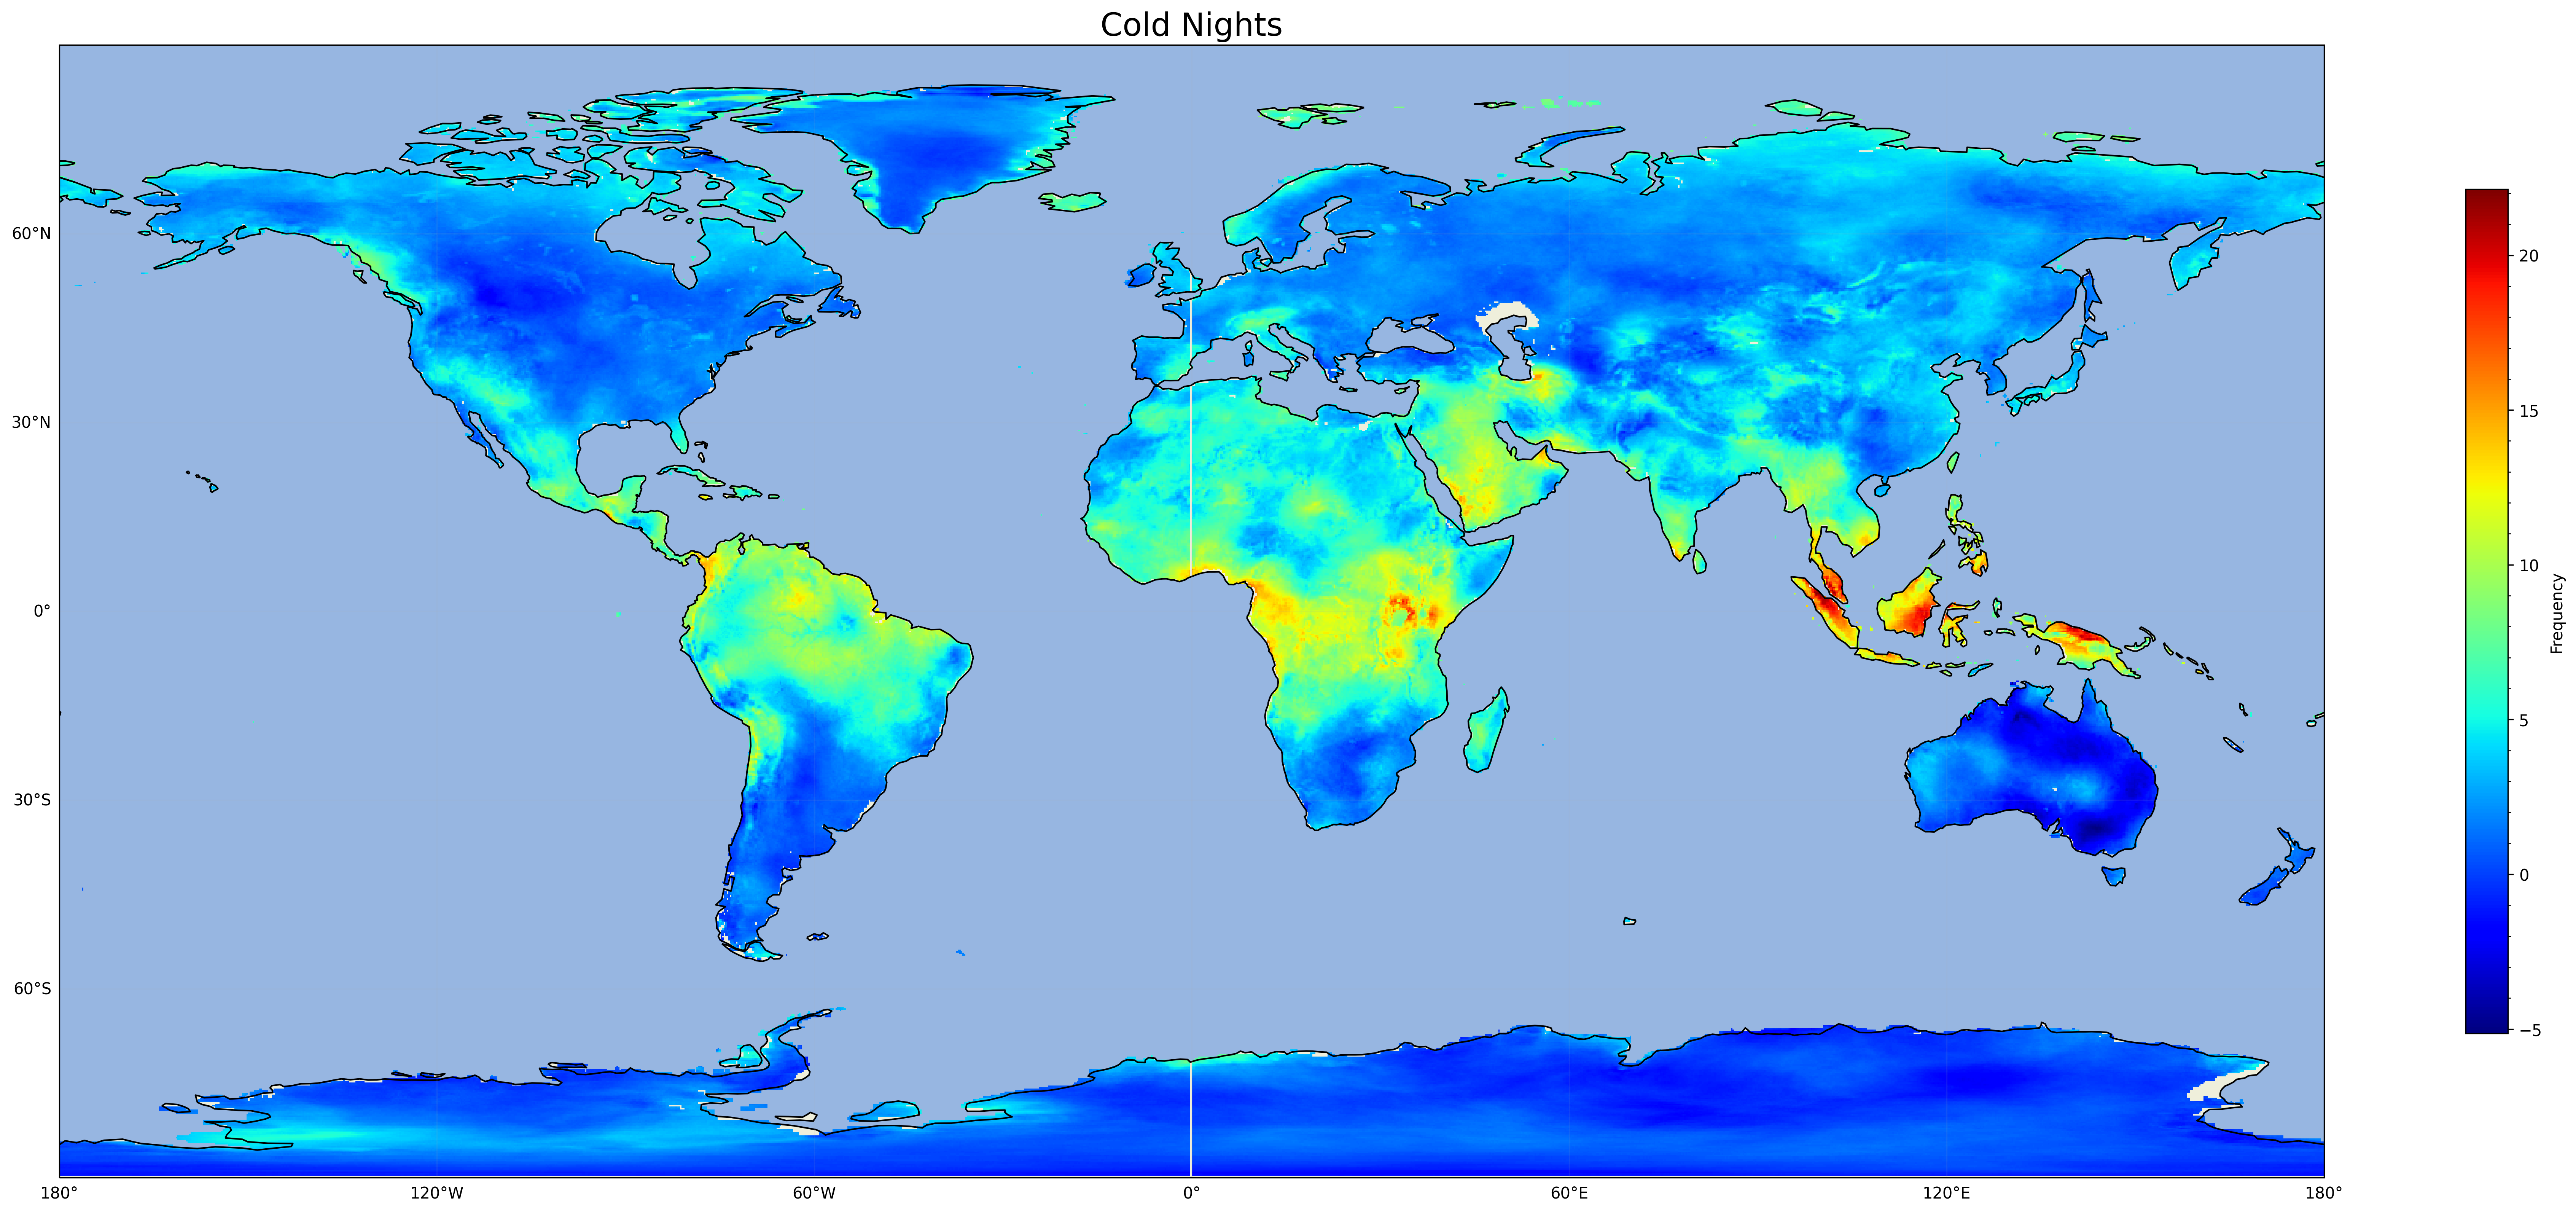
\includegraphics[width=0.80\textwidth]{/home/shiv/Documents/GitHub/EES405/clim_indices/final_plots/tn10p.png}
    \caption{Cold Nights Spatial Plot}
    \label{fig:cold_nights_spatial}
\end{figure}
From the above spatial plot of Cold Night anomalies calculated from the \textbf{TN10p} climate index, we can see that the frequency of cold nights have decreased globally.\\
The decrease in the frequency of cold nights globally can be attributed to the overall warming of the planet due to climate change. As the planet warms, the average temperature increases, and cold temperatures become less common.
\subsection{Temporal Plot  for 'Cold Nights (TN10p)'}

\begin{figure}[htb]
    \centering
    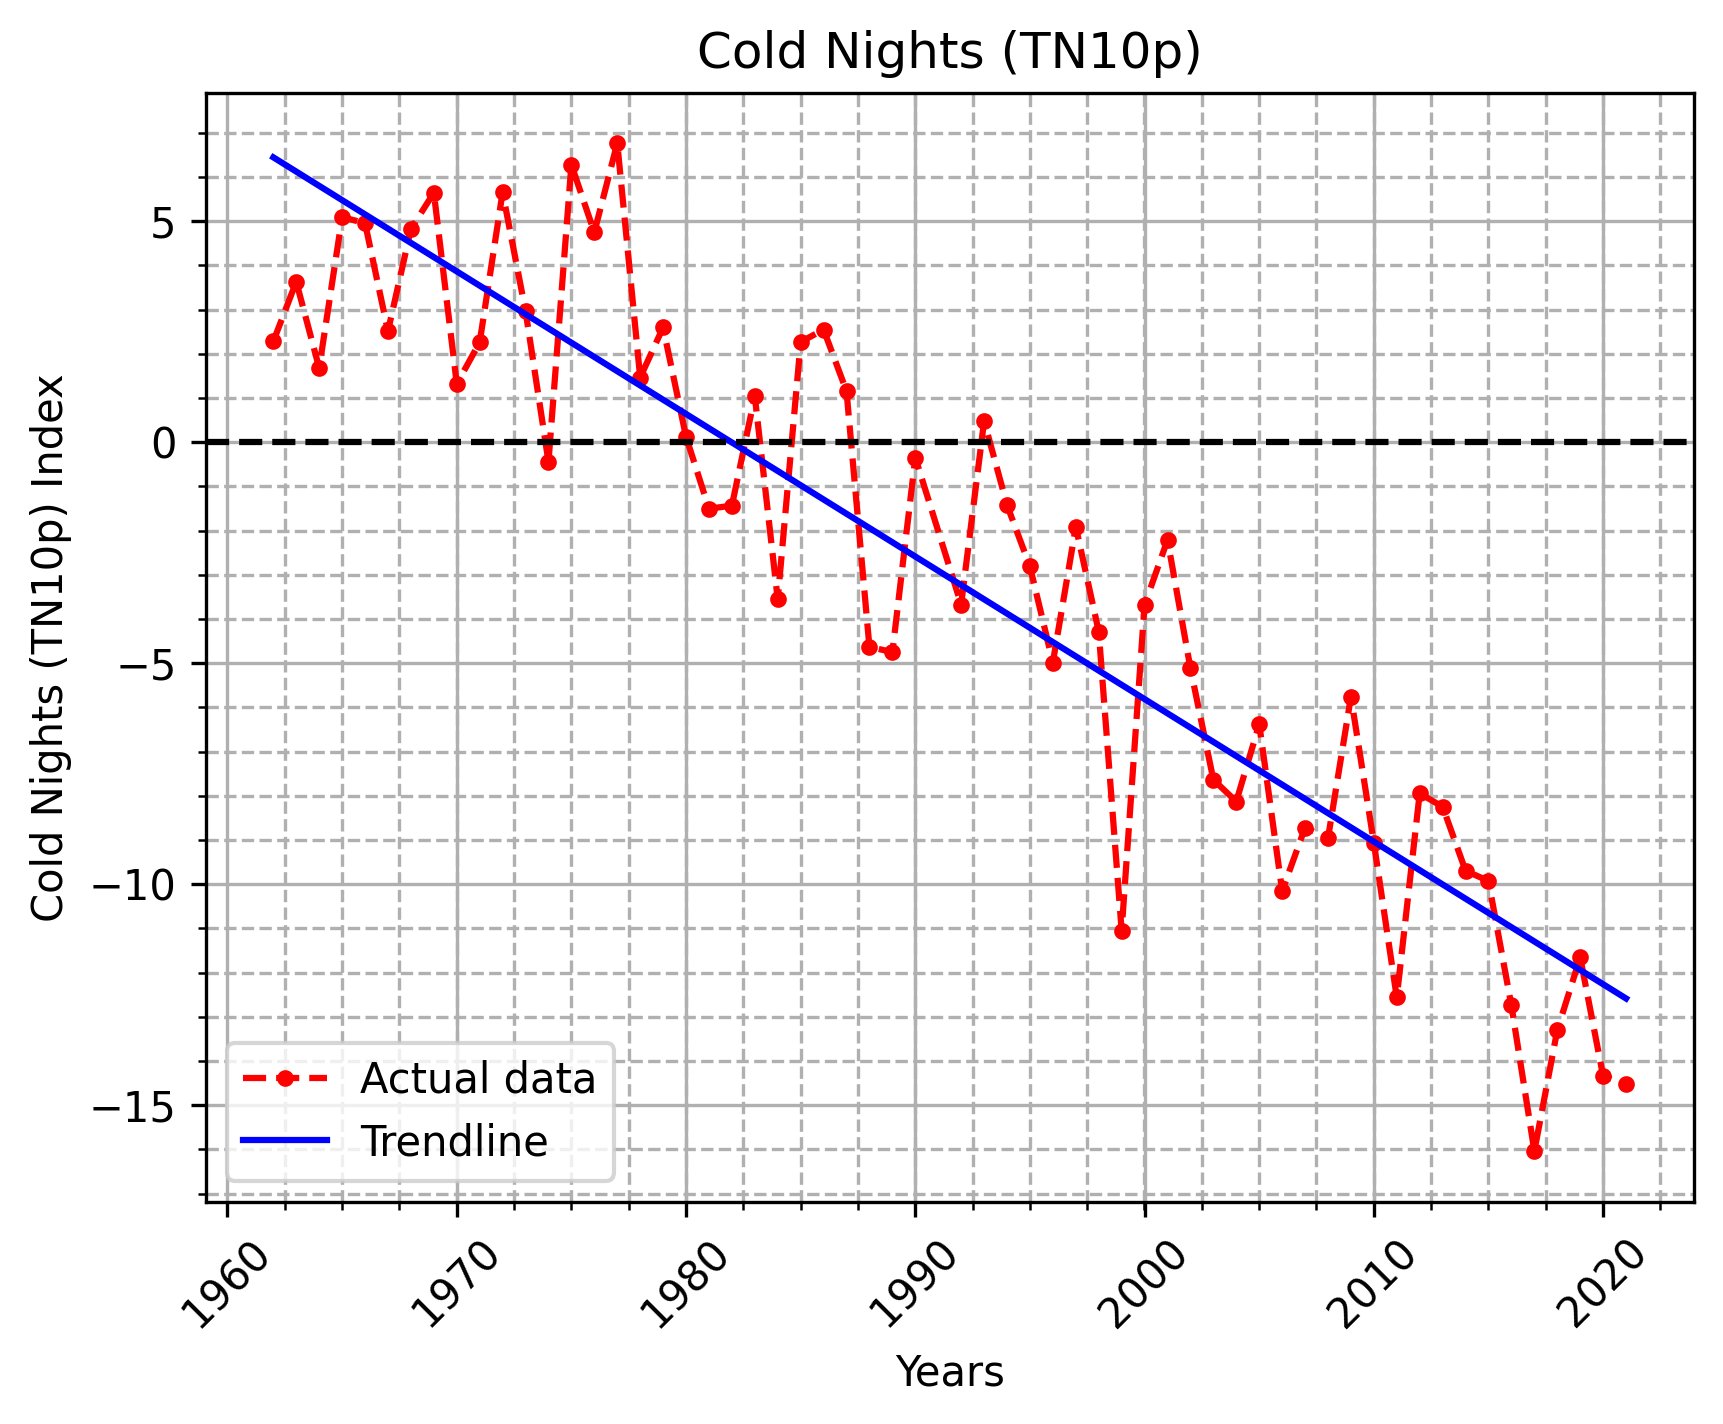
\includegraphics[width=0.80\textwidth]{/home/shiv/Documents/GitHub/EES405/clim_indices/final_plots/cold_nights_timeseries.png}
    \caption{Cold Nights temporal Plot}
    \label{fig:cold_nights_temporal}
\end{figure}

In the above time series plot of cold-nights anomalies calculated from the \textbf{TN10p} climate index, we have added a non-linear trendline with polynomial fit of degree 21 (as used in the paper by )given by the following equation. \\

$y = 2.93\times10^{0} x^{20} -2.68\times10^{-3} x^{19} +1.87\times10^{-6} x^{18} +2.20\times10^{-9} x^{17} -1.11\times10^{-12} x^{16} -4.43\times10^{-16} x^{15} +2.92\times10^{-19} x^{14} -1.05\times10^{-24} x^{13} -2.91\times10^{-26} x^{12} +6.97\times10^{-30} x^{11} +2.79\times10^{-35} x^{10} -3.35\times10^{-37} x^{9} +8.48\times10^{-41} x^{8} -1.20\times10^{-44} x^{7} +1.14\times10^{-48} x^{6} -7.67\times10^{-53} x^{5} +3.67\times10^{-57} x^{4} -1.24\times10^{-61} x^{3} +2.79\times10^{-66} x^{2} -3.78\times10^{-71} x^{1} +2.34\times10^{-76}$

The decrease in the frequency of cold nights is consistent with the overall warming of the planet due to climate change as seen in the above spatial plot.\\
Overall, the decrease in the frequency of cold nights is a consistent and expected result of the overall warming of the planet due to climate change.

\section{Warm Nights}
Plot the spatial and temporal plot of the warm nights anomalies for the time-period 1960-2020 using 1960-1990 as the reference time period from era5 dataset.\\

\subsection{Spatial plot for 'Warm Nights (TN90p)'}
\begin{figure}[htb]
    \centering
    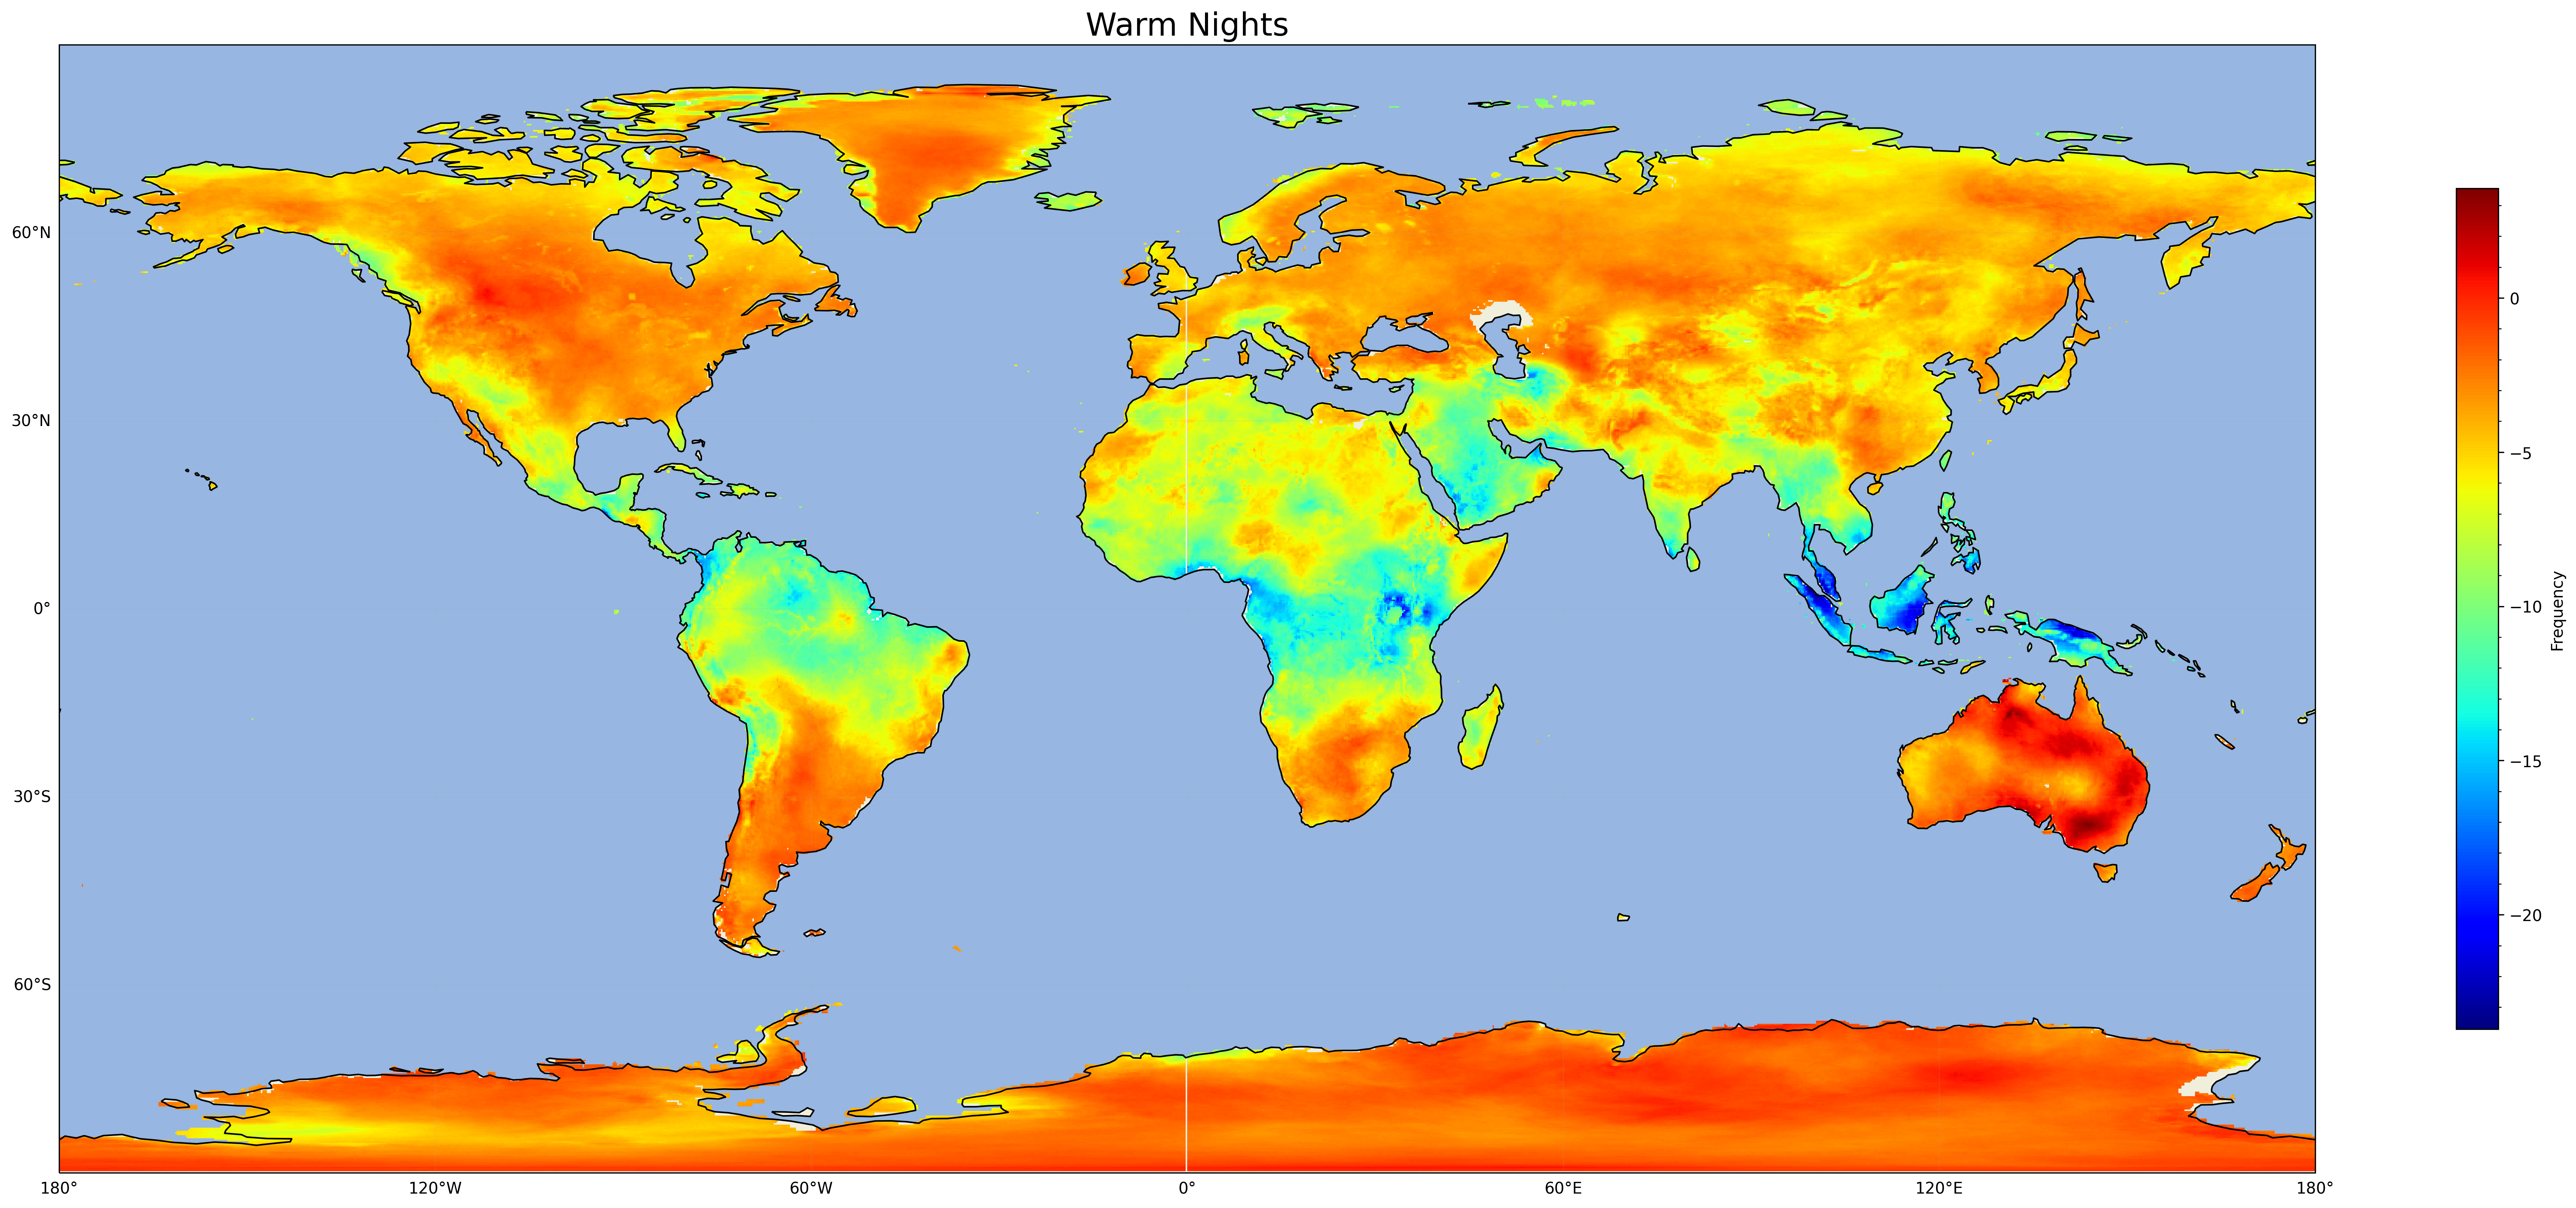
\includegraphics[width=0.80\textwidth]{/home/shiv/Documents/GitHub/EES405/clim_indices/final_plots/tn90p.png}
    \caption{Warm Nights Spatial Plot}
    \label{fig:warm_nights_spatial}
\end{figure}
From the above spatial plot of Cold Night anomalies calculated from the \textbf{TN10p} climate index, we can see that the frequency of cold nights have decreased globally.\\
The decrease in the frequency of cold nights globally can be attributed to the overall warming of the planet due to climate change. As the planet warms, the average temperature increases, and cold temperatures become less common.
\subsection{Temporal Plot  for 'Warm Nights (TN90p)'}

\begin{figure}[htb]
    \centering
    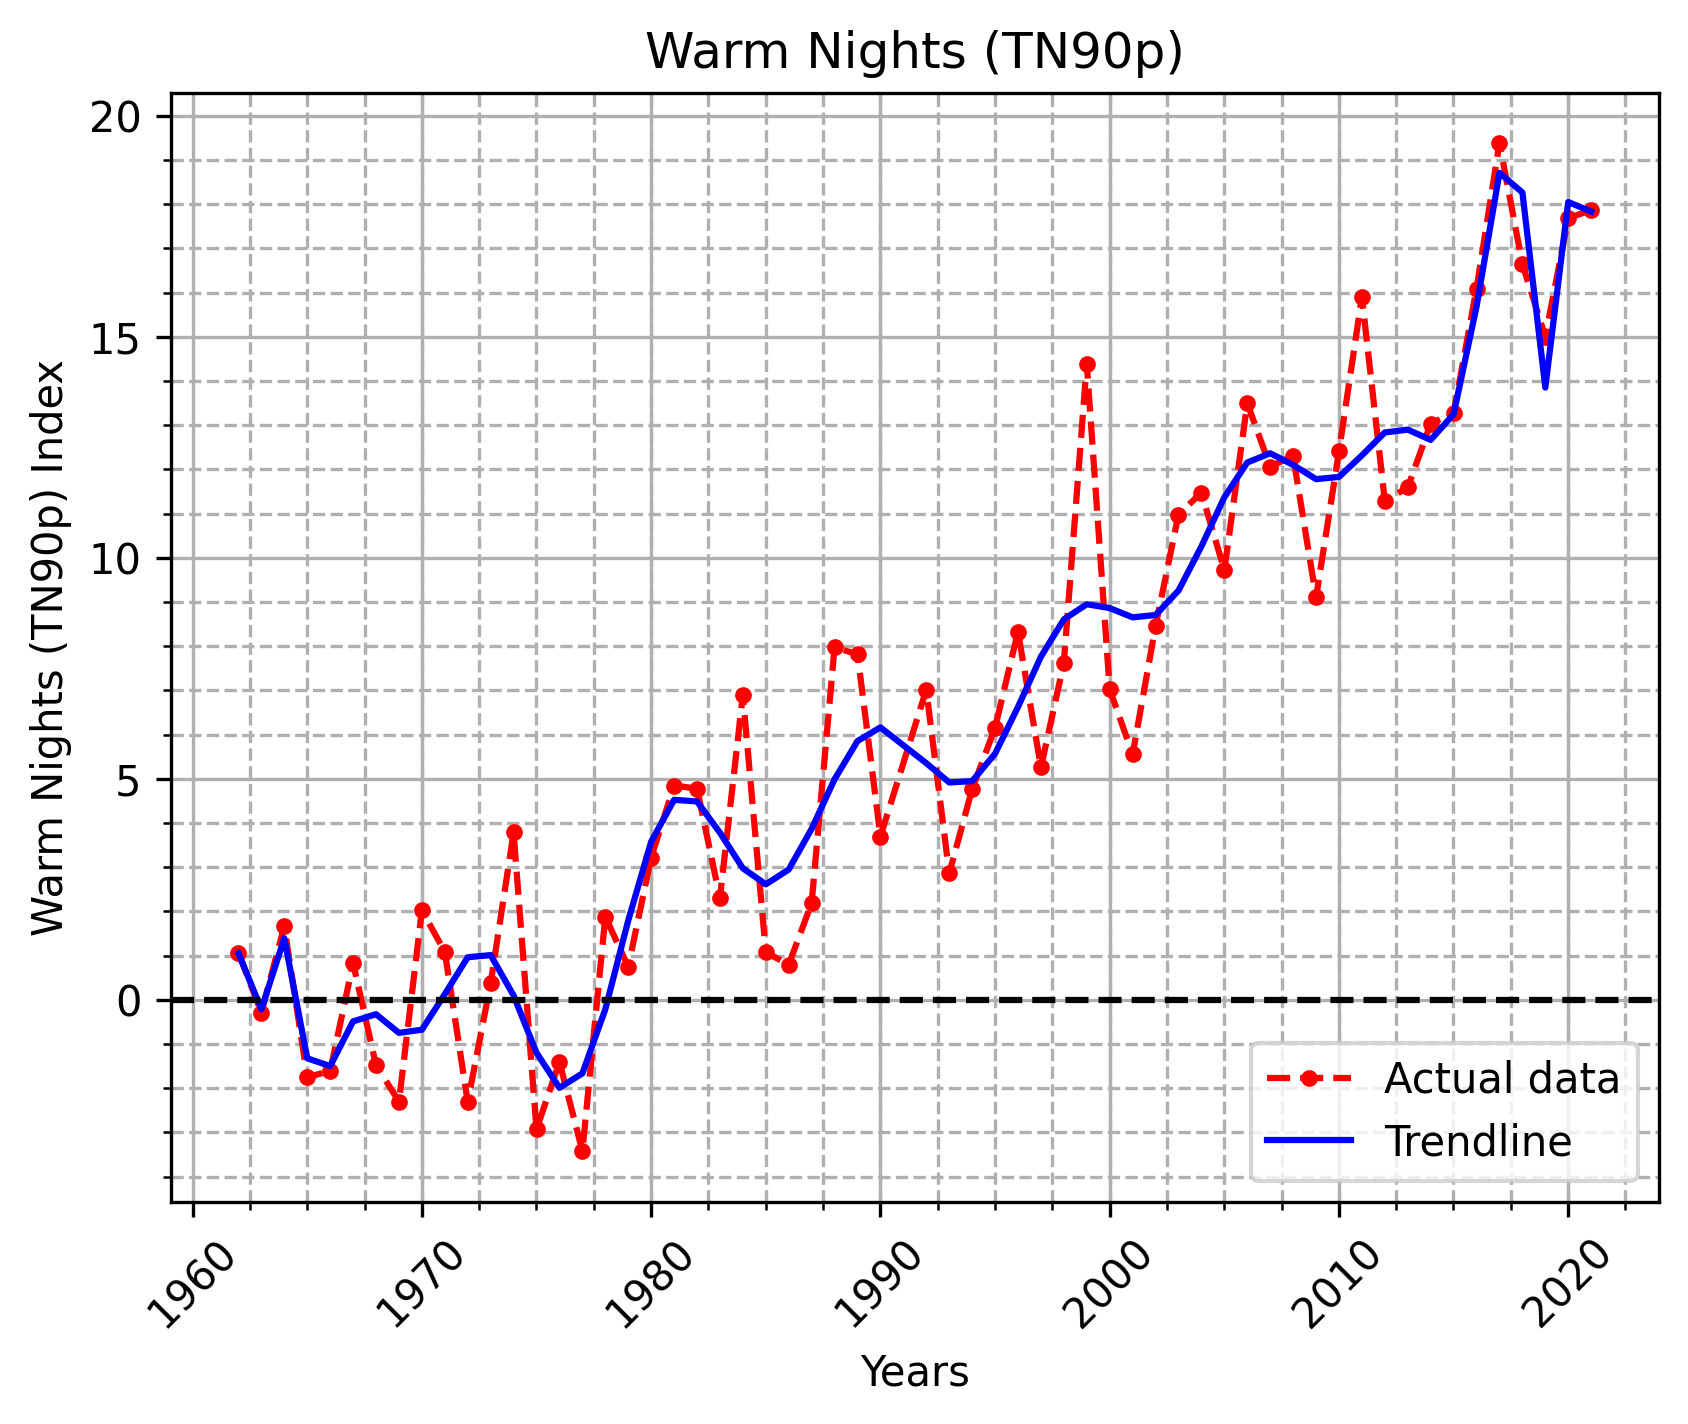
\includegraphics[width=0.80\textwidth]{/home/shiv/Documents/GitHub/EES405/clim_indices/final_plots/warm_nights_timeseries.png}
    \caption{Warm Nights temporal Plot}
    \label{fig:warm_nights_temporal}
\end{figure}

In the above time series plot of cold-nights anomalies calculated from the \textbf{TN10p} climate index, we have added a non-linear trendline with polynomial fit of degree 21 (as used in the paper by )given by the following equation. \\

$y = 2.93\times10^{0} x^{20} -2.68\times10^{-3} x^{19} +1.87\times10^{-6} x^{18} +2.20\times10^{-9} x^{17} -1.11\times10^{-12} x^{16} -4.43\times10^{-16} x^{15} +2.92\times10^{-19} x^{14} -1.05\times10^{-24} x^{13} -2.91\times10^{-26} x^{12} +6.97\times10^{-30} x^{11} +2.79\times10^{-35} x^{10} -3.35\times10^{-37} x^{9} +8.48\times10^{-41} x^{8} -1.20\times10^{-44} x^{7} +1.14\times10^{-48} x^{6} -7.67\times10^{-53} x^{5} +3.67\times10^{-57} x^{4} -1.24\times10^{-61} x^{3} +2.79\times10^{-66} x^{2} -3.78\times10^{-71} x^{1} +2.34\times10^{-76}$

The decrease in the frequency of cold nights is consistent with the overall warming of the planet due to climate change as seen in the above spatial plot.\\
Overall, the decrease in the frequency of cold nights is a consistent and expected result of the overall warming of the planet due to climate change.

\section{Cold Days}


\subsection{Spatial plot for 'Cold Days (TX10p)'}
\begin{figure}[htb]
    \centering
    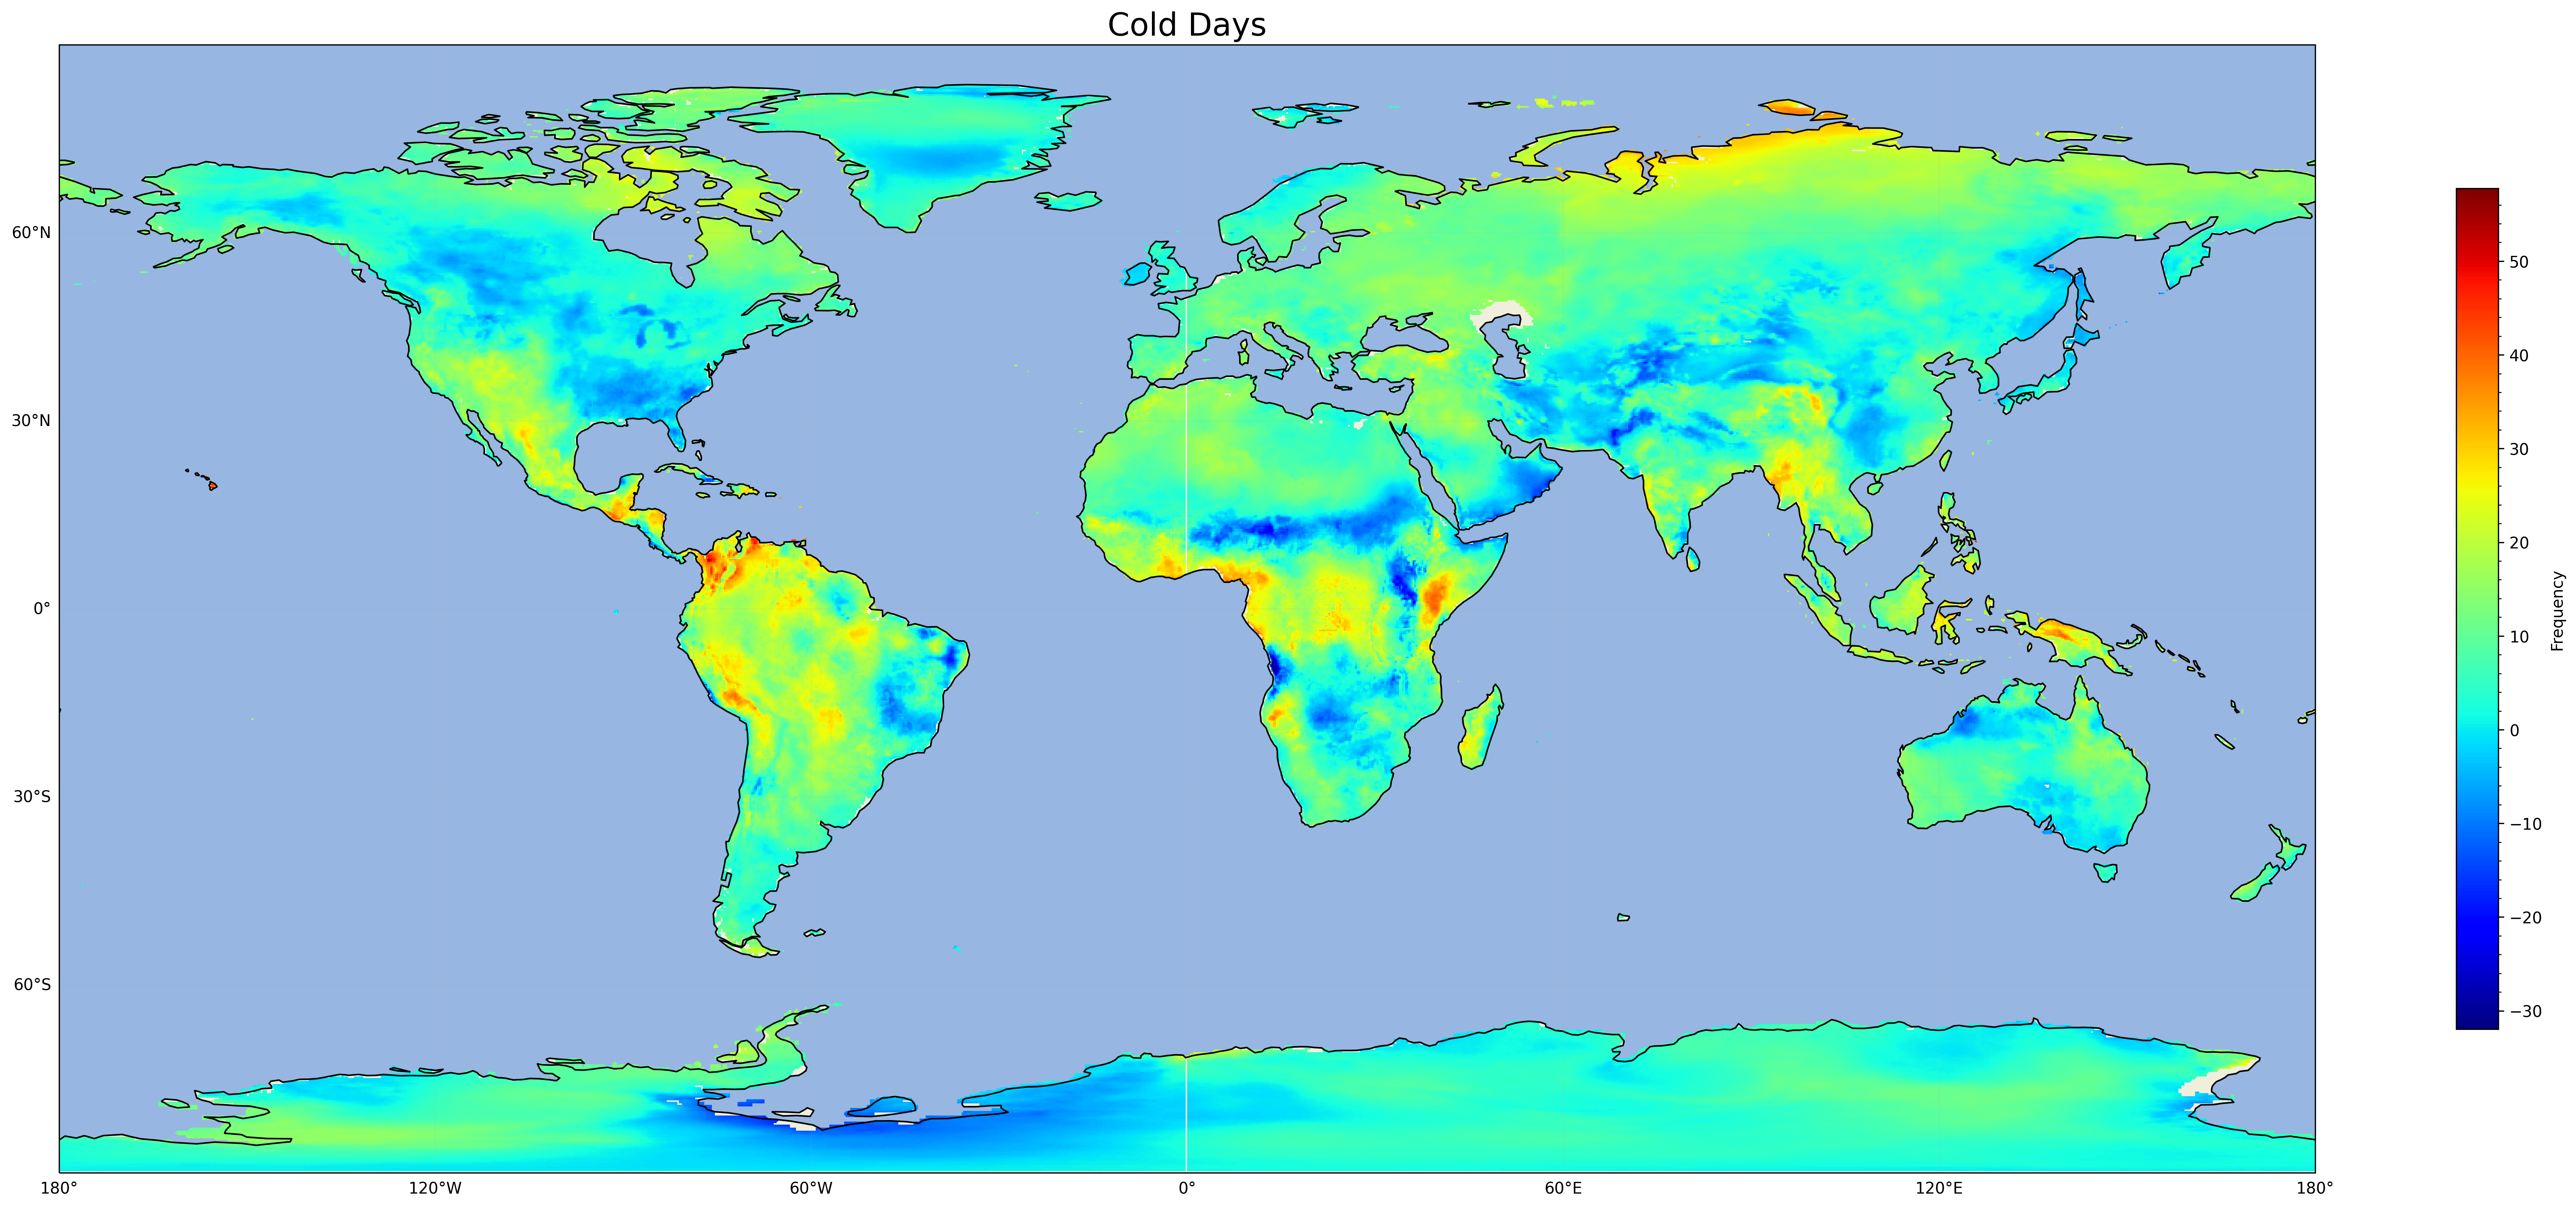
\includegraphics[width=0.80\textwidth]{/home/shiv/Documents/GitHub/EES405/clim_indices/final_plots/tx10p.png}
    \caption{Cold Days Spatial Plot}
    \label{fig:cold_days_spatial}
\end{figure}

\subsection{Temporal Plot for 'Cold Days (TX10p)'}
In the above time series plot of cold-days anomalies calculated from the \textbf{TX10p} climate index, we have added a non-linear trendline with polynomial fit of degree 21 (as used in the paper by )given by the following equation. \\

$ y = 2.70 \times 10^{0}x^{21} - 1.45 \times 10^{-3}x^{20} - 1.21 \times 10^{-6}x^{19} + 1.33 \times 10^{-9}x^{18} + 1.44 \times 10^{-12}x^{17} - 7.46 \times 10^{-16}x^{16} - 3.40 \times 10^{-19}x^{15} + 2.25 \times 10^{-22}x^{14} - 5.15 \times 10^{-28}x^{13} - 2.44 \times 10^{-29}x^{12} + 6.13 \times 10^{-33}x^{11} - 7.94 \times 10^{-39}x^{10} - 3.03 \times 10^{-40}x^{9} + 7.96 \times 10^{-44}x^{8} - 1.16 \times 10^{-47}x^{7} + 1.12 \times 10^{-51}x^{6} - 7.65 \times 10^{-56}x^{5} + 3.69 \times 10^{-60}x^{4} - 1.24 \times 10^{-64}x^{3} + 2.79 \times 10^{-69}x^{2} - 3.75 \times 10^{-74}x^{1} + 2.29 \times 10^{-79}
$

\begin{figure}[htb]
    \centering
    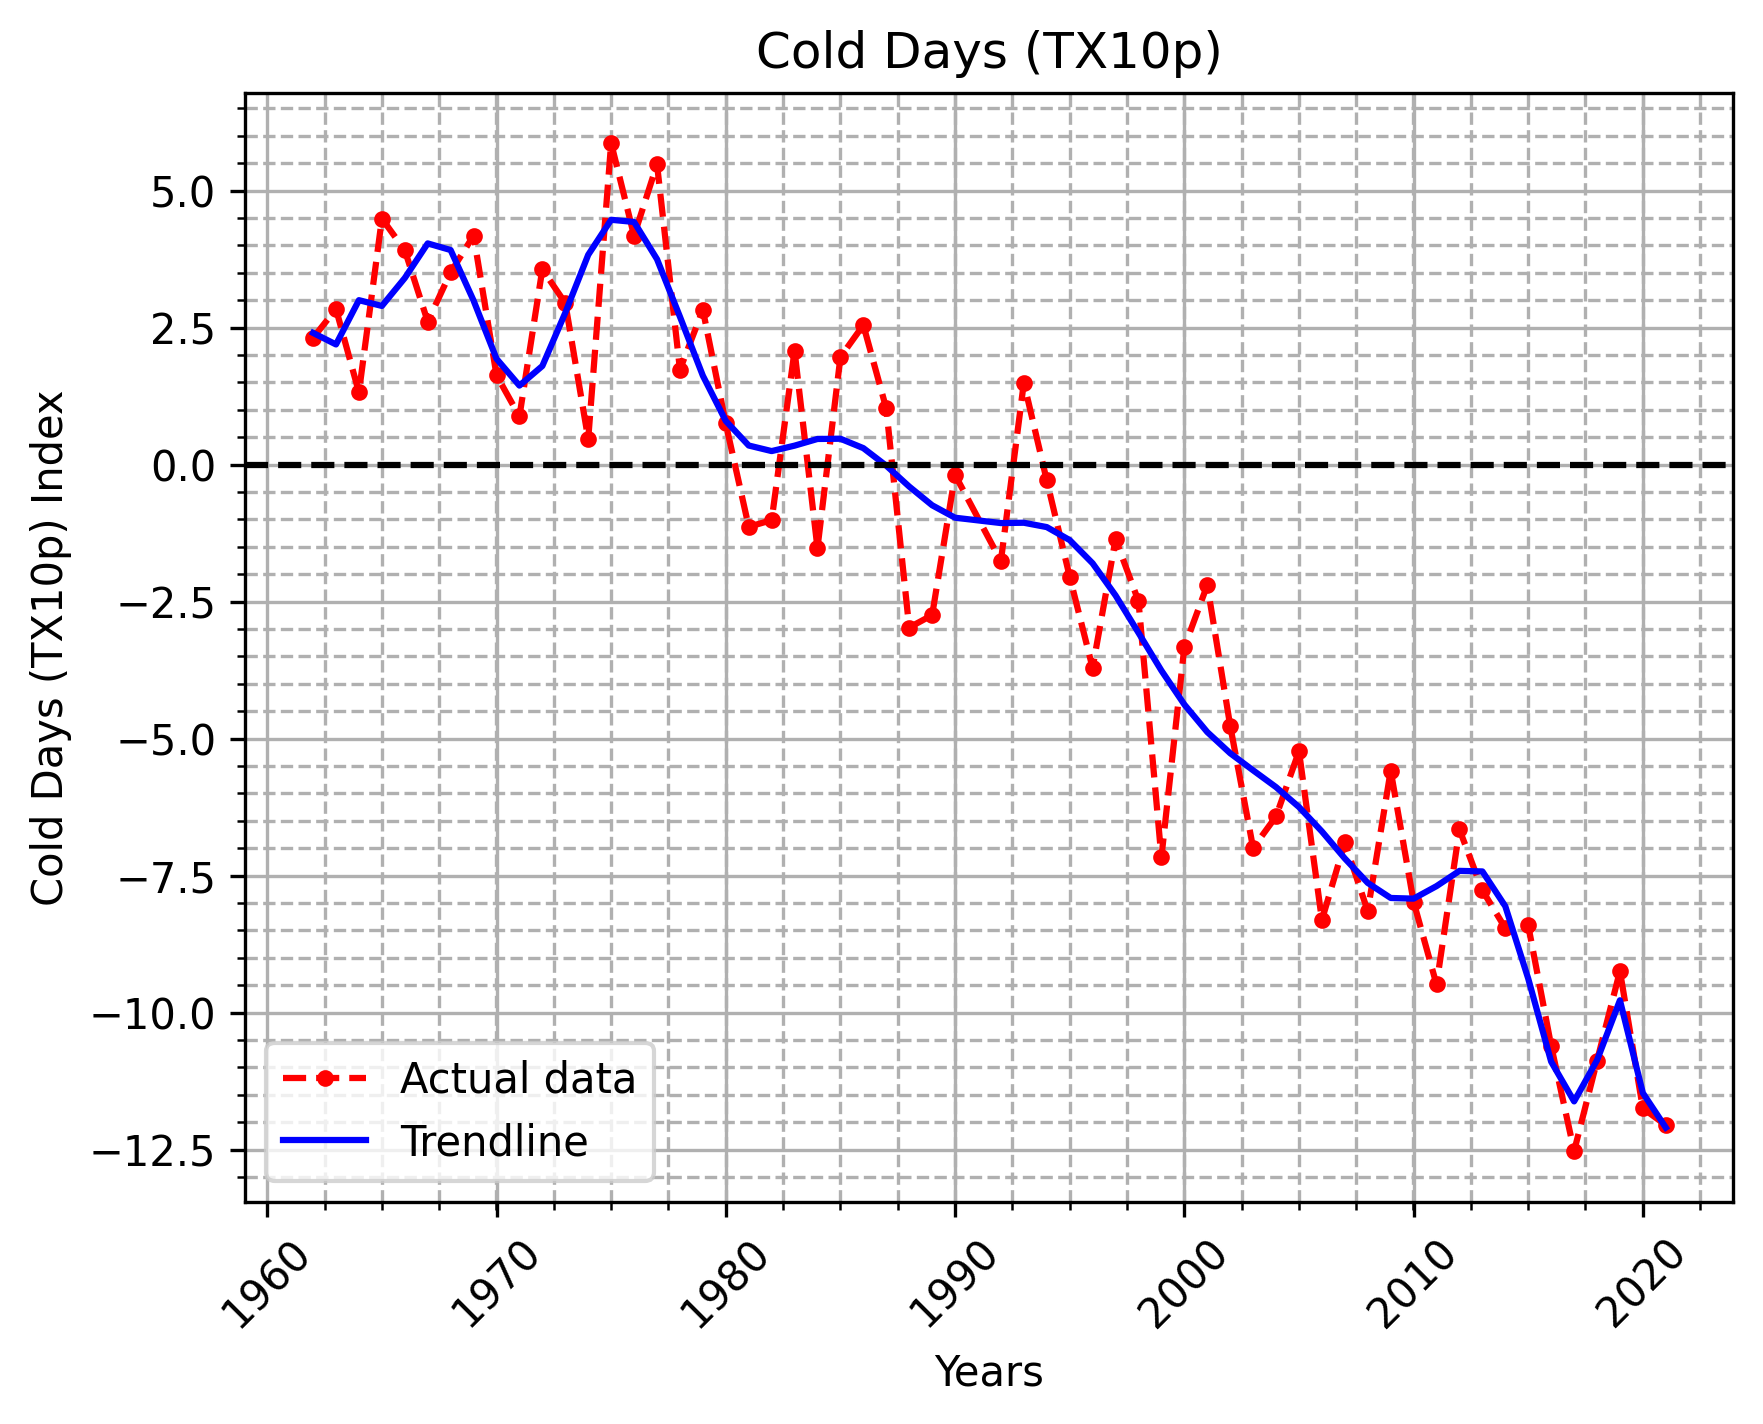
\includegraphics[width=0.80\textwidth]{//home/shiv/Documents/GitHub/EES405/clim_indices/final_plots/cold_days_timeseries.png}
    \caption{Cold days temporal Plot}
    \label{fig:cold_days_temporal}
\end{figure}

The decrease in the frequency of cold days is consistent with the overall warming of the planet due to climate change as seen in the above spatial plot.\\
Overall, the decrease in the frequency of cold nights is a consistent and expected result of the overall warming of the planet due to climate change.

\section{Warm Days}
\newpage
\subsection{Spatial plot for 'Warm Days (TX90p)'}

\begin{figure}[htb]
    \centering
    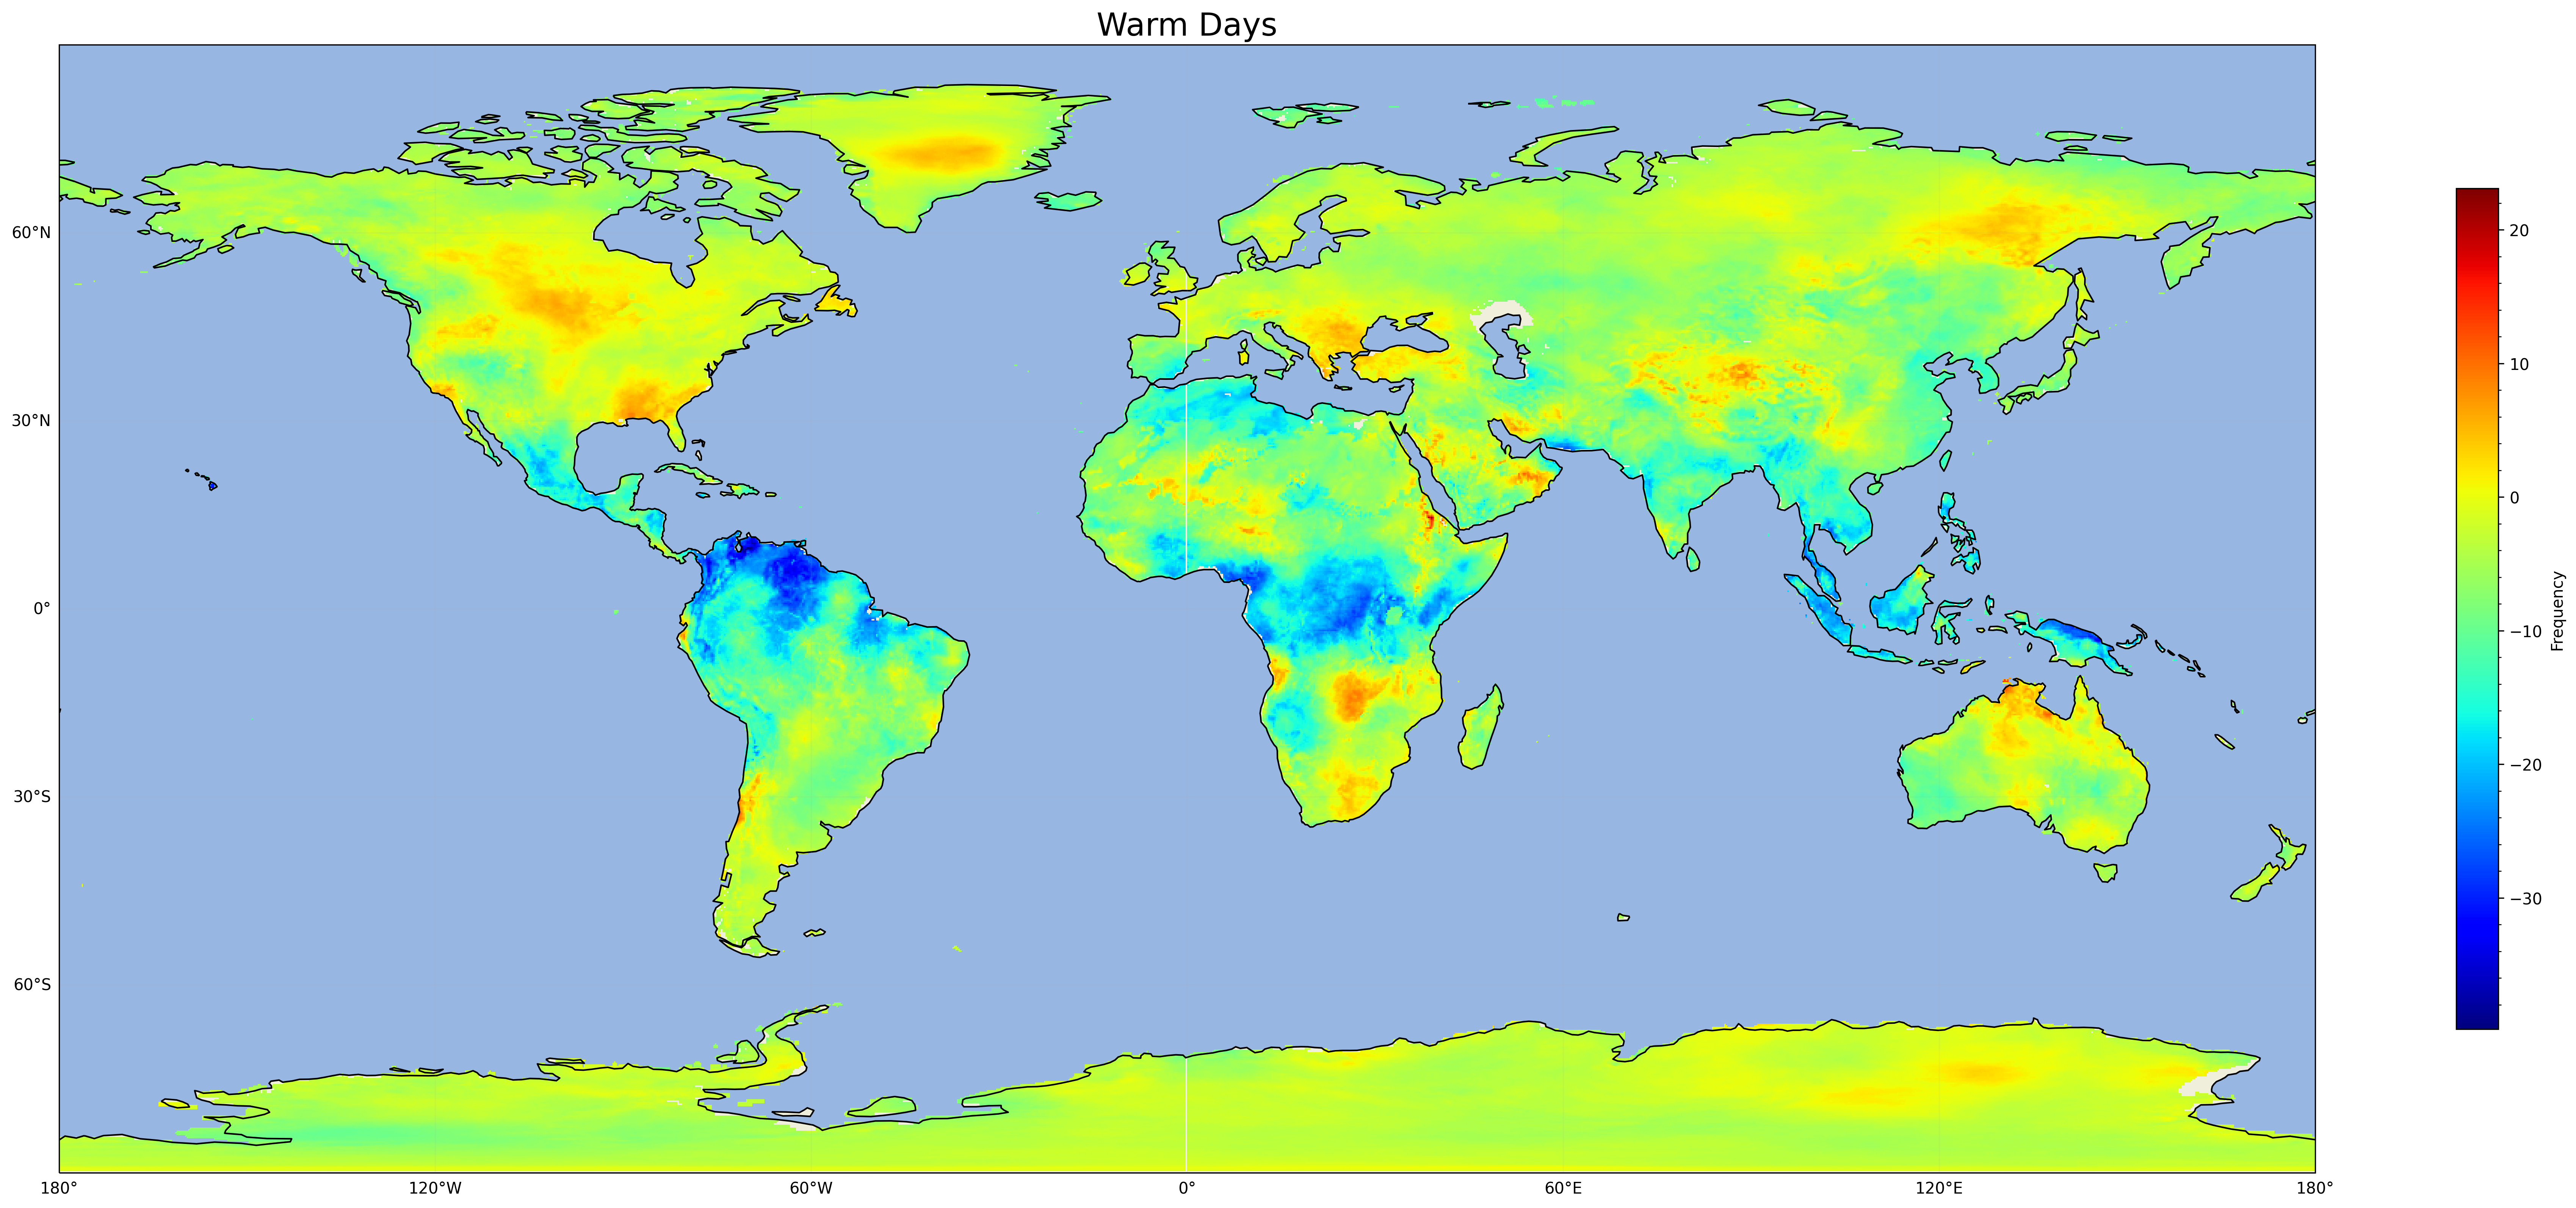
\includegraphics[width=0.80\textwidth]{/home/shiv/Documents/GitHub/EES405/clim_indices/final_plots/tx90p.png}
    \caption{Warm days Spatial Plot}
    \label{fig:warm_days_spatial}
\end{figure}

\subsection{Temporal Plot for 'Warm Days (TX90p)'}
In the above time series plot of warm-days anomalies calculated from the \textbf{TX90p} climate index, we have added a non-linear trendline with polynomial fit of degree 21 (as used in the paper by )given by the following equation. \\
\begin{figure}[htb]
    \centering
    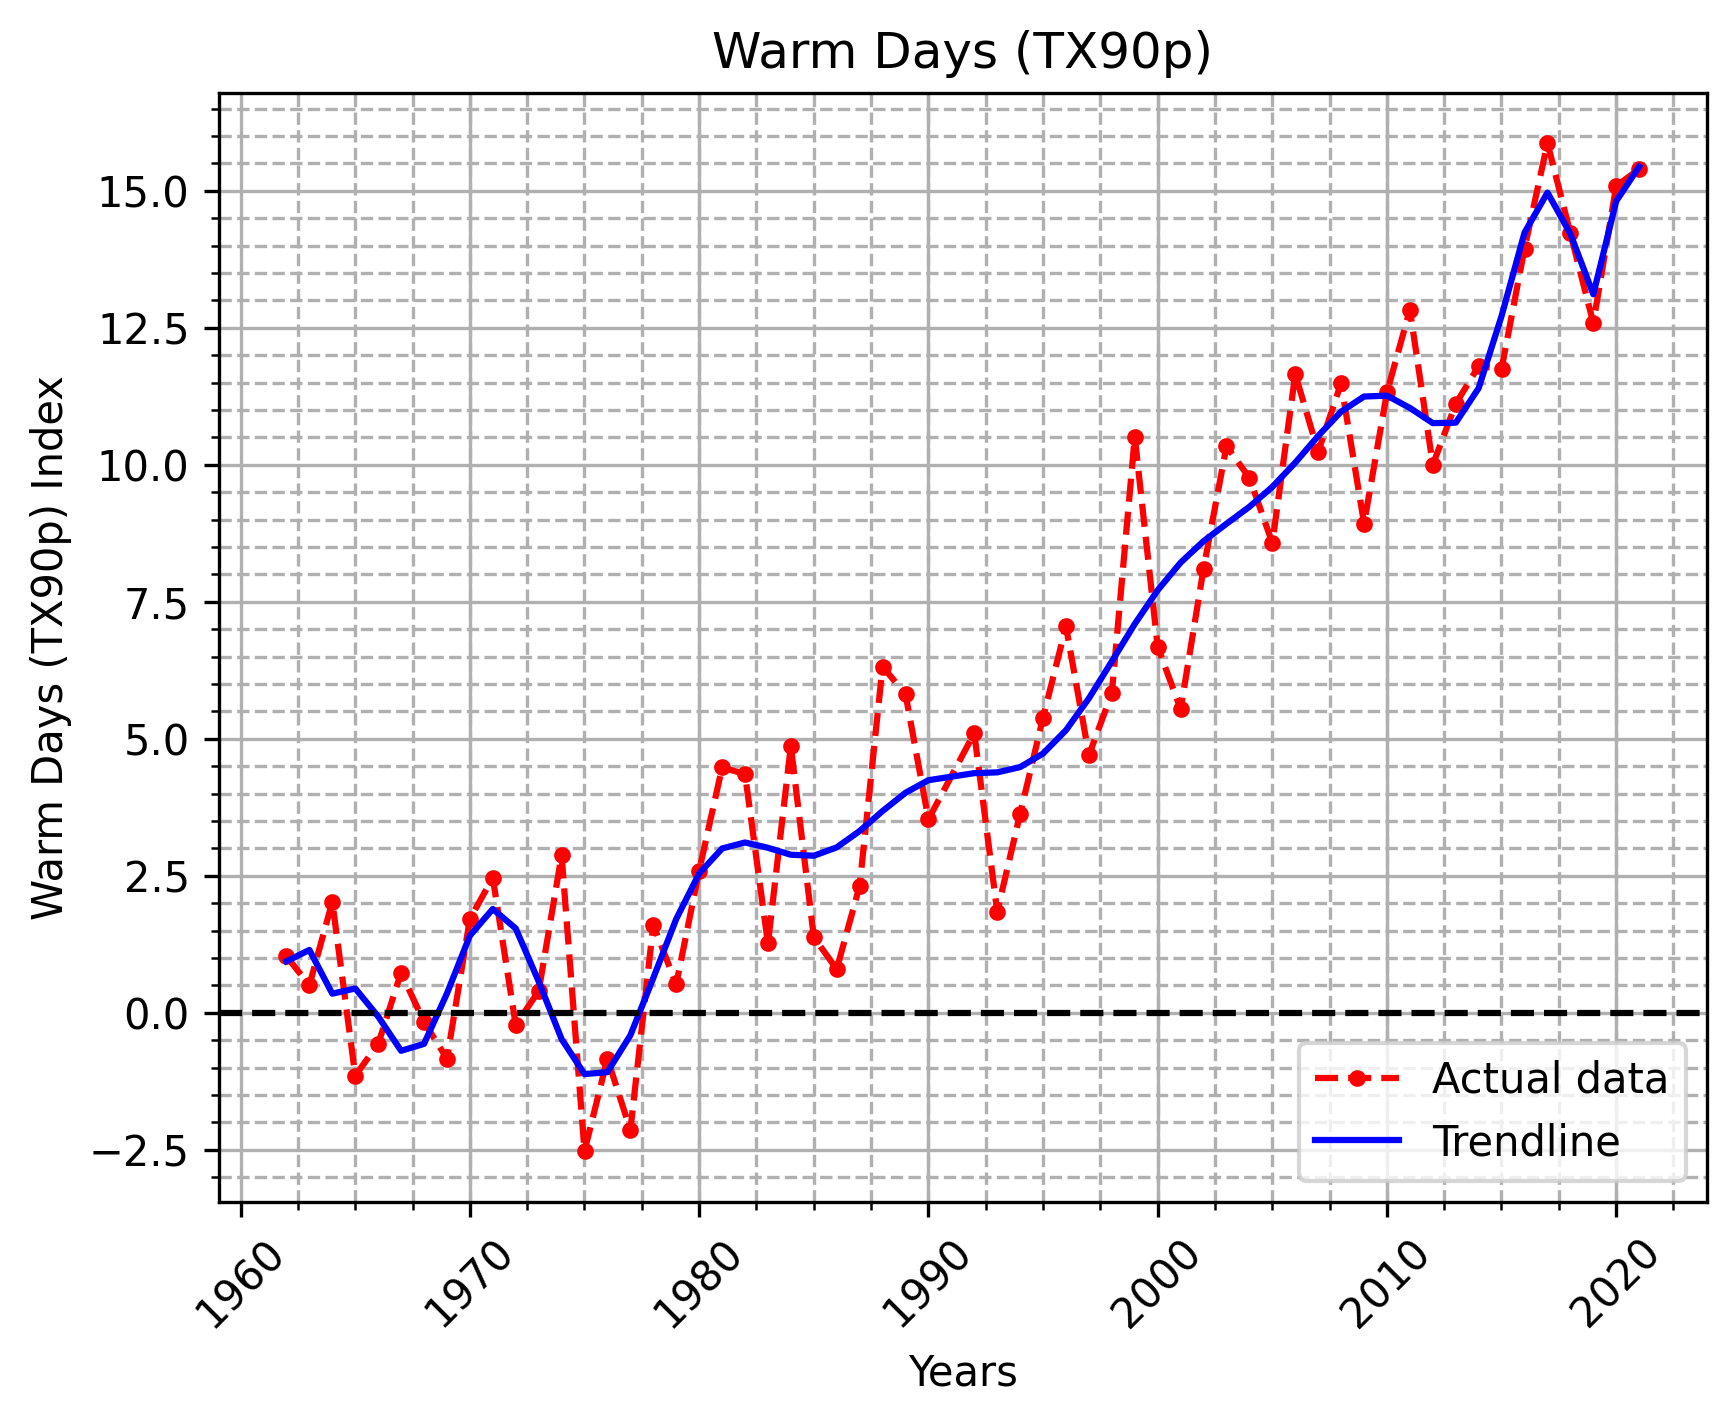
\includegraphics[width=0.75\textwidth]{//home/shiv/Documents/GitHub/EES405/clim_indices/final_plots/warm_days_timeseries.png}
    \caption{Warm days temporal Plot}
    \label{fig:warm_days_temporal}
\end{figure}

$ y = 6.45 \times 10^{-1}x^{21} + 1.44 \times 10^{-3}x^{20} + 1.18 \times 10^{-6}x^{19} - 1.32 \times 10^{-9}x^{18} - 1.42 \times 10^{-12}x^{17} + 7.38 \times 10^{-16}x^{16} + 3.37 \times 10^{-19}x^{15} - 2.23 \times 10^{-22}x^{14} + 4.12 \times 10^{-28}x^{13} + 2.42 \times 10^{-29}x^{12} - 6.06 \times 10^{-33}x^{11} + 6.37 \times 10^{-39}x^{10} + 3.00 \times 10^{-40}x^{9} - 7.88 \times 10^{-44}x^{8} + 1.15 \times 10^{-47}x^{7} - 1.11 \times 10^{-51}x^{6} + 7.58 \times 10^{-56}x^{5} - 3.66 \times 10^{-60}x^{4} + 1.23 \times 10^{-64}x^{3} - 2.76 \times 10^{-69}x^{2} + 3.72 \times 10^{-74}x^{1} - 2.27 \times 10^{-79}$

The increase in the frequency of warm days is consistent with the overall warming of the planet due to climate change as seen in the above spatial plot.\\
Overall, the increase in the frequency of warm days is a consistent and expected result of the overall warming of the planet due to climate change.

\section{Cold Spells}
\subsection{Spatial plot for 'Cold spells (CWFI)'}

\begin{figure}[htb]
    \centering
    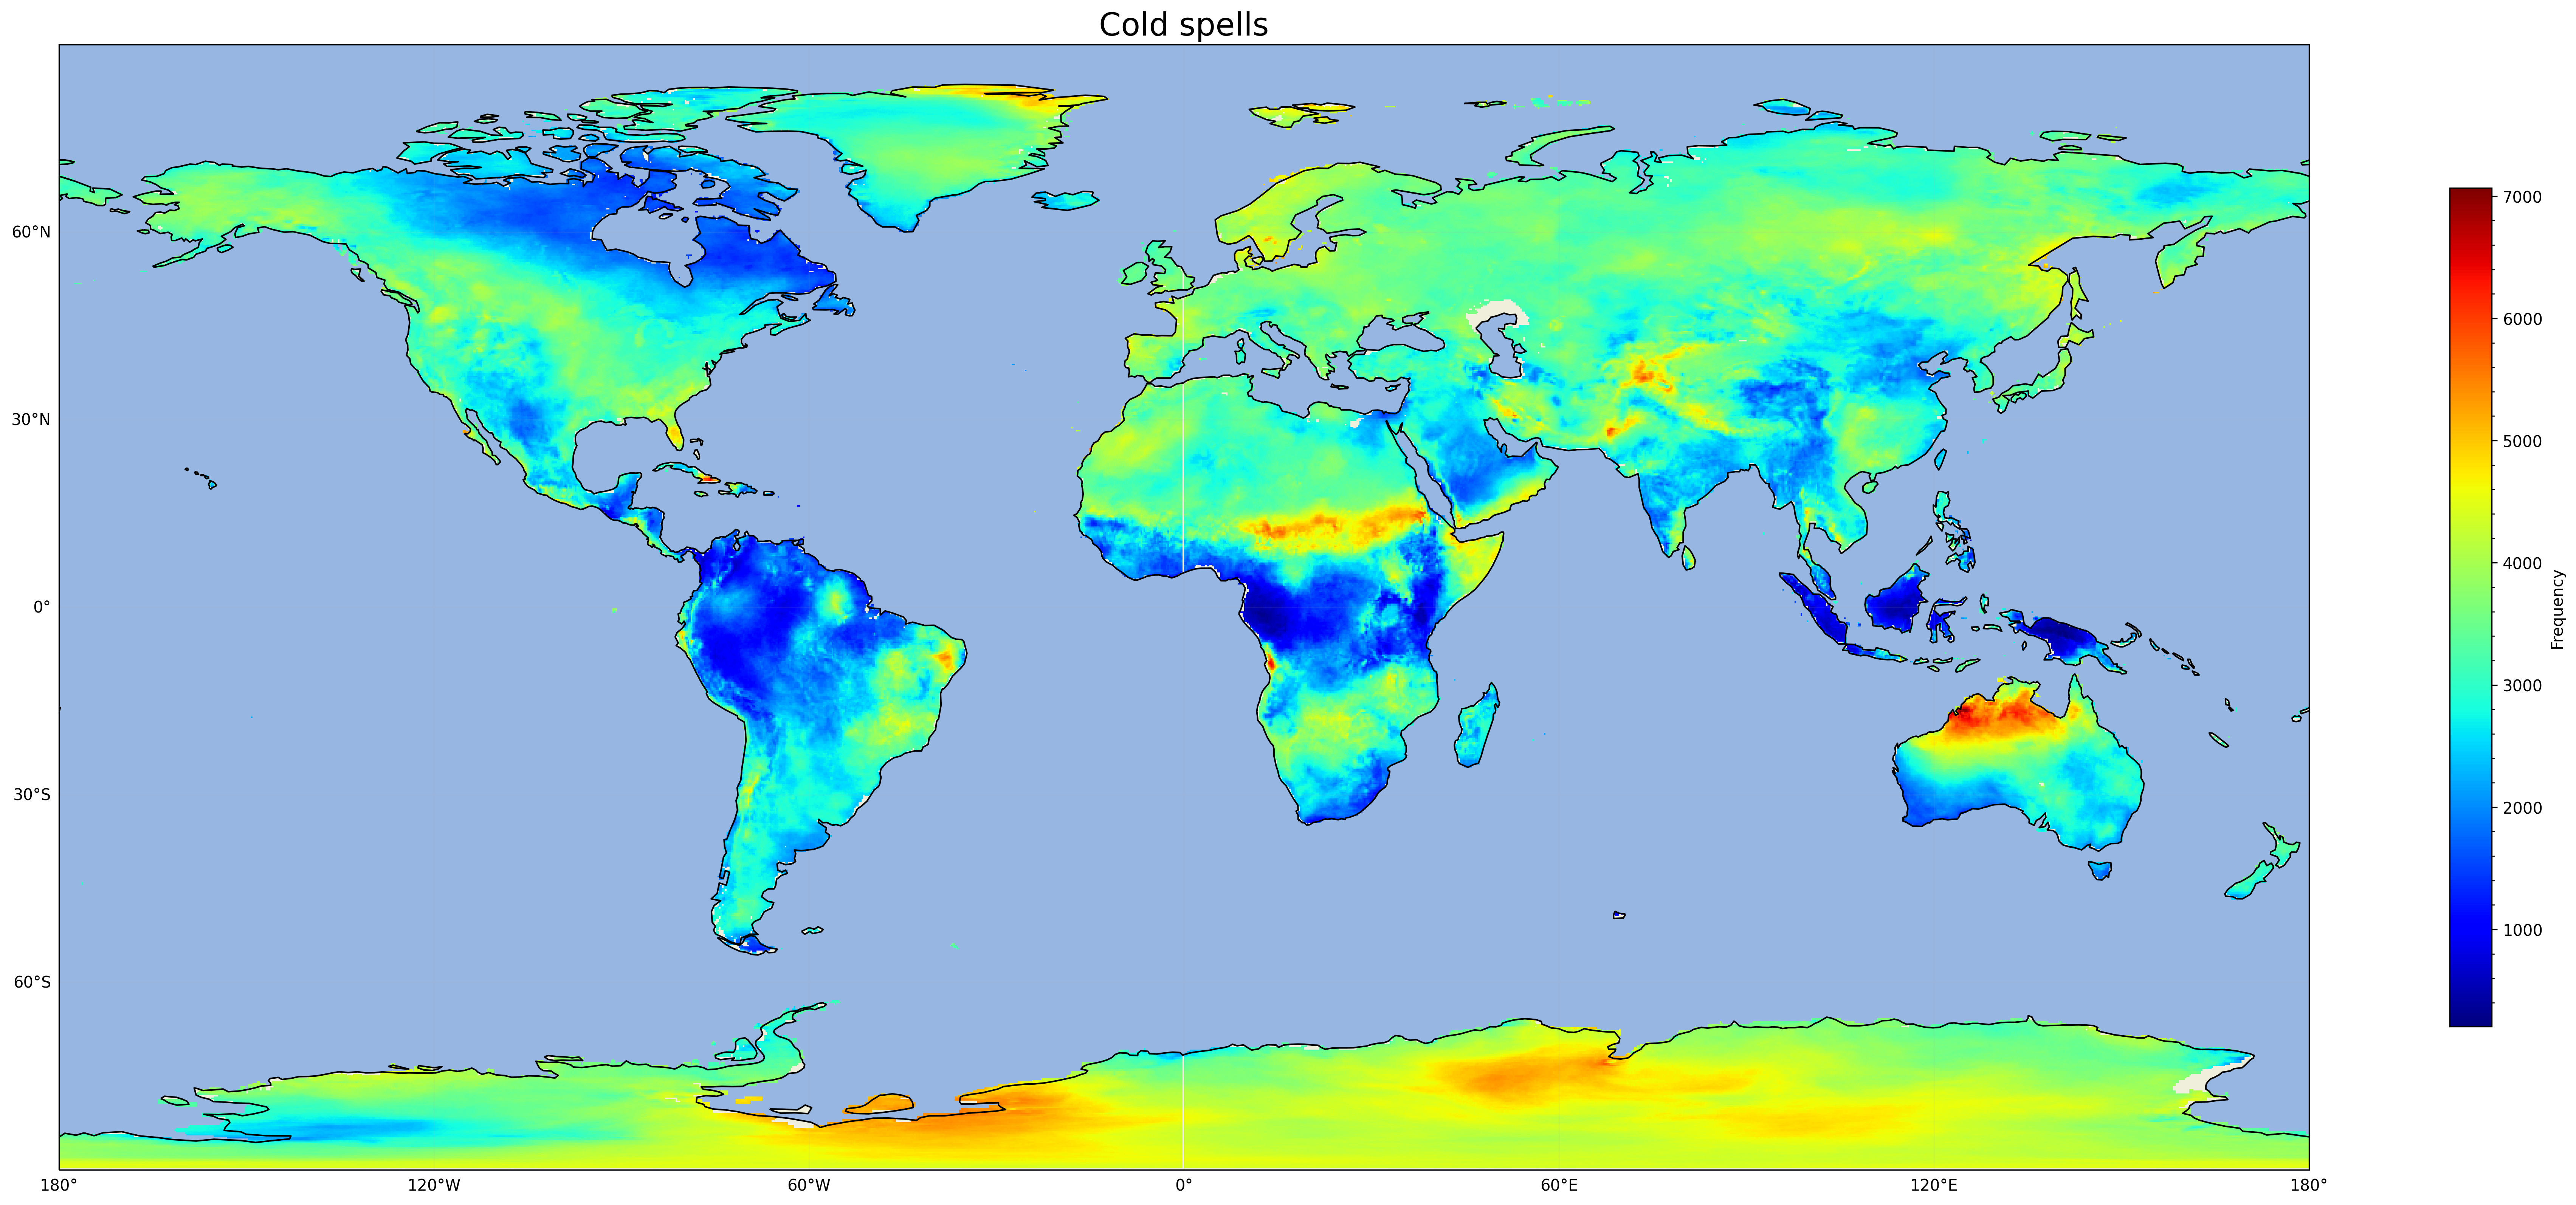
\includegraphics[width=0.80\textwidth]{/home/shiv/Documents/GitHub/EES405/clim_indices/final_plots/coldpells-spatial.png}
    \caption{coldspells Spatial Plot}
    \label{fig:coldwave_spatial}
\end{figure}

\subsection{Temporal Plot for 'Cold Spells (CWFI)'}
In the above time series plot of cold spells anomalies calculated from the \textbf{CWFI} climate index, we have added a non-linear trendline with polynomial fit of degree 21 (as used in the paper by )given by the following equation. \\
\begin{figure}[htb]
    \centering
    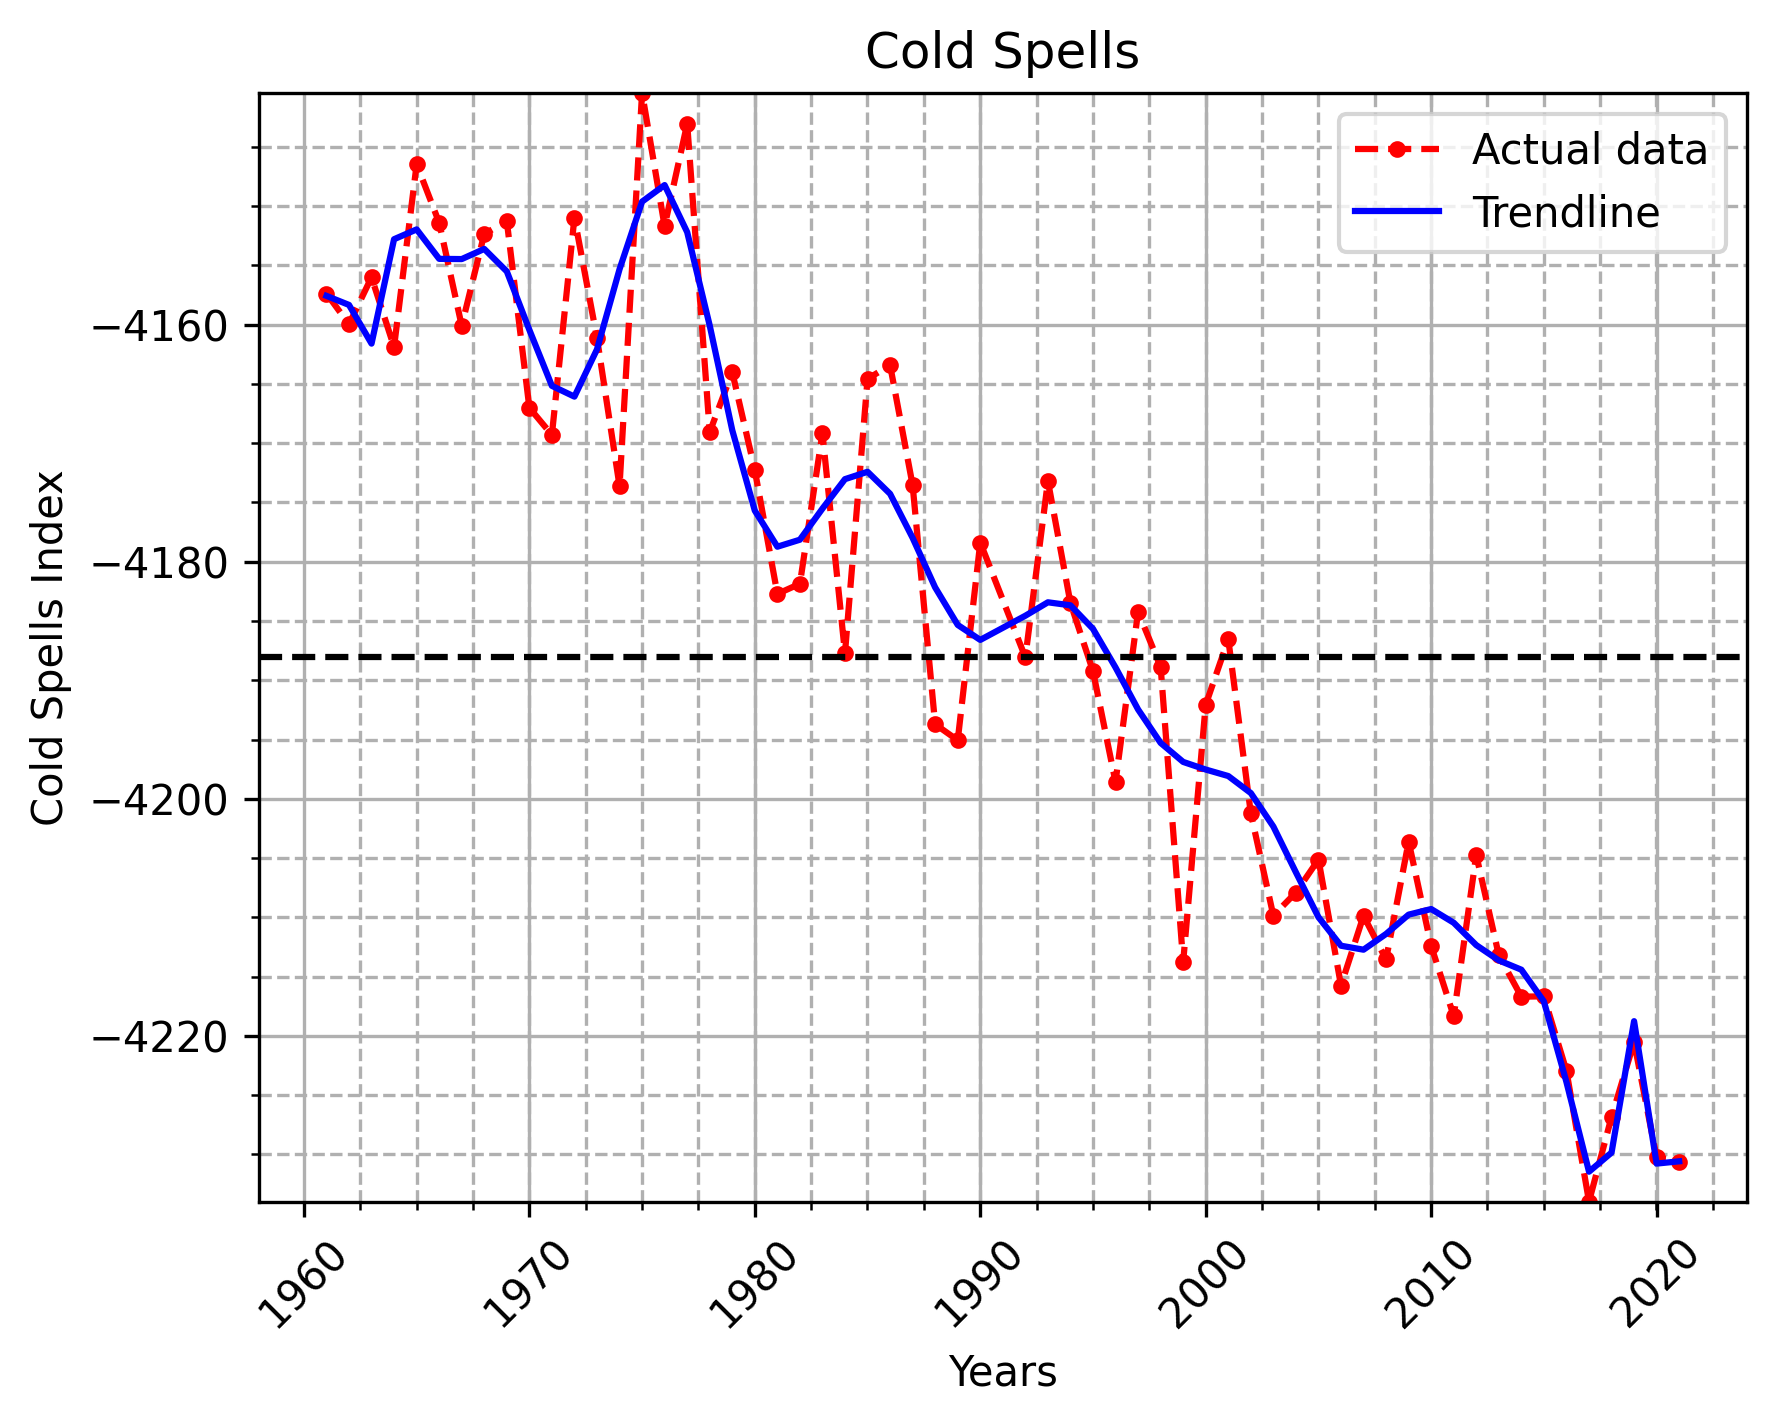
\includegraphics[width=0.75\textwidth]{//home/shiv/Documents/GitHub/EES405/clim_indices/final_plots/coldspells.png}
    \caption{Cold spells temporal Plot}
    \label{fig:coldspells_temporal}
\end{figure}

$ y = -4.16\times10^{3}x^{21}-1.51\times10^{-2}x^{20}+7.03\times10^{-7}x^{19}+1.49\times10^{-8}x^{18}+6.24\times10^{-13}x^{17}-5.27\times10^{-15}x^{16}+4.61\times10^{-19}x^{15}+7.93\times10^{-22}x^{14}-1.99\times10^{-25}x^{13}-3.21\times10^{-29}x^{12}+2.05\times10^{-32}x^{11}-2.66\times10^{-36}x^{10}-2.89\times10^{-40}x^{9}+1.54\times10^{-43}x^{8}-2.71\times10^{-47}x^{7}+2.89\times10^{-51}x^{6}-2.09\times10^{-55}x^{5}+1.05\times10^{-59}x^{4}-3.65\times10^{-64}x^{3}+8.39\times10^{-69}x^{2}-1.15\times10^{-73}x+7.12\times10^{-79}$

The decrease in the frequency of coldspells is consistent with the overall warming of the planet due to climate change as seen in the above spatial plot.\\
Overall, the decrease in the frequency of coldspells is a consistent and expected result of the overall warming of the planet due to climate change.

\section{Warm Spells}
\subsection{Spatial plot for 'Warm spells (HWFI)'}
\begin{figure}[htb]
    \centering
    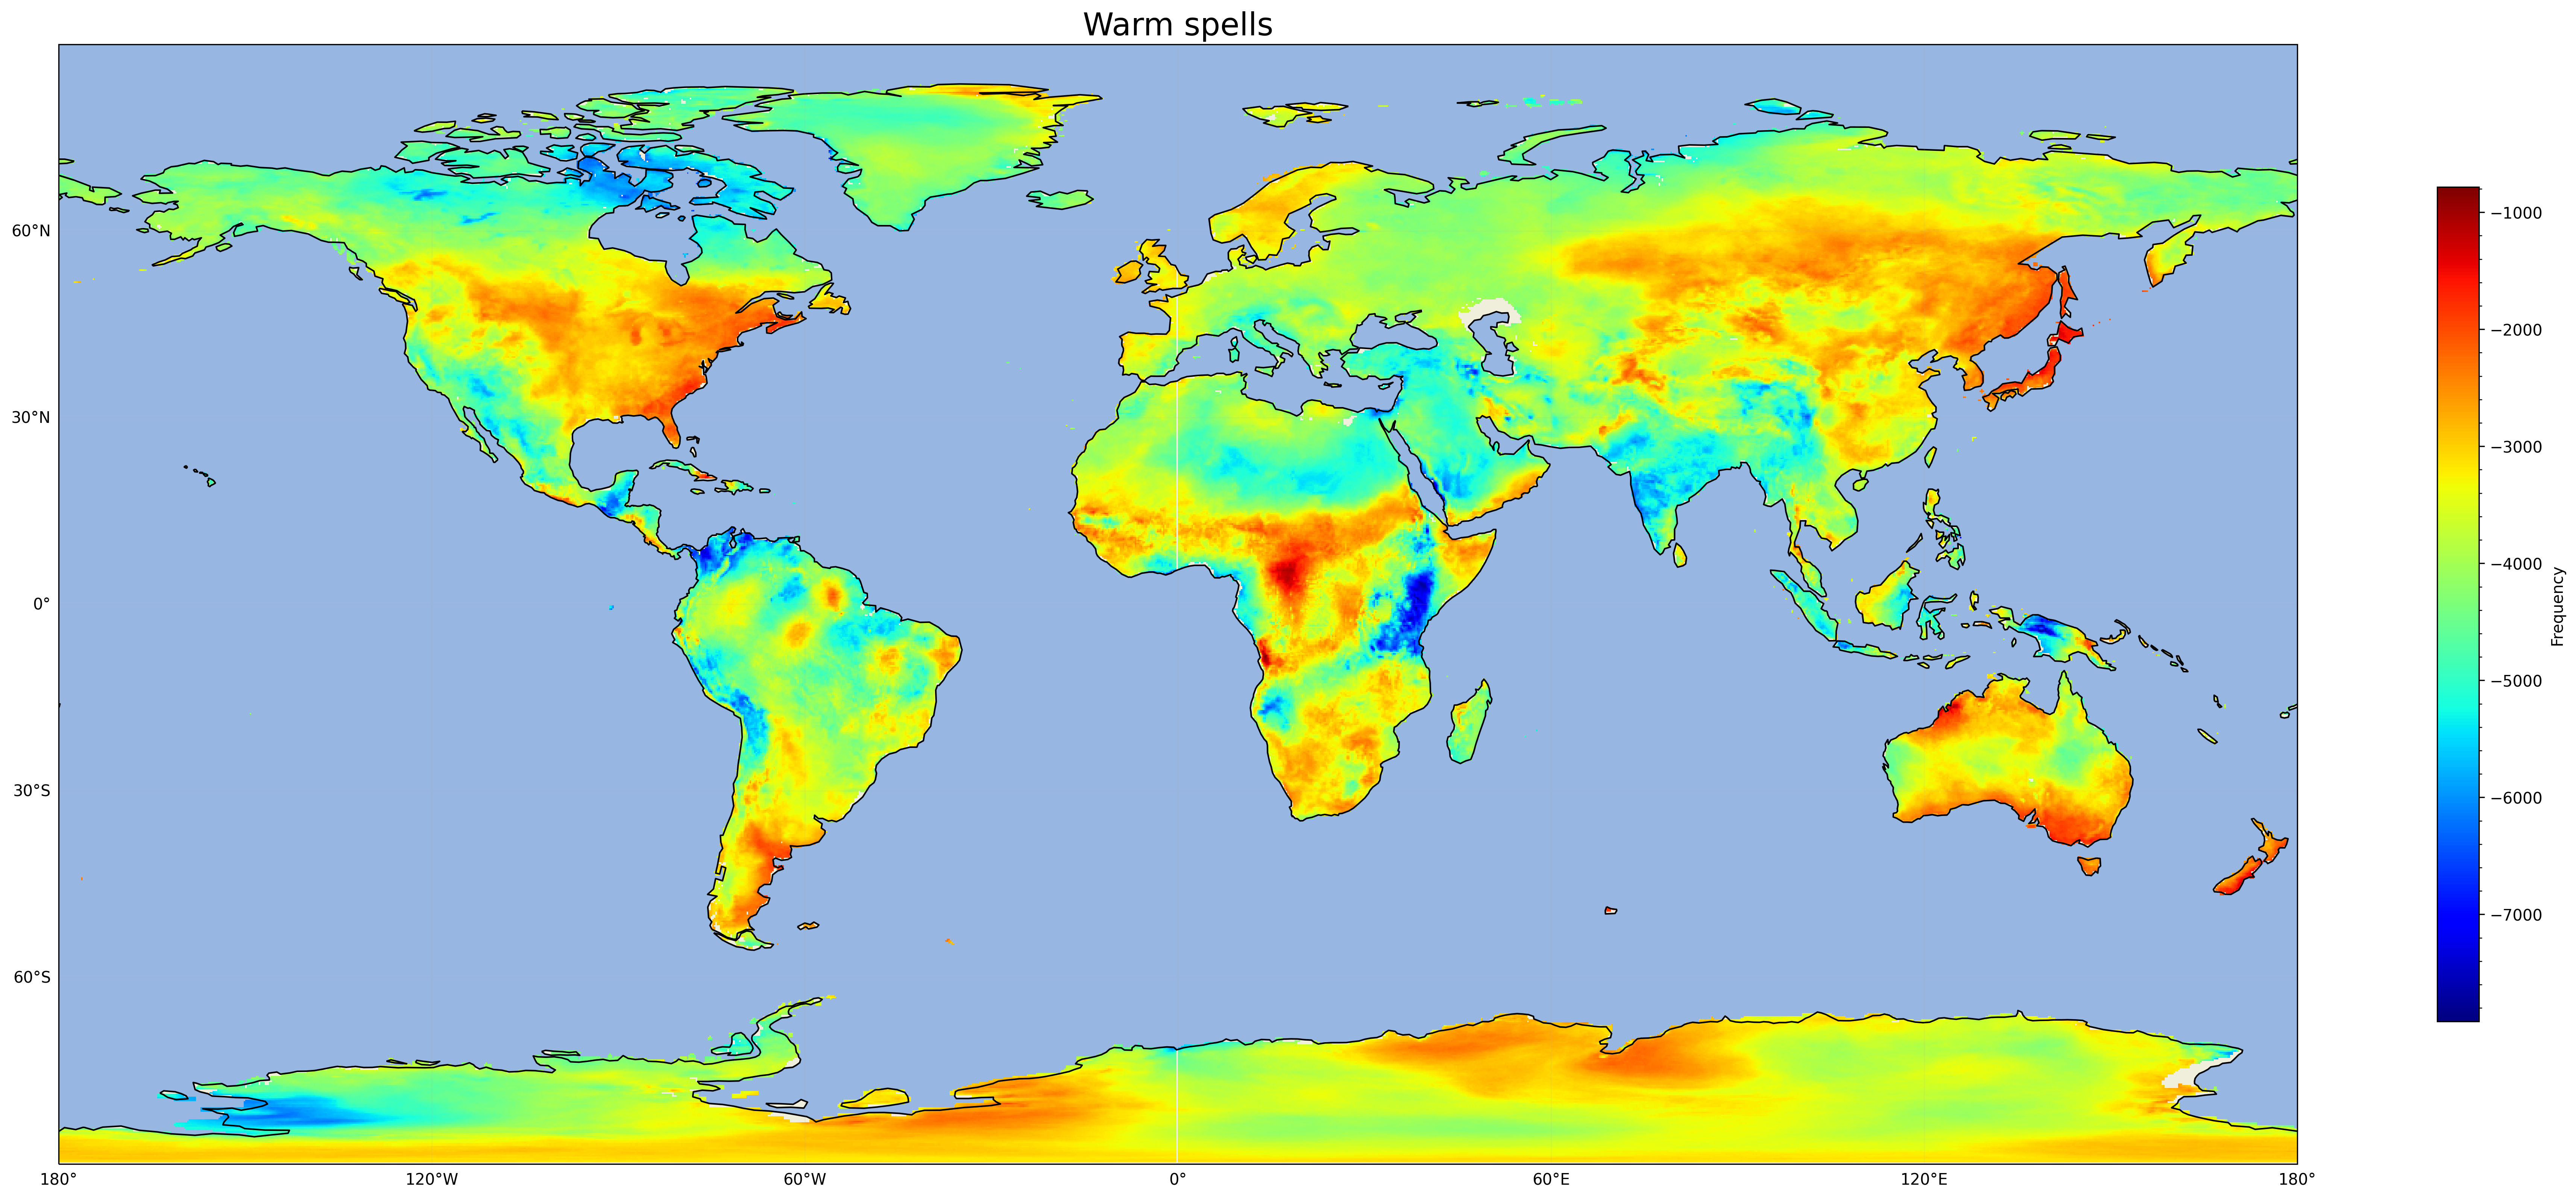
\includegraphics[width=0.80\textwidth]{/home/shiv/Documents/GitHub/EES405/clim_indices/final_plots/warmspells.png}
    \caption{Warmspells Spatial Plot}
    \label{fig:warm_spells_spatial}
\end{figure}

\subsection{Temporal Plot for 'Warm Spells (HWFI)'}
In the above time series plot of warm spells anomalies calculated from the \textbf{HWFI} climate index, we have added a non-linear trendline with polynomial fit of degree 21 (as used in the paper by )given by the following equation. \\
\begin{figure}[htb]
    \centering
    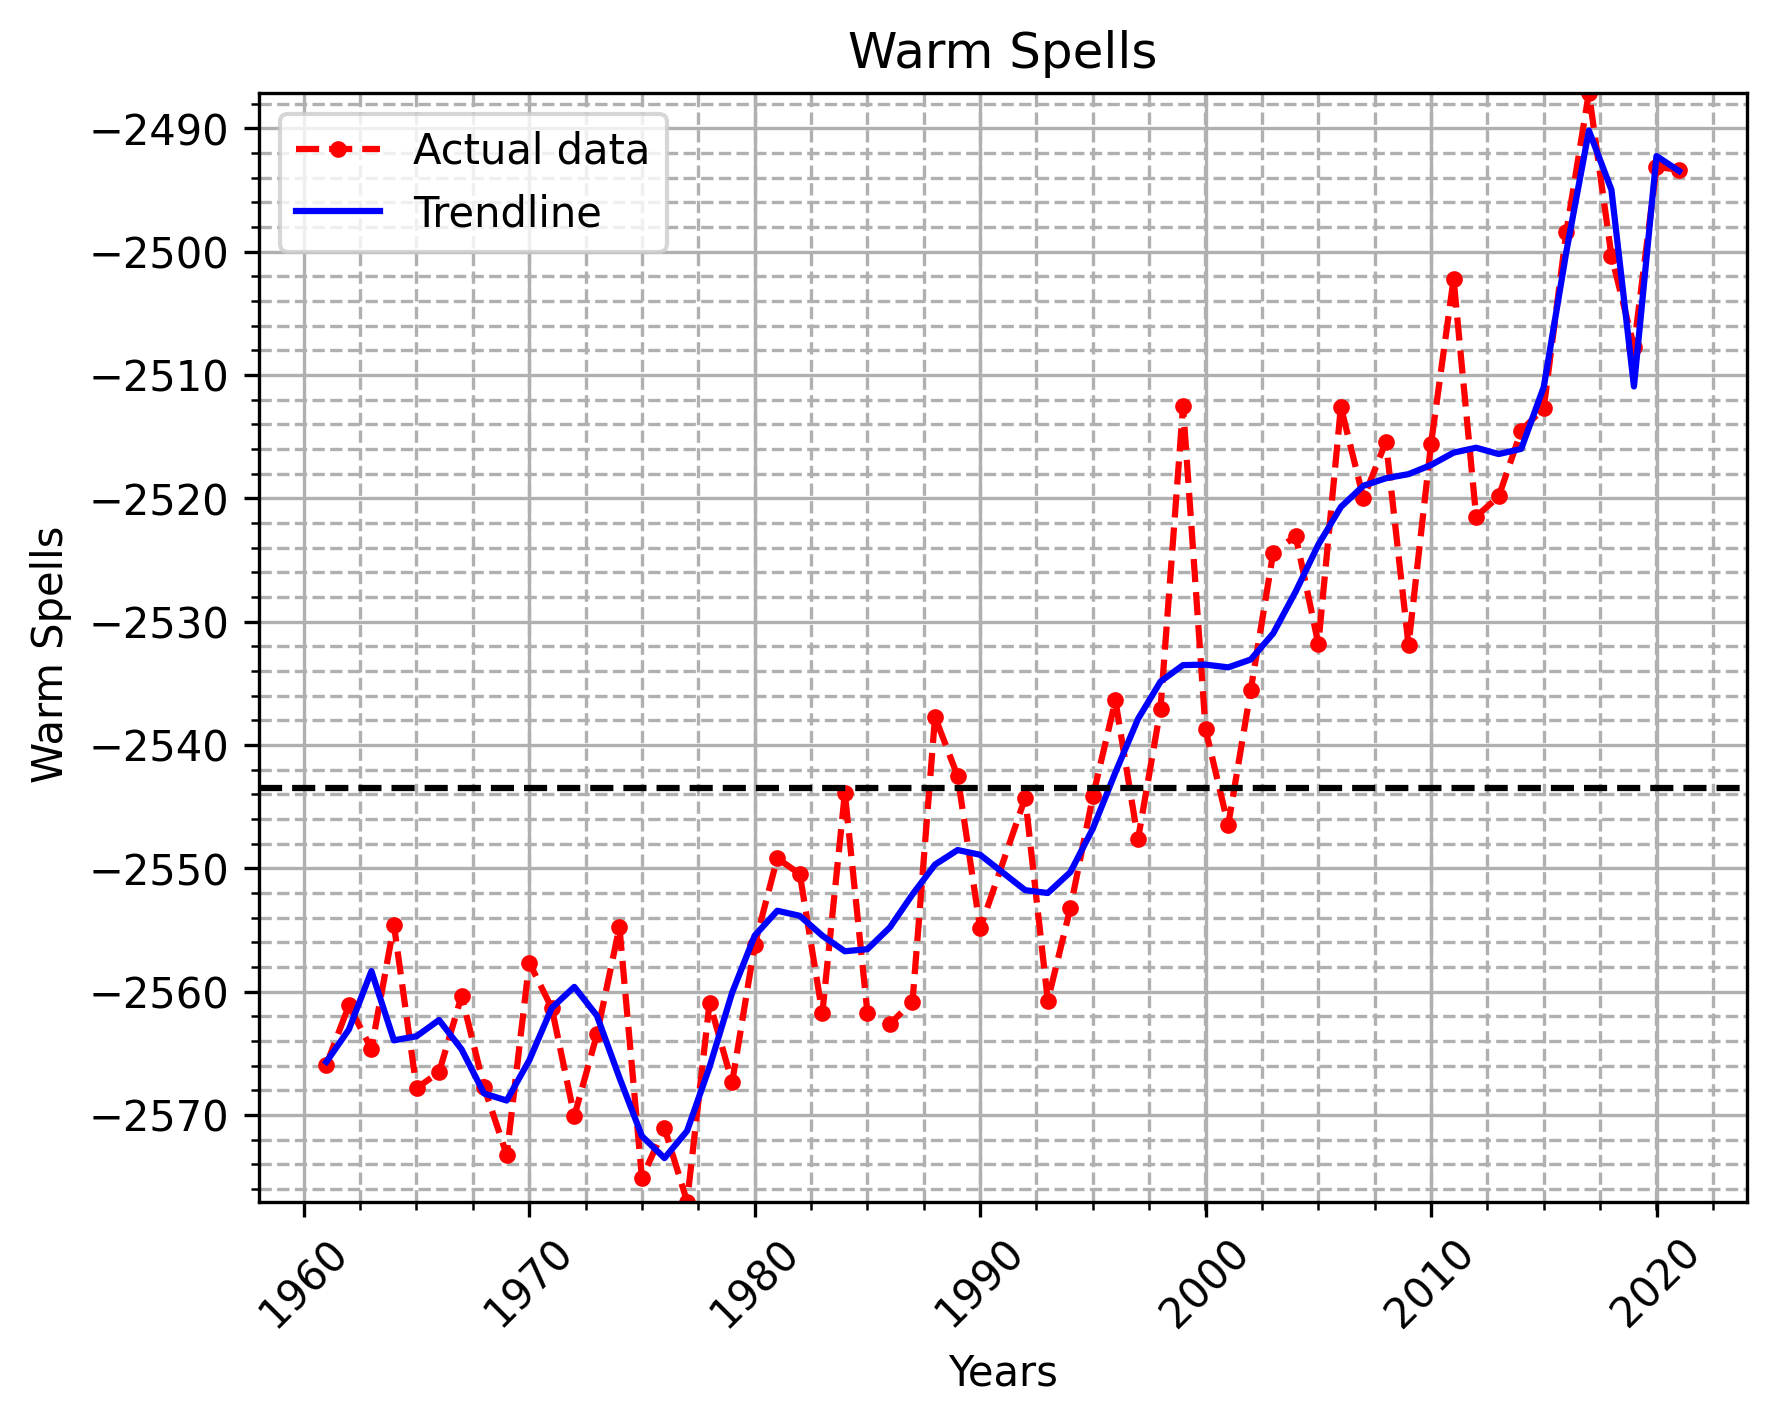
\includegraphics[width=0.75\textwidth]{/home/shiv/Documents/GitHub/EES405/clim_indices/final_plots/warmspells-timeseries.png}
    \caption{Warm spells temporal Plot}
    \label{fig:warmspells_temporal}
\end{figure}

$ y = 2.57\times10^{3}x^{21}+1.21\times10^{-2}x^{20}+3.90\times10^{-6}x^{19}-1.39\times10^{-8}x^{18}-1.46\times10^{-12}x^{17}+4.92\times10^{-15}x^{16}-3.86\times10^{-19}x^{15}-7.24\times10^{-22}x^{14}+1.83\times10^{-25}x^{13}+2.79\times10^{-29}x^{12}-1.85\times10^{-32}x^{11}+2.48\times10^{-36}x^{10}+2.42\times10^{-40}x^{9}-1.38\times10^{-43}x^{8}+2.47\times10^{-47}x^{7}-2.66\times10^{-51}x^{6}+1.94\times10^{-55}x^{5}-9.87\times10^{-60}x^{4}+3.46\times10^{-64}x^{3}-8.01\times10^{-69}x^{2}+1.11\times10^{-73}x-6.91\times10^{-79}$

The increase in the frequency of warmspells is consistent with the overall warming of the planet due to climate change as seen in the above spatial plot.\\
Overall, the increase in the frequency of warmspells is a consistent and expected result of the overall warming of the planet due to climate change.

\section{Frost Days}
\newpage
\subsection{Spatial plot for 'Frost Days (FD)'}


\begin{figure}[htb]
    \centering
    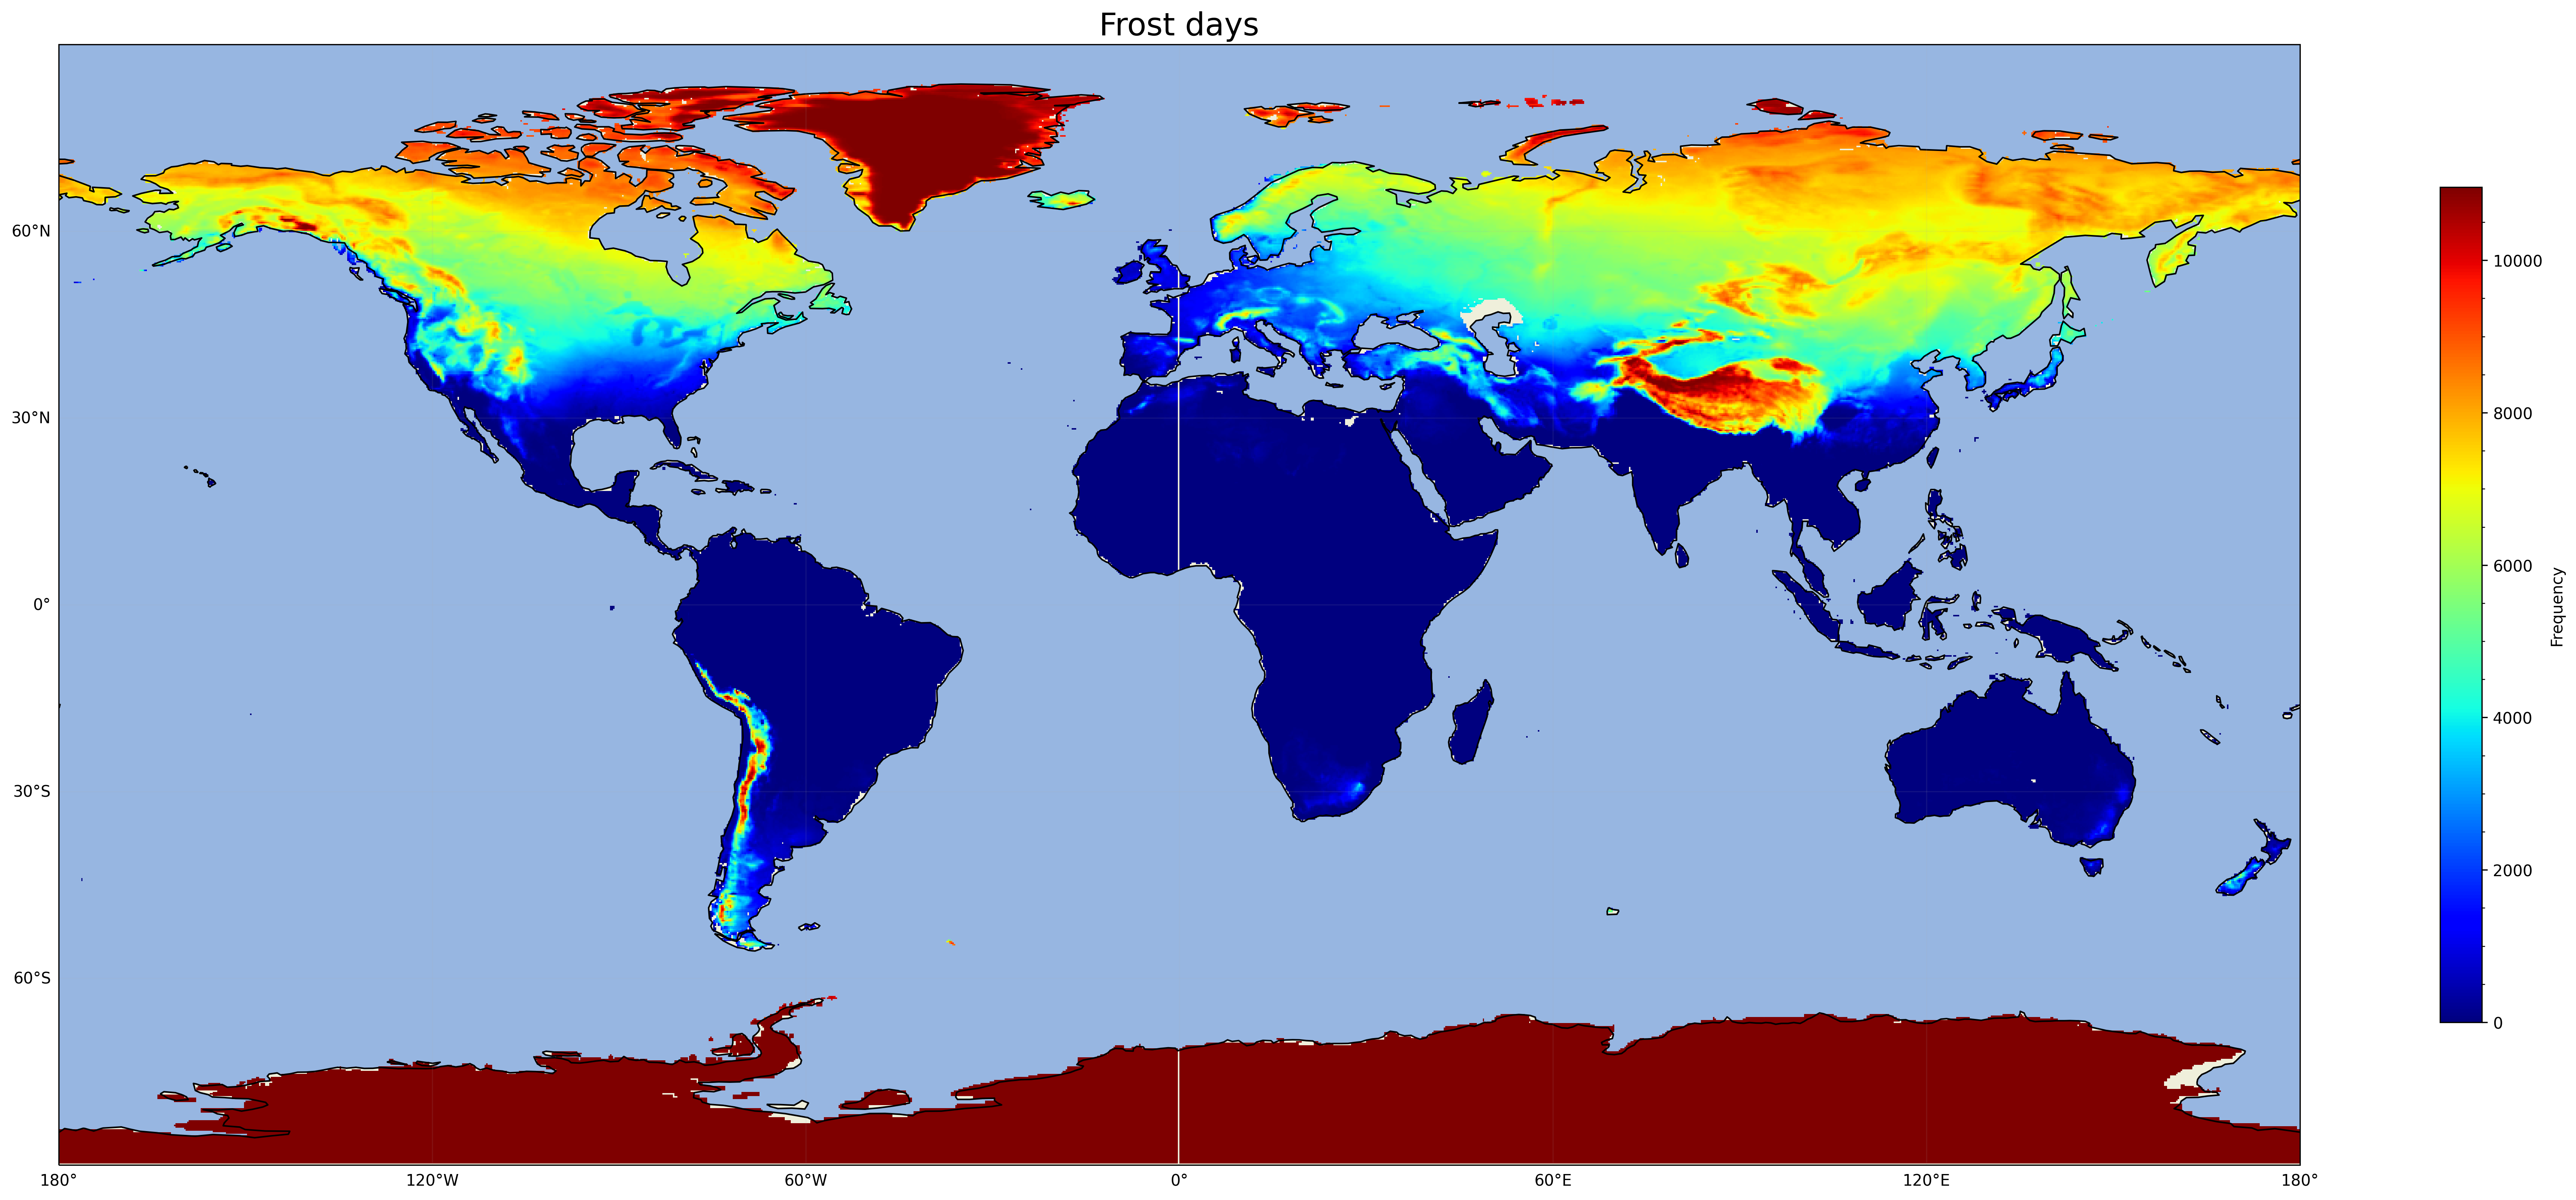
\includegraphics[width=0.80\textwidth]{/home/shiv/Documents/GitHub/EES405/clim_indices/final_plots/frostdays.png}
    \caption{Frost days Spatial Plot}
    \label{fig:frost_spatial}
\end{figure}

\subsection{Temporal Plot for 'Frost Days (FD)'}
In the above time series plot of frost days anomalies calculated from the \textbf{FD} climate index, we have added a non-linear trendline with polynomial fit of degree 21 (as used in the paper by )given by the following equation. \\
\begin{figure}[htb]
    \centering
    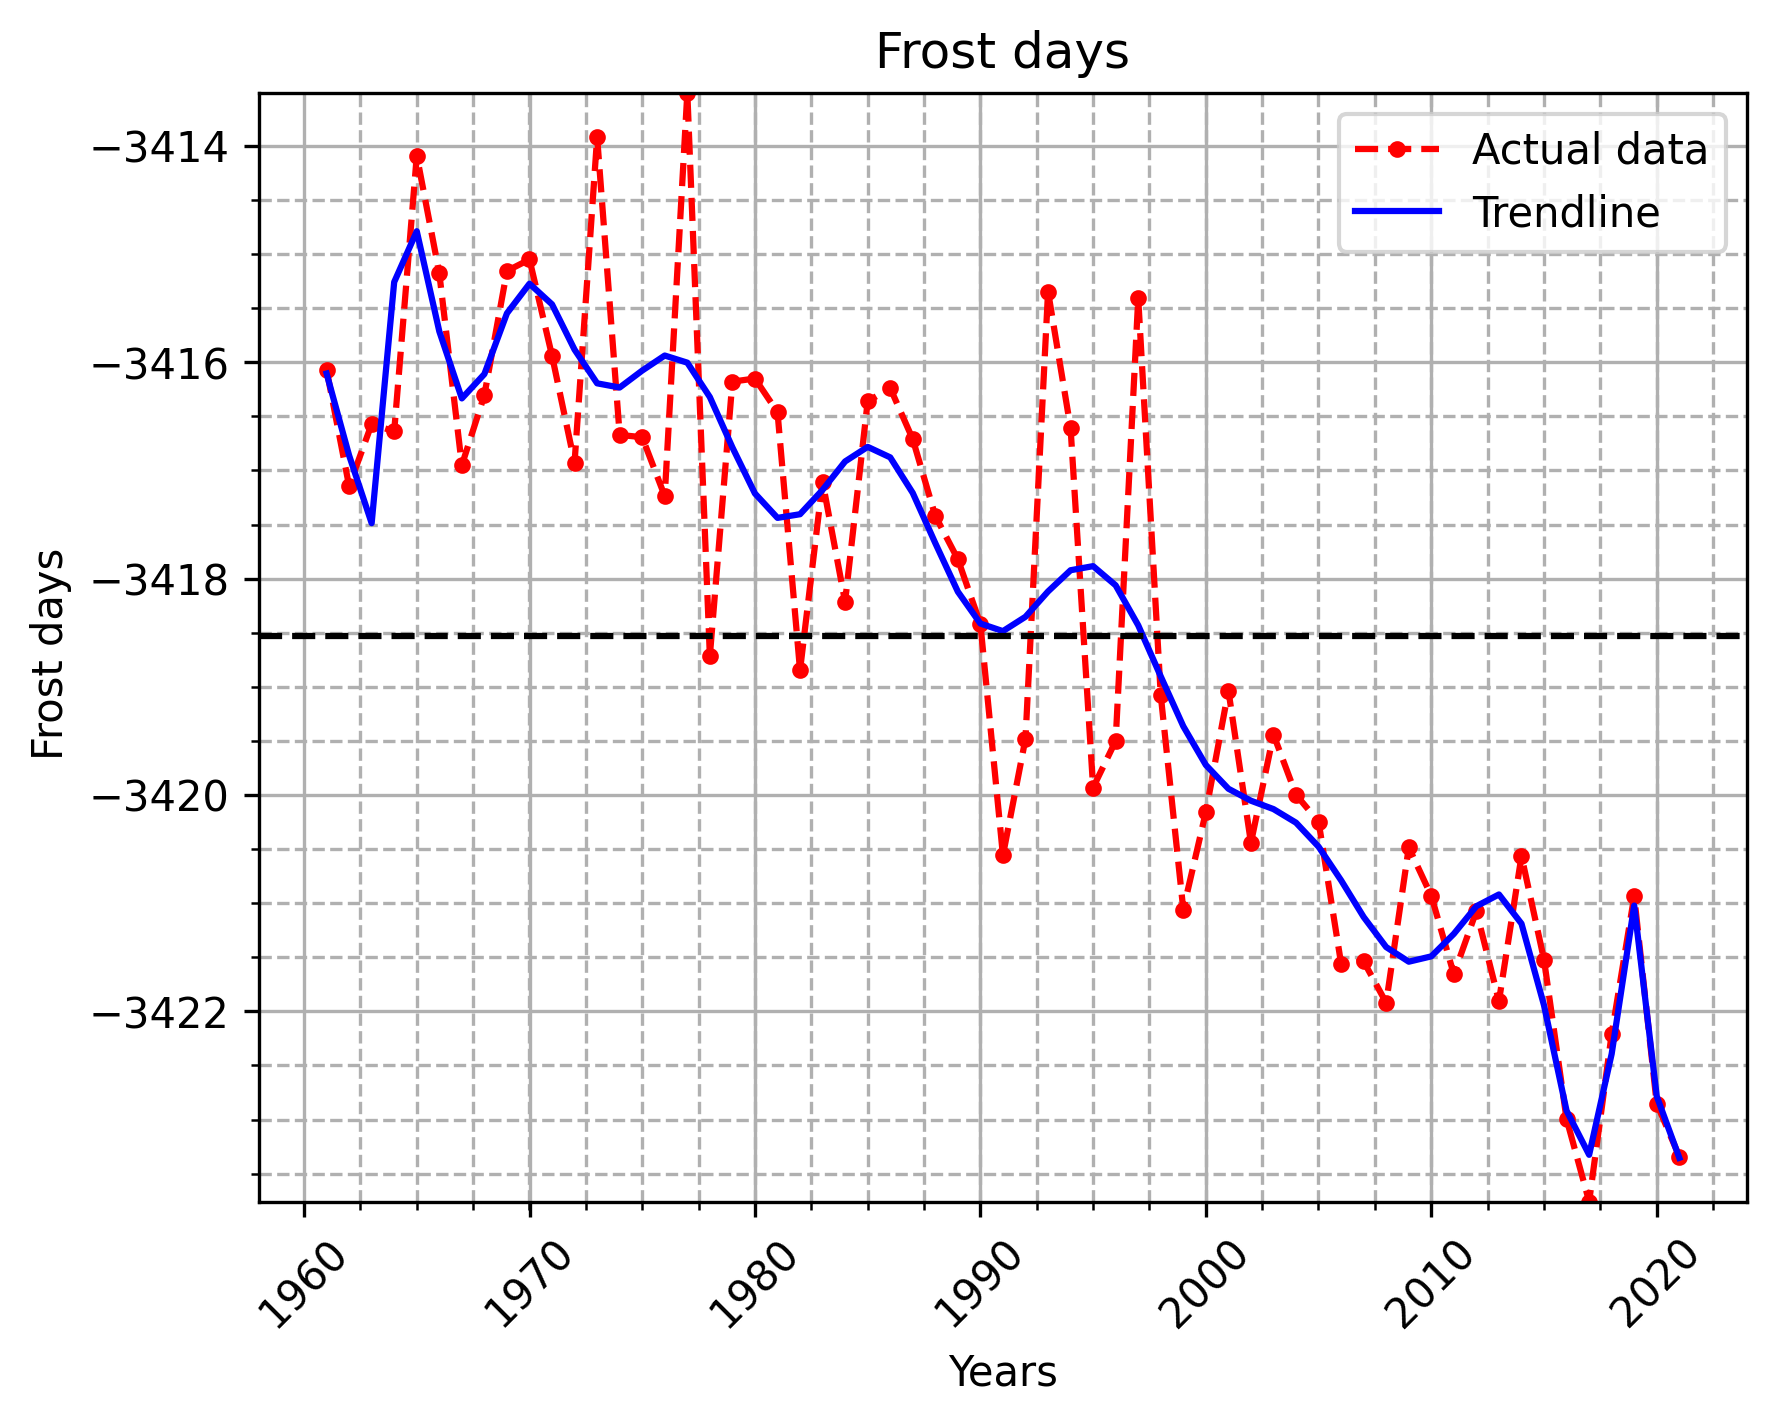
\includegraphics[width=0.75\textwidth]{/home/shiv/Documents/GitHub/EES405/clim_indices/final_plots/frost-timeseries.png}
    \caption{Frost temporal Plot}
    \label{fig:frost_temporal}
\end{figure}

$ y = -3.42\times10^{3}x^{21}+7.44\times10^{-5}x^{20}-1.88\times10^{-6}x^{19}+3.31\times10^{-10}x^{18}+1.08\times10^{-12}x^{17}-3.97\times10^{-16}x^{16}-1.62\times10^{-19}x^{15}+1.05\times10^{-22}x^{14}-5.80\times10^{-27}x^{13}-8.00\times10^{-30}x^{12}+2.29\times10^{-33}x^{11}-1.20\times10^{-37}x^{10}-6.72\times10^{-41}x^{9}+1.99\times10^{-44}x^{8}-2.95\times10^{-48}x^{7}+2.85\times10^{-52}x^{6}-1.92\times10^{-56}x^{5}+9.12\times10^{-61}x^{4}-3.03\times10^{-65}x^{3}+6.69\times10^{-70}x^{2}-8.87\times10^{-75}x+5.34\times10^{-80}$

The decrease in the frequency of frost days is consistent with the overall warming of the planet due to climate change as seen in the above spatial plot.\\
Overall, the decrease in the frequency of frost days is a consistent and expected result of the overall warming of the planet due to climate change.

\section{Extreme Temperature range}
\subsection{Spatial plot for Extreme temperature range (ETR)}
\begin{figure}[htb]
    \centering
    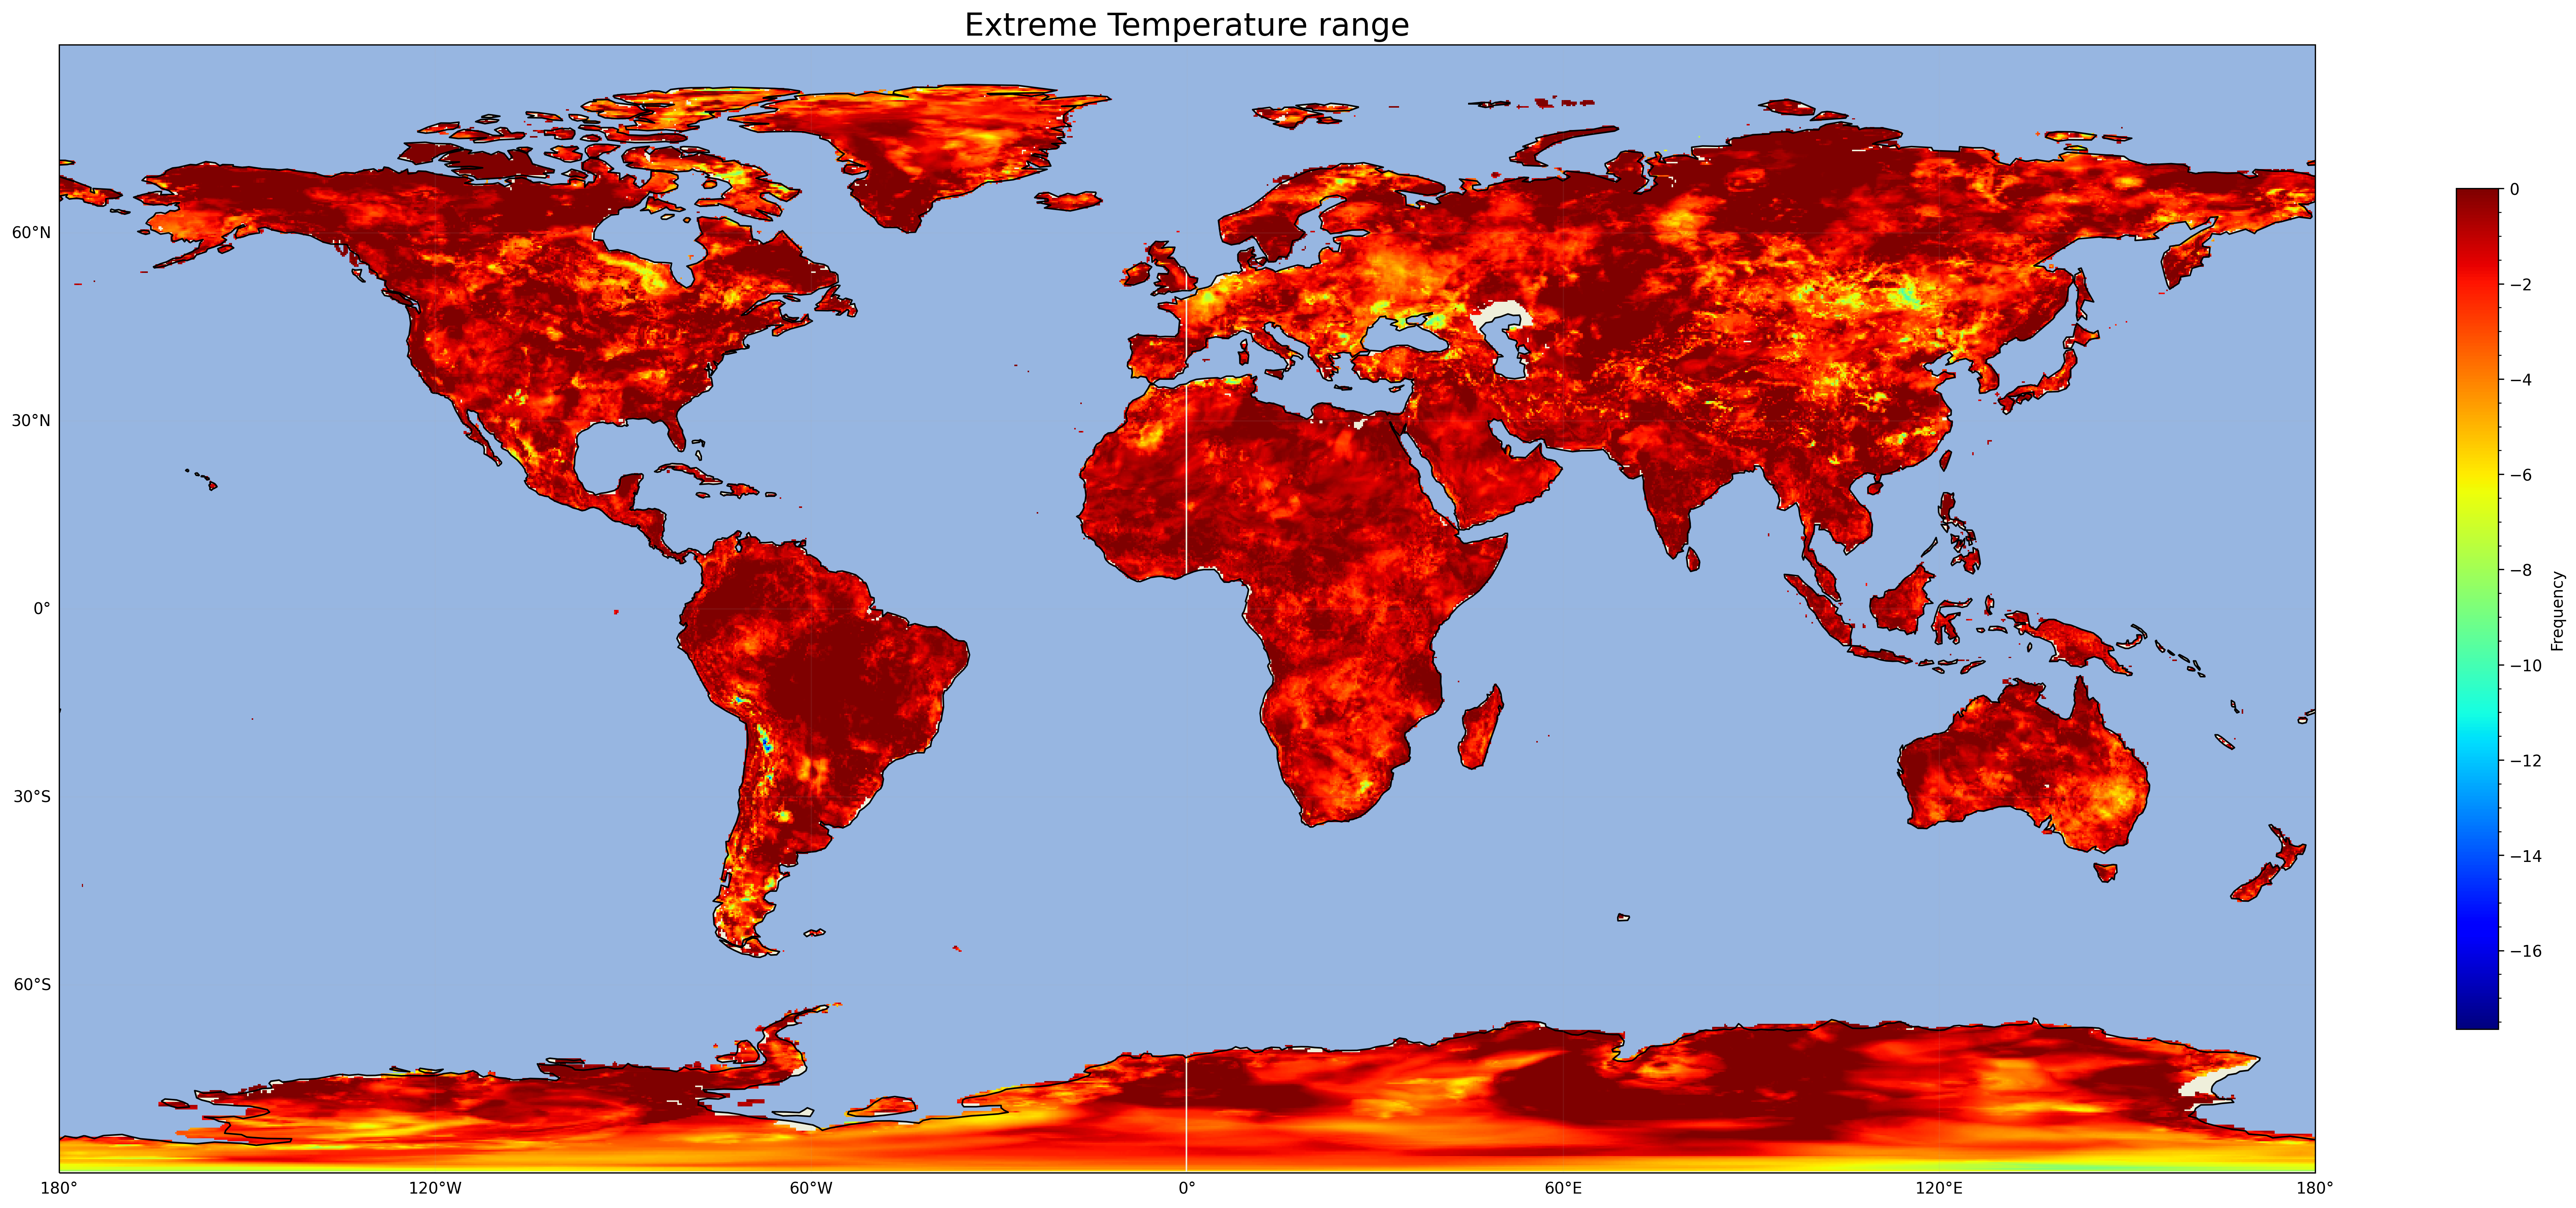
\includegraphics[width=0.80\textwidth]{/home/shiv/Documents/GitHub/EES405/clim_indices/final_plots/etr.png}
    \caption{ETR Spatial Plot}
    \label{fig:etr_spatial}
\end{figure}

\subsection{Temporal Plot for 'Extreme Temperature range (ETR)'}
In the above time series plot of Extreme Temperature range anomalies calculated from the \textbf{ETR} climate index, we have added a non-linear trendline with polynomial fit of degree 21 (as used in the paper by )given by the following equation. \\
\begin{figure}[htb]
    \centering
    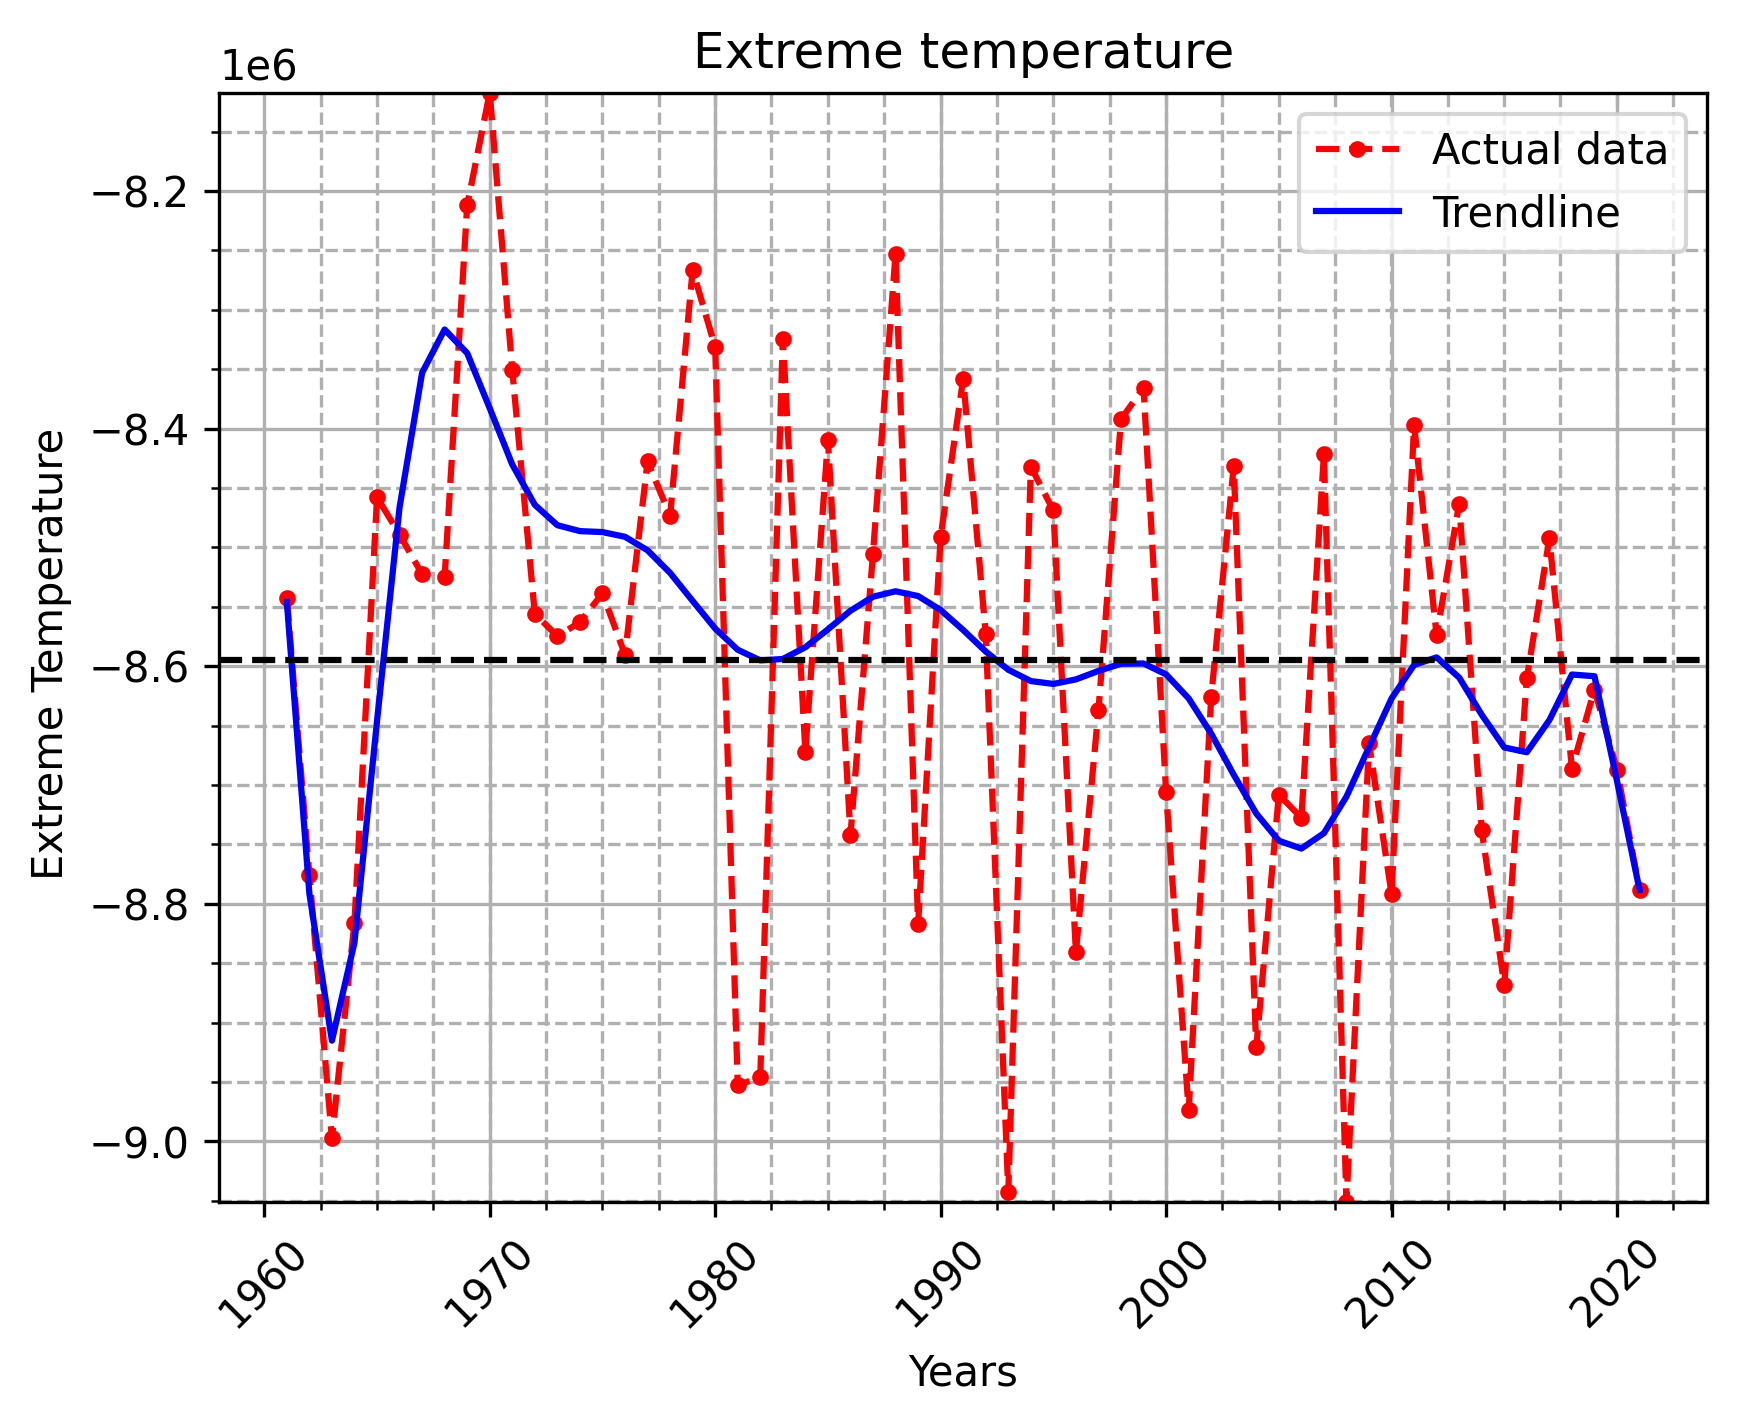
\includegraphics[width=0.75\textwidth]{//home/shiv/Documents/GitHub/EES405/clim_indices/final_plots/etr-timeseries.png}
    \caption{ETR temporal Plot}
    \label{fig:etr_temporal}
\end{figure}

$ y = -3.42\times10^{3}x^{21}+7.44\times10^{-5}x^{20}-1.88\times10^{-6}x^{19}+3.31\times10^{-10}x^{18}+1.08\times10^{-12}x^{17}-3.97\times10^{-16}x^{16}-1.62\times10^{-19}x^{15}+1.05\times10^{-22}x^{14}-5.80\times10^{-27}x^{13}-8.00\times10^{-30}x^{12}+2.29\times10^{-33}x^{11}-1.20\times10^{-37}x^{10}-6.72\times10^{-41}x^{9}+1.99\times10^{-44}x^{8}-2.95\times10^{-48}x^{7}+2.85\times10^{-52}x^{6}-1.92\times10^{-56}x^{5}+9.12\times10^{-61}x^{4}-3.03\times10^{-65}x^{3}+6.69\times10^{-70}x^{2}-8.87\times10^{-75}x+5.34\times10^{-80}$

The decrease in the frequency of frost days is consistent with the overall warming of the planet due to climate change as seen in the above spatial plot.\\
Overall, the decrease in the frequency of frost days is a consistent and expected result of the overall warming of the planet due to climate change.

\section{Seasonal occurrence of cold nights (TN10p)}
\subsection{Spatial plot for cold nights (TN10p) for DJF season }
\begin{figure}[htb]
    \centering
    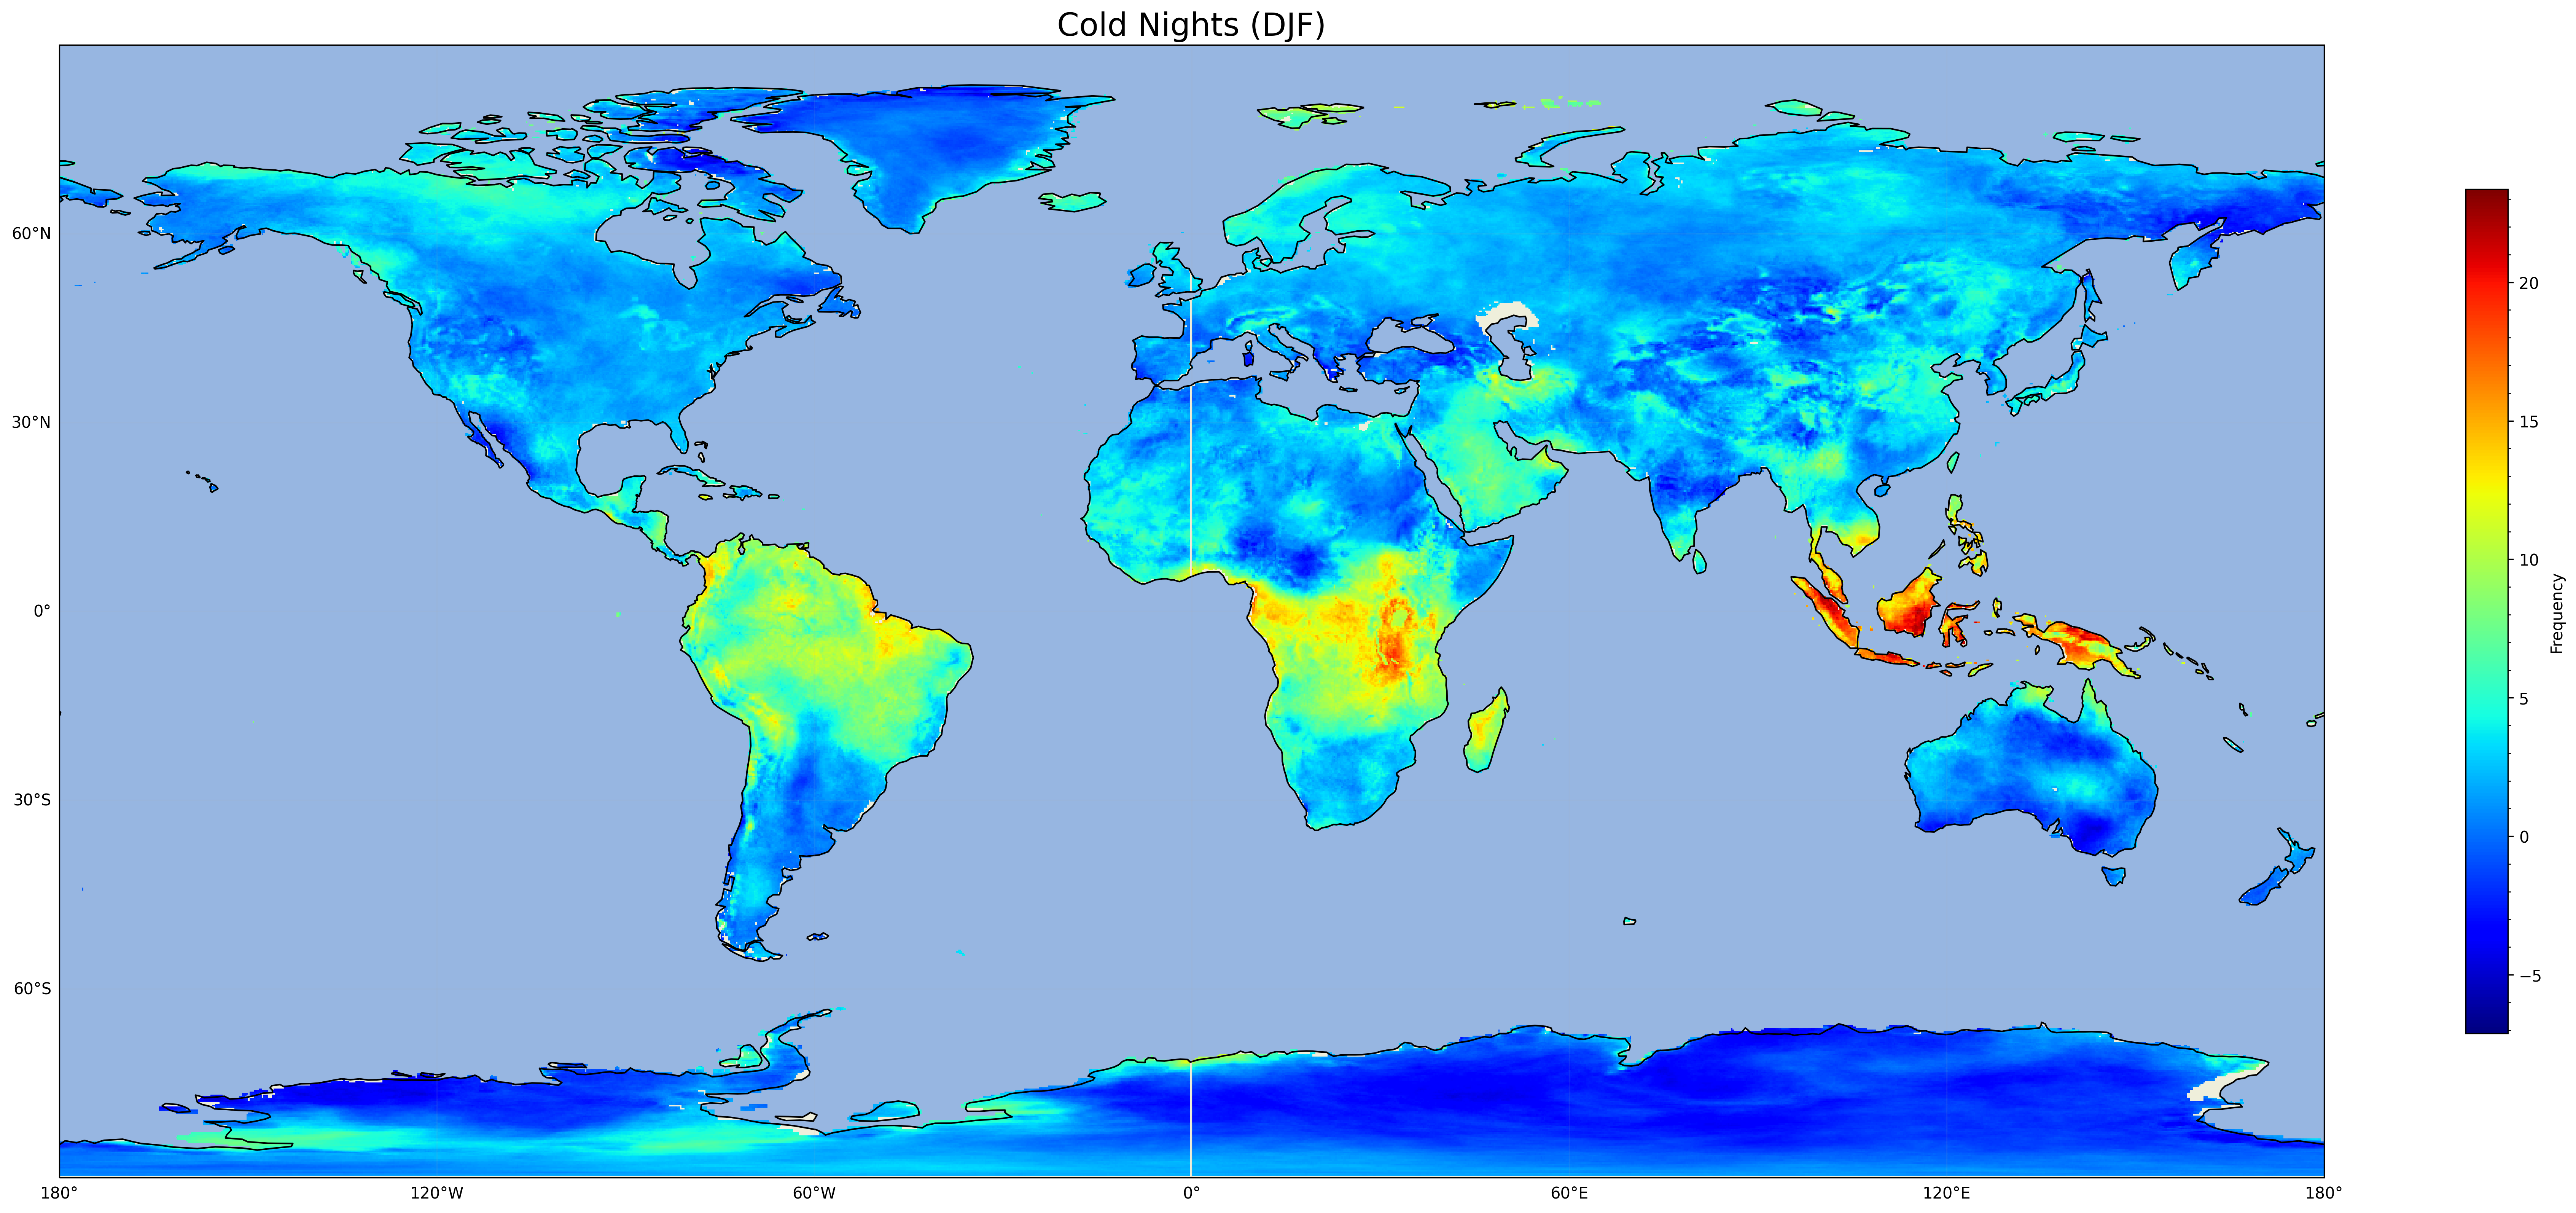
\includegraphics[width=0.80\textwidth]{/home/shiv/Documents/GitHub/EES405/clim_indices/final_plots/tn10p-djf.png}
    \caption{Cold Nights (DJF)}
    \label{fig:cold_nights_djf}
\end{figure}


\subsection{Temporal Plot for 'Seasonal occurance of cold nights (TN10p) (DJF)'}
In the above time series plot of cold night anomalies for (DJF) months calculated from the \textbf{TN10p} climate index, we have added a non-linear trendline with polynomial fit of degree 21 (as used in the paper by )given by the following equation. \\
\begin{figure}[htb]
    \centering
    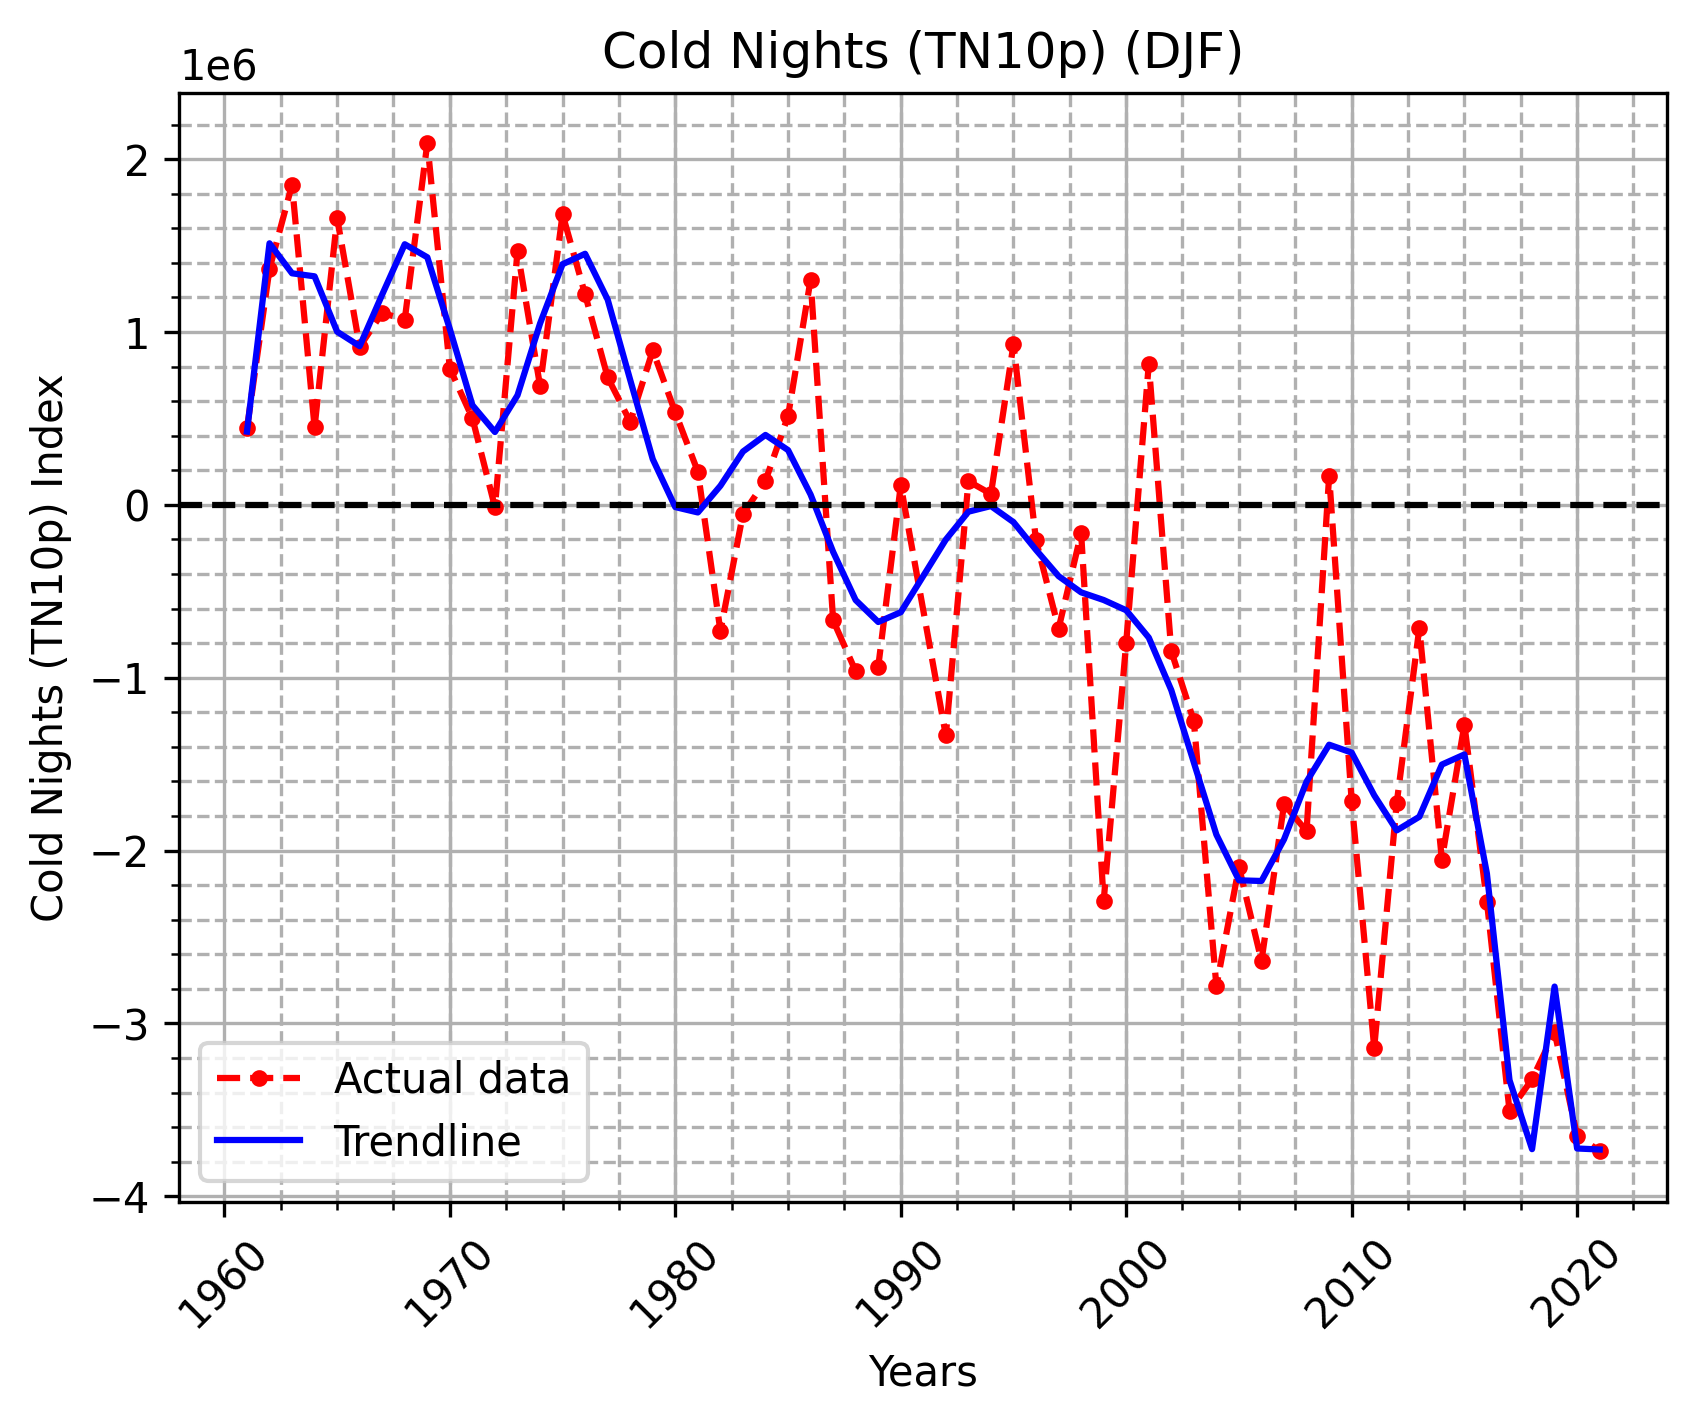
\includegraphics[width=0.75\textwidth]{/home/shiv/Documents/GitHub/EES405/clim_indices/final_plots/cold_nights_djf_timeseries.png}
    \caption{Cold Nights (TN10p) (DJF) temporal Plot}
    \label{fig:tn10p_djf_temporal}
\end{figure}

$ y = -3.42\times10^{3}x^{21}+7.44\times10^{-5}x^{20}-1.88\times10^{-6}x^{19}+3.31\times10^{-10}x^{18}+1.08\times10^{-12}x^{17}-3.97\times10^{-16}x^{16}-1.62\times10^{-19}x^{15}+1.05\times10^{-22}x^{14}-5.80\times10^{-27}x^{13}-8.00\times10^{-30}x^{12}+2.29\times10^{-33}x^{11}-1.20\times10^{-37}x^{10}-6.72\times10^{-41}x^{9}+1.99\times10^{-44}x^{8}-2.95\times10^{-48}x^{7}+2.85\times10^{-52}x^{6}-1.92\times10^{-56}x^{5}+9.12\times10^{-61}x^{4}-3.03\times10^{-65}x^{3}+6.69\times10^{-70}x^{2}-8.87\times10^{-75}x+5.34\times10^{-80}$

The decrease in the frequency of cold nights is consistent with the overall warming of the planet due to climate change as seen in the above spatial plot.\\
Overall, the decrease in the frequency of cold nights is a consistent and expected result of the overall warming of the planet due to climate change.

\newpage
\subsection{Spatial plot for cold nights (TN10p) for MAM season}

\begin{figure}[htb]
    \centering
    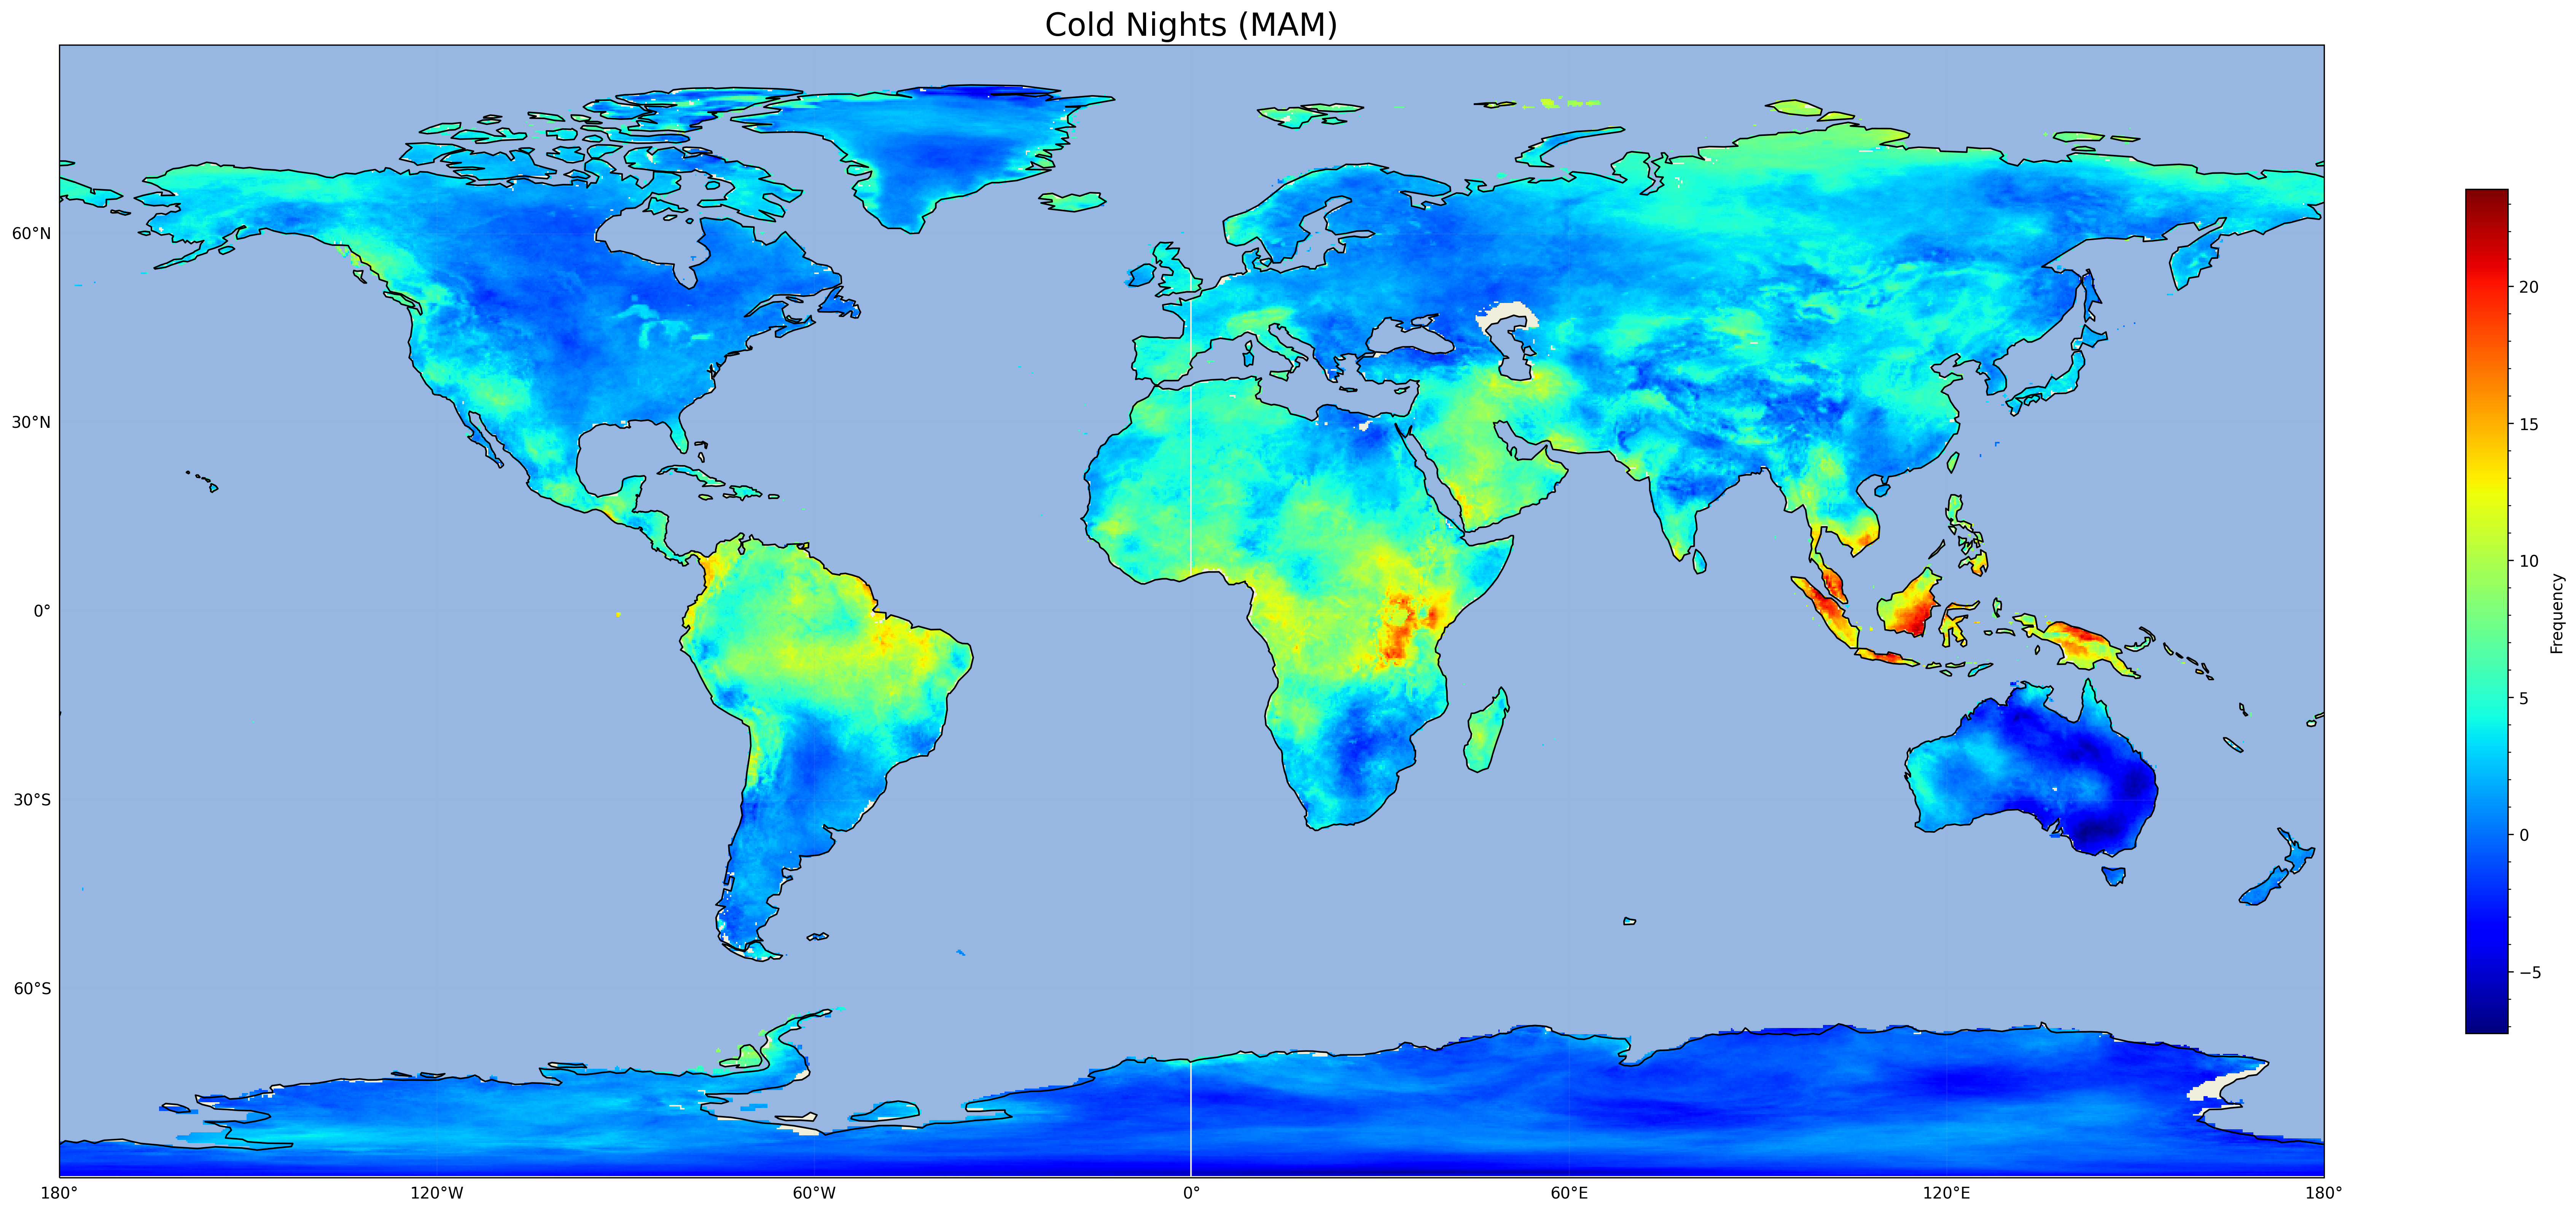
\includegraphics[width=0.80\textwidth]{/home/shiv/Documents/GitHub/EES405/clim_indices/final_plots/tn10p-mam.png}
    \caption{Cold Nights MAM Spatial Plot}
    \label{fig:tn10p_mam_spatial}
\end{figure}

\subsection{Temporal Plot for 'Seasonal occurance of cold nights (TN10p) (MAM)'}
In the above time series plot of cold night anomalies for (MAM) months calculated from the \textbf{TN10p} climate index, we have added a non-linear trendline with polynomial fit of degree 21 (as used in the paper by )given by the following equation.
\begin{figure}[htb]
    \centering
    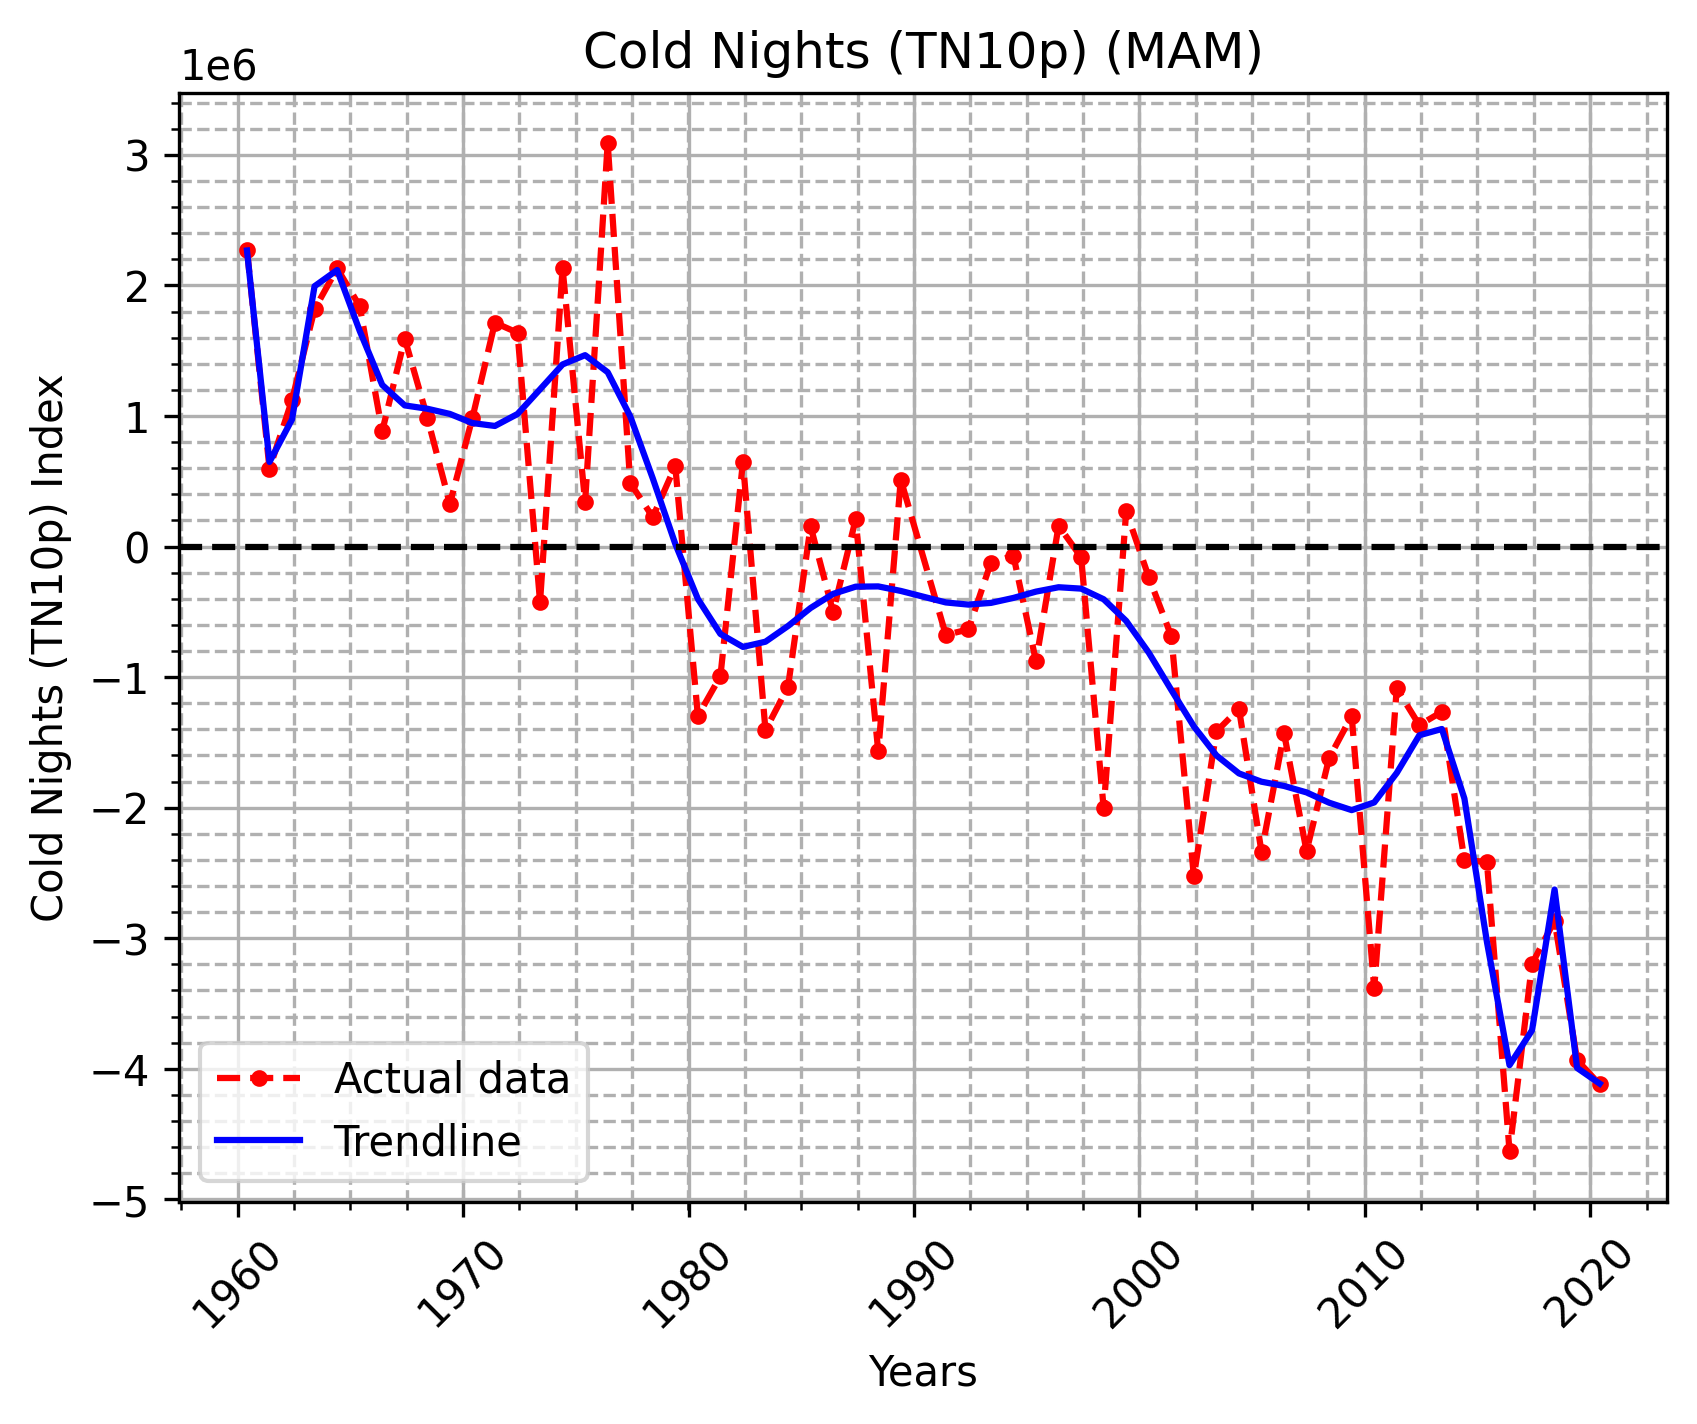
\includegraphics[width=0.75\textwidth]{//home/shiv/Documents/GitHub/EES405/clim_indices/final_plots/cold_nights_mam_timeseries.png}
    \caption{Cold Nights (TN10p) (MAM) temporal Plot}
    \label{fig:tn10p_mam_temporal}
\end{figure}

$ y = -3.42\times10^{3}x^{21}+7.44\times10^{-5}x^{20}-1.88\times10^{-6}x^{19}+3.31\times10^{-10}x^{18}+1.08\times10^{-12}x^{17}-3.97\times10^{-16}x^{16}-1.62\times10^{-19}x^{15}+1.05\times10^{-22}x^{14}-5.80\times10^{-27}x^{13}-8.00\times10^{-30}x^{12}+2.29\times10^{-33}x^{11}-1.20\times10^{-37}x^{10}-6.72\times10^{-41}x^{9}+1.99\times10^{-44}x^{8}-2.95\times10^{-48}x^{7}+2.85\times10^{-52}x^{6}-1.92\times10^{-56}x^{5}+9.12\times10^{-61}x^{4}-3.03\times10^{-65}x^{3}+6.69\times10^{-70}x^{2}-8.87\times10^{-75}x+5.34\times10^{-80}$

The decrease in the frequency of cold nights is consistent with the overall warming of the planet due to climate change as seen in the above spatial plot.\\
Overall, the decrease in the frequency of cold nights is a consistent and expected result of the overall warming of the planet due to climate change.

\subsection{Spatial plot for cold nights (TN10p) for JJA season}

\begin{figure}[htb]
    \centering
    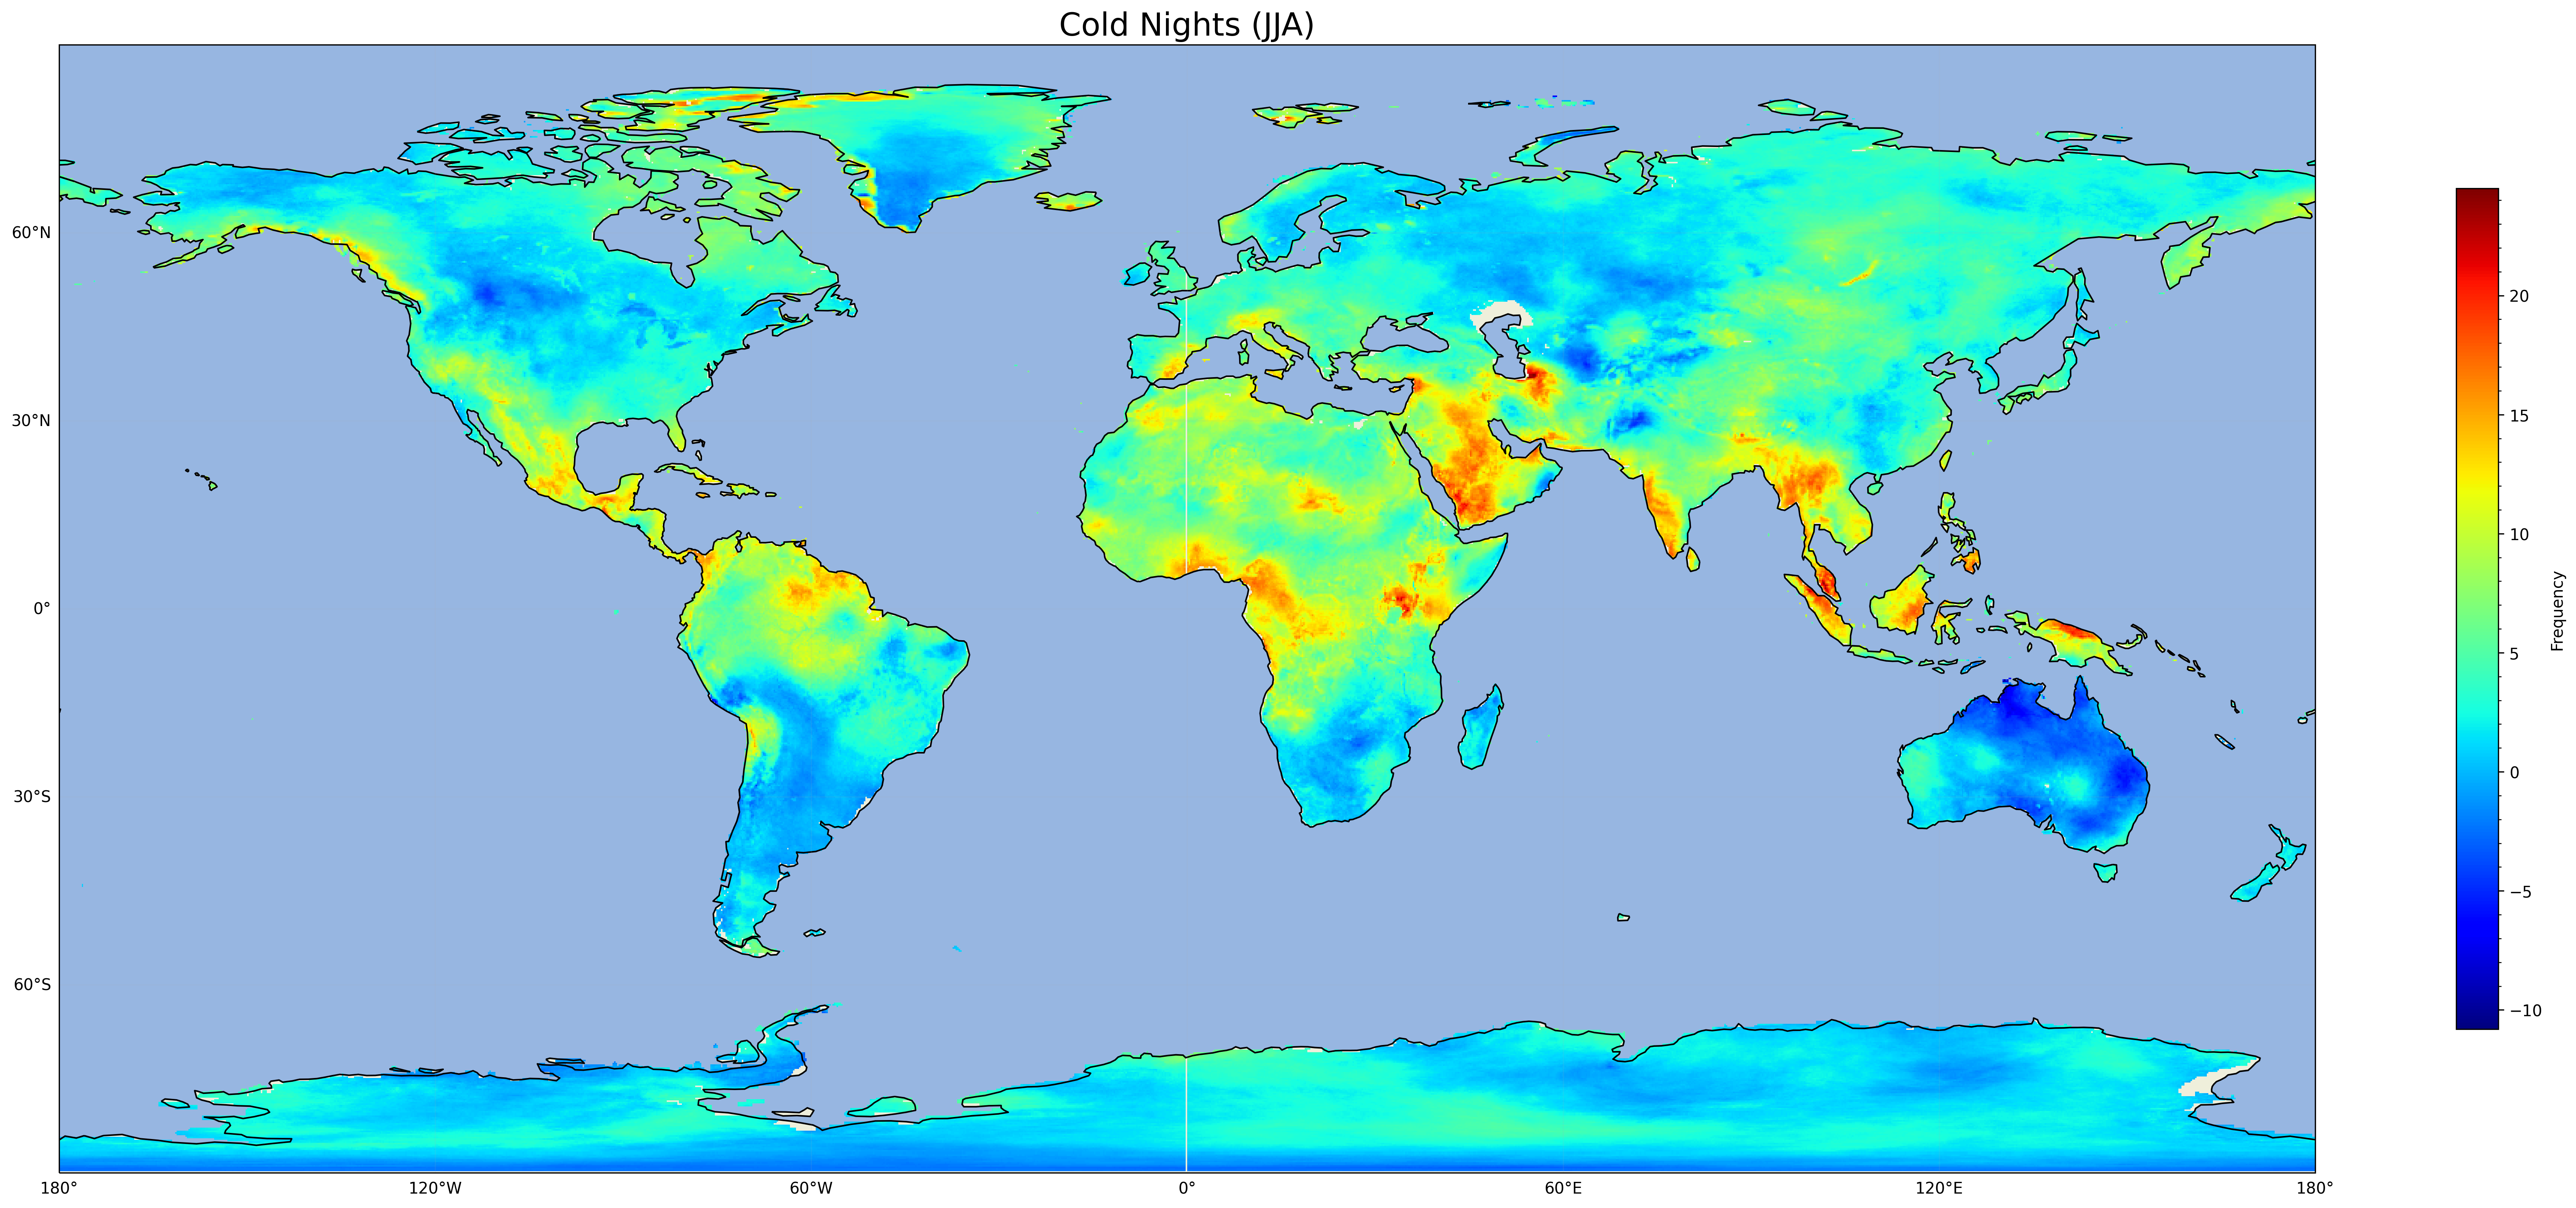
\includegraphics[width=0.80\textwidth]{/home/shiv/Documents/GitHub/EES405/clim_indices/final_plots/tn10p-jja.png}
    \caption{Cold Nights JJA Spatial Plot}
    \label{fig:tn10p_jja_spatial}
\end{figure}

\subsection{Temporal Plot for 'Seasonal occurance of cold nights (TN10p) (JJA)'}
In the above time series plot of cold night anomalies for (JJA) months calculated from the \textbf{TN10p} climate index, we have added a non-linear trendline with polynomial fit of degree 21 (as used in the paper by )given by the following equation. \\
\begin{figure}[htb]
    \centering
    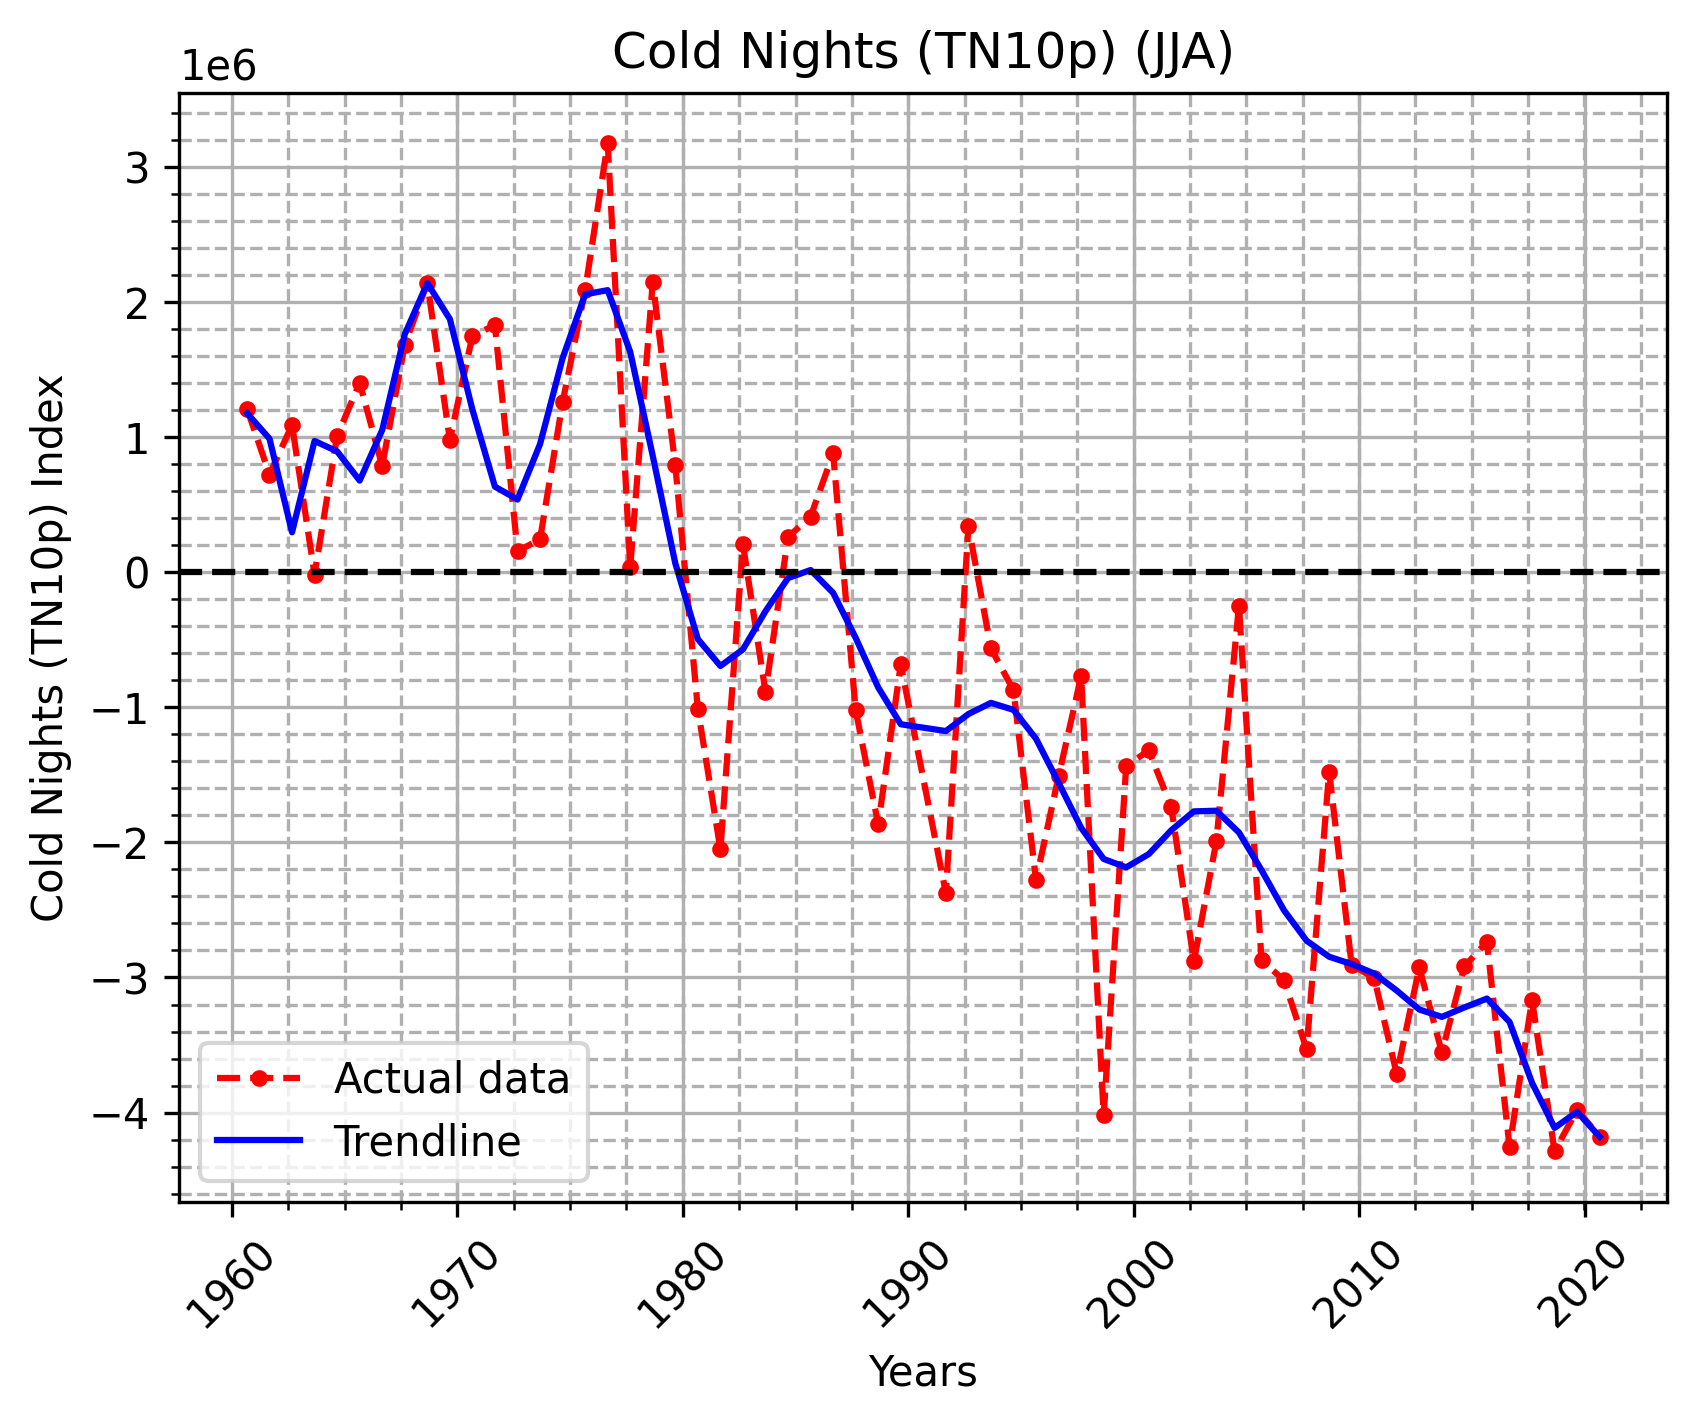
\includegraphics[width=0.75\textwidth]{//home/shiv/Documents/GitHub/EES405/clim_indices/final_plots/cold_nights_jja_timeseries.png}
    \caption{Cold Nights (TN10p) (JJA) temporal Plot}
    \label{fig:tn10p_jja_temporal}
\end{figure}

$ y = -3.42\times10^{3}x^{21}+7.44\times10^{-5}x^{20}-1.88\times10^{-6}x^{19}+3.31\times10^{-10}x^{18}+1.08\times10^{-12}x^{17}-3.97\times10^{-16}x^{16}-1.62\times10^{-19}x^{15}+1.05\times10^{-22}x^{14}-5.80\times10^{-27}x^{13}-8.00\times10^{-30}x^{12}+2.29\times10^{-33}x^{11}-1.20\times10^{-37}x^{10}-6.72\times10^{-41}x^{9}+1.99\times10^{-44}x^{8}-2.95\times10^{-48}x^{7}+2.85\times10^{-52}x^{6}-1.92\times10^{-56}x^{5}+9.12\times10^{-61}x^{4}-3.03\times10^{-65}x^{3}+6.69\times10^{-70}x^{2}-8.87\times10^{-75}x+5.34\times10^{-80}$

The decrease in the frequency of cold nights is consistent with the overall warming of the planet due to climate change as seen in the above spatial plot.\\
Overall, the decrease in the frequency of cold nights is a consistent and expected result of the overall warming of the planet due to climate change.

\subsection{Spatial plot for cold nights (TN10p) for SON season}

\begin{figure}[htb]
    \centering
    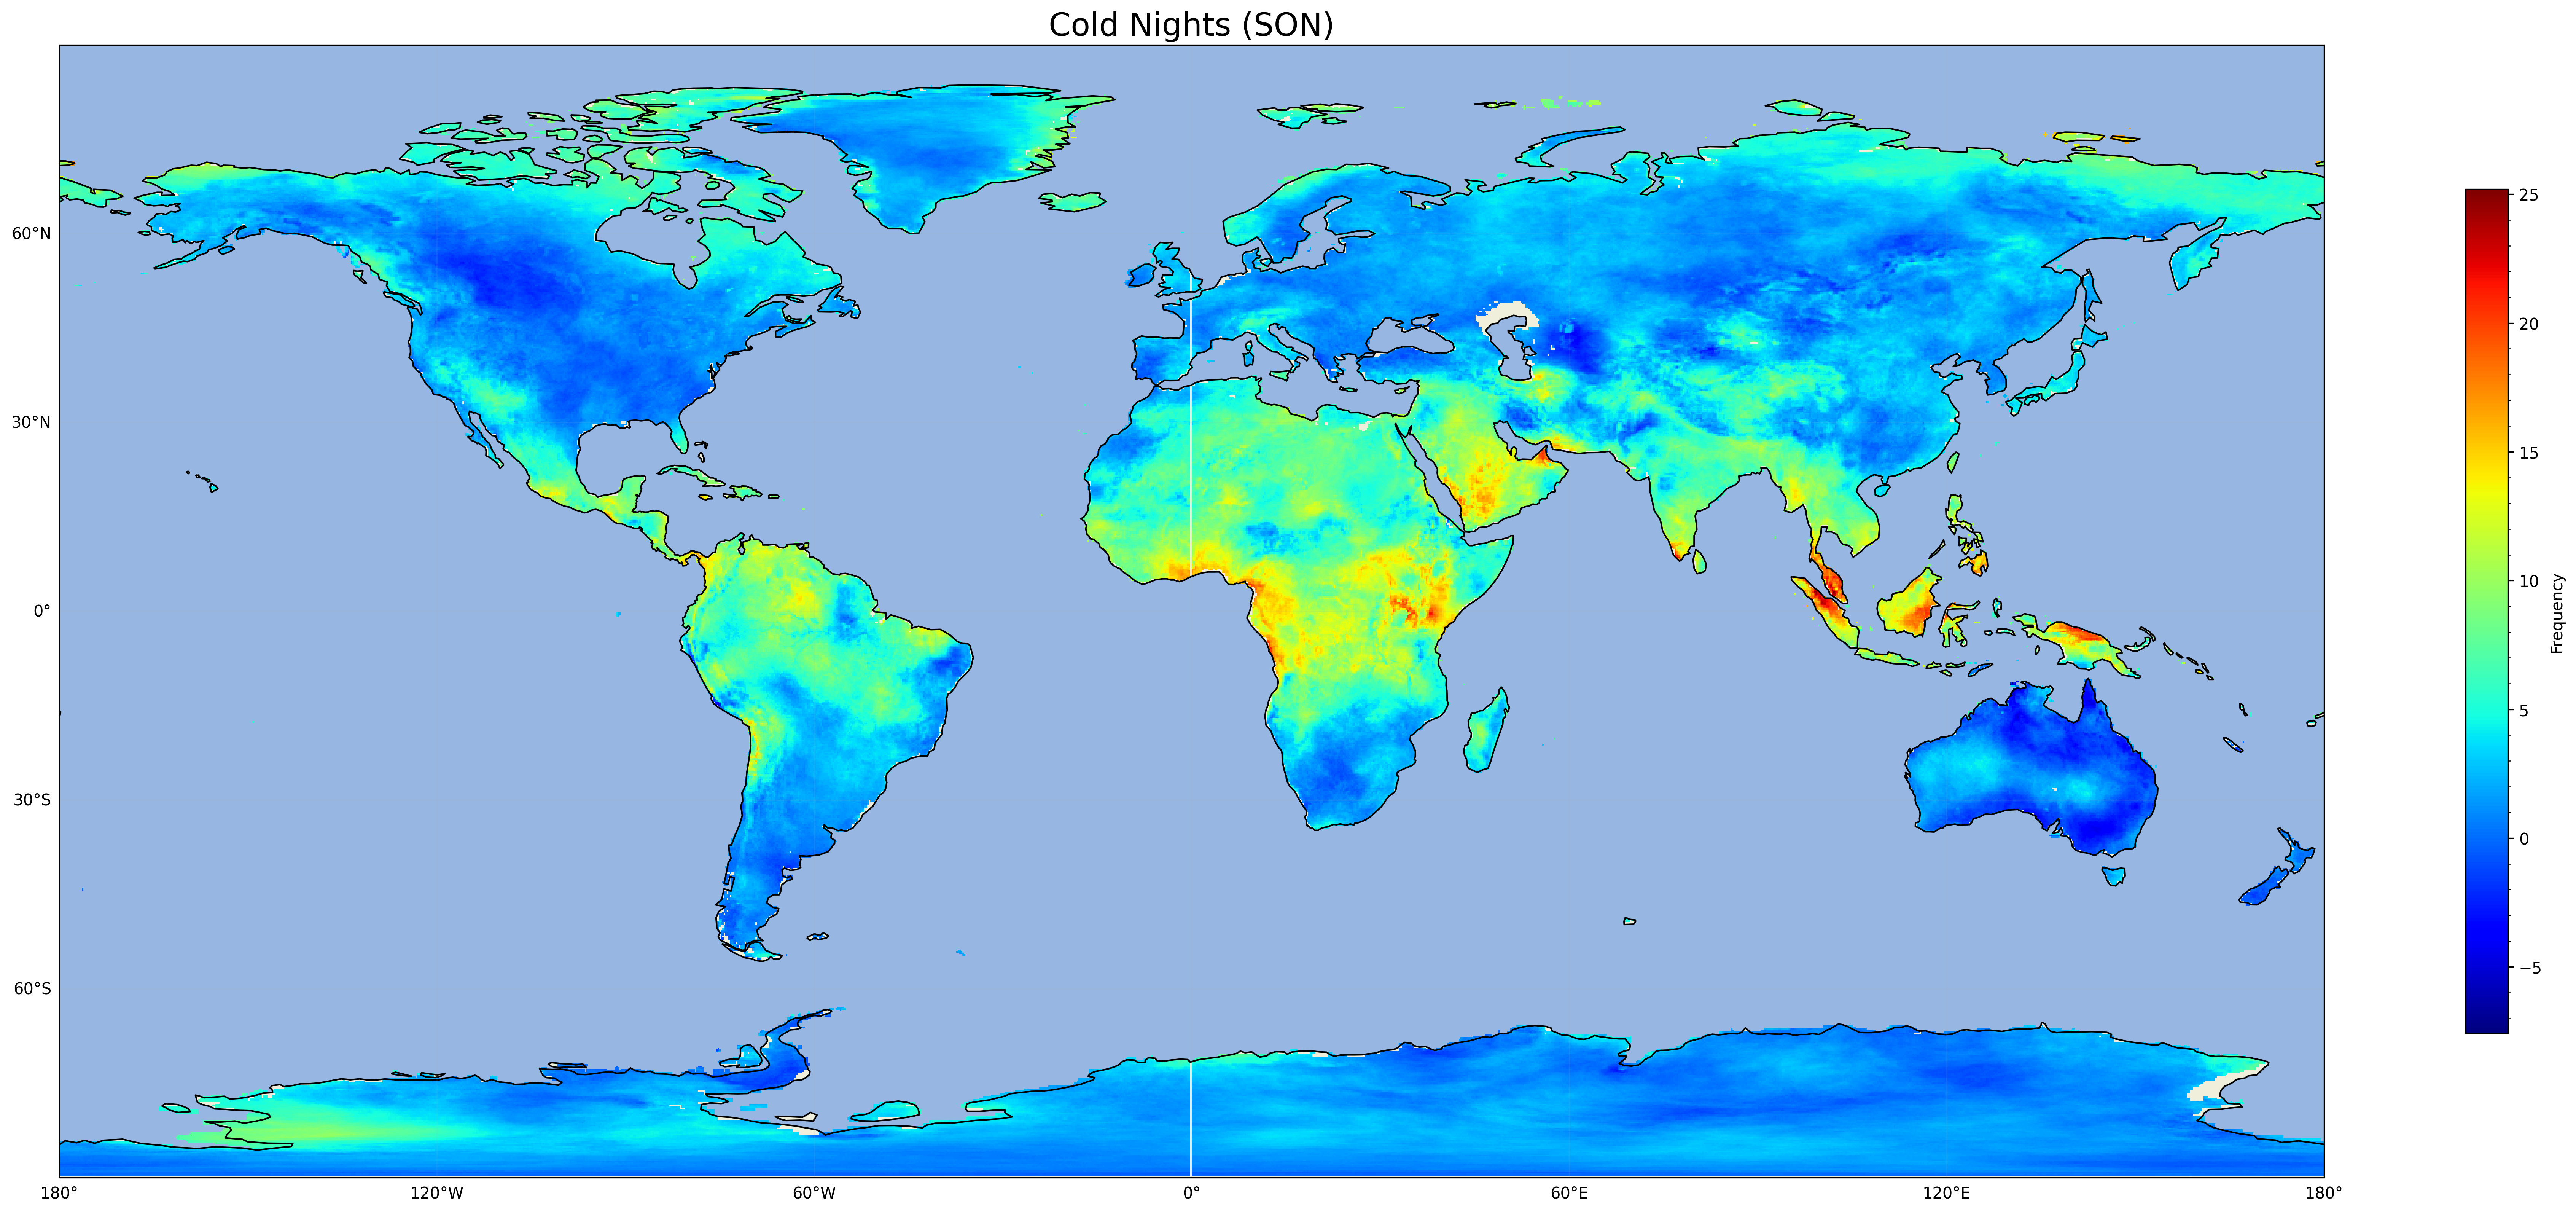
\includegraphics[width=0.80\textwidth]{/home/shiv/Documents/GitHub/EES405/clim_indices/final_plots/tn10p-son.png}
    \caption{Cold Nights SON Spatial Plot}
    \label{fig:tn10p_son_spatial}
\end{figure}

\subsection{Temporal Plot for 'Seasonal occurance of cold nights (TN10p) (SON)'}
In the above time series plot of cold night anomalies for (SON) months calculated from the \textbf{TN10p} climate index, we have added a non-linear trendline with polynomial fit of degree 21 (as used in the paper by )given by the following equation.
\begin{figure}[htb]
    \centering
    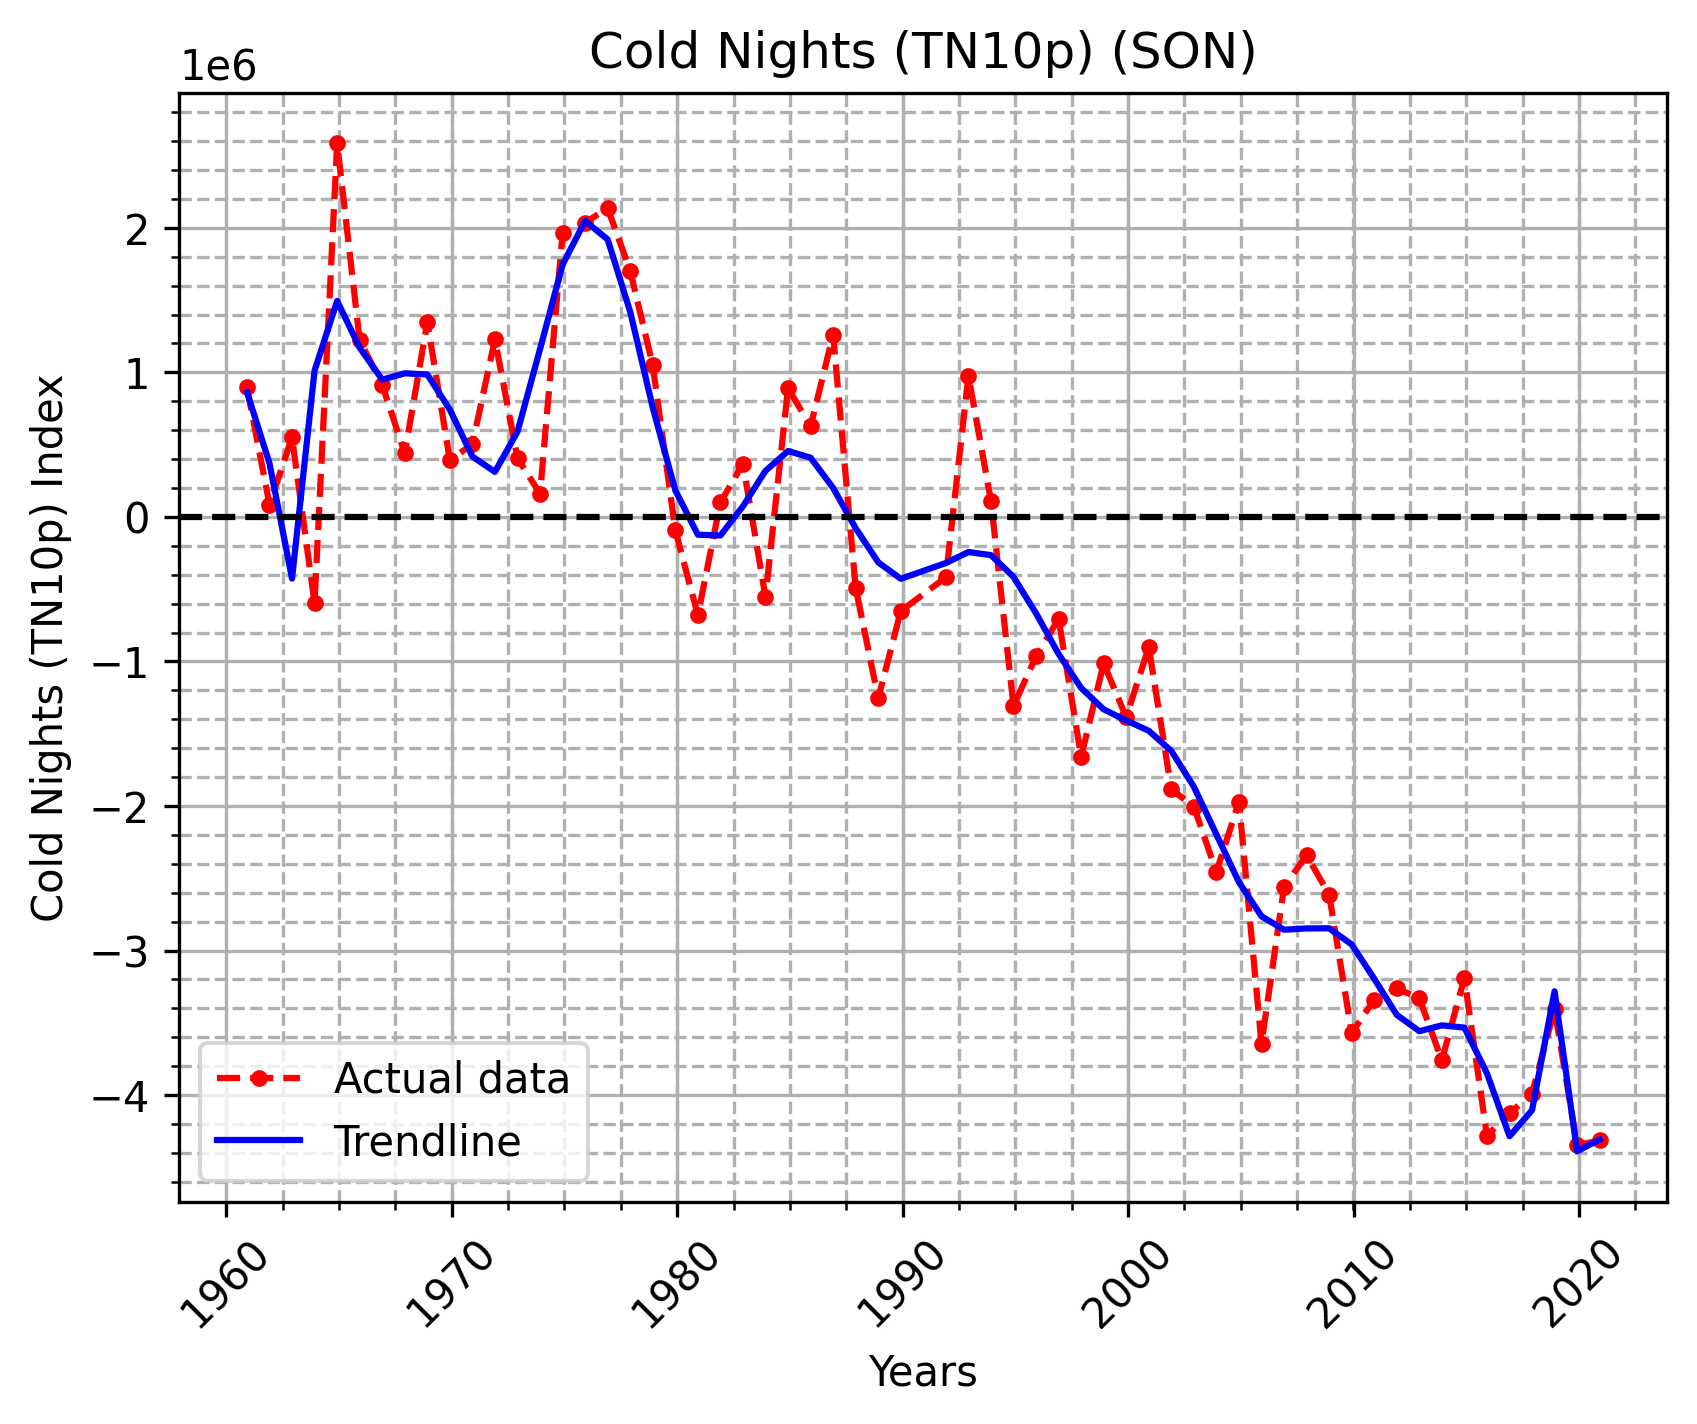
\includegraphics[width=0.75\textwidth]{//home/shiv/Documents/GitHub/EES405/clim_indices/final_plots/cold_nights_son_timeseries.png}
    \caption{Cold Nights (TN10p) (SON) temporal Plot}
    \label{fig:tn10p_son_temporal}
\end{figure}

$ y = -3.42\times10^{3}x^{21}+7.44\times10^{-5}x^{20}-1.88\times10^{-6}x^{19}+3.31\times10^{-10}x^{18}+1.08\times10^{-12}x^{17}-3.97\times10^{-16}x^{16}-1.62\times10^{-19}x^{15}+1.05\times10^{-22}x^{14}-5.80\times10^{-27}x^{13}-8.00\times10^{-30}x^{12}+2.29\times10^{-33}x^{11}-1.20\times10^{-37}x^{10}-6.72\times10^{-41}x^{9}+1.99\times10^{-44}x^{8}-2.95\times10^{-48}x^{7}+2.85\times10^{-52}x^{6}-1.92\times10^{-56}x^{5}+9.12\times10^{-61}x^{4}-3.03\times10^{-65}x^{3}+6.69\times10^{-70}x^{2}-8.87\times10^{-75}x+5.34\times10^{-80}$

The decrease in the frequency of cold nights is consistent with the overall warming of the planet due to climate change as seen in the above spatial plot.\\
Overall, the decrease in the frequency of cold nights is a consistent and expected result of the overall warming of the planet due to climate change.

\section{Seasonal occurance of Warm Nights (TN90p)}
\newpage
\subsection{Spatial plot for warm nights (TN90p) for DJF season}
\begin{figure}[htb]
    \centering
    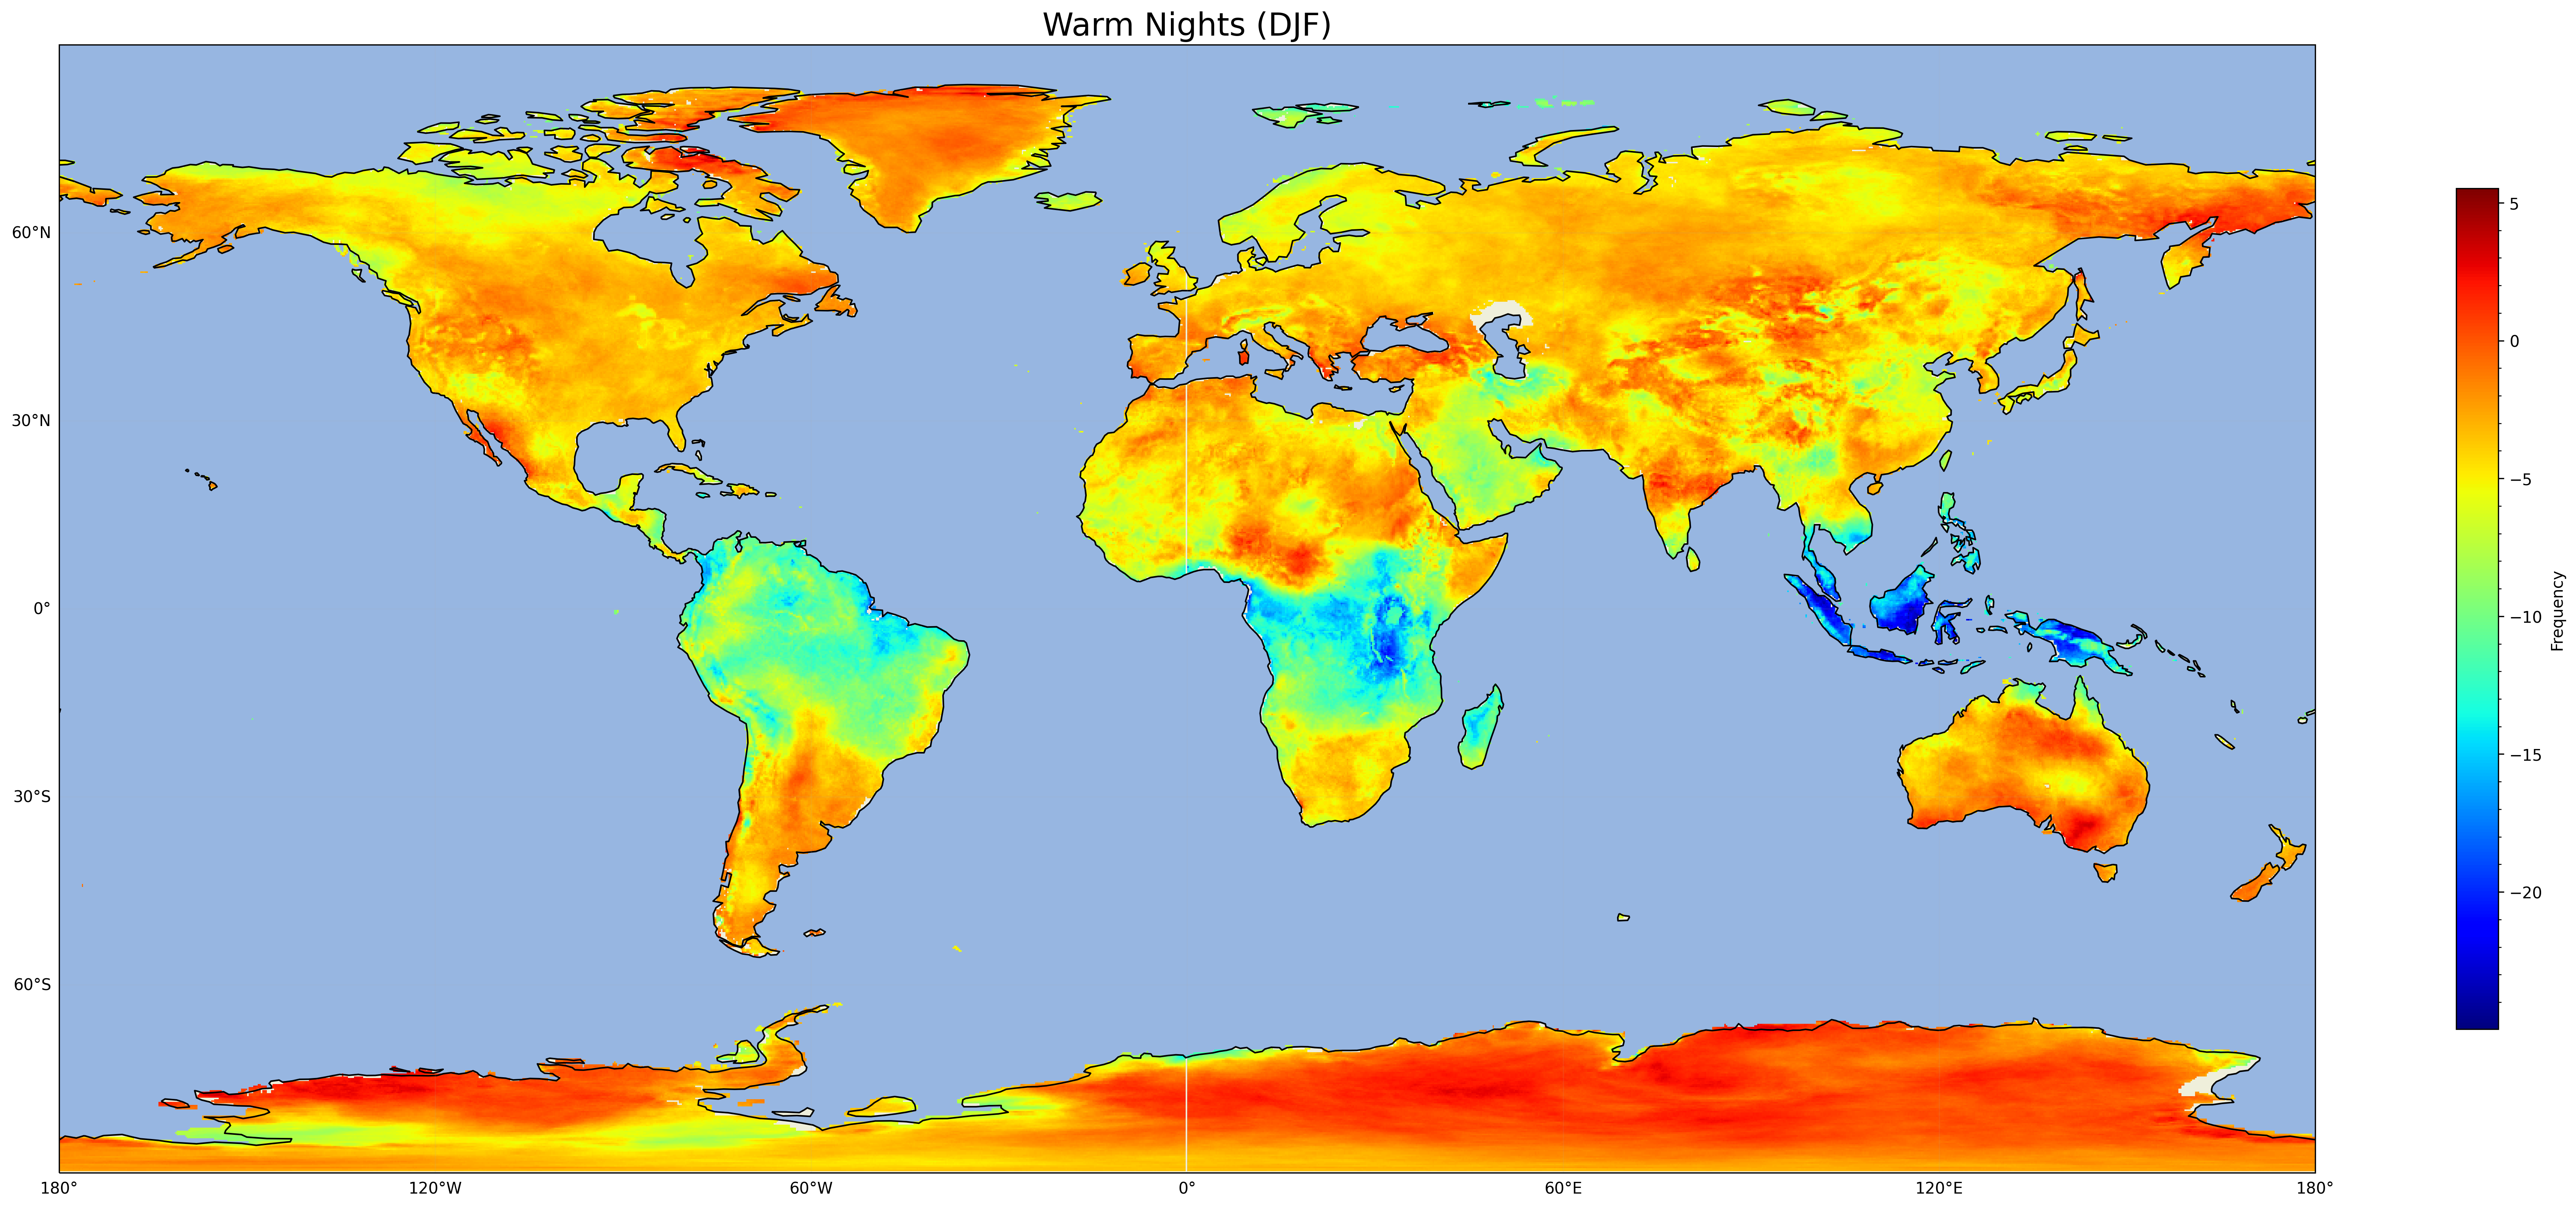
\includegraphics[width=0.80\textwidth]{/home/shiv/Documents/GitHub/EES405/clim_indices/final_plots/tn90p-djf.png}
    \caption{Warm Nights DJF Spatial Plot}
    \label{fig:tn90p_djf_spatial}
\end{figure}

\subsection{Temporal Plot for 'Seasonal occurance of warm nights (TN90p) (DJF)'}
In the above time series plot of cold night anomalies for (DJF) months calculated from the \textbf{TN10p} climate index, we have added a non-linear trendline with polynomial fit of degree 21 (as used in the paper by )given by the following equation.
\begin{figure}[htb]
    \centering
    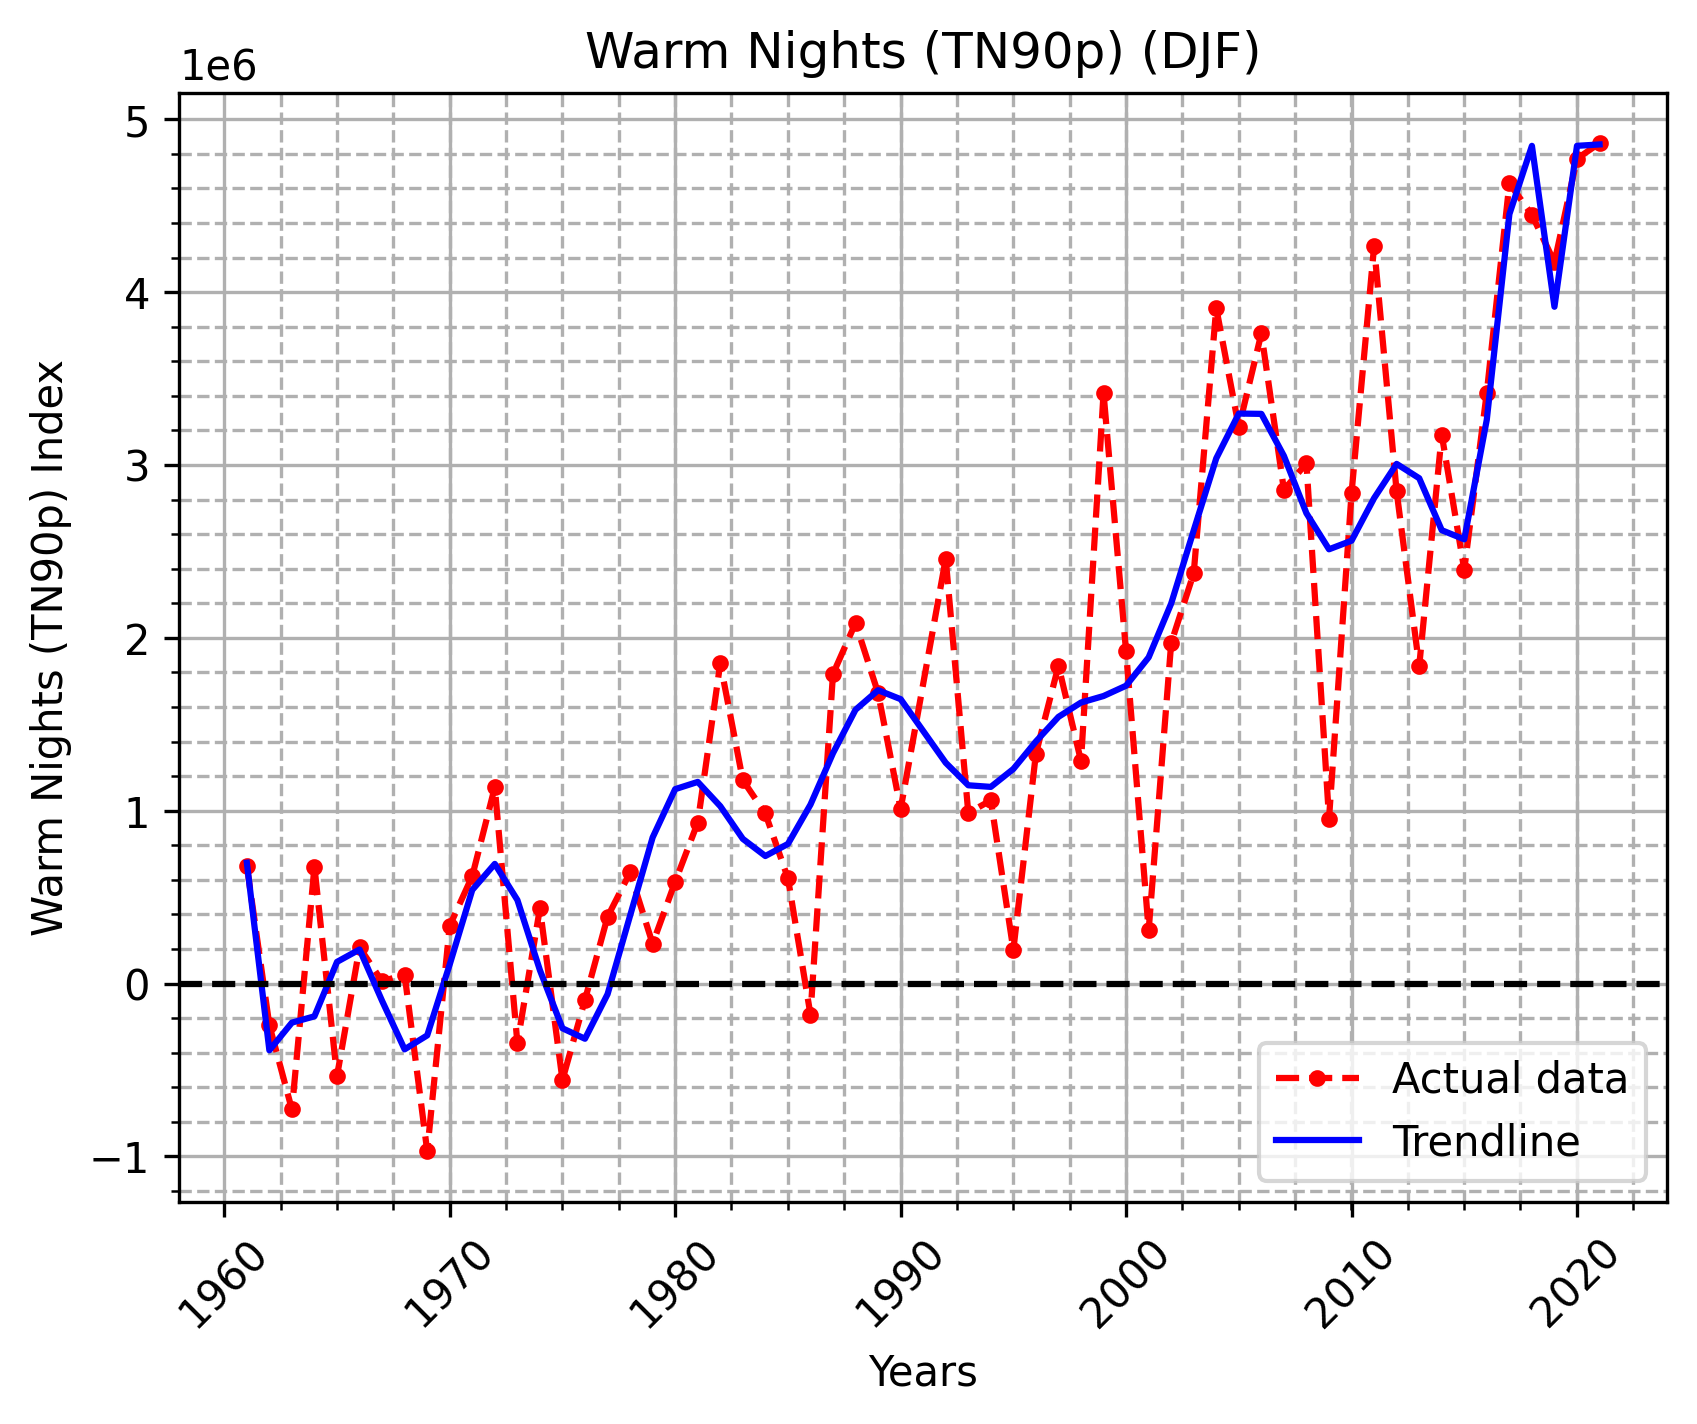
\includegraphics[width=0.75\textwidth]{//home/shiv/Documents/GitHub/EES405/clim_indices/final_plots/warm_nights_djf_timeseries.png}
    \caption{Warm Nights (TN90p) (DJF) temporal Plot}
    \label{fig:tn90p_djf_temporal}
\end{figure}

$ y = -3.42\times10^{3}x^{21}+7.44\times10^{-5}x^{20}-1.88\times10^{-6}x^{19}+3.31\times10^{-10}x^{18}+1.08\times10^{-12}x^{17}-3.97\times10^{-16}x^{16}-1.62\times10^{-19}x^{15}+1.05\times10^{-22}x^{14}-5.80\times10^{-27}x^{13}-8.00\times10^{-30}x^{12}+2.29\times10^{-33}x^{11}-1.20\times10^{-37}x^{10}-6.72\times10^{-41}x^{9}+1.99\times10^{-44}x^{8}-2.95\times10^{-48}x^{7}+2.85\times10^{-52}x^{6}-1.92\times10^{-56}x^{5}+9.12\times10^{-61}x^{4}-3.03\times10^{-65}x^{3}+6.69\times10^{-70}x^{2}-8.87\times10^{-75}x+5.34\times10^{-80}$

The incease in the frequency of warm nights is consistent with the overall warming of the planet due to climate change as seen in the above spatial plot.\\
Overall, the increase in the frequency of cold nights is a consistent and expected result of the overall warming of the planet due to climate change.

\subsection{Spatial plot for warm nights (TN90p) for MAM season}
\begin{figure}[htb]
    \centering
    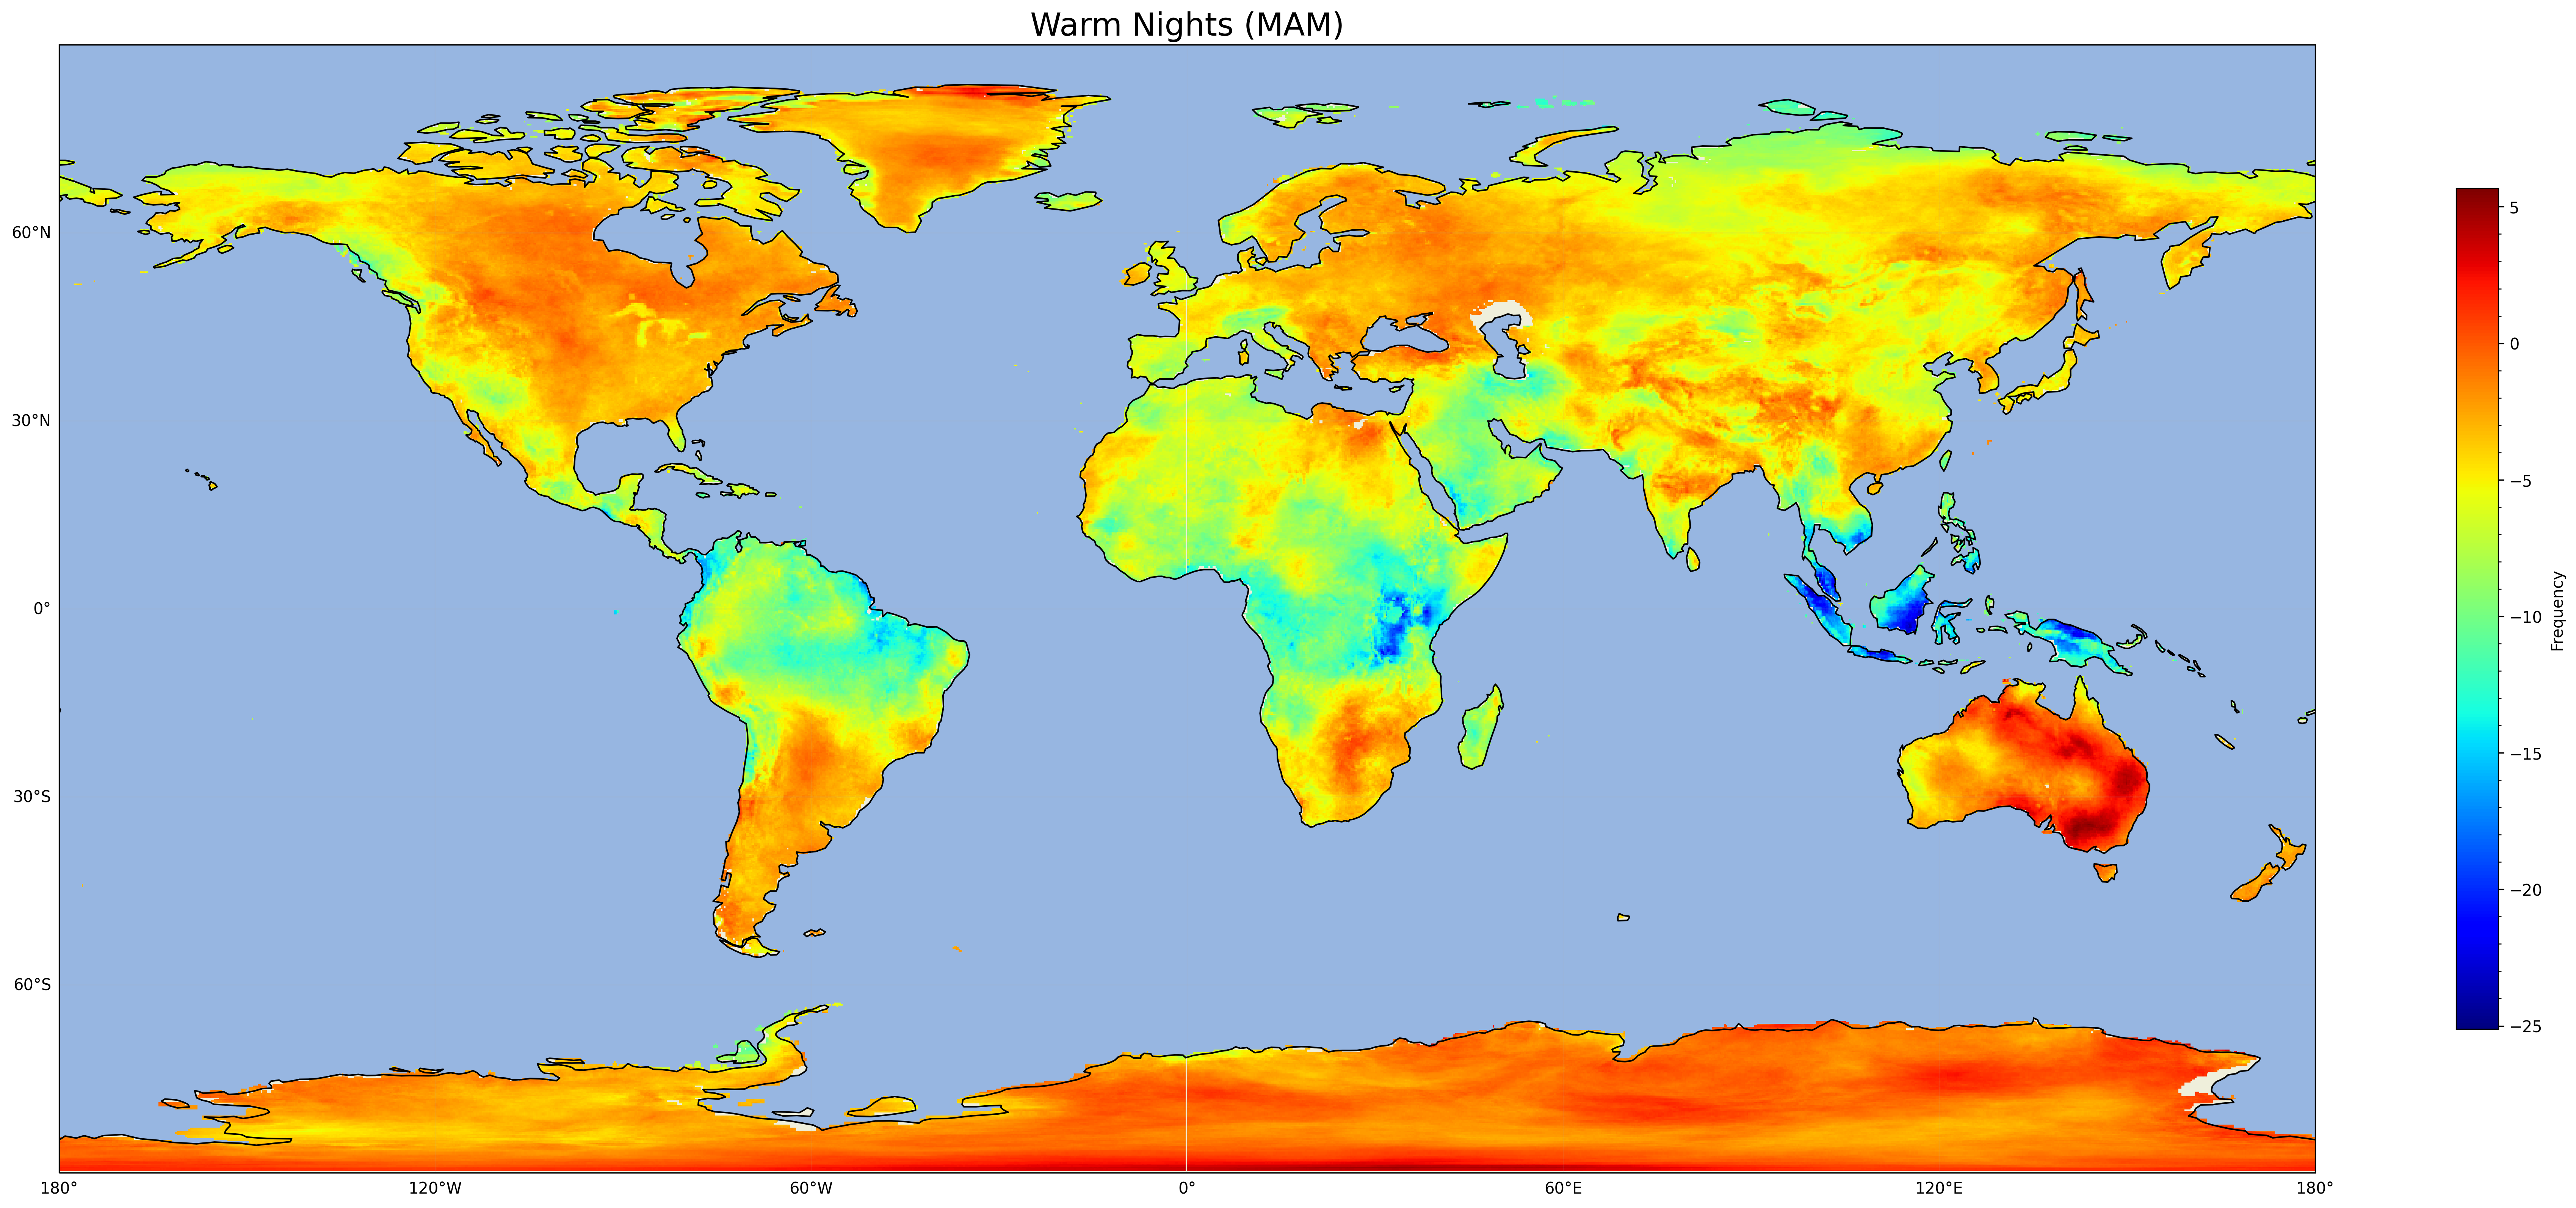
\includegraphics[width=0.80\textwidth]{/home/shiv/Documents/GitHub/EES405/clim_indices/final_plots/tn90p-mam.png}
    \caption{Warm Nights MAM Spatial Plot}
    \label{fig:tn90p_mam_spatial}
\end{figure}

\subsection{Temporal Plot for 'Seasonal occurance of warm nights (TN90p) (MAM)'}
In the above time series plot of cold night anomalies for (MAM) months calculated from the \textbf{TN10p} climate index, we have added a non-linear trendline with polynomial fit of degree 21 (as used in the paper by )given by the following equation. \\
\begin{figure}[htb]
    \centering
    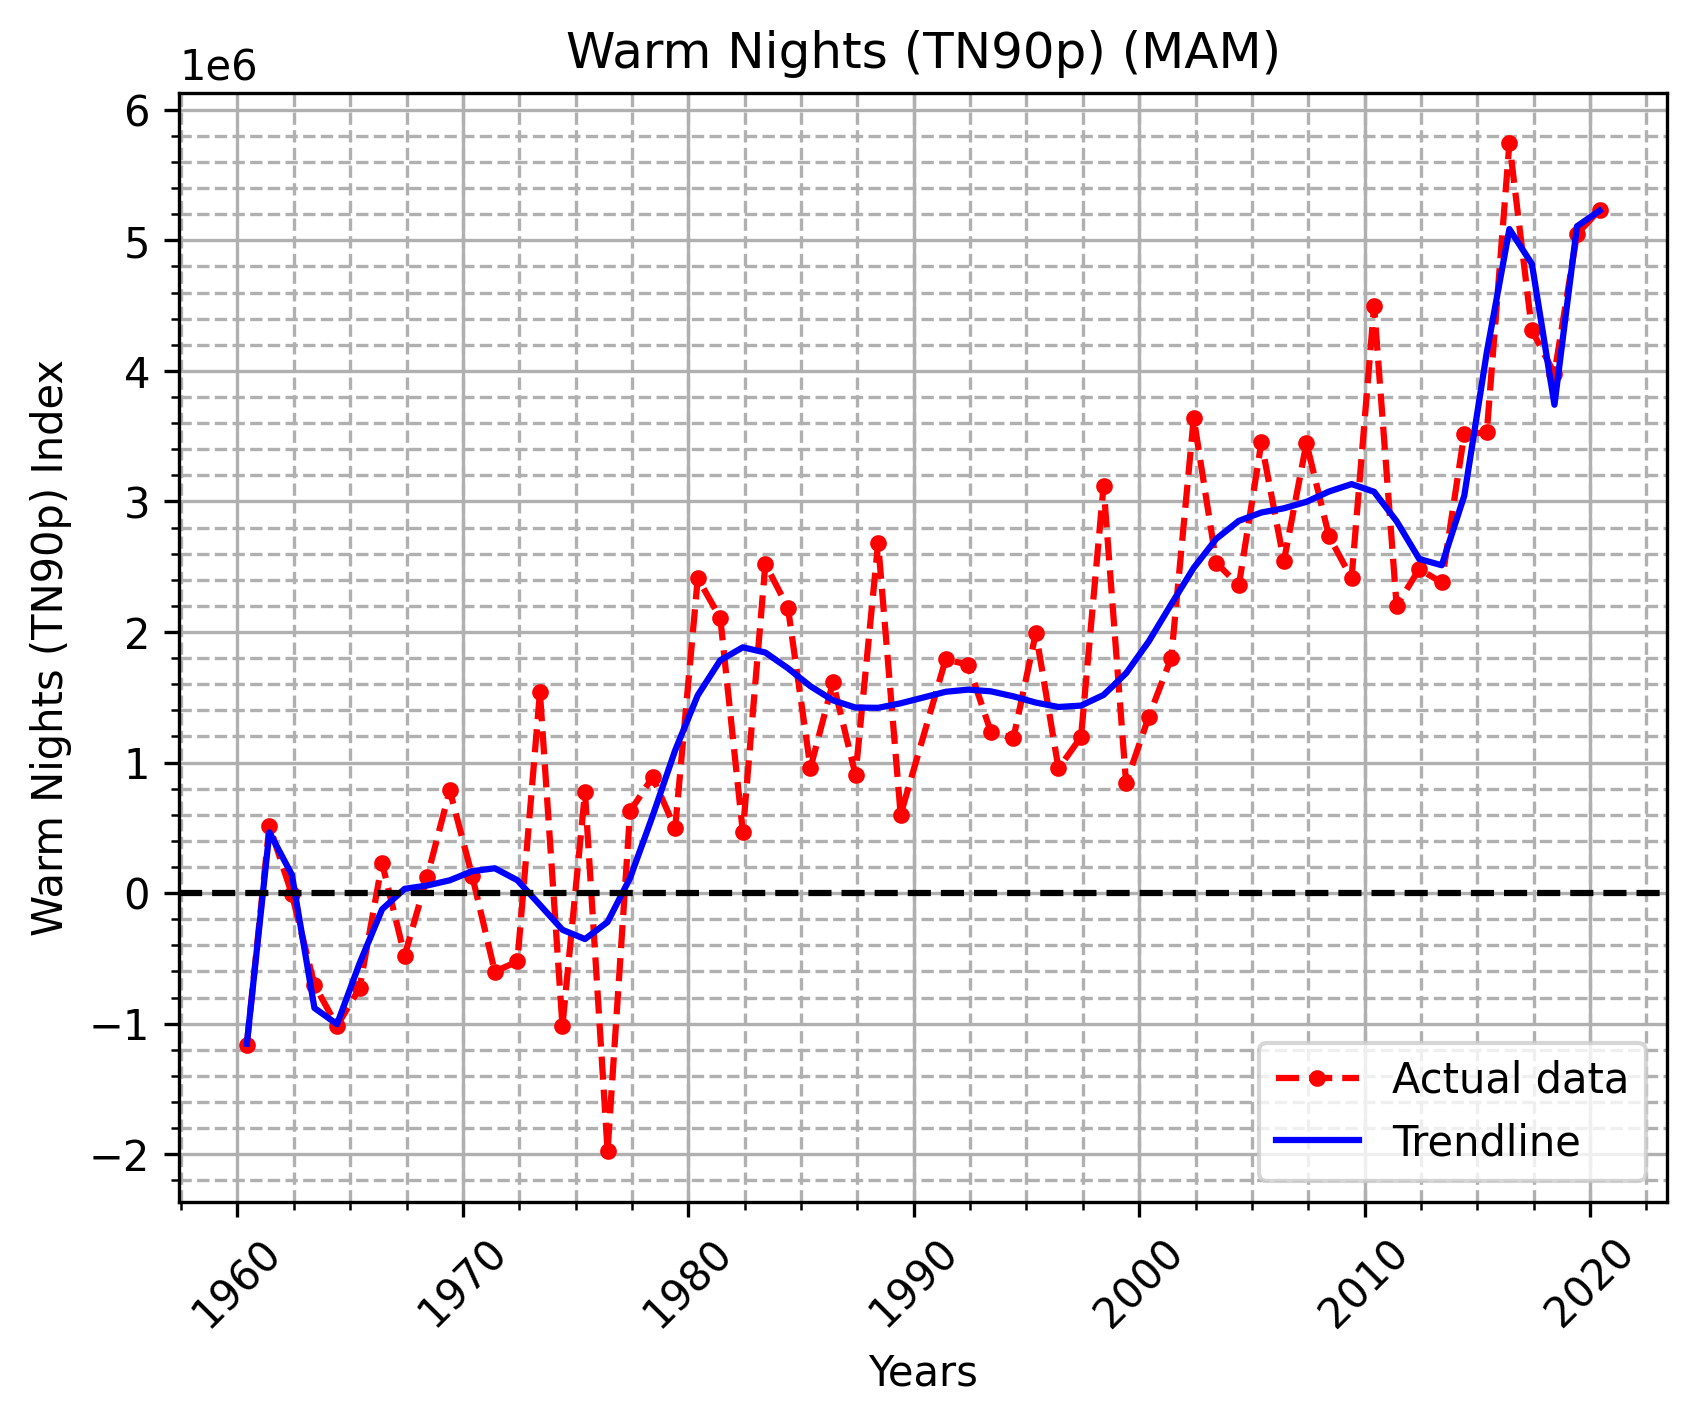
\includegraphics[width=0.75\textwidth]{//home/shiv/Documents/GitHub/EES405/clim_indices/final_plots/warm_nights_mam_timeseries.png}
    \caption{Warm Nights (TN90p) (MAM) temporal Plot}
    \label{fig:tn90p_mam_temporal}
\end{figure}

$ y = -3.42\times10^{3}x^{21}+7.44\times10^{-5}x^{20}-1.88\times10^{-6}x^{19}+3.31\times10^{-10}x^{18}+1.08\times10^{-12}x^{17}-3.97\times10^{-16}x^{16}-1.62\times10^{-19}x^{15}+1.05\times10^{-22}x^{14}-5.80\times10^{-27}x^{13}-8.00\times10^{-30}x^{12}+2.29\times10^{-33}x^{11}-1.20\times10^{-37}x^{10}-6.72\times10^{-41}x^{9}+1.99\times10^{-44}x^{8}-2.95\times10^{-48}x^{7}+2.85\times10^{-52}x^{6}-1.92\times10^{-56}x^{5}+9.12\times10^{-61}x^{4}-3.03\times10^{-65}x^{3}+6.69\times10^{-70}x^{2}-8.87\times10^{-75}x+5.34\times10^{-80}$

The incease in the frequency of warm nights is consistent with the overall warming of the planet due to climate change as seen in the above spatial plot.\\
Overall, the increase in the frequency of cold nights is a consistent and expected result of the overall warming of the planet due to climate change.


\subsection{Spatial plot for warm nights (TN90p) for JJA season}
\begin{figure}[htb]
    \centering
    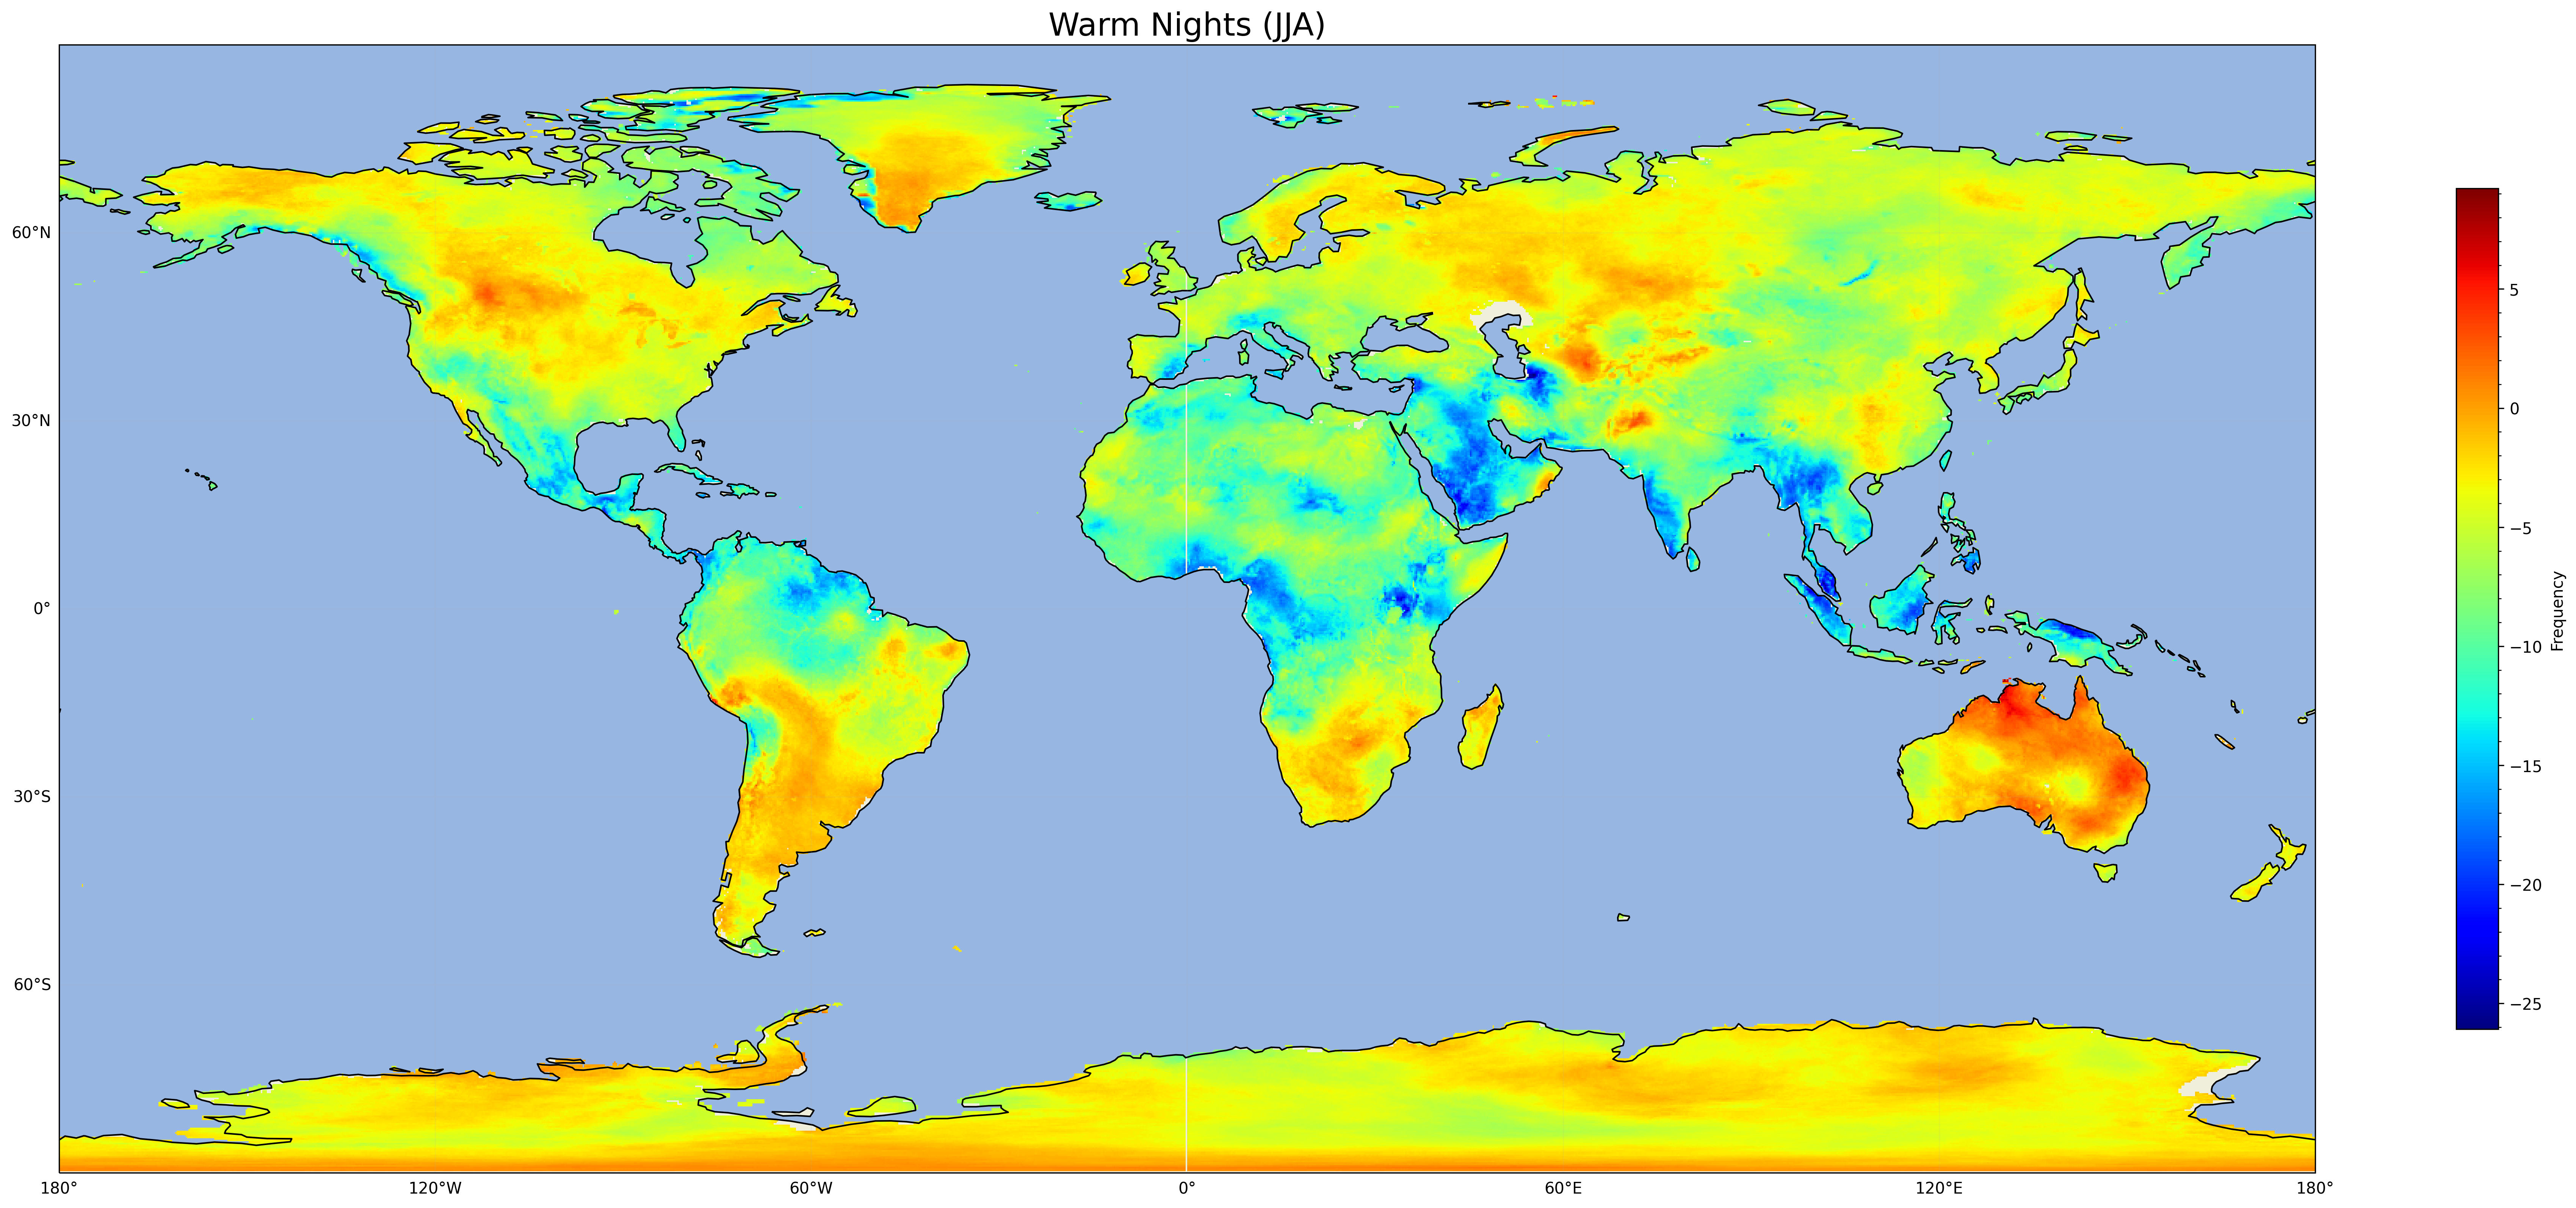
\includegraphics[width=0.80\textwidth]{/home/shiv/Documents/GitHub/EES405/clim_indices/final_plots/tn90p-jja.png}
    \caption{Warm Nights JJA Spatial Plot}
    \label{fig:tn90p_jja_spatial}
\end{figure}

\subsection{Temporal Plot for 'Seasonal occurance of warm nights (TN90p) (JJA)'}
In the above time series plot of cold night anomalies for (JJA) months calculated from the \textbf{TN10p} climate index, we have added a non-linear trendline with polynomial fit of degree 21 (as used in the paper by )given by the following equation. \\
\begin{figure}[htb]
    \centering
    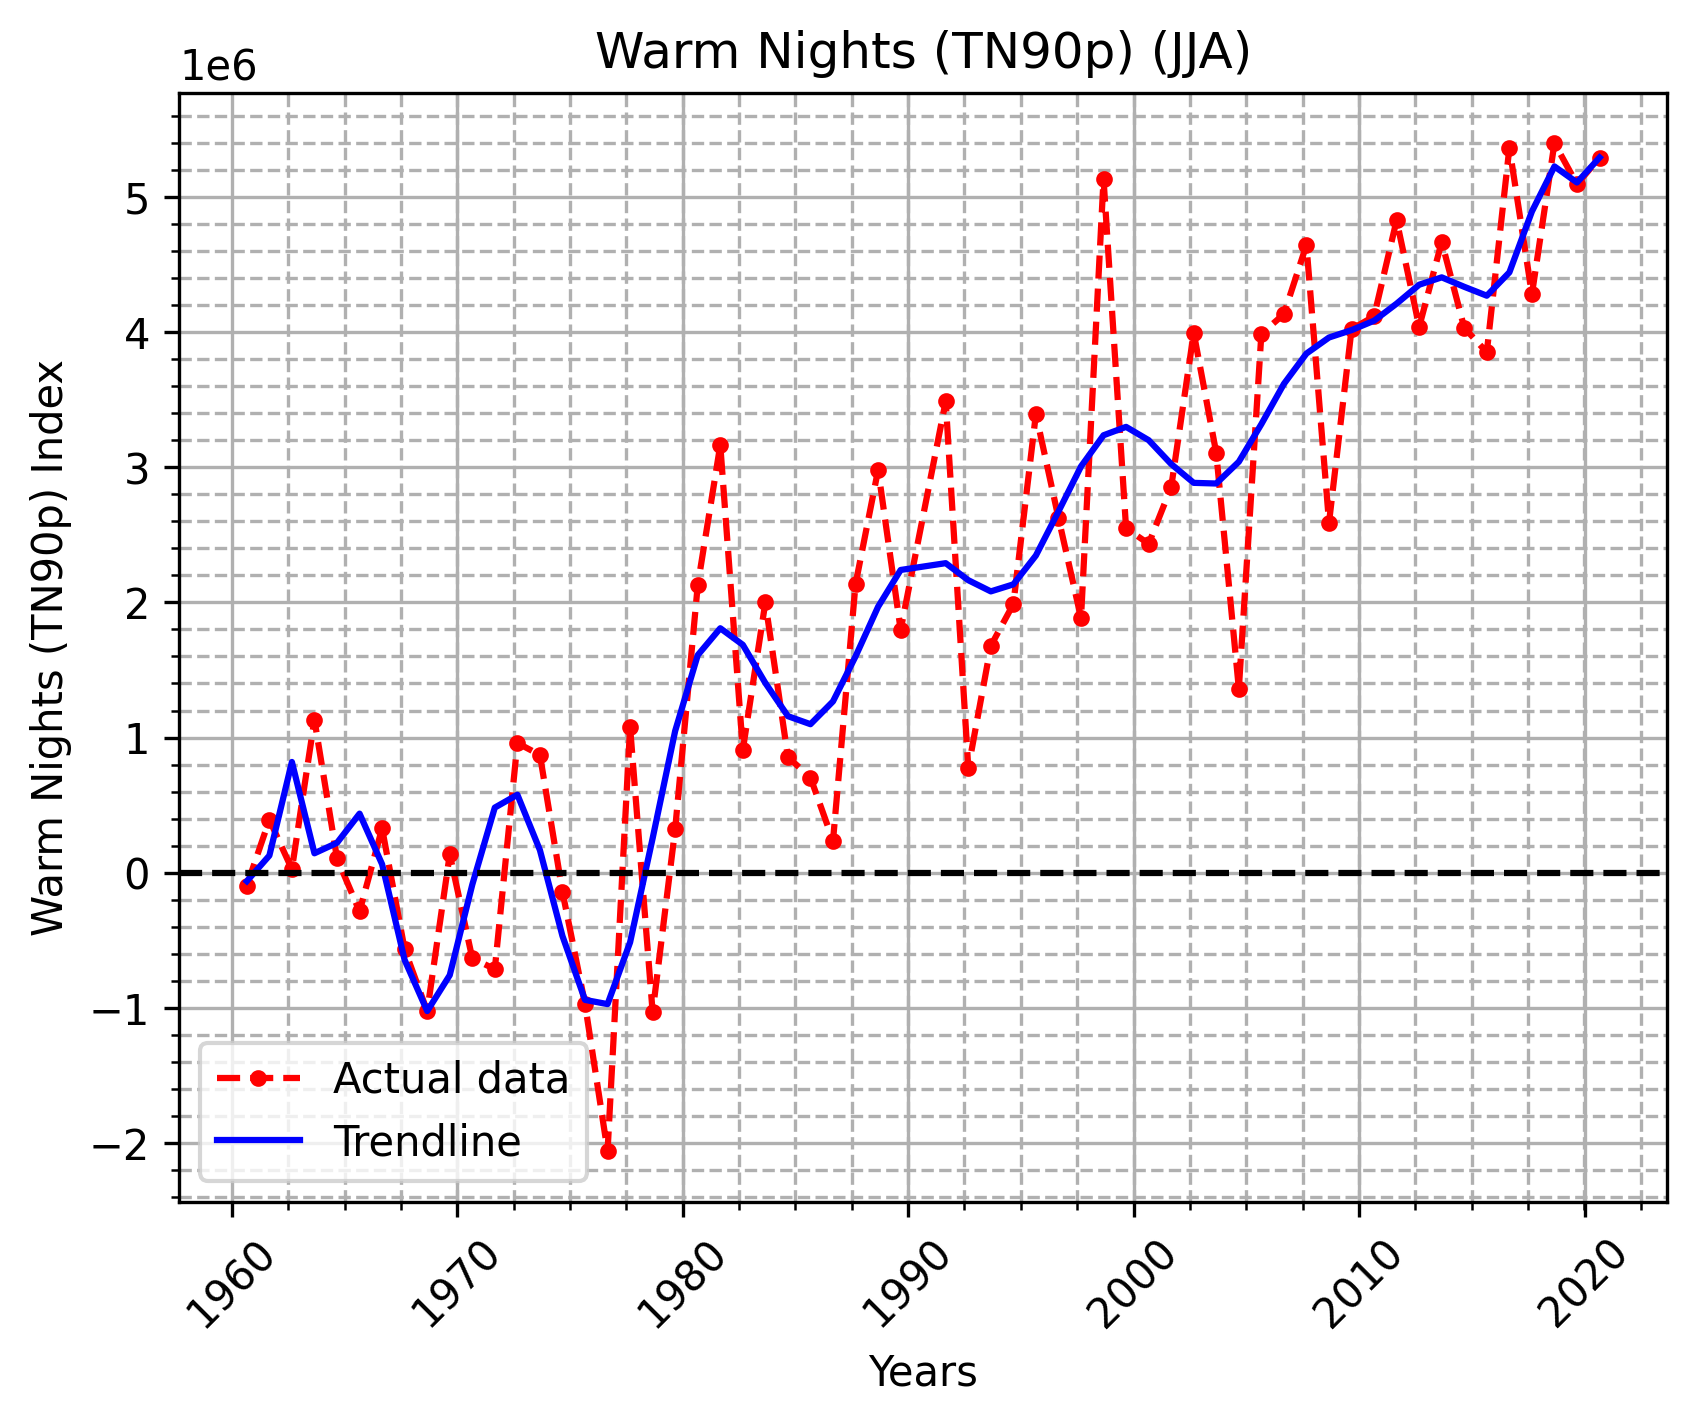
\includegraphics[width=0.75\textwidth]{//home/shiv/Documents/GitHub/EES405/clim_indices/final_plots/warm_nights_jja_timeseries.png}
    \caption{Warm Nights (TN90p) (MAM) temporal Plot}
    \label{fig:tn90p_jja_temporal}
\end{figure}

$ y = -3.42\times10^{3}x^{21}+7.44\times10^{-5}x^{20}-1.88\times10^{-6}x^{19}+3.31\times10^{-10}x^{18}+1.08\times10^{-12}x^{17}-3.97\times10^{-16}x^{16}-1.62\times10^{-19}x^{15}+1.05\times10^{-22}x^{14}-5.80\times10^{-27}x^{13}-8.00\times10^{-30}x^{12}+2.29\times10^{-33}x^{11}-1.20\times10^{-37}x^{10}-6.72\times10^{-41}x^{9}+1.99\times10^{-44}x^{8}-2.95\times10^{-48}x^{7}+2.85\times10^{-52}x^{6}-1.92\times10^{-56}x^{5}+9.12\times10^{-61}x^{4}-3.03\times10^{-65}x^{3}+6.69\times10^{-70}x^{2}-8.87\times10^{-75}x+5.34\times10^{-80}$

The incease in the frequency of warm nights is consistent with the overall warming of the planet due to climate change as seen in the above spatial plot.\\
Overall, the increase in the frequency of cold nights is a consistent and expected result of the overall warming of the planet due to climate change.

\newpage

\subsection{Spatial plot for warm nights (TN90p) for SON season}
\begin{figure}[htb]
    \centering
    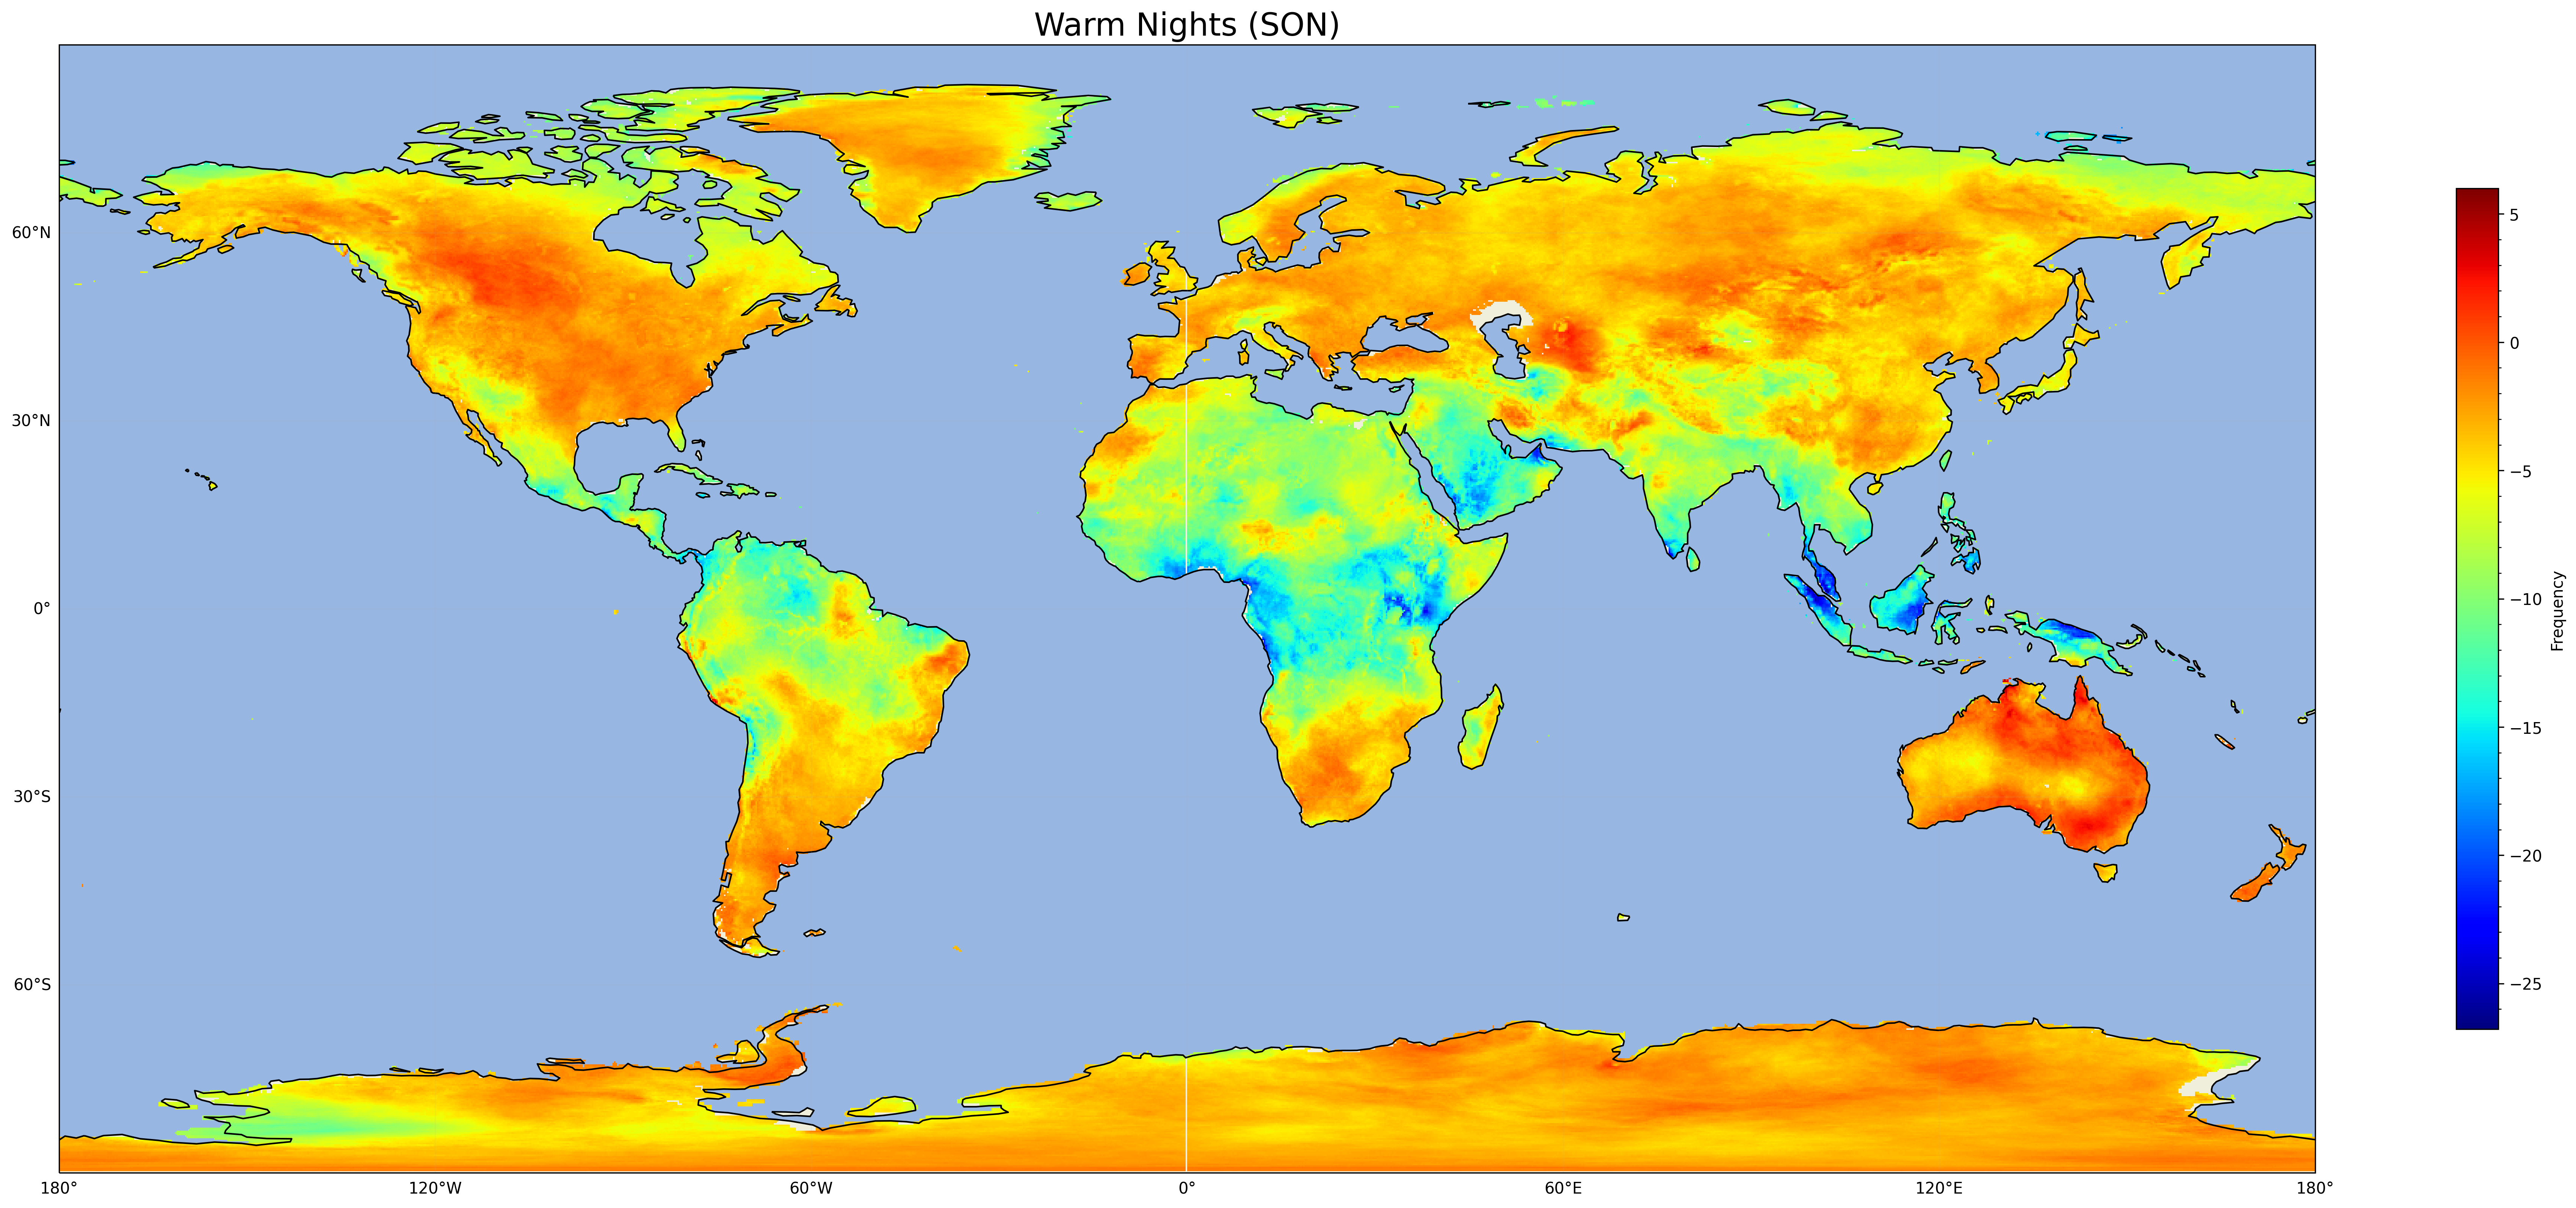
\includegraphics[width=0.80\textwidth]{/home/shiv/Documents/GitHub/EES405/clim_indices/final_plots/tn90p-son.png}
    \caption{Warm Nights SON Spatial Plot}
    \label{fig:tn90p_son_spatial}
\end{figure}

\subsection{Temporal Plot for 'Seasonal occurance of warm nights (TN90p) (SON)'}
In the above time series plot of cold night anomalies for (SON) months calculated from the \textbf{TN10p} climate index, we have added a non-linear trendline with polynomial fit of degree 21 (as used in the paper by )given by the following equation.
\begin{figure}[htb]
    \centering
    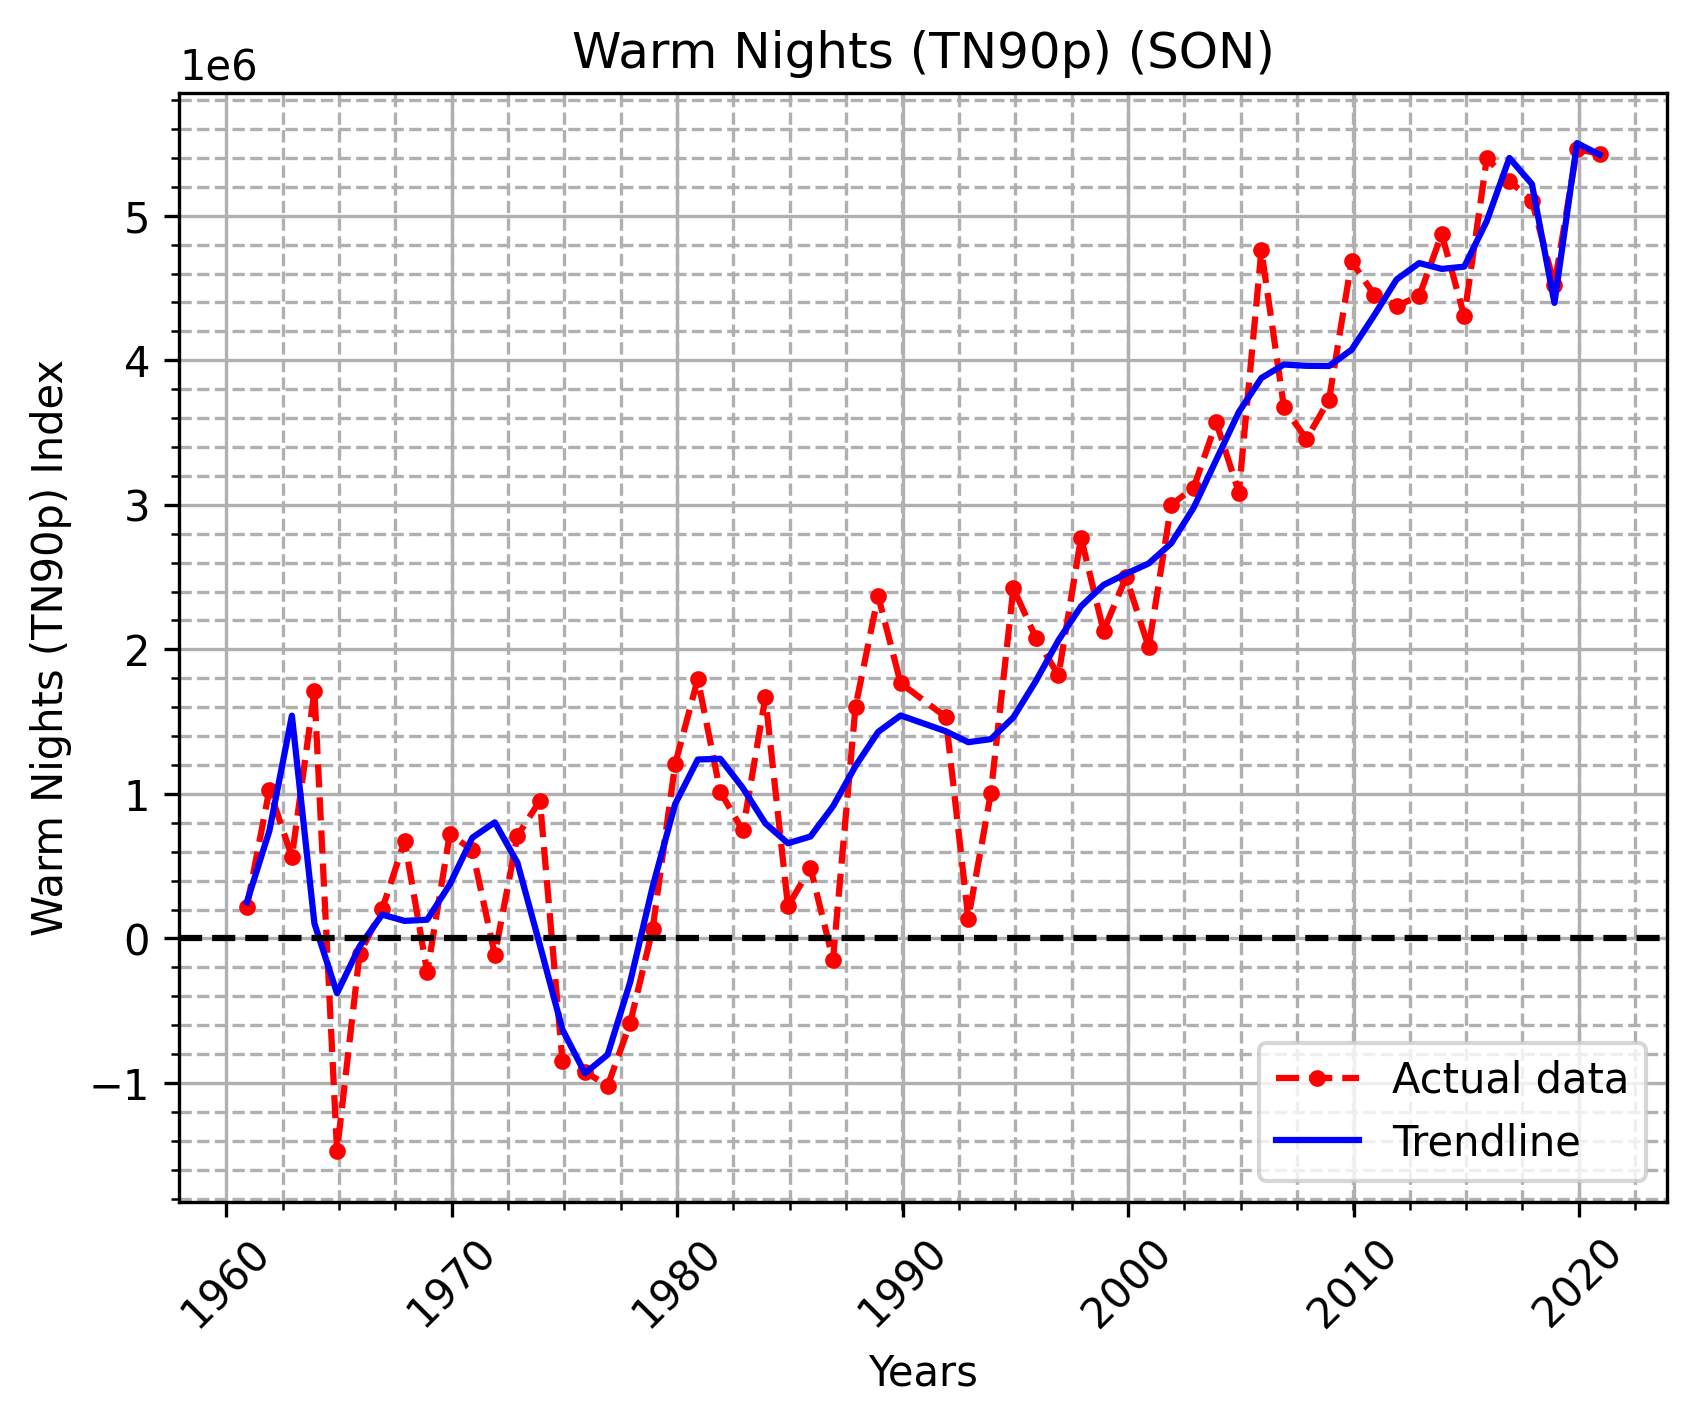
\includegraphics[width=0.75\textwidth]{//home/shiv/Documents/GitHub/EES405/clim_indices/final_plots/warm_nights_son_timeseries.png}
    \caption{Warm Nights (TN90p) (SON) temporal Plot}
    \label{fig:tn90p_son_temporal}
\end{figure}

$ y = -3.42\times10^{3}x^{21}+7.44\times10^{-5}x^{20}-1.88\times10^{-6}x^{19}+3.31\times10^{-10}x^{18}+1.08\times10^{-12}x^{17}-3.97\times10^{-16}x^{16}-1.62\times10^{-19}x^{15}+1.05\times10^{-22}x^{14}-5.80\times10^{-27}x^{13}-8.00\times10^{-30}x^{12}+2.29\times10^{-33}x^{11}-1.20\times10^{-37}x^{10}-6.72\times10^{-41}x^{9}+1.99\times10^{-44}x^{8}-2.95\times10^{-48}x^{7}+2.85\times10^{-52}x^{6}-1.92\times10^{-56}x^{5}+9.12\times10^{-61}x^{4}-3.03\times10^{-65}x^{3}+6.69\times10^{-70}x^{2}-8.87\times10^{-75}x+5.34\times10^{-80}$

The incease in the frequency of warm nights is consistent with the overall warming of the planet due to climate change as seen in the above spatial plot.\\
Overall, the increase in the frequency of cold nights is a consistent and expected result of the overall warming of the planet due to climate change.

\section {Heavy Precipitation days}
% \subsection{Spatial plot for heavy precipitation days (R10mm)}
% \begin{figure}[htb]
%     \centering
%     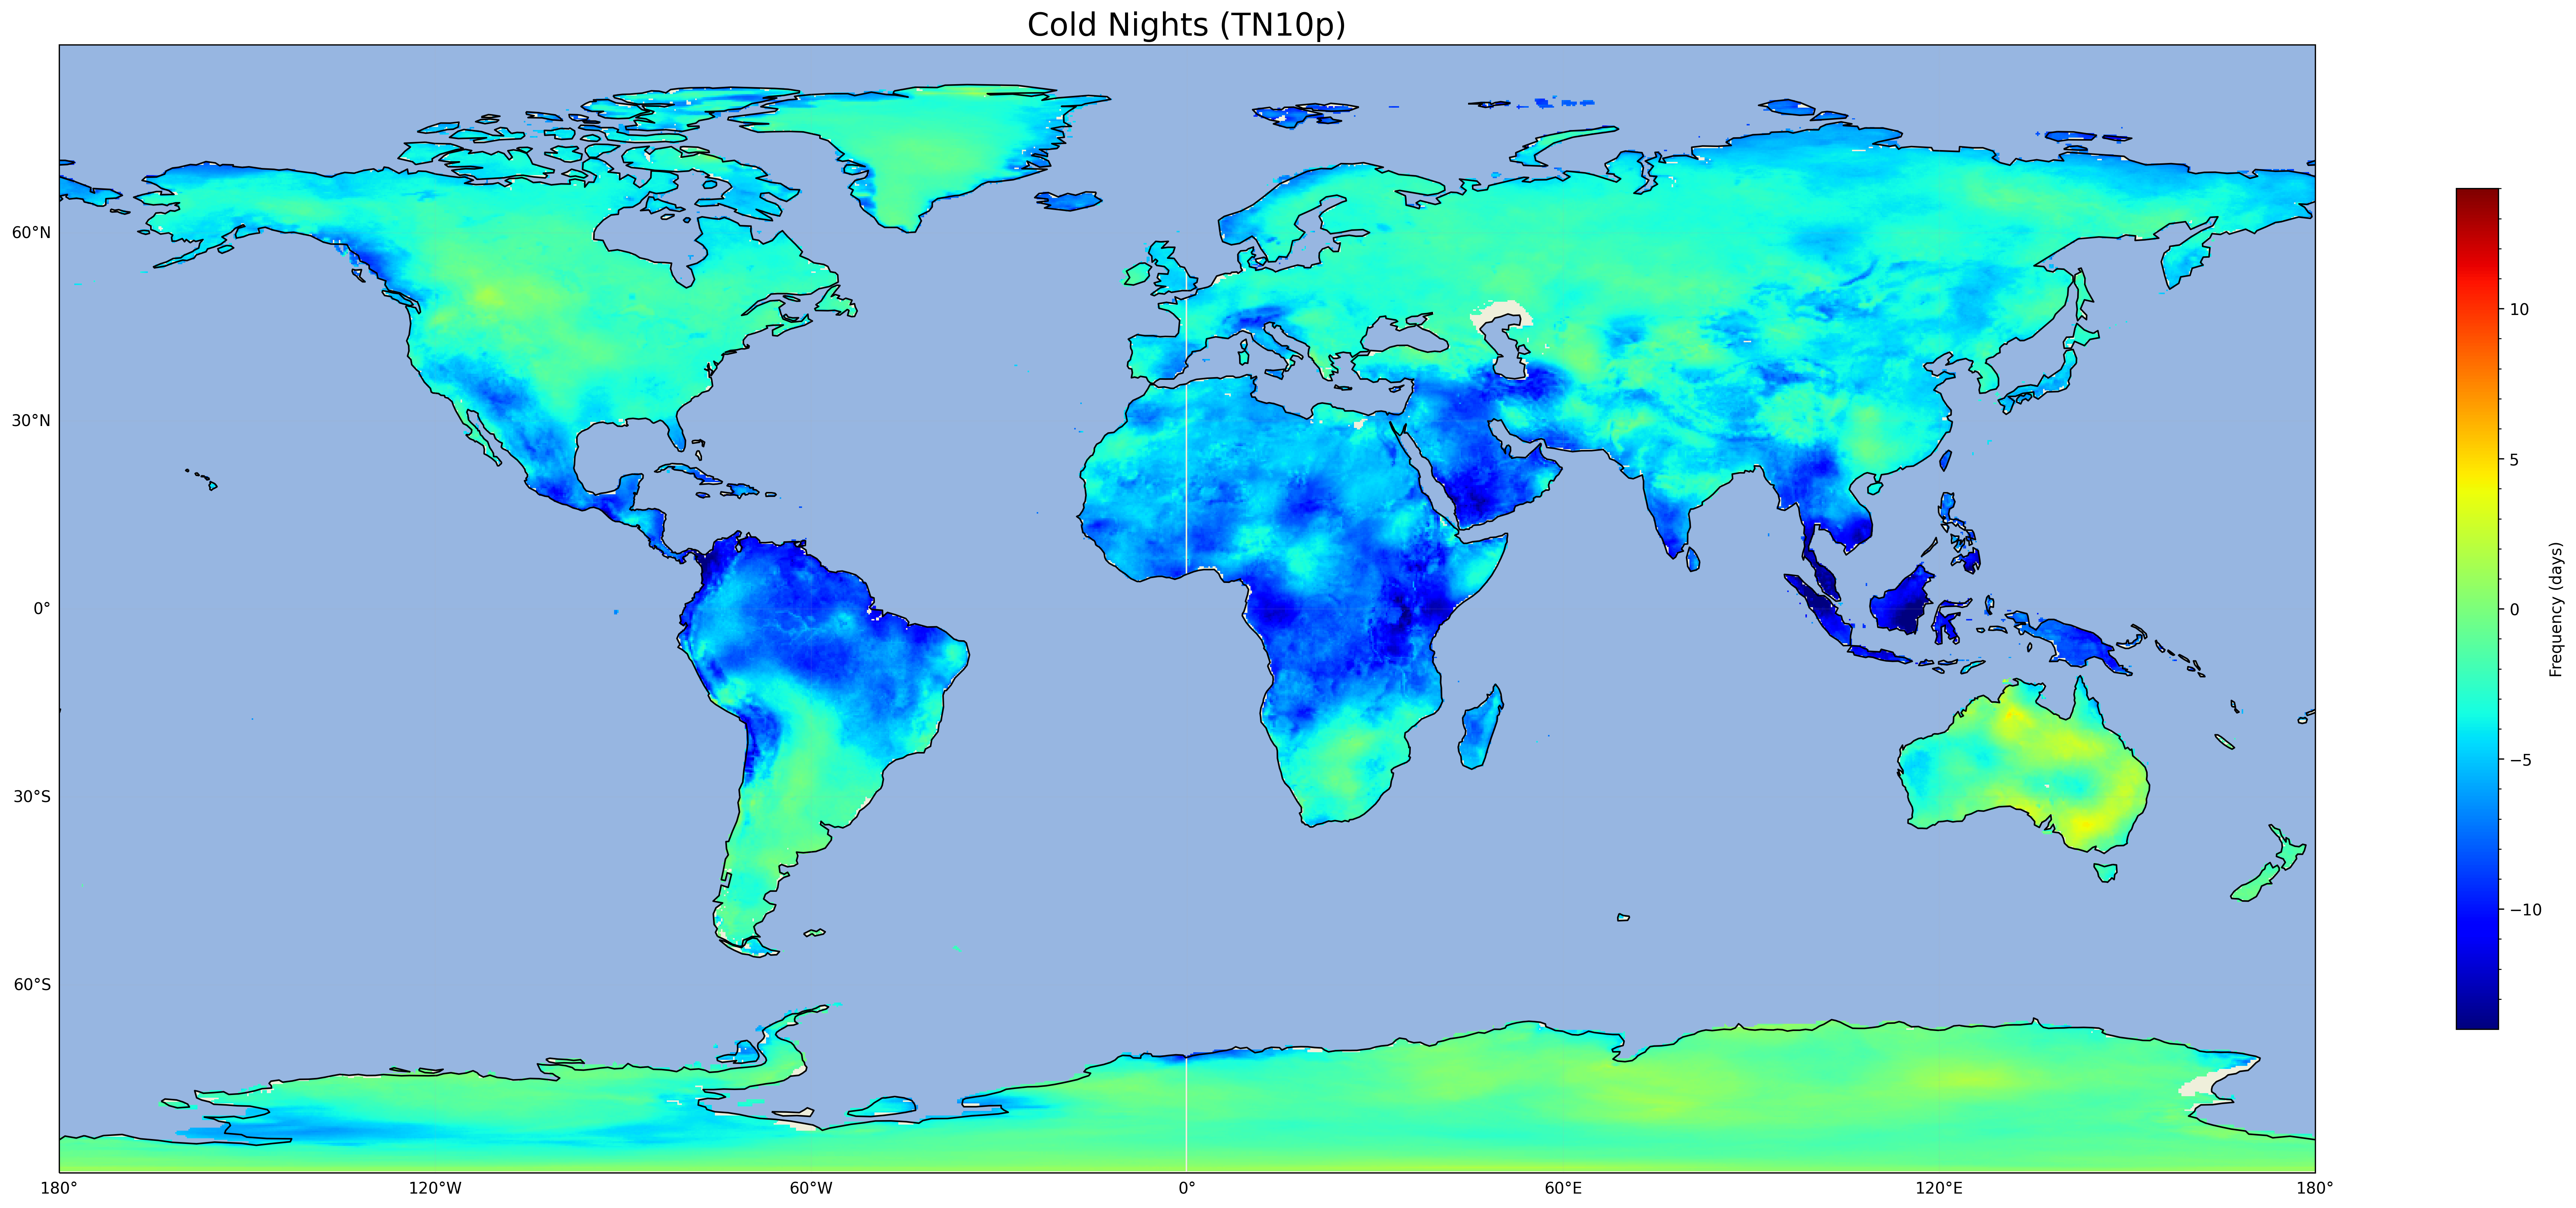
\includegraphics[width=0.80\textwidth]{/home/shiv/Documents/GitHub/EES405/clim_extreme/plots_clim_extreme/cold_nights.png}
%     \caption{Warm days Spatial Plot}
%     \label{fig:r10mm_spatial}
% \end{figure}

\subsection{Temporal Plot for 'Heavy precipitation days (R10mm)'}
In the above time series plot of heavy precipitation days anomalies calculated from the \textbf{R10mm} climate index, we have added a non-linear trendline with polynomial fit of degree 21 (as used in the paper by )given by the following equation. \\
\begin{figure}[htb]
    \centering
    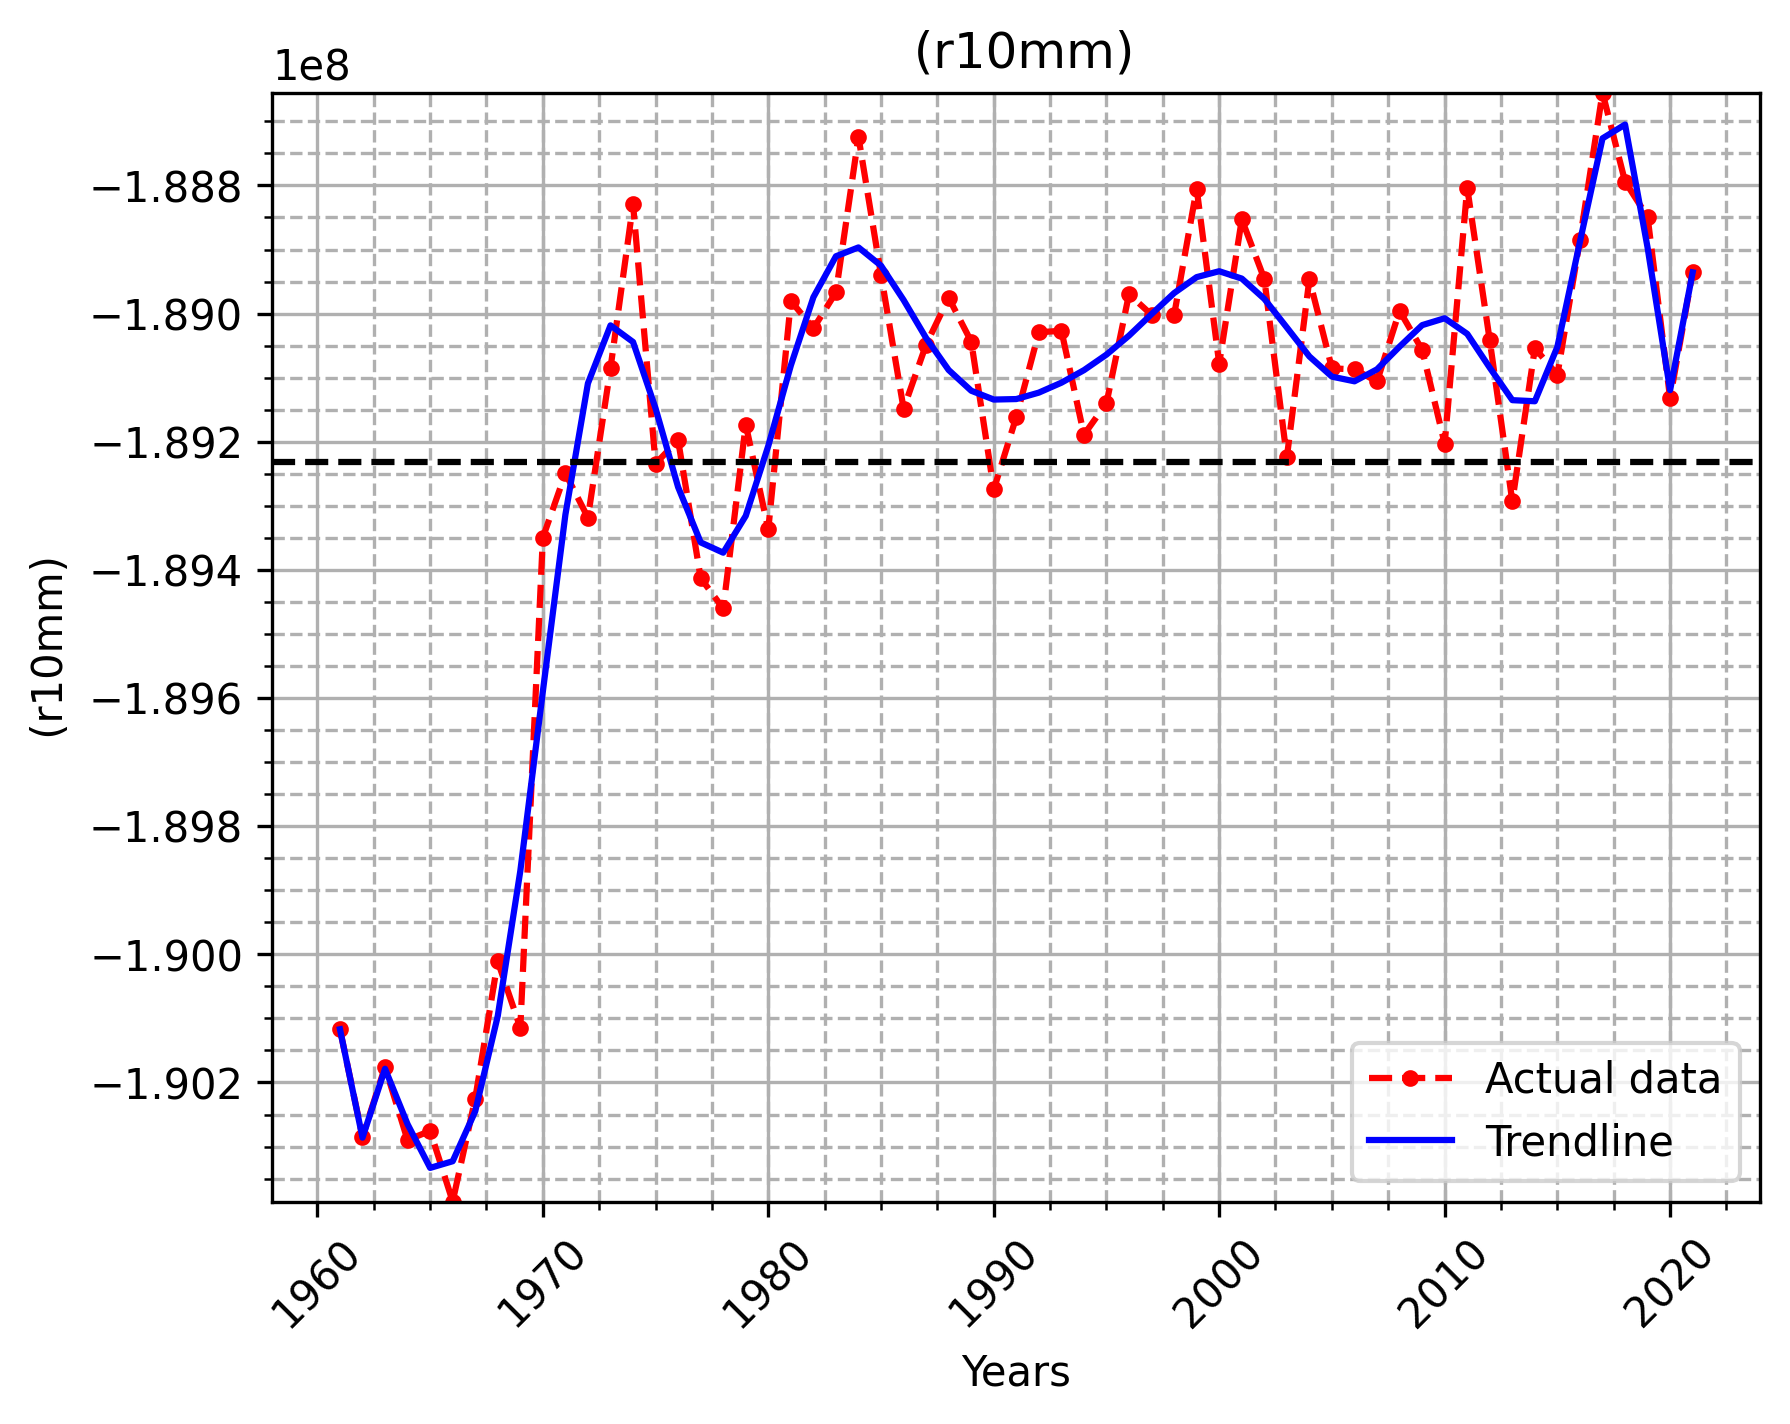
\includegraphics[width=0.75\textwidth]{//home/shiv/Documents/GitHub/EES405/clim_indices/final_plots/heavy_prec.png}
    \caption{Heavy precipitation days (R10mm) temporal Plot}
    \label{fig:r10mm_temporal}
\end{figure}

$ y = -3.42\times10^{3}x^{21}+7.44\times10^{-5}x^{20}-1.88\times10^{-6}x^{19}+3.31\times10^{-10}x^{18}+1.08\times10^{-12}x^{17}-3.97\times10^{-16}x^{16}-1.62\times10^{-19}x^{15}+1.05\times10^{-22}x^{14}-5.80\times10^{-27}x^{13}-8.00\times10^{-30}x^{12}+2.29\times10^{-33}x^{11}-1.20\times10^{-37}x^{10}-6.72\times10^{-41}x^{9}+1.99\times10^{-44}x^{8}-2.95\times10^{-48}x^{7}+2.85\times10^{-52}x^{6}-1.92\times10^{-56}x^{5}+9.12\times10^{-61}x^{4}-3.03\times10^{-65}x^{3}+6.69\times10^{-70}x^{2}-8.87\times10^{-75}x+5.34\times10^{-80}$

The incease in the frequency of heavy precipitation days is consistent with the overall warming of the planet due to climate change as seen in the above spatial plot.\\
Overall, the increase in the frequency of cold nights is a consistent and expected result of the overall warming of the planet due to climate change.
\section{Very wet days}
\subsection{Spatial plot for very wet days (R95p)}
\begin{figure}[htb]
    \centering
    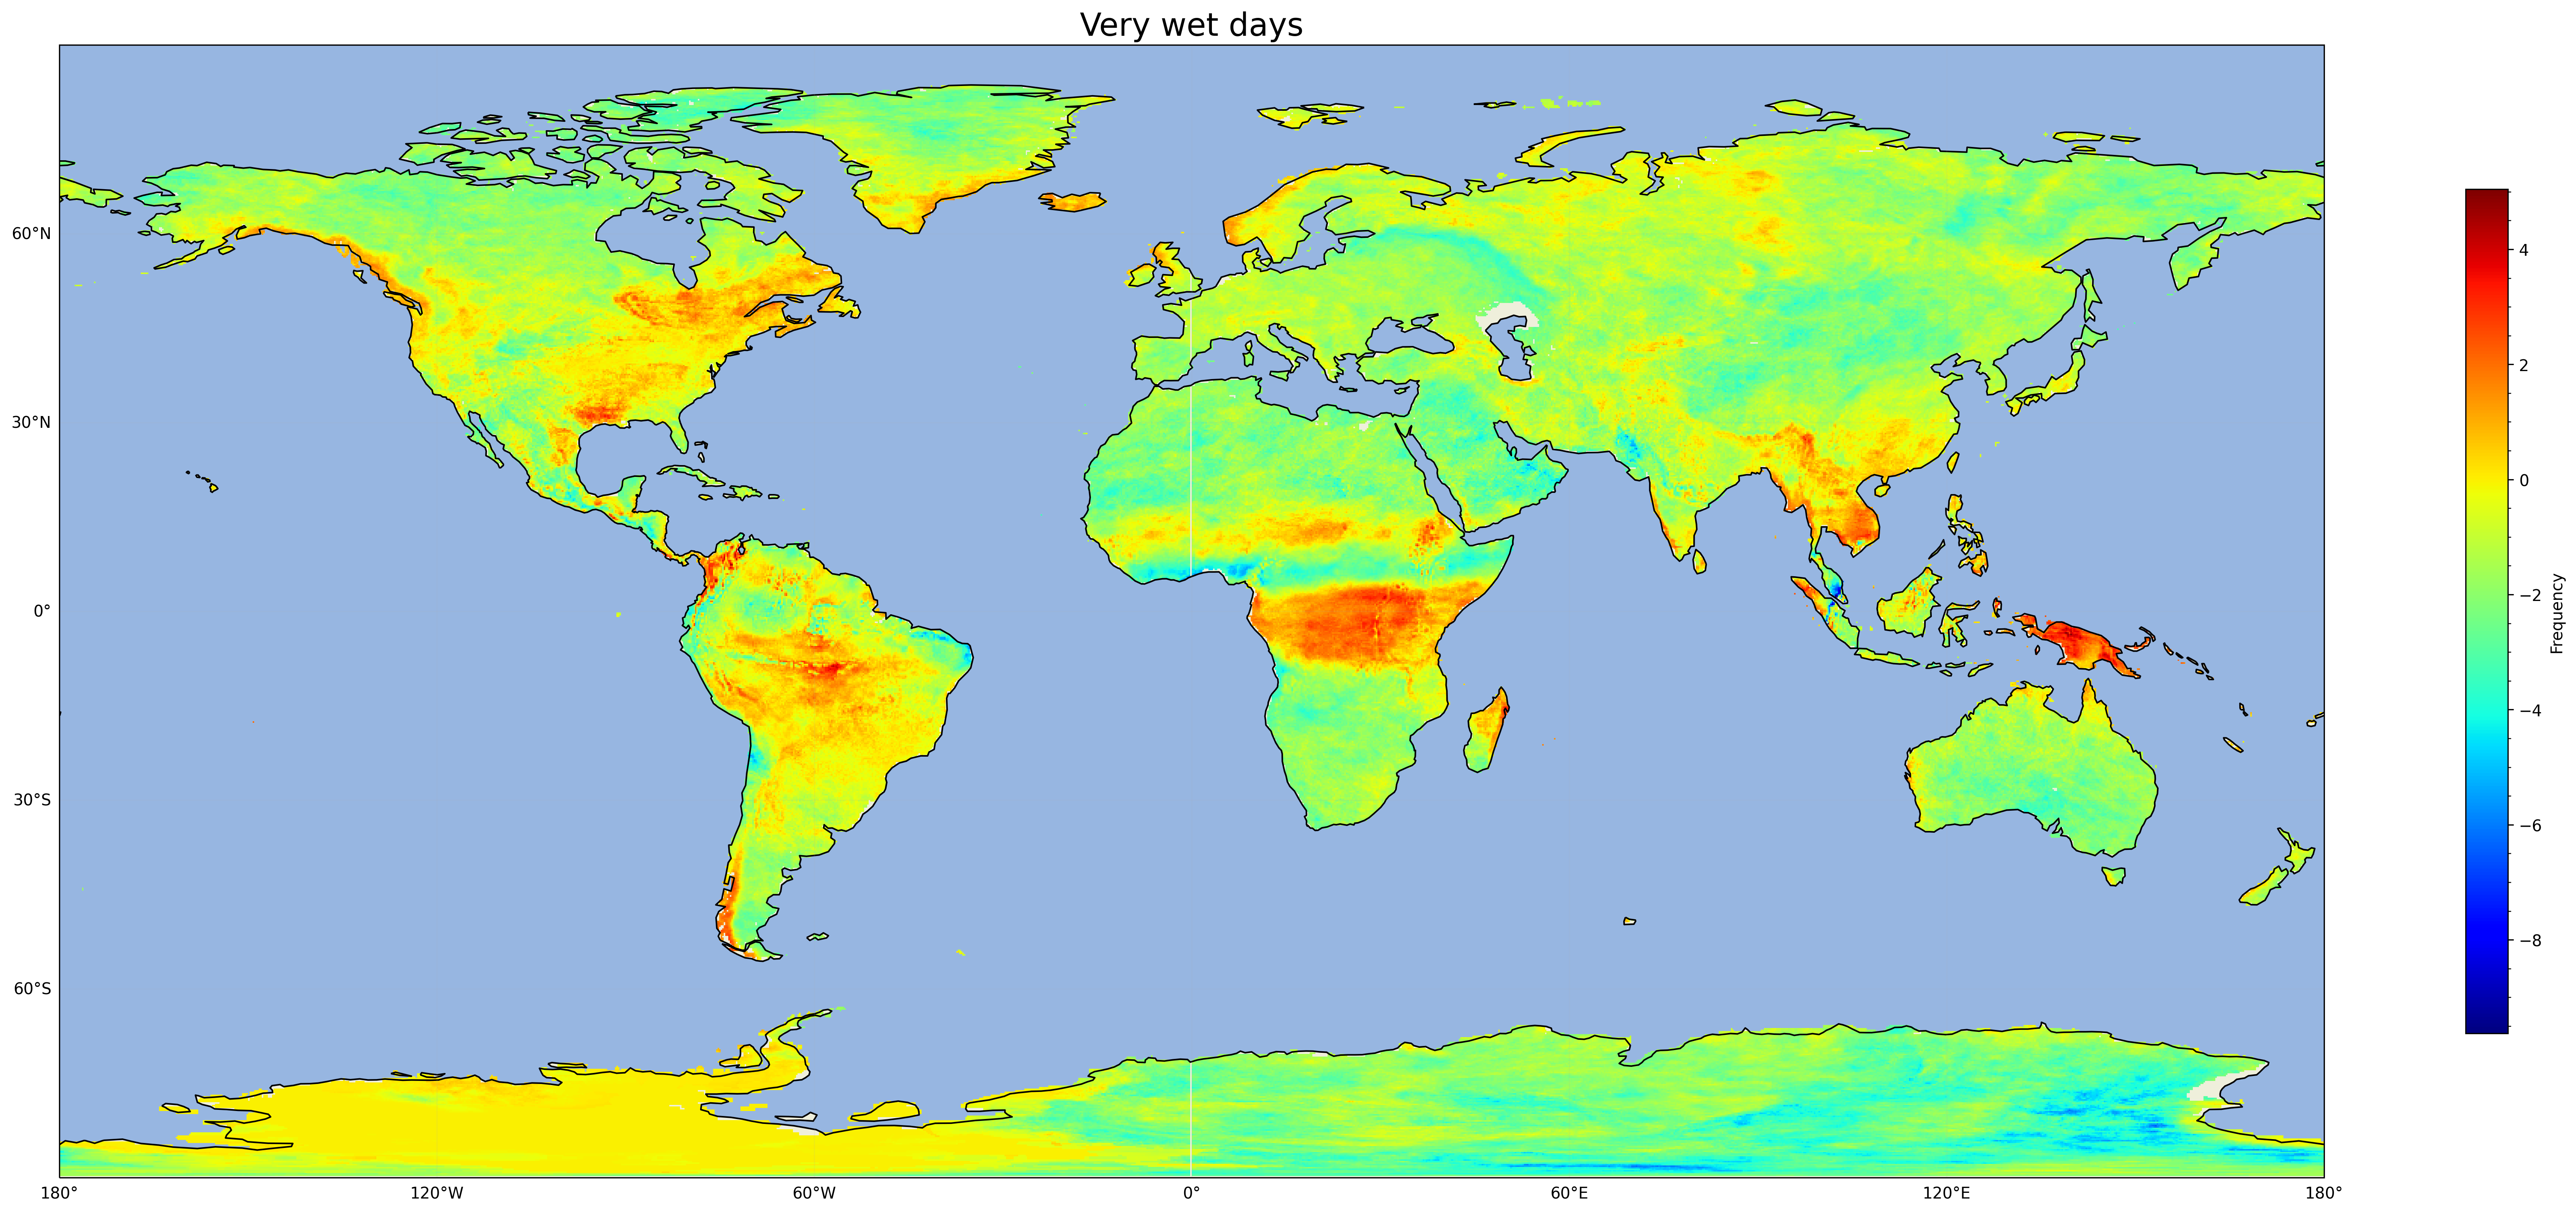
\includegraphics[width=0.80\textwidth]{/home/shiv/Documents/GitHub/EES405/clim_indices/final_plots/very-wet-days.png}
    \caption{Very wet days Spatial Plot}
    \label{fig:r95p_spatial}
\end{figure}

\subsection{Temporal Plot for 'Very wet days (R95p)'}
In the above time series plot of very wet days anomalies calculated from the \textbf{R95p} climate index, we have added a non-linear trendline with polynomial fit of degree 21 (as used in the paper by )given by the following equation. \\
\begin{figure}[htb]
    \centering
    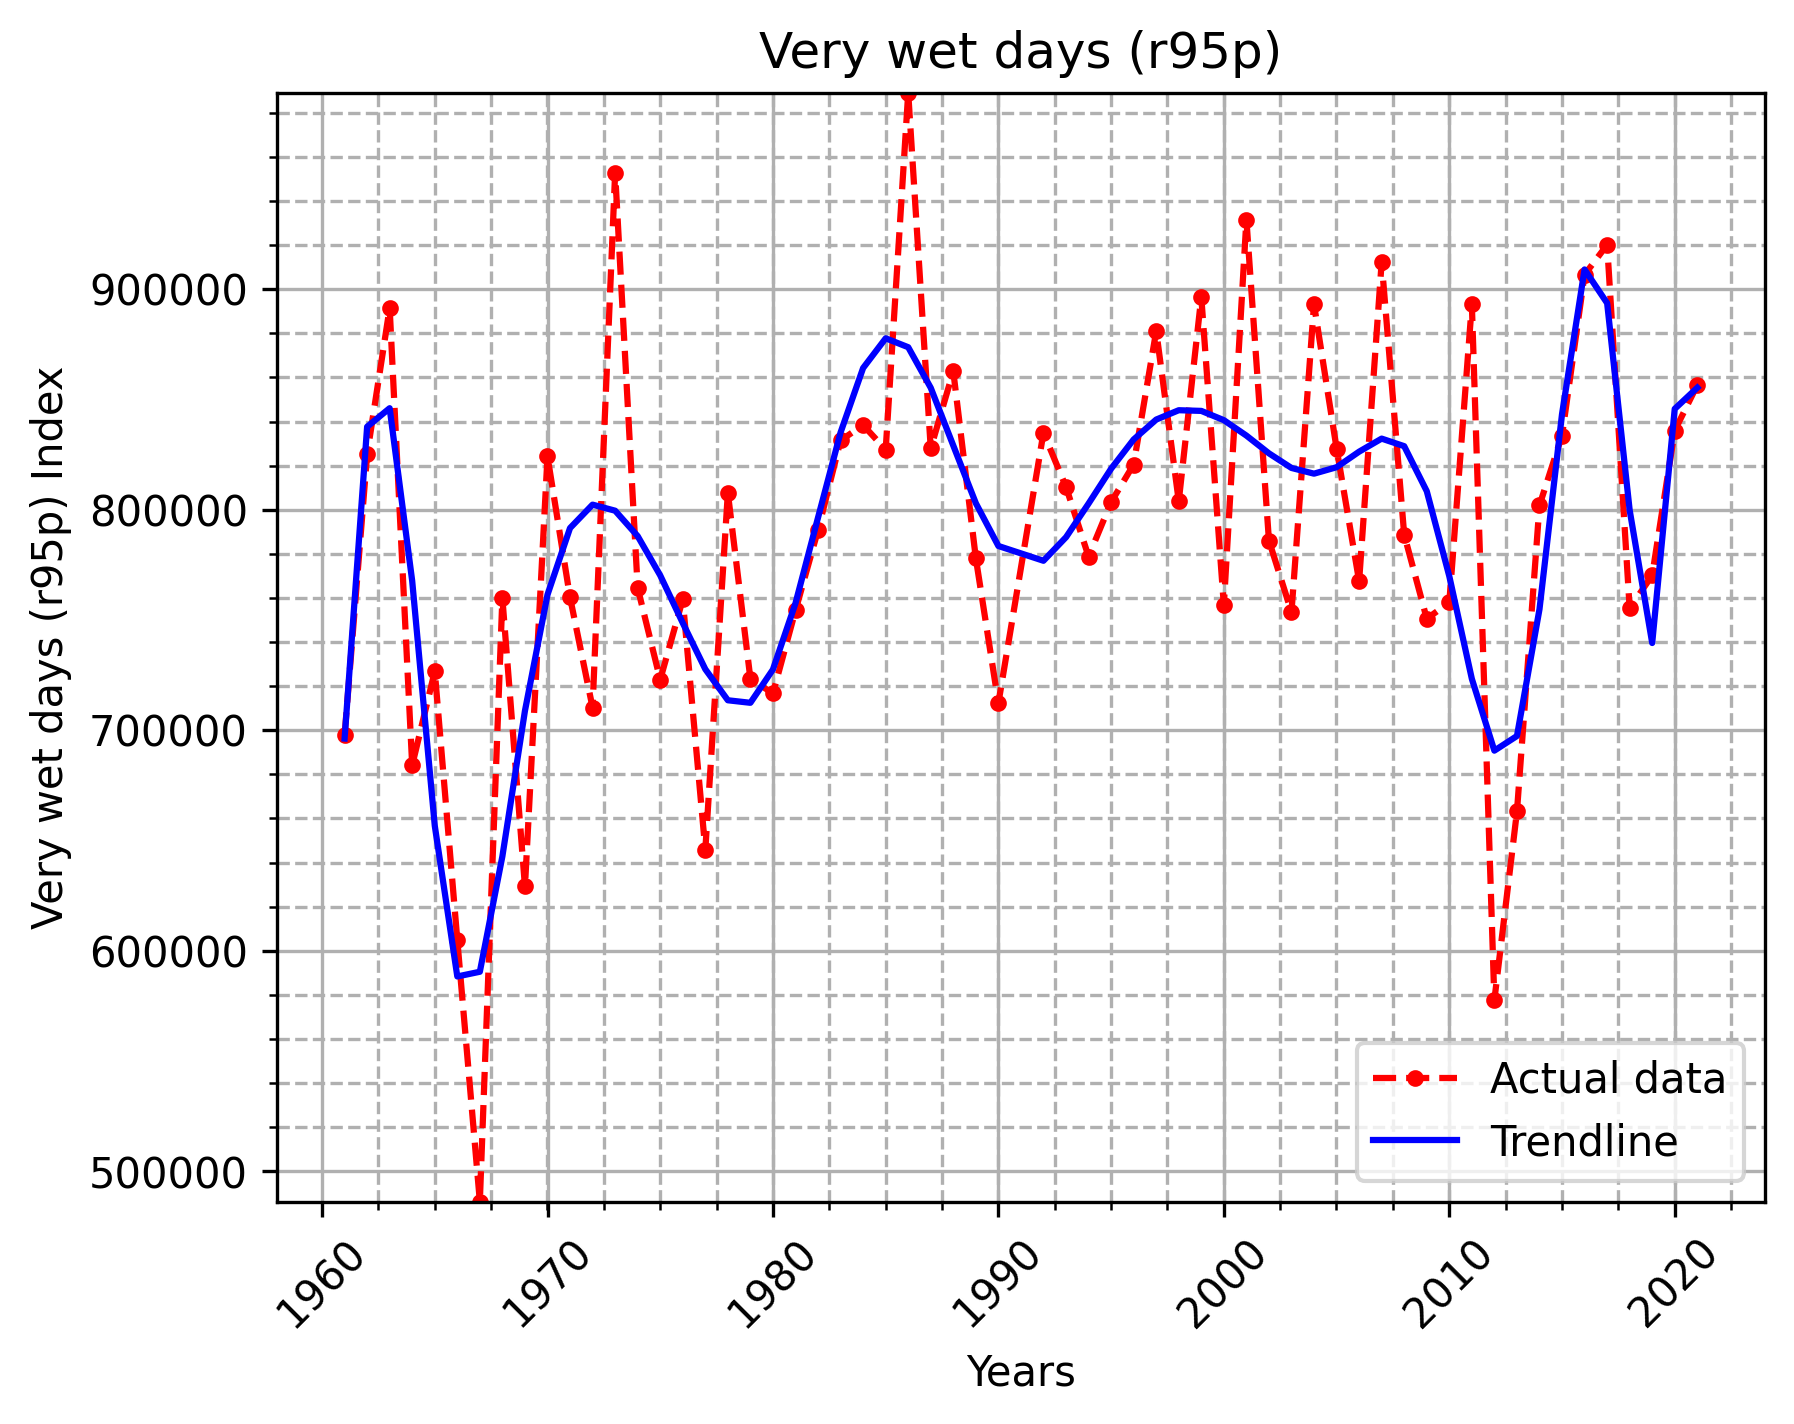
\includegraphics[width=0.75\textwidth]{//home/shiv/Documents/GitHub/EES405/clim_indices/final_plots/r95p.png}
    \caption{Very wet days (R95p) temporal Plot}
    \label{fig:r95p_temporal}
\end{figure}

$ y = -3.42\times10^{3}x^{21}+7.44\times10^{-5}x^{20}-1.88\times10^{-6}x^{19}+3.31\times10^{-10}x^{18}+1.08\times10^{-12}x^{17}-3.97\times10^{-16}x^{16}-1.62\times10^{-19}x^{15}+1.05\times10^{-22}x^{14}-5.80\times10^{-27}x^{13}-8.00\times10^{-30}x^{12}+2.29\times10^{-33}x^{11}-1.20\times10^{-37}x^{10}-6.72\times10^{-41}x^{9}+1.99\times10^{-44}x^{8}-2.95\times10^{-48}x^{7}+2.85\times10^{-52}x^{6}-1.92\times10^{-56}x^{5}+9.12\times10^{-61}x^{4}-3.03\times10^{-65}x^{3}+6.69\times10^{-70}x^{2}-8.87\times10^{-75}x+5.34\times10^{-80}$

The incease in the frequency of very wet days is consistent with the overall warming of the planet due to climate change as seen in the above spatial plot.\\
Overall, the increase in the frequency of cold nights is a consistent and expected result of the overall warming of the planet due to climate change.

\section {Consecutive dry days}
% \newpage
\subsection {Spatial plot for consecutive dry days (CDD)}
\begin{figure}[htb]
    \centering
    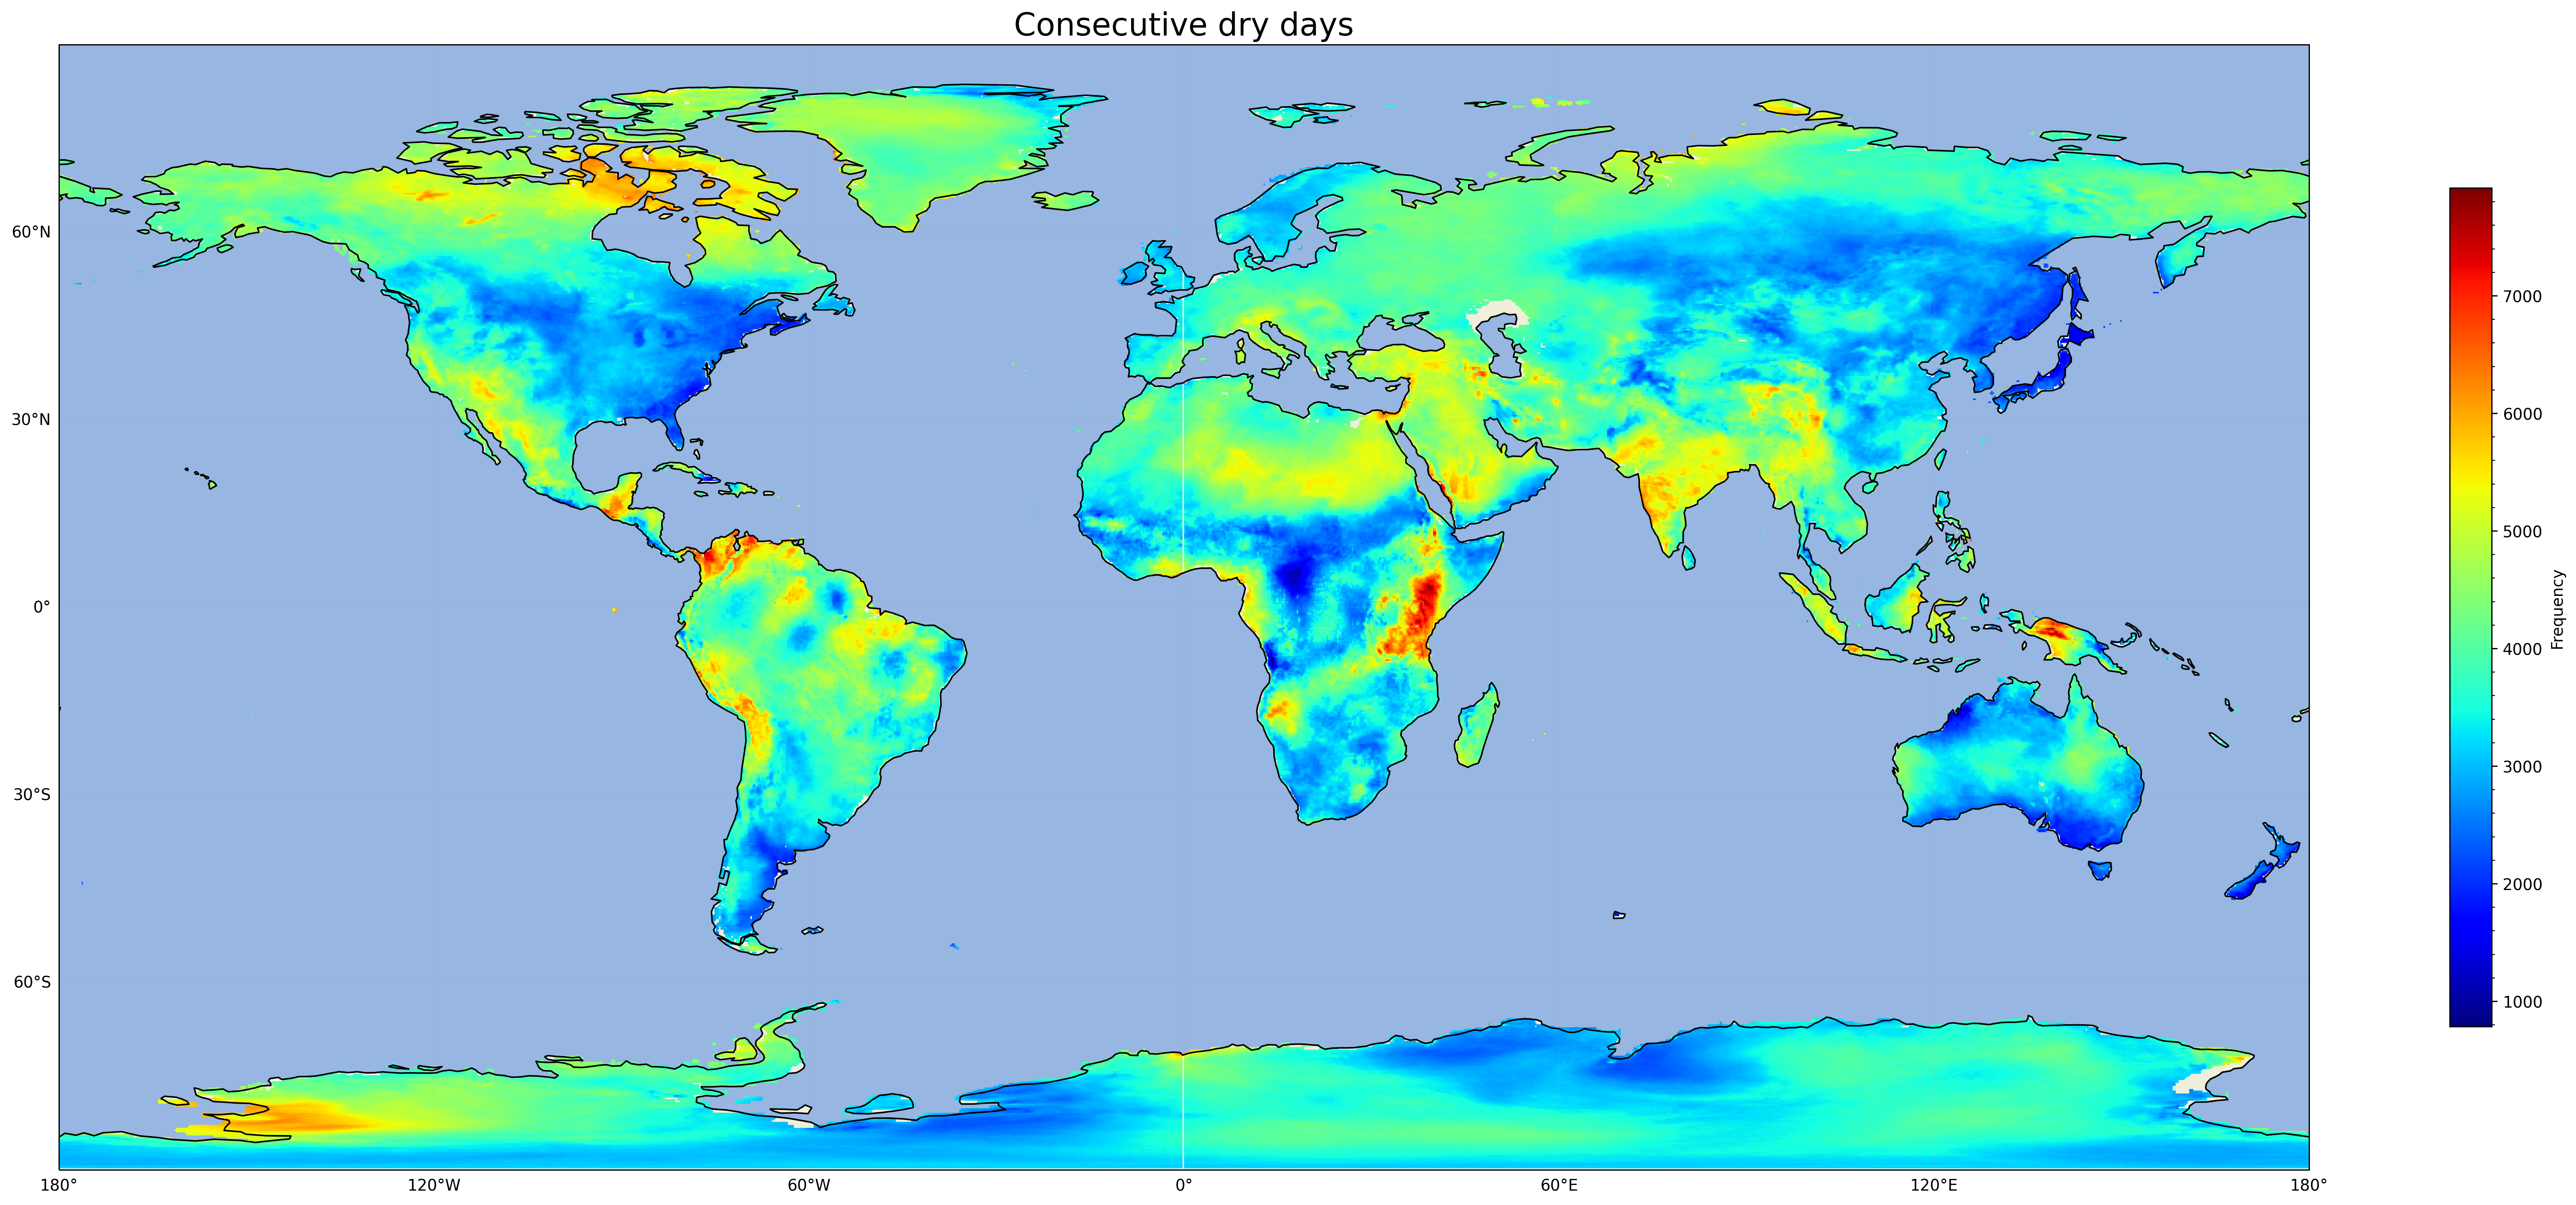
\includegraphics[width=0.80\textwidth]{/home/shiv/Documents/GitHub/EES405/clim_indices/final_plots/cdd-spatial.png}
    \caption{CD days Spatial Plot}
    \label{fig:cdd_spatial}
\end{figure}

\subsection{Temporal Plot for 'Consecutive dry days (CDD)'}
In the above time series plot of heavy precipitation days anomalies calculated from the \textbf{CDD} climate index, we have added a non-linear trendline with polynomial fit of degree 21 (as used in the paper by )given by the following equation.
\begin{figure}[htb]
    \centering
    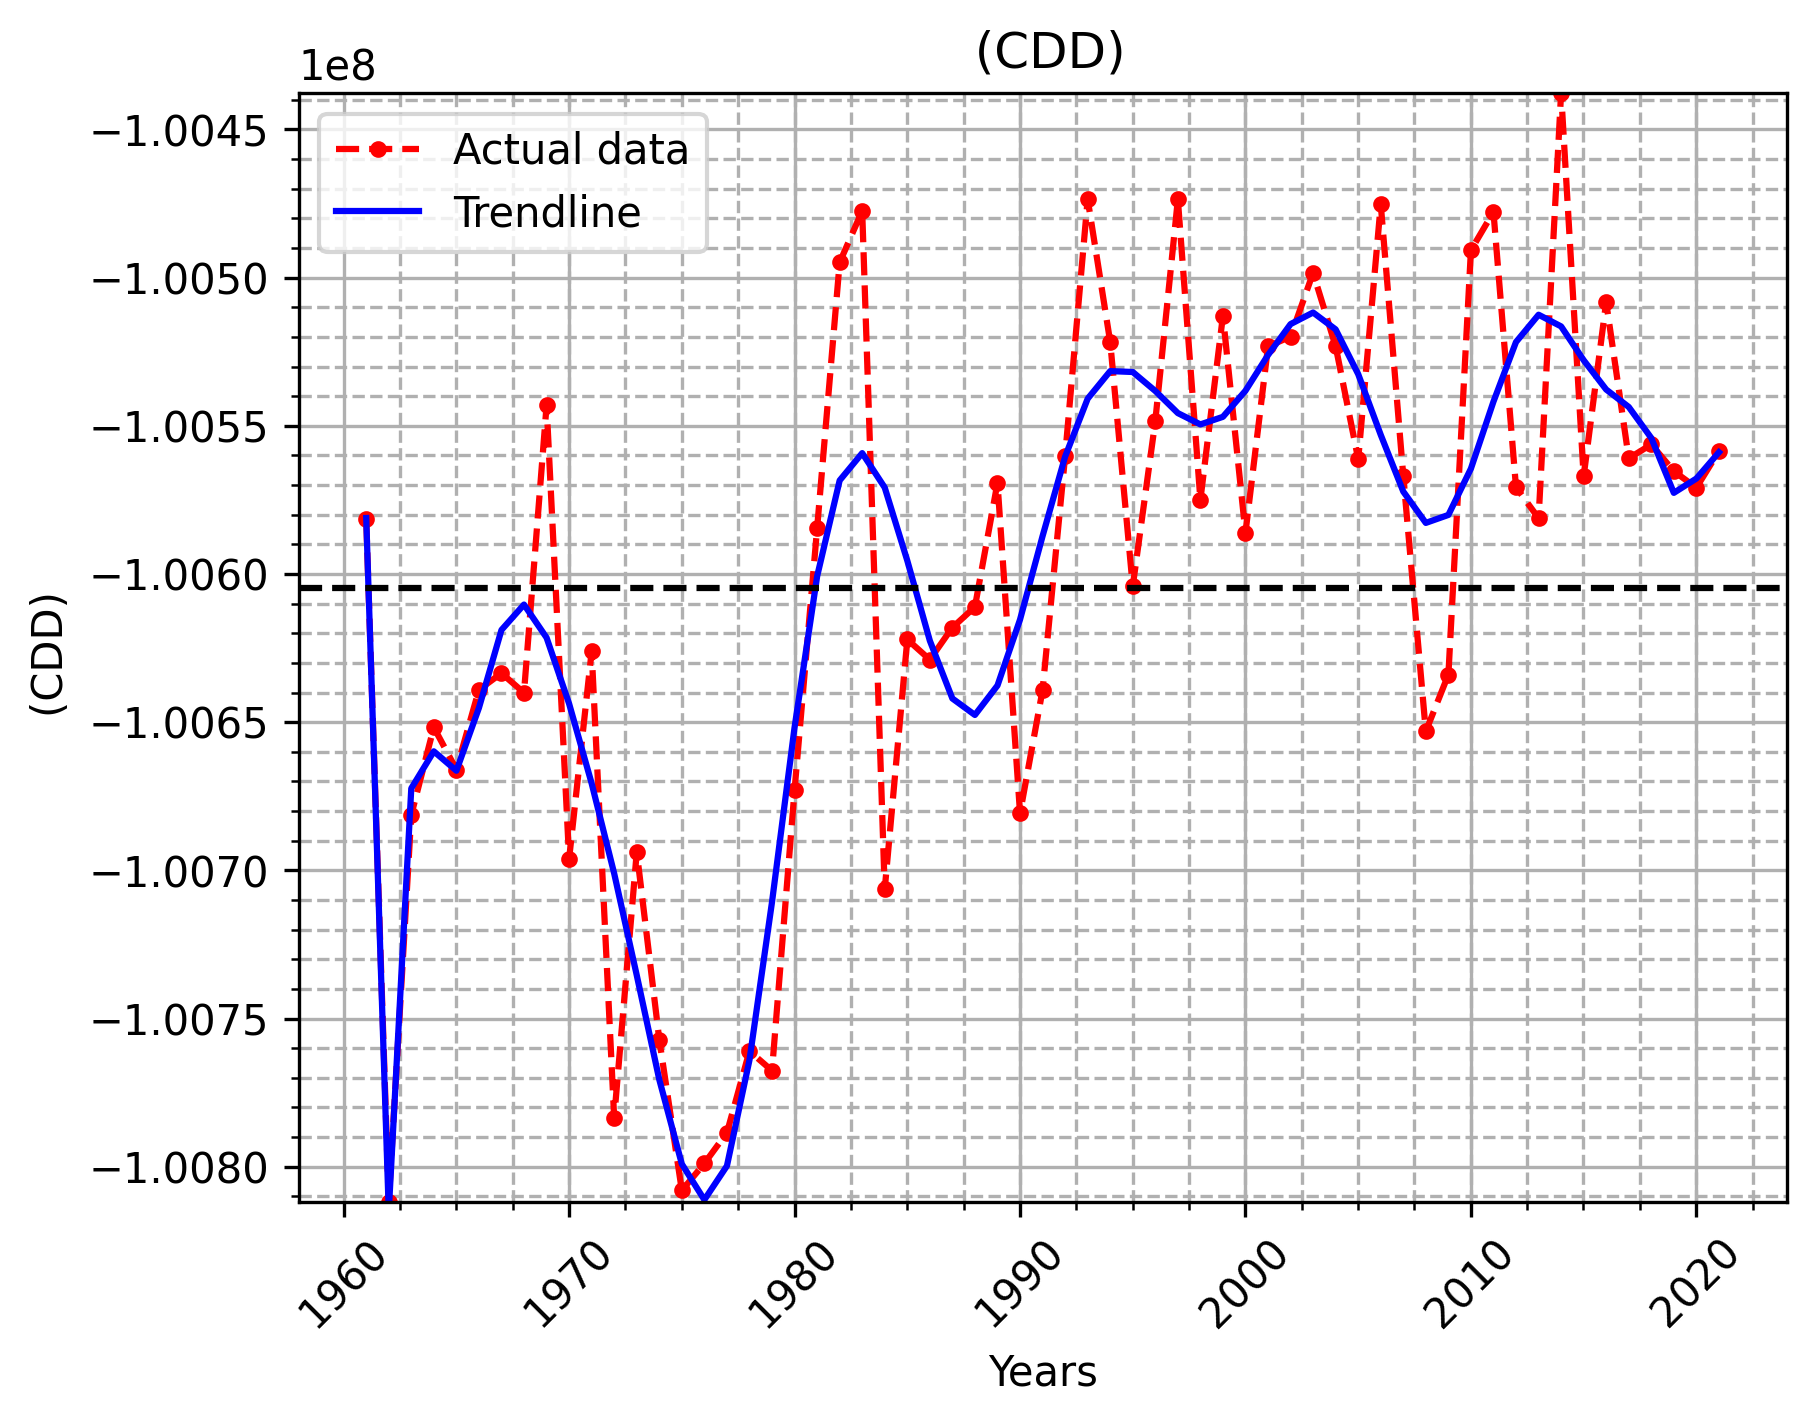
\includegraphics[width=0.75\textwidth]{/home/shiv/Documents/GitHub/EES405/clim_indices/final_plots/cdd-time.png}
    \caption{Consecutive dry days (CDD) temporal Plot}
    \label{fig:cdd_temporal}
\end{figure}

$ y = -3.42\times10^{3}x^{21}+7.44\times10^{-5}x^{20}-1.88\times10^{-6}x^{19}+3.31\times10^{-10}x^{18}+1.08\times10^{-12}x^{17}-3.97\times10^{-16}x^{16}-1.62\times10^{-19}x^{15}+1.05\times10^{-22}x^{14}-5.80\times10^{-27}x^{13}-8.00\times10^{-30}x^{12}+2.29\times10^{-33}x^{11}-1.20\times10^{-37}x^{10}-6.72\times10^{-41}x^{9}+1.99\times10^{-44}x^{8}-2.95\times10^{-48}x^{7}+2.85\times10^{-52}x^{6}-1.92\times10^{-56}x^{5}+9.12\times10^{-61}x^{4}-3.03\times10^{-65}x^{3}+6.69\times10^{-70}x^{2}-8.87\times10^{-75}x+5.34\times10^{-80}$

The incease in the frequency of consecutive dry days is consistent with the overall warming of the planet due to climate change as seen in the above spatial plot.\\
Overall, the increase in the frequency of cold nights is a consistent and expected result of the overall warming of the planet due to climate change.

\section {Daily Intensity}
% \subsection{Spatial plot for daily intensity (SDII)}
% \begin{figure}[htb]
%     \centering
%     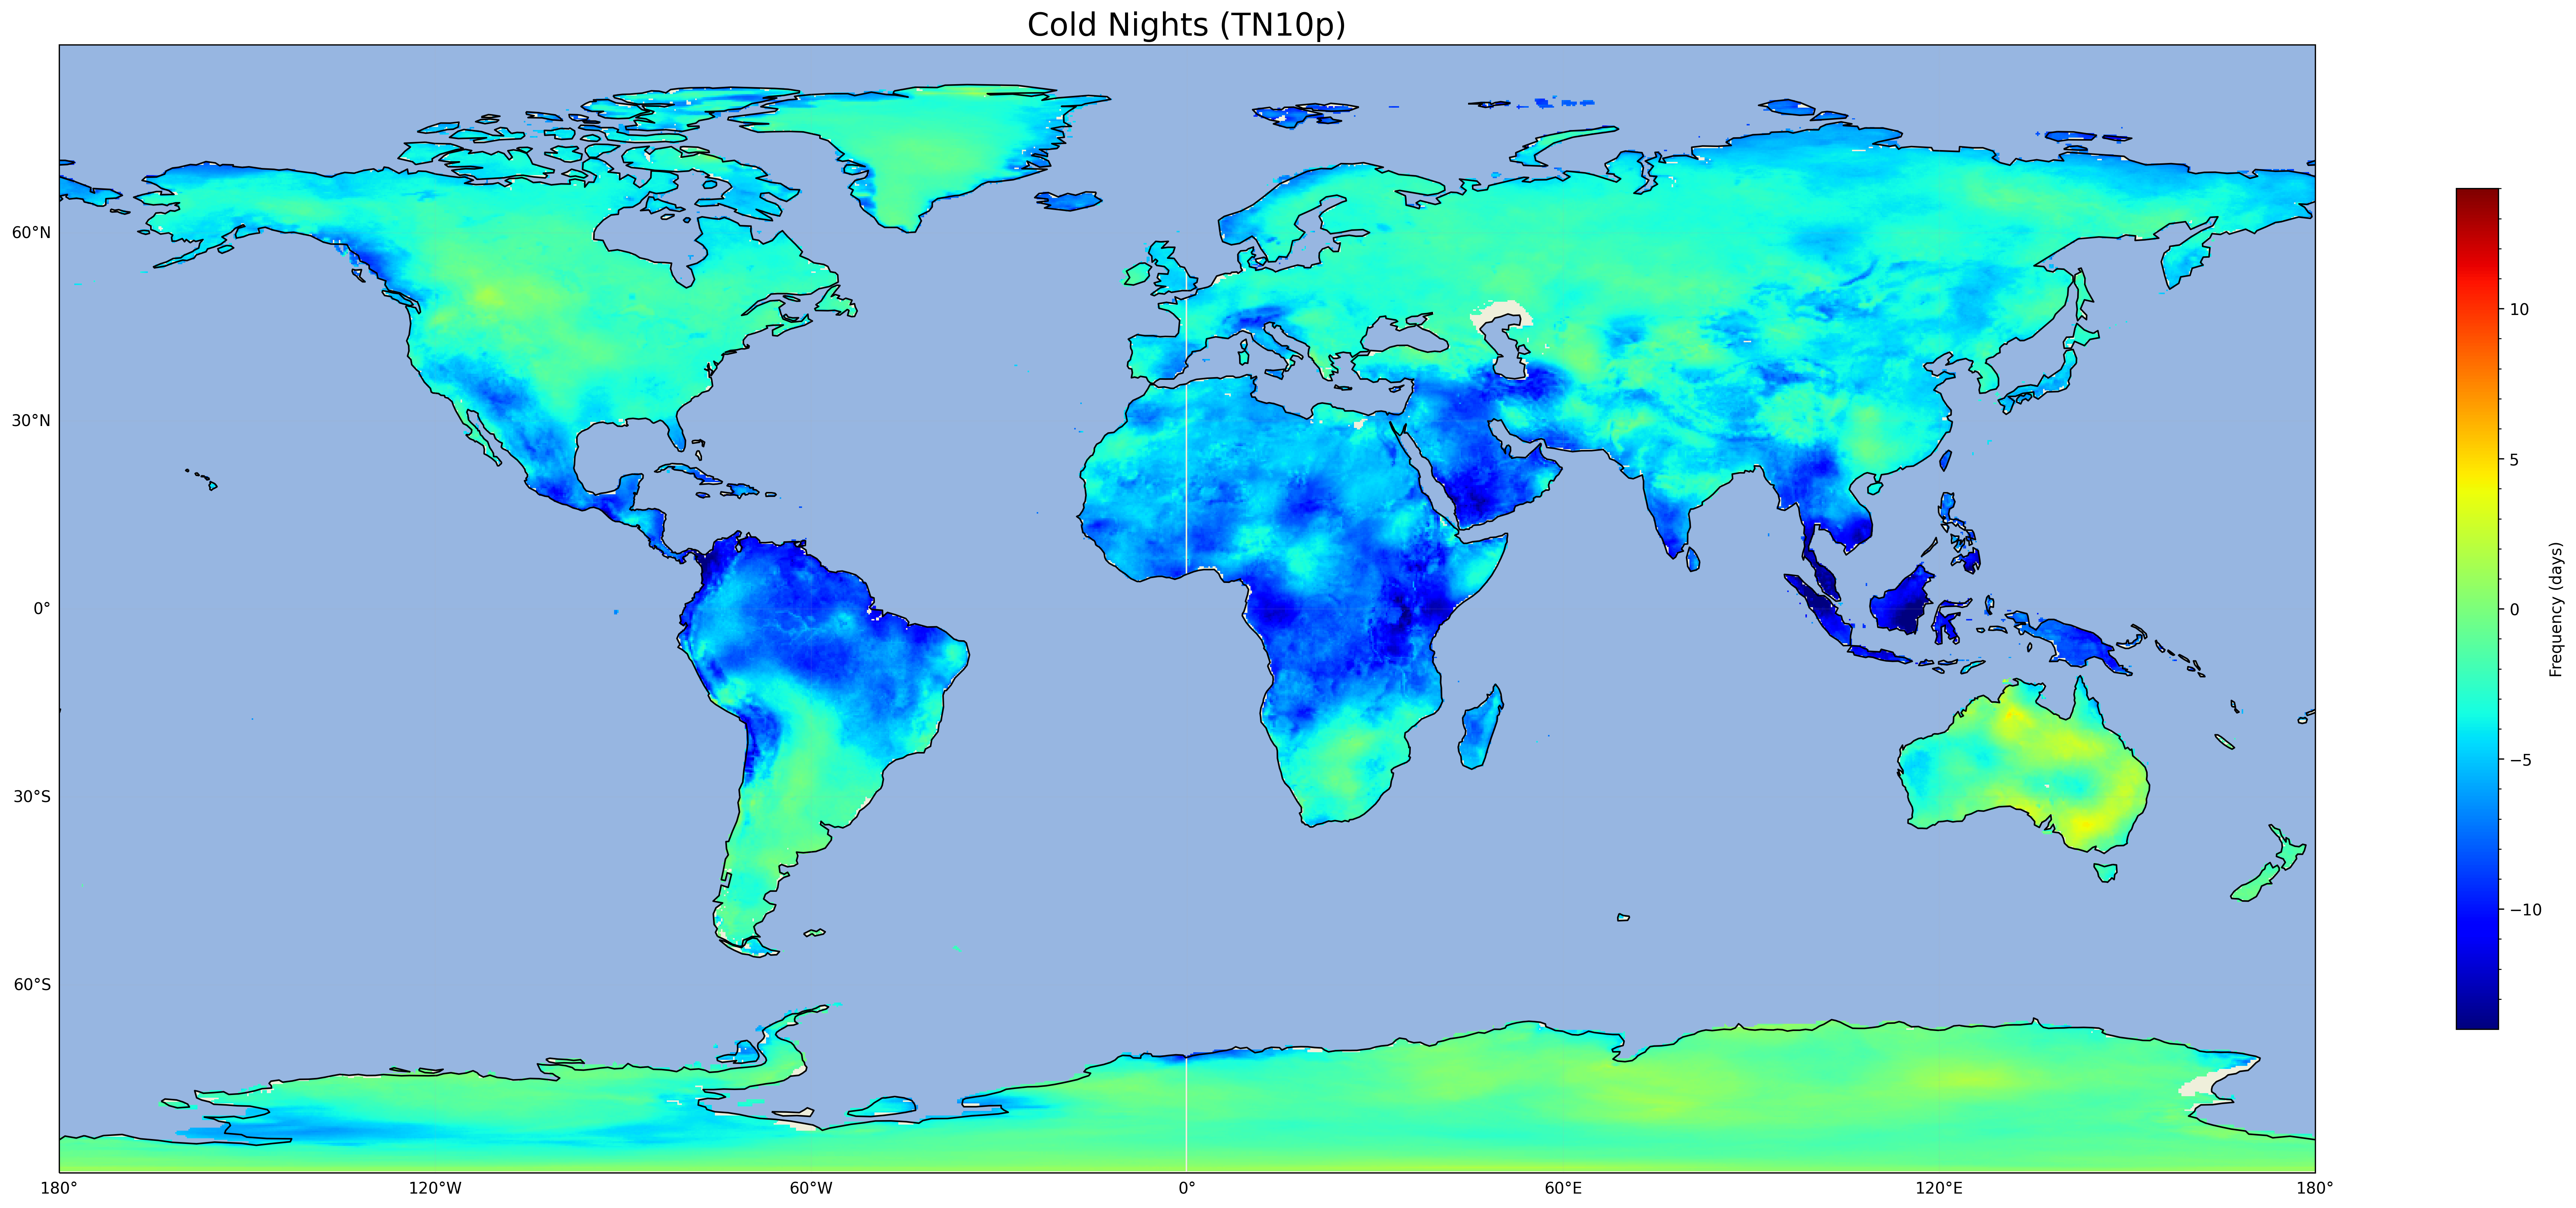
\includegraphics[width=0.80\textwidth]{/home/shiv/Documents/GitHub/EES405/clim_extreme/plots_clim_extreme/cold_nights.png}
%     \caption{Warm days Spatial Plot}
%     \label{fig:sdii_spatial}
% \end{figure}

\subsection{Temporal Plot for 'Simple daily intensity (SDII)'}
In the above time series plot of simple daily intensity anomalies calculated from the \textbf{SDII} climate index, we have added a non-linear trendline with polynomial fit of degree 21 (as used in the paper by )given by the following equation.\\

\begin{figure}[htb]
    \centering
    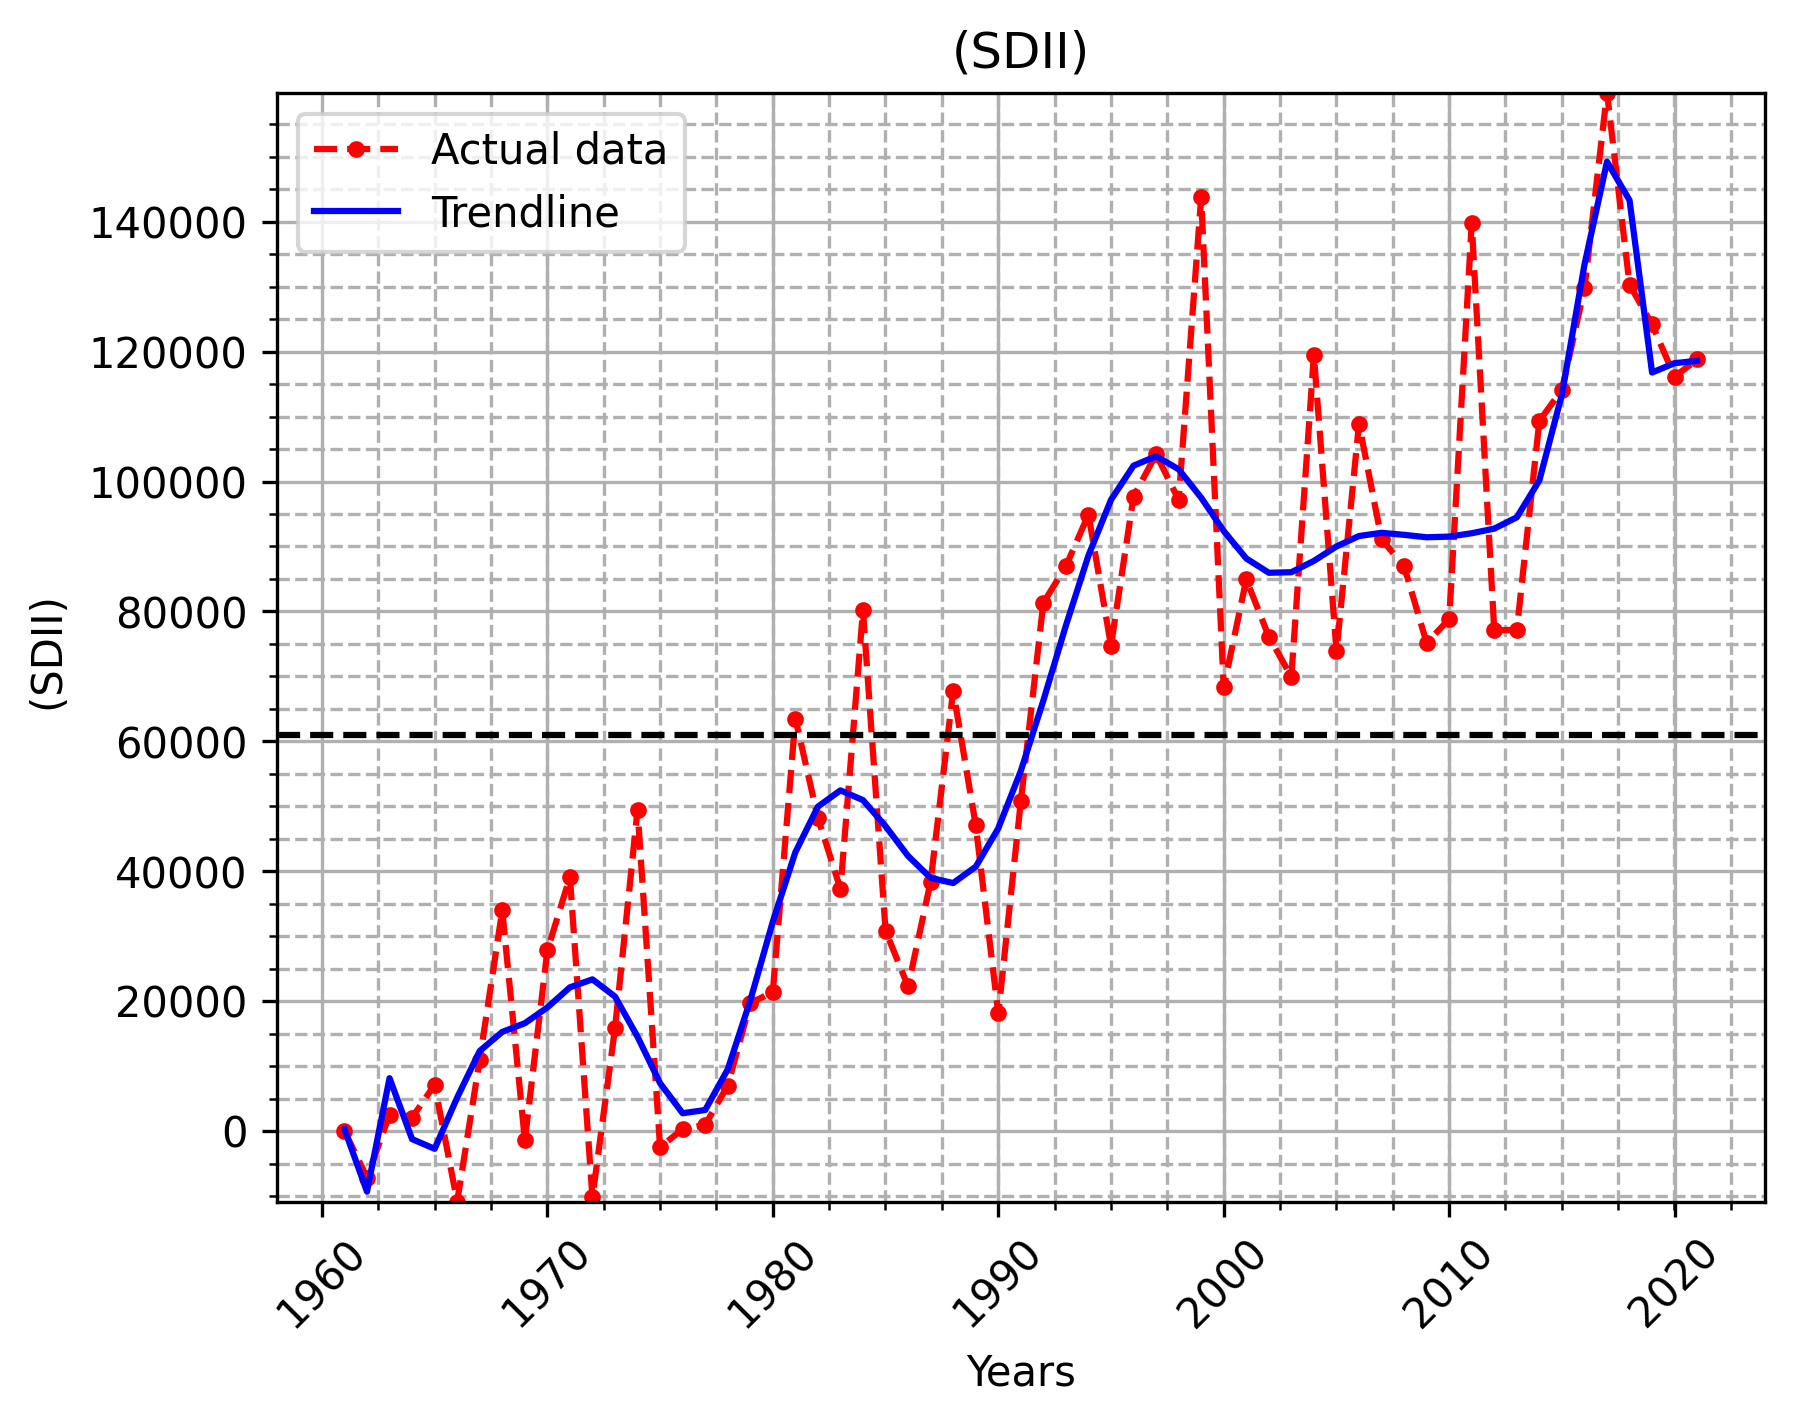
\includegraphics[width=0.75\textwidth]{//home/shiv/Documents/GitHub/EES405/clim_indices/final_plots/sdii-time.png}
    \caption{Simple daily intensity (SDII) temporal Plot}
    \label{fig:sdii_temporal}
\end{figure}

$ y = -3.42\times10^{3}x^{21}+7.44\times10^{-5}x^{20}-1.88\times10^{-6}x^{19}+3.31\times10^{-10}x^{18}+1.08\times10^{-12}x^{17}-3.97\times10^{-16}x^{16}-1.62\times10^{-19}x^{15}+1.05\times10^{-22}x^{14}-5.80\times10^{-27}x^{13}-8.00\times10^{-30}x^{12}+2.29\times10^{-33}x^{11}-1.20\times10^{-37}x^{10}-6.72\times10^{-41}x^{9}+1.99\times10^{-44}x^{8}-2.95\times10^{-48}x^{7}+2.85\times10^{-52}x^{6}-1.92\times10^{-56}x^{5}+9.12\times10^{-61}x^{4}-3.03\times10^{-65}x^{3}+6.69\times10^{-70}x^{2}-8.87\times10^{-75}x+5.34\times10^{-80}$

The incease in the frequency of simple daily intensity is consistent with the overall warming of the planet due to climate change as seen in the above spatial plot.\\
Overall, the increase in the frequency of cold nights is a consistent and expected result of the overall warming of the planet due to climate change.

\section{Seasonal maximum 5-day precipitation amount(RX5day)}
% \subsection{Spatial plot for 5-day precipitation amount (RX5) for DJF season}
% \begin{figure}[htb]
%     \centering
%     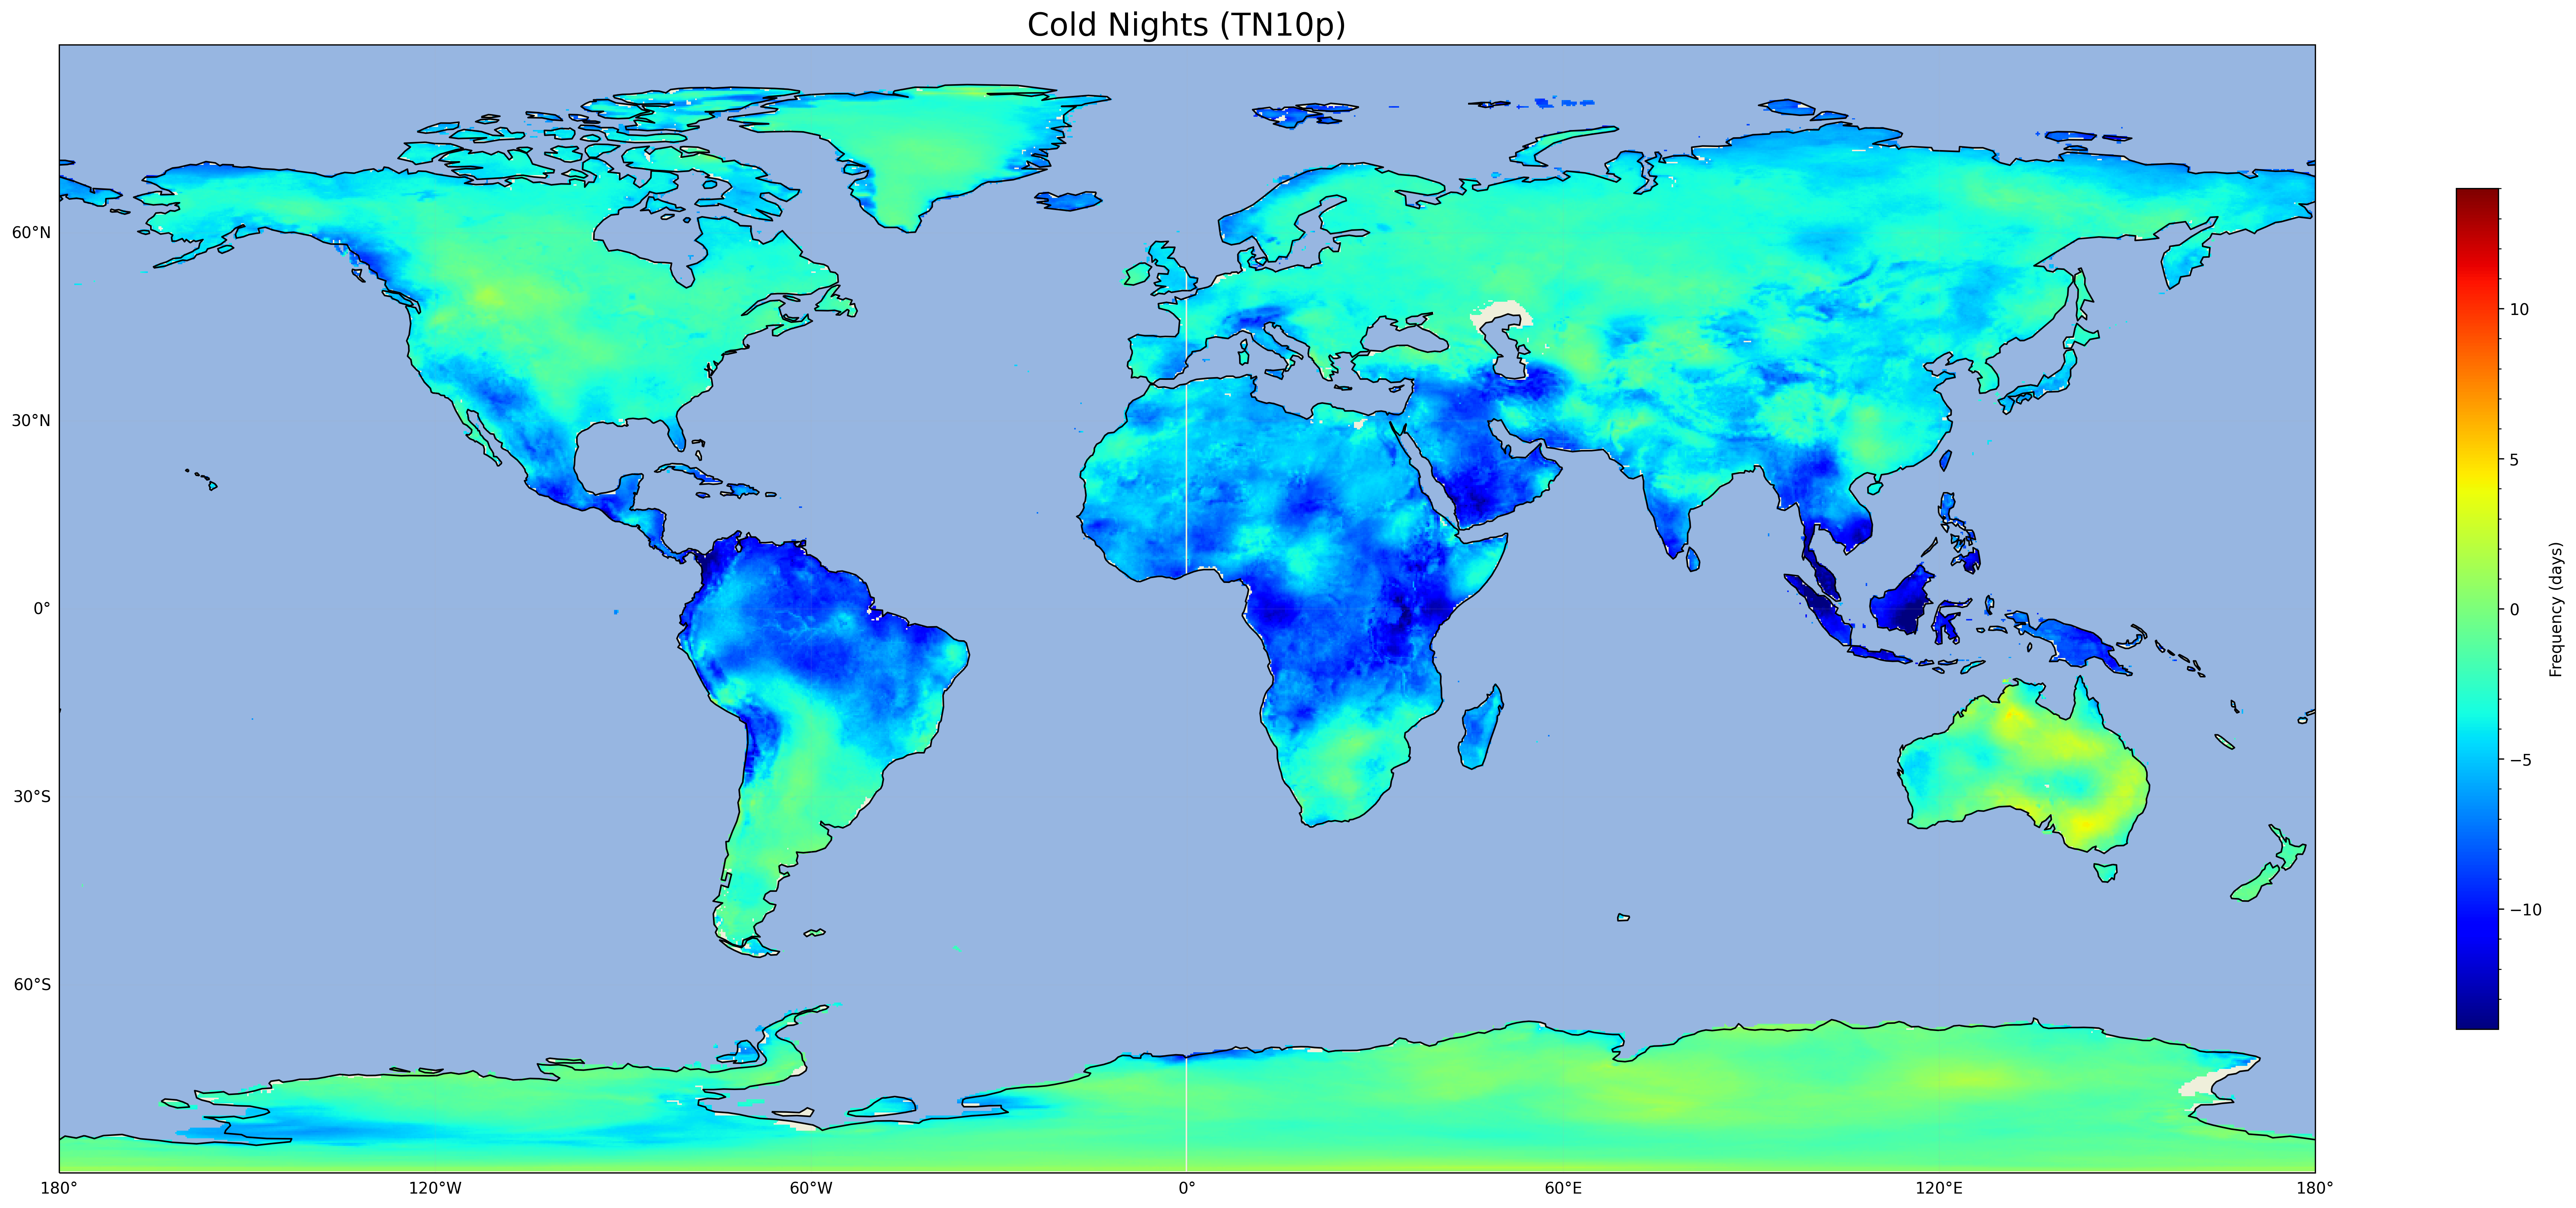
\includegraphics[width=0.80\textwidth]{/home/shiv/Documents/GitHub/EES405/clim_extreme/plots_clim_extreme/cold_nights.png}
%     \caption{Warm days Spatial Plot}
%     \label{fig:rx5_djf_spatial}
% \end{figure}

\subsection{Temporal Plot for '5-day precipitation amount (RX5) for DJF season'}
In the above time series plot of 5-day precipitation amount anomalies for (DJF) months calculated from the \textbf{RX5} climate index, we have added a non-linear trendline with polynomial fit of degree 21 (as used in the paper by )given by the following equation.
\begin{figure}[htb]
    \centering
    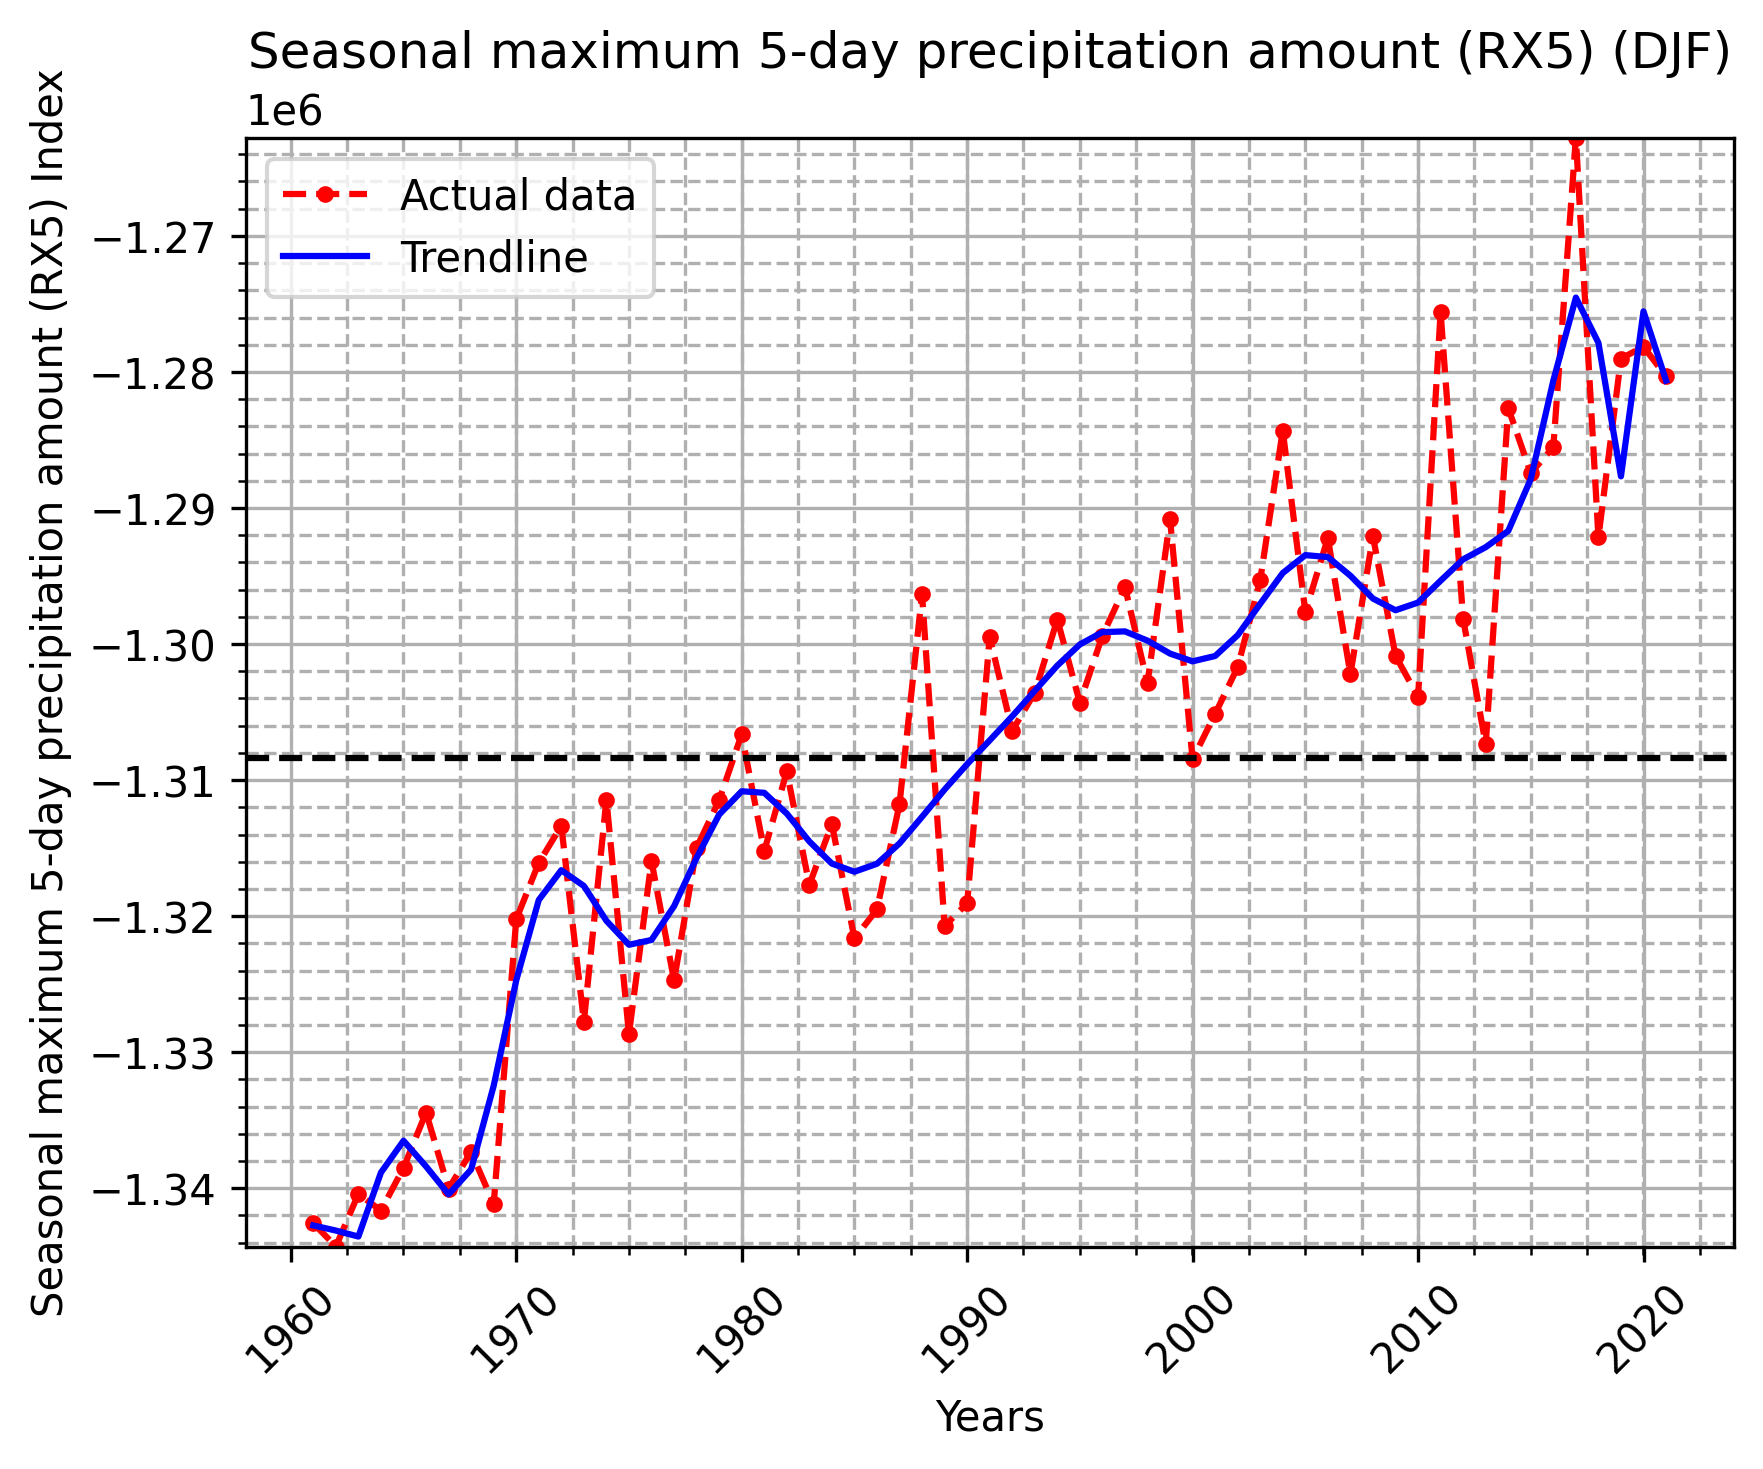
\includegraphics[width=0.75\textwidth]{//home/shiv/Documents/GitHub/EES405/clim_indices/final_plots/rx5_djf.png}
    \caption{5-day precipitation amount (RX5) (DJF) temporal Plot}
    \label{fig:rx5_djf_temporal}
\end{figure}

$ y = -3.42\times10^{3}x^{21}+7.44\times10^{-5}x^{20}-1.88\times10^{-6}x^{19}+3.31\times10^{-10}x^{18}+1.08\times10^{-12}x^{17}-3.97\times10^{-16}x^{16}-1.62\times10^{-19}x^{15}+1.05\times10^{-22}x^{14}-5.80\times10^{-27}x^{13}-8.00\times10^{-30}x^{12}+2.29\times10^{-33}x^{11}-1.20\times10^{-37}x^{10}-6.72\times10^{-41}x^{9}+1.99\times10^{-44}x^{8}-2.95\times10^{-48}x^{7}+2.85\times10^{-52}x^{6}-1.92\times10^{-56}x^{5}+9.12\times10^{-61}x^{4}-3.03\times10^{-65}x^{3}+6.69\times10^{-70}x^{2}-8.87\times10^{-75}x+5.34\times10^{-80}$

The incease in the frequency of 5-day precipitation amount is consistent with the overall warming of the planet due to climate change as seen in the above spatial plot.\\
Overall, the increase in the frequency of 5-day precipitation amount is a consistent and expected result of the overall warming of the planet due to climate change.
\newpage
% \subsection{Spatial plot for 5-day precipitation amount (RX5) for MAM season}
% \begin{figure}[htb]
%     \centering
%     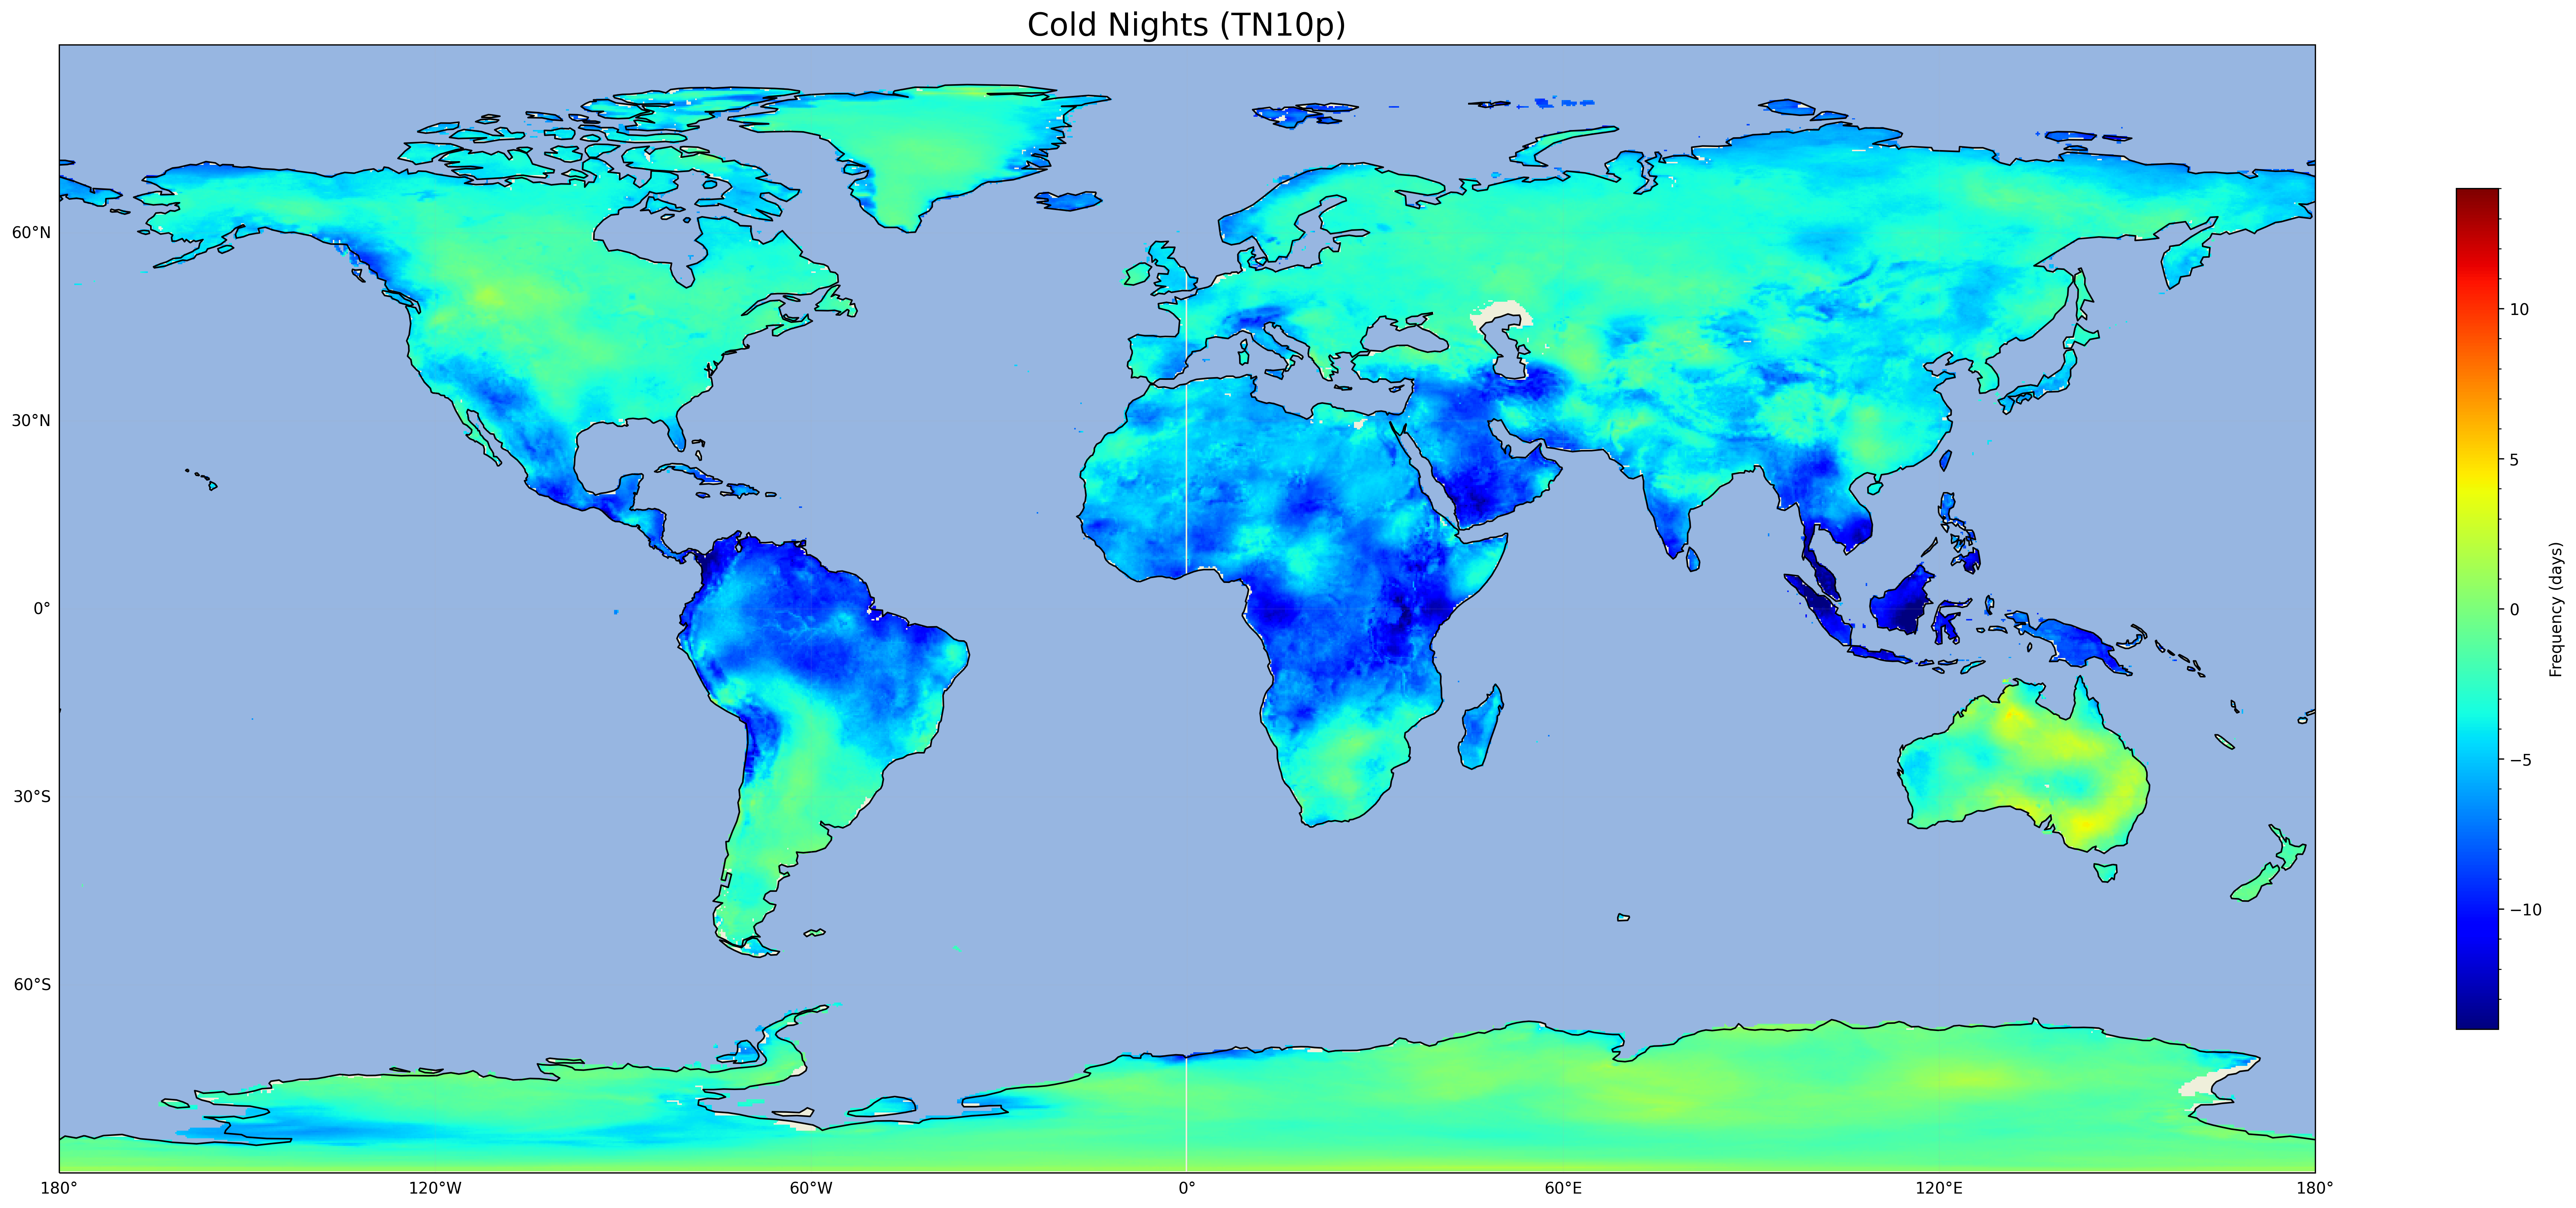
\includegraphics[width=0.80\textwidth]{/home/shiv/Documents/GitHub/EES405/clim_extreme/plots_clim_extreme/cold_nights.png}
%     \caption{Warm days Spatial Plot}
%     \label{fig:rx5_mam_spatial}
% \end{figure}

\subsection{Temporal Plot for '5-day precipitation amount (RX5) for MAM season'}
In the above time series plot of 5-day precipitation amount anomalies for (MAM) months calculated from the \textbf{RX5} climate index, we have added a non-linear trendline with polynomial fit of degree 21 (as used in the paper by )given by the following equation.
\begin{figure}[htb]
    \centering
    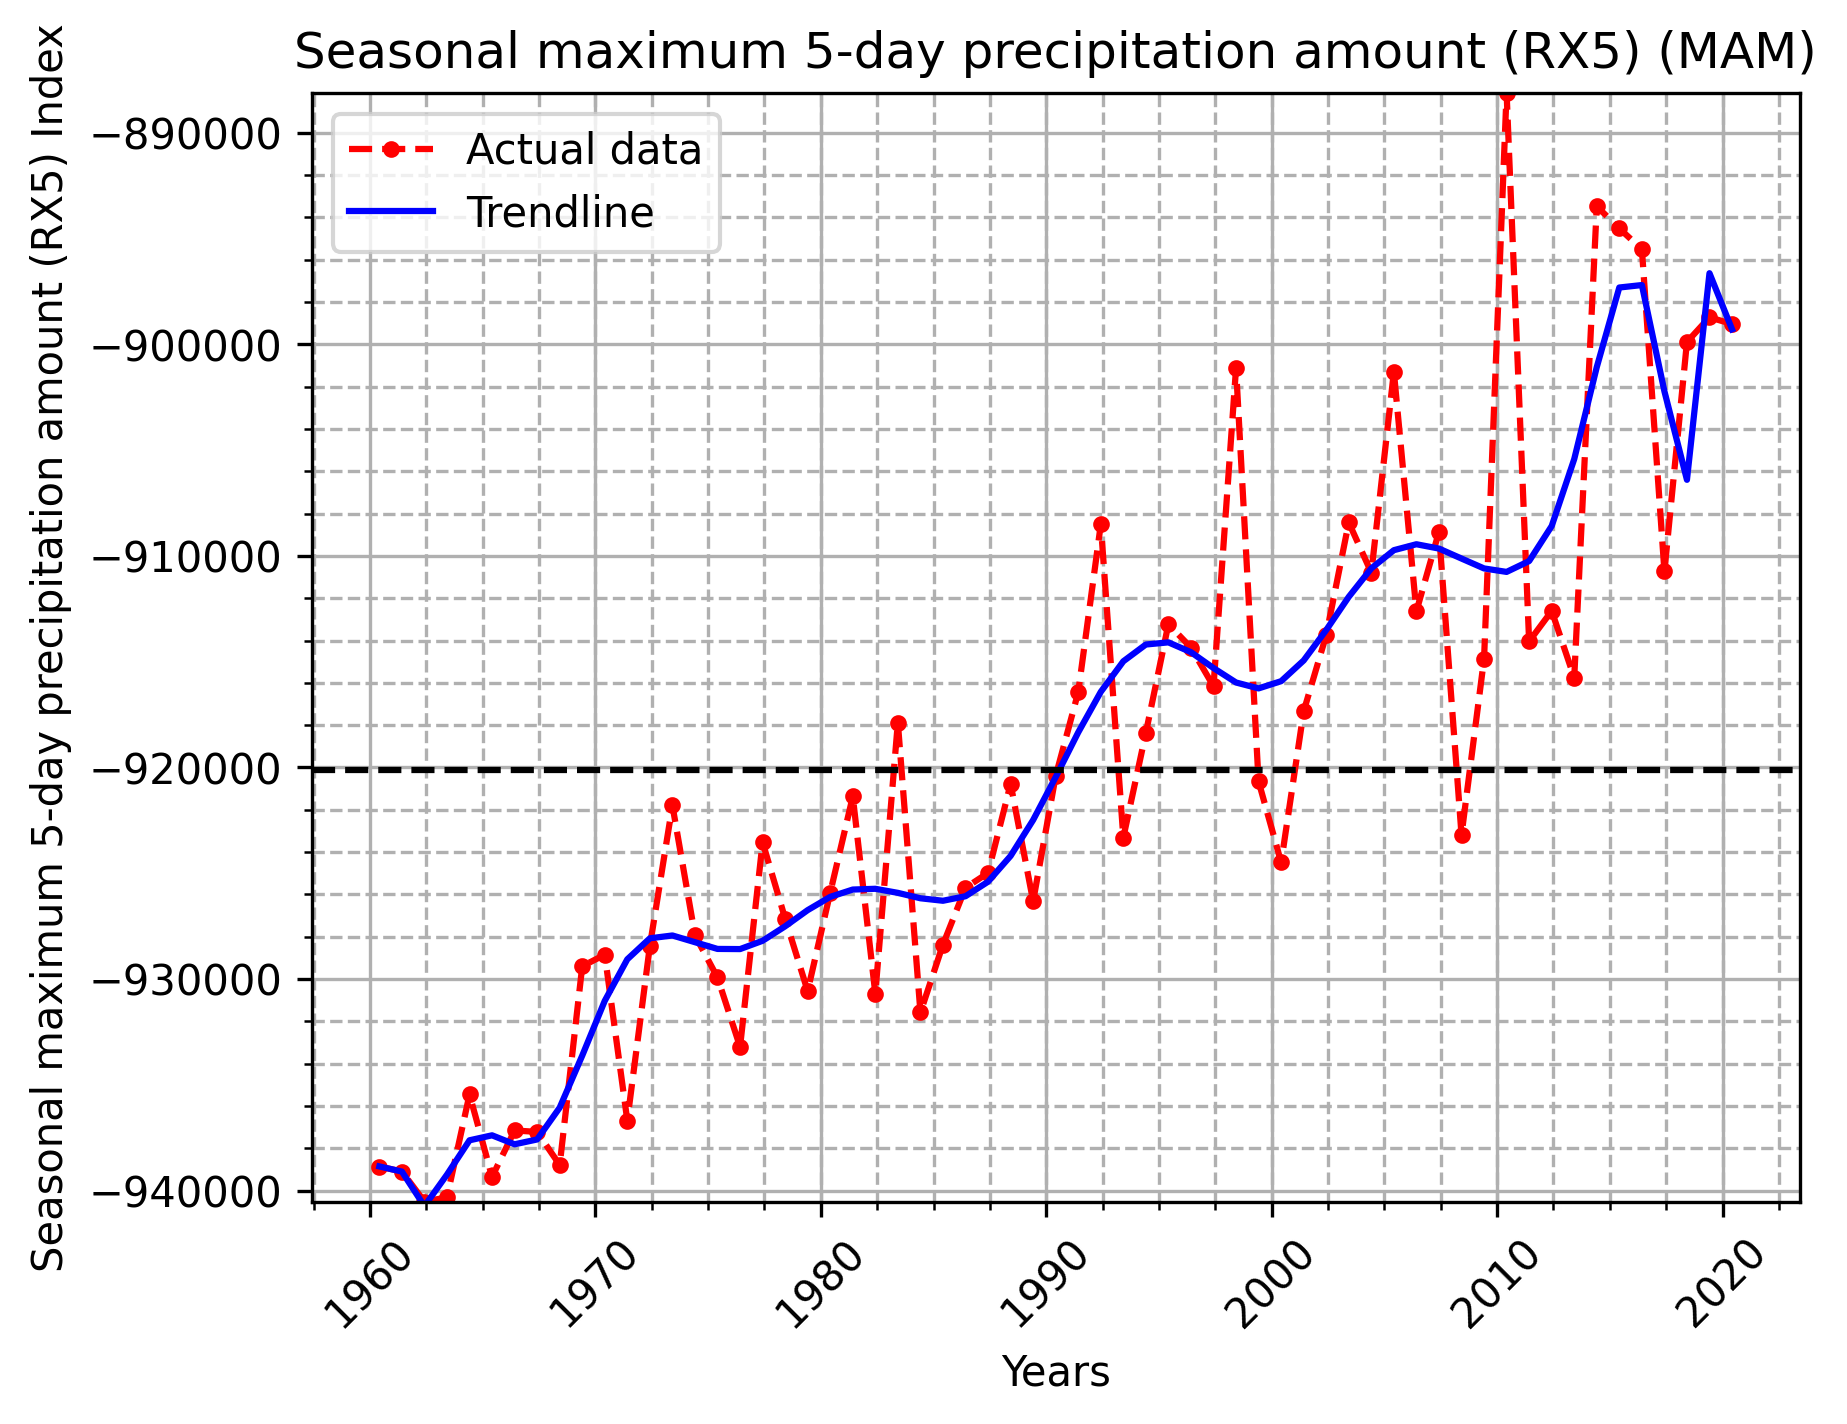
\includegraphics[width=0.75\textwidth]{//home/shiv/Documents/GitHub/EES405/clim_indices/final_plots/rx5_mam.png}
    \caption{5-day precipitation amount (RX5) (MAM) temporal Plot}
    \label{fig:rx5_mam_temporal}
\end{figure}

$ y = -3.42\times10^{3}x^{21}+7.44\times10^{-5}x^{20}-1.88\times10^{-6}x^{19}+3.31\times10^{-10}x^{18}+1.08\times10^{-12}x^{17}-3.97\times10^{-16}x^{16}-1.62\times10^{-19}x^{15}+1.05\times10^{-22}x^{14}-5.80\times10^{-27}x^{13}-8.00\times10^{-30}x^{12}+2.29\times10^{-33}x^{11}-1.20\times10^{-37}x^{10}-6.72\times10^{-41}x^{9}+1.99\times10^{-44}x^{8}-2.95\times10^{-48}x^{7}+2.85\times10^{-52}x^{6}-1.92\times10^{-56}x^{5}+9.12\times10^{-61}x^{4}-3.03\times10^{-65}x^{3}+6.69\times10^{-70}x^{2}-8.87\times10^{-75}x+5.34\times10^{-80}$

The incease in the frequency of 5-day precipitation amount is consistent with the overall warming of the planet due to climate change as seen in the above spatial plot.\\
Overall, the increase in the frequency of 5-day precipitation amount is a consistent and expected result of the overall warming of the planet due to climate change.

% \subsection{Spatial plot for 5-day precipitation amount (RX5) for JJA season}
% \begin{figure}[htb]
%     \centering
%     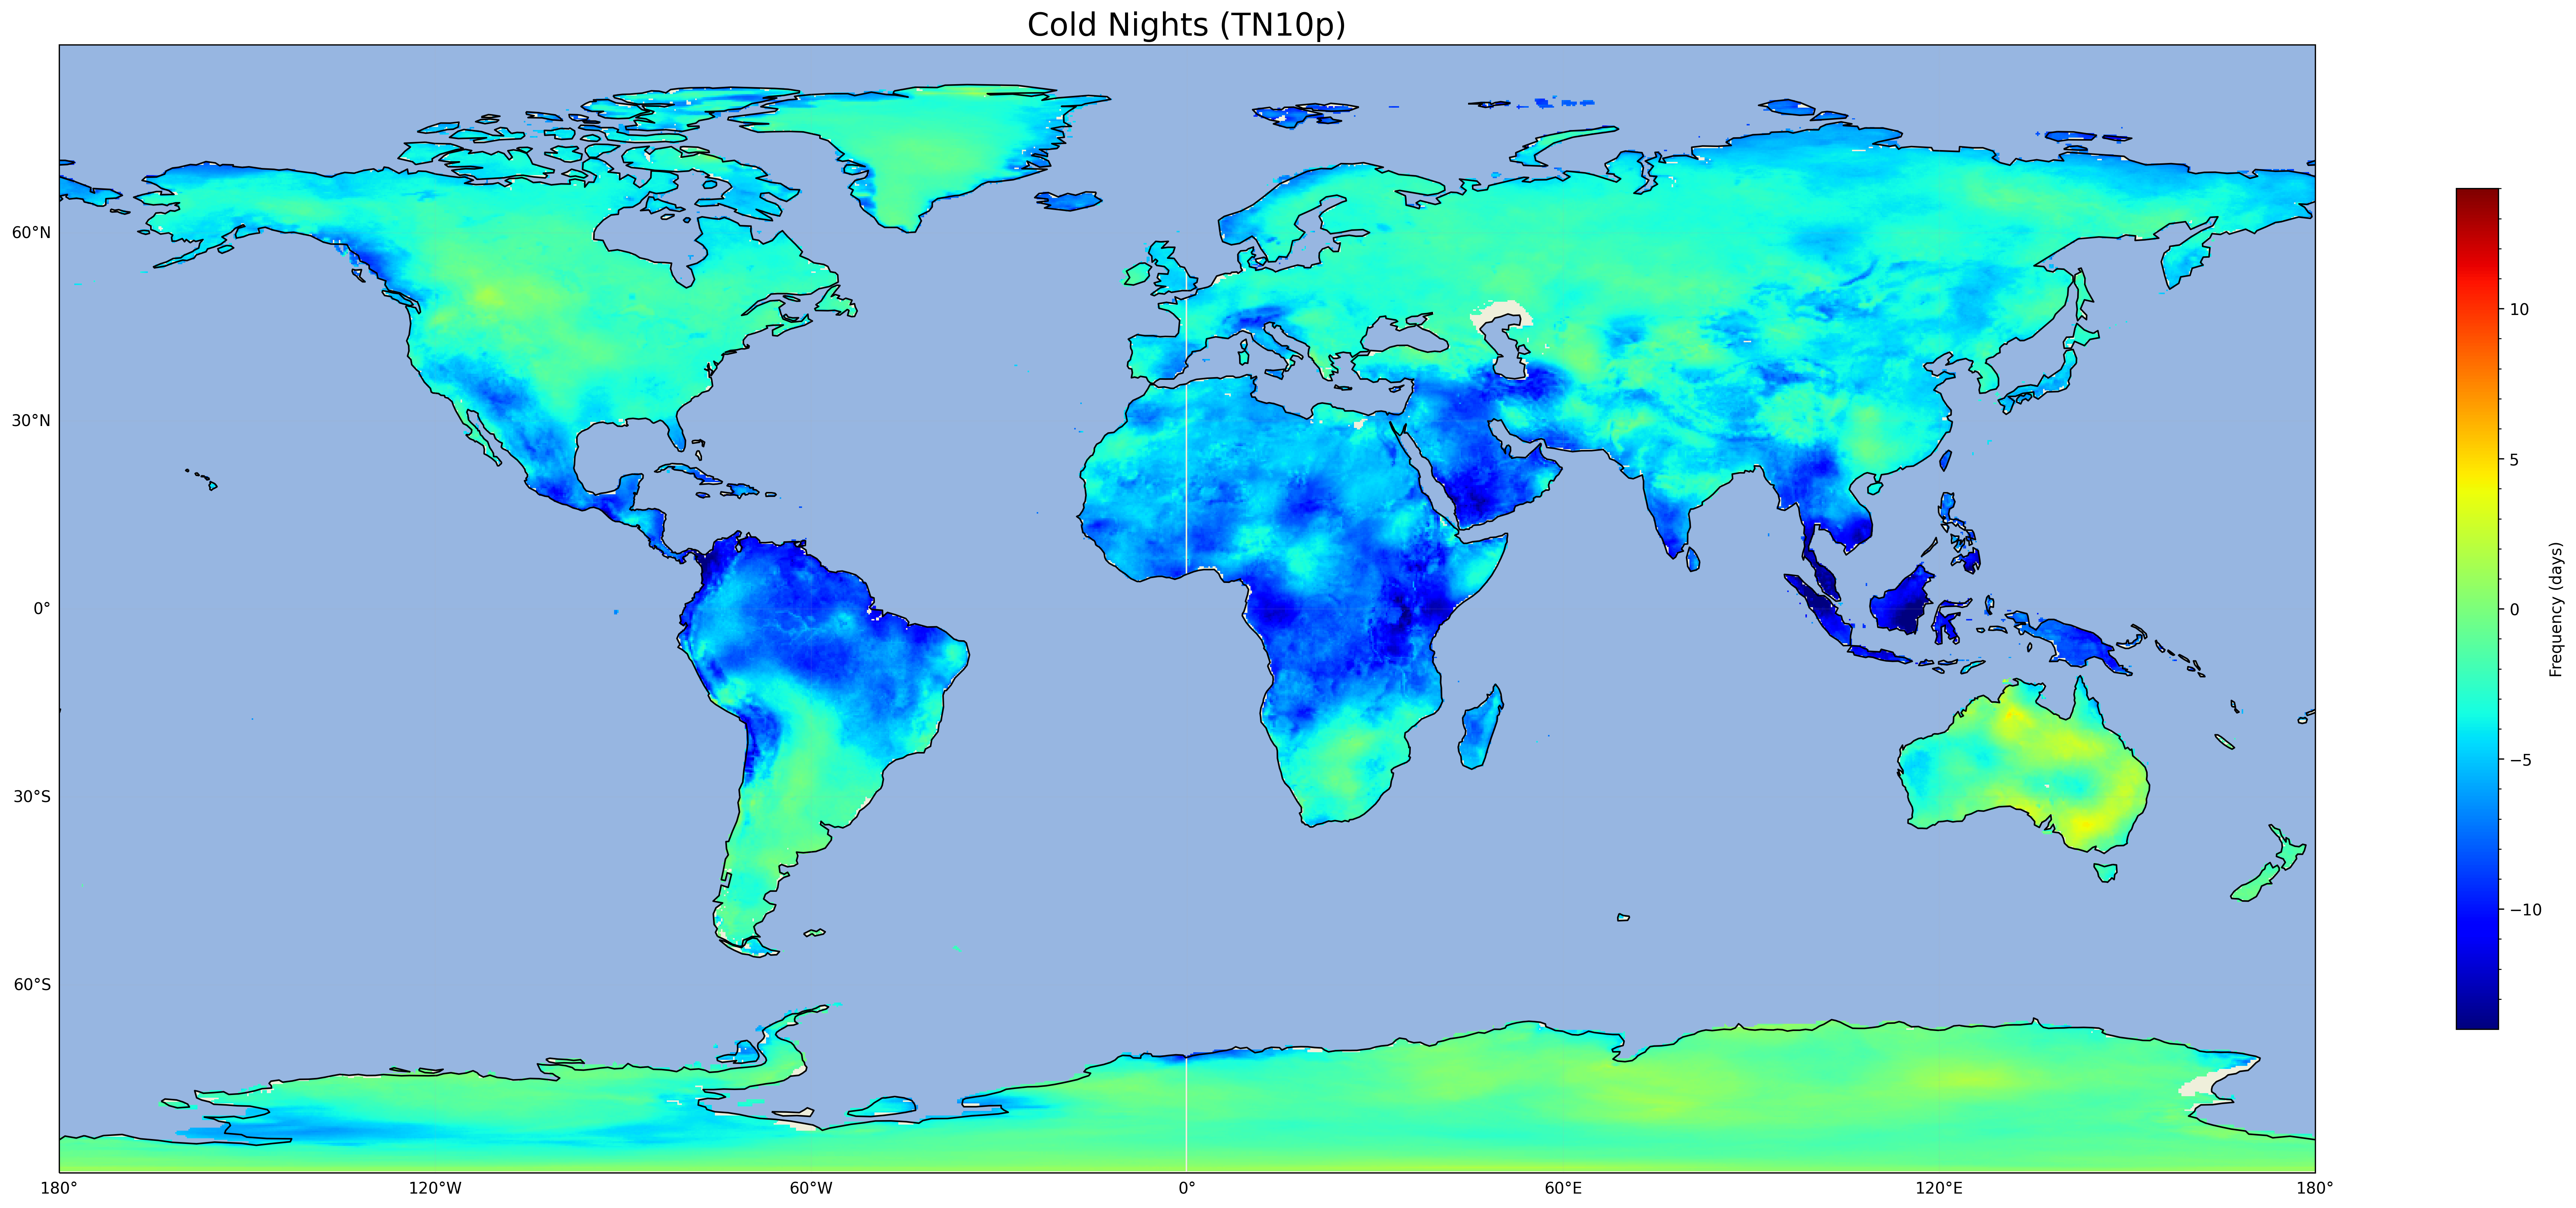
\includegraphics[width=0.80\textwidth]{/home/shiv/Documents/GitHub/EES405/clim_extreme/plots_clim_extreme/cold_nights.png}
%     \caption{Warm days Spatial Plot}
%     \label{fig:rx5_jja_spatial}
% \end{figure}

\subsection{Temporal Plot for '5-day precipitation amount (RX5) for JJA season'}
In the above time series plot of 5-day precipitation amount anomalies for (JJA) months calculated from the \textbf{RX5} climate index, we have added a non-linear trendline with polynomial fit of degree 21 (as used in the paper by )given by the following equation.
\begin{figure}[htb]
    \centering
    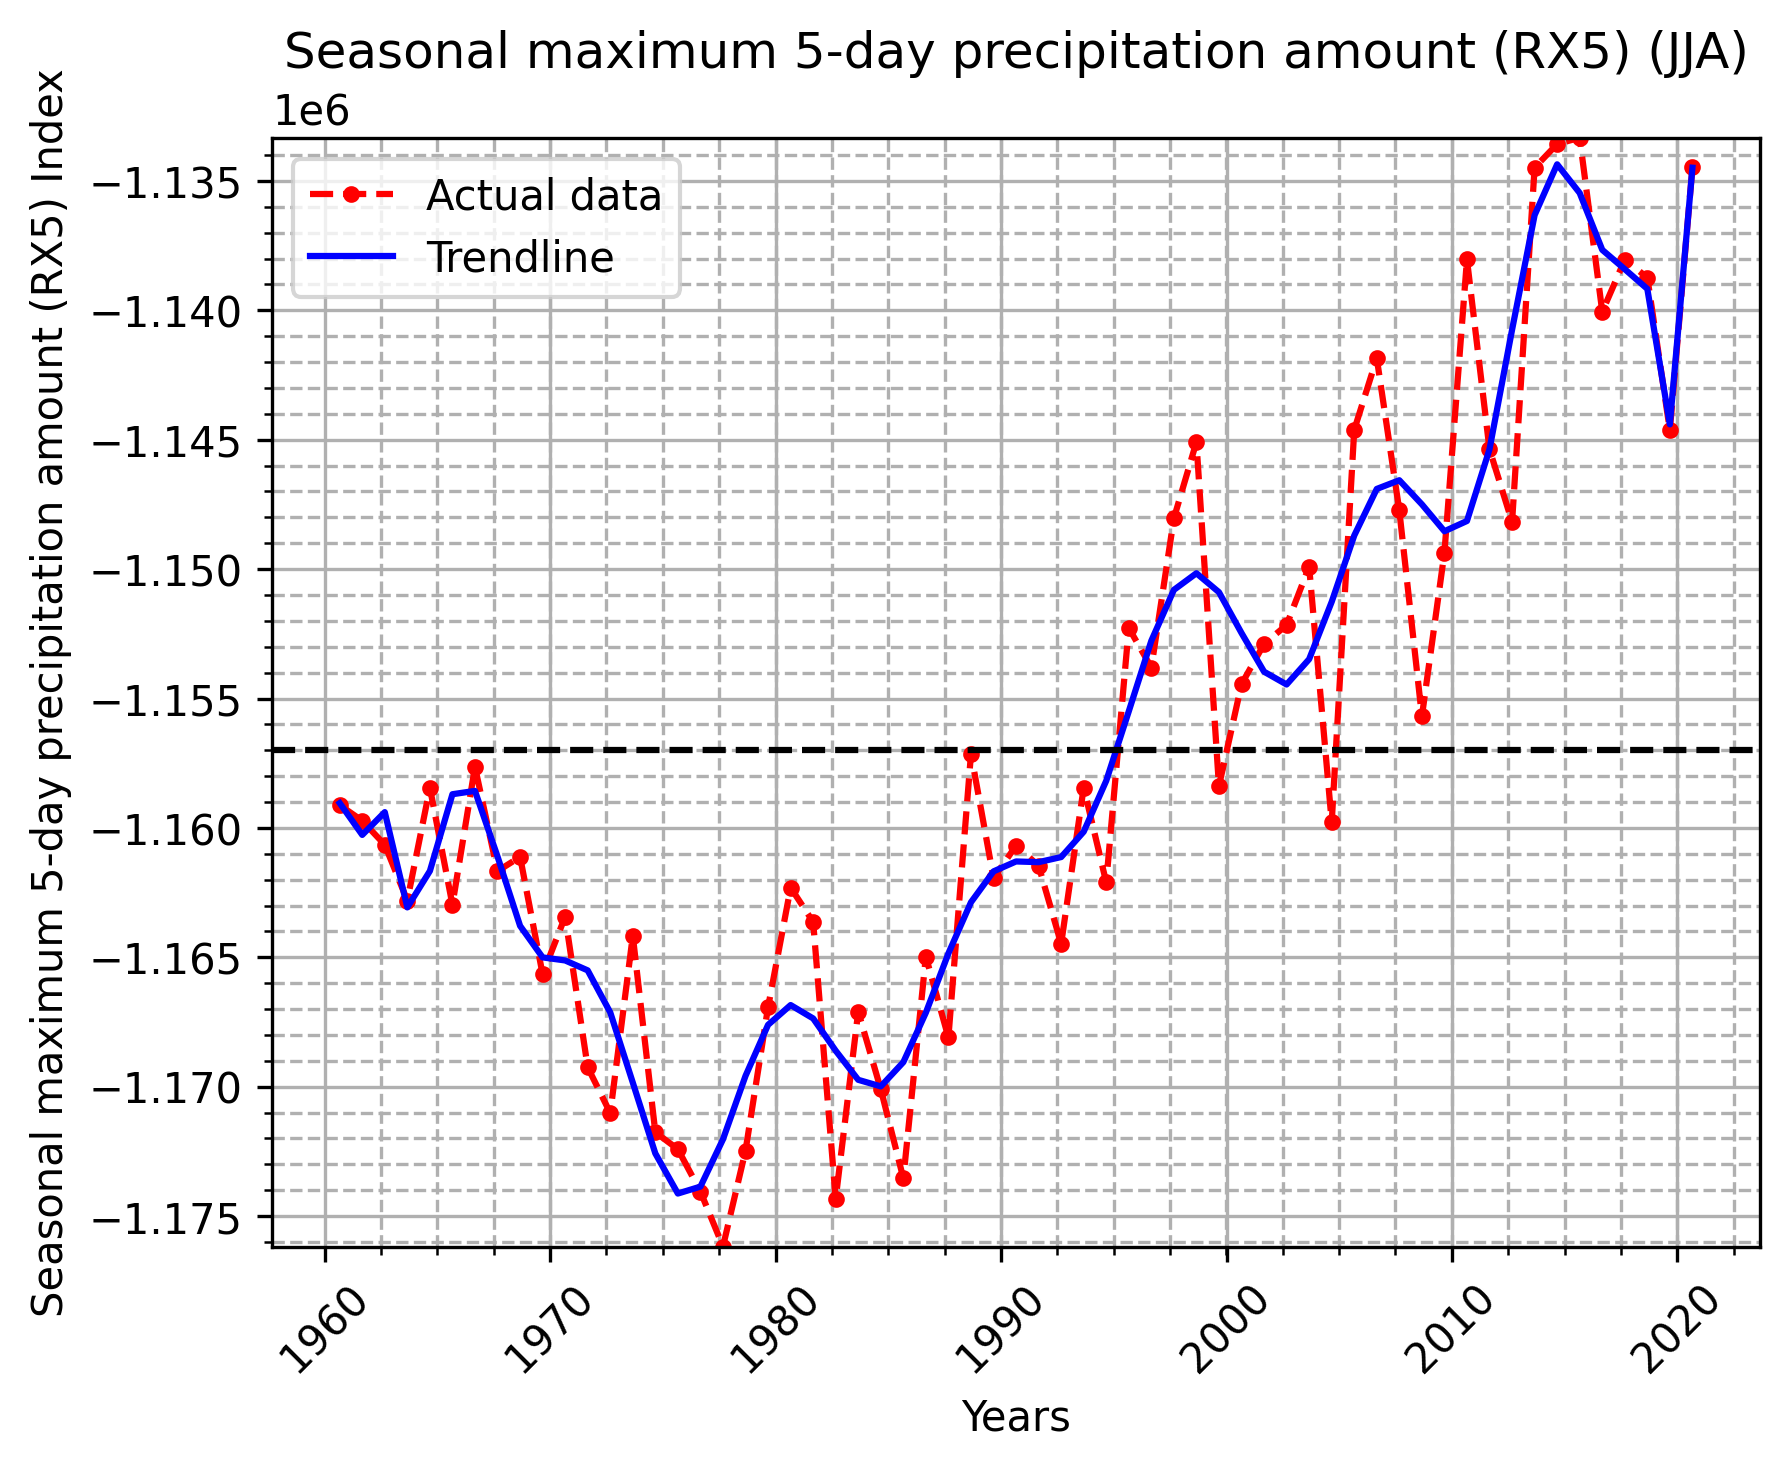
\includegraphics[width=0.75\textwidth]{//home/shiv/Documents/GitHub/EES405/clim_indices/final_plots/rx5_jja.png}
    \caption{5-day precipitation amount (RX5) (JJA) temporal Plot}
    \label{fig:rx5_jja_temporal}
\end{figure}

$ y = -3.42\times10^{3}x^{21}+7.44\times10^{-5}x^{20}-1.88\times10^{-6}x^{19}+3.31\times10^{-10}x^{18}+1.08\times10^{-12}x^{17}-3.97\times10^{-16}x^{16}-1.62\times10^{-19}x^{15}+1.05\times10^{-22}x^{14}-5.80\times10^{-27}x^{13}-8.00\times10^{-30}x^{12}+2.29\times10^{-33}x^{11}-1.20\times10^{-37}x^{10}-6.72\times10^{-41}x^{9}+1.99\times10^{-44}x^{8}-2.95\times10^{-48}x^{7}+2.85\times10^{-52}x^{6}-1.92\times10^{-56}x^{5}+9.12\times10^{-61}x^{4}-3.03\times10^{-65}x^{3}+6.69\times10^{-70}x^{2}-8.87\times10^{-75}x+5.34\times10^{-80}$

The incease in the frequency of 5-day precipitation amount is consistent with the overall warming of the planet due to climate change as seen in the above spatial plot.\\
Overall, the increase in the frequency of 5-day precipitation amount is a consistent and expected result of the overall warming of the planet due to climate change.


% \subsection{Spatial plot for 5-day precipitation amount (RX5) for SON season}
% \begin{figure}[htb]
%     \centering
%     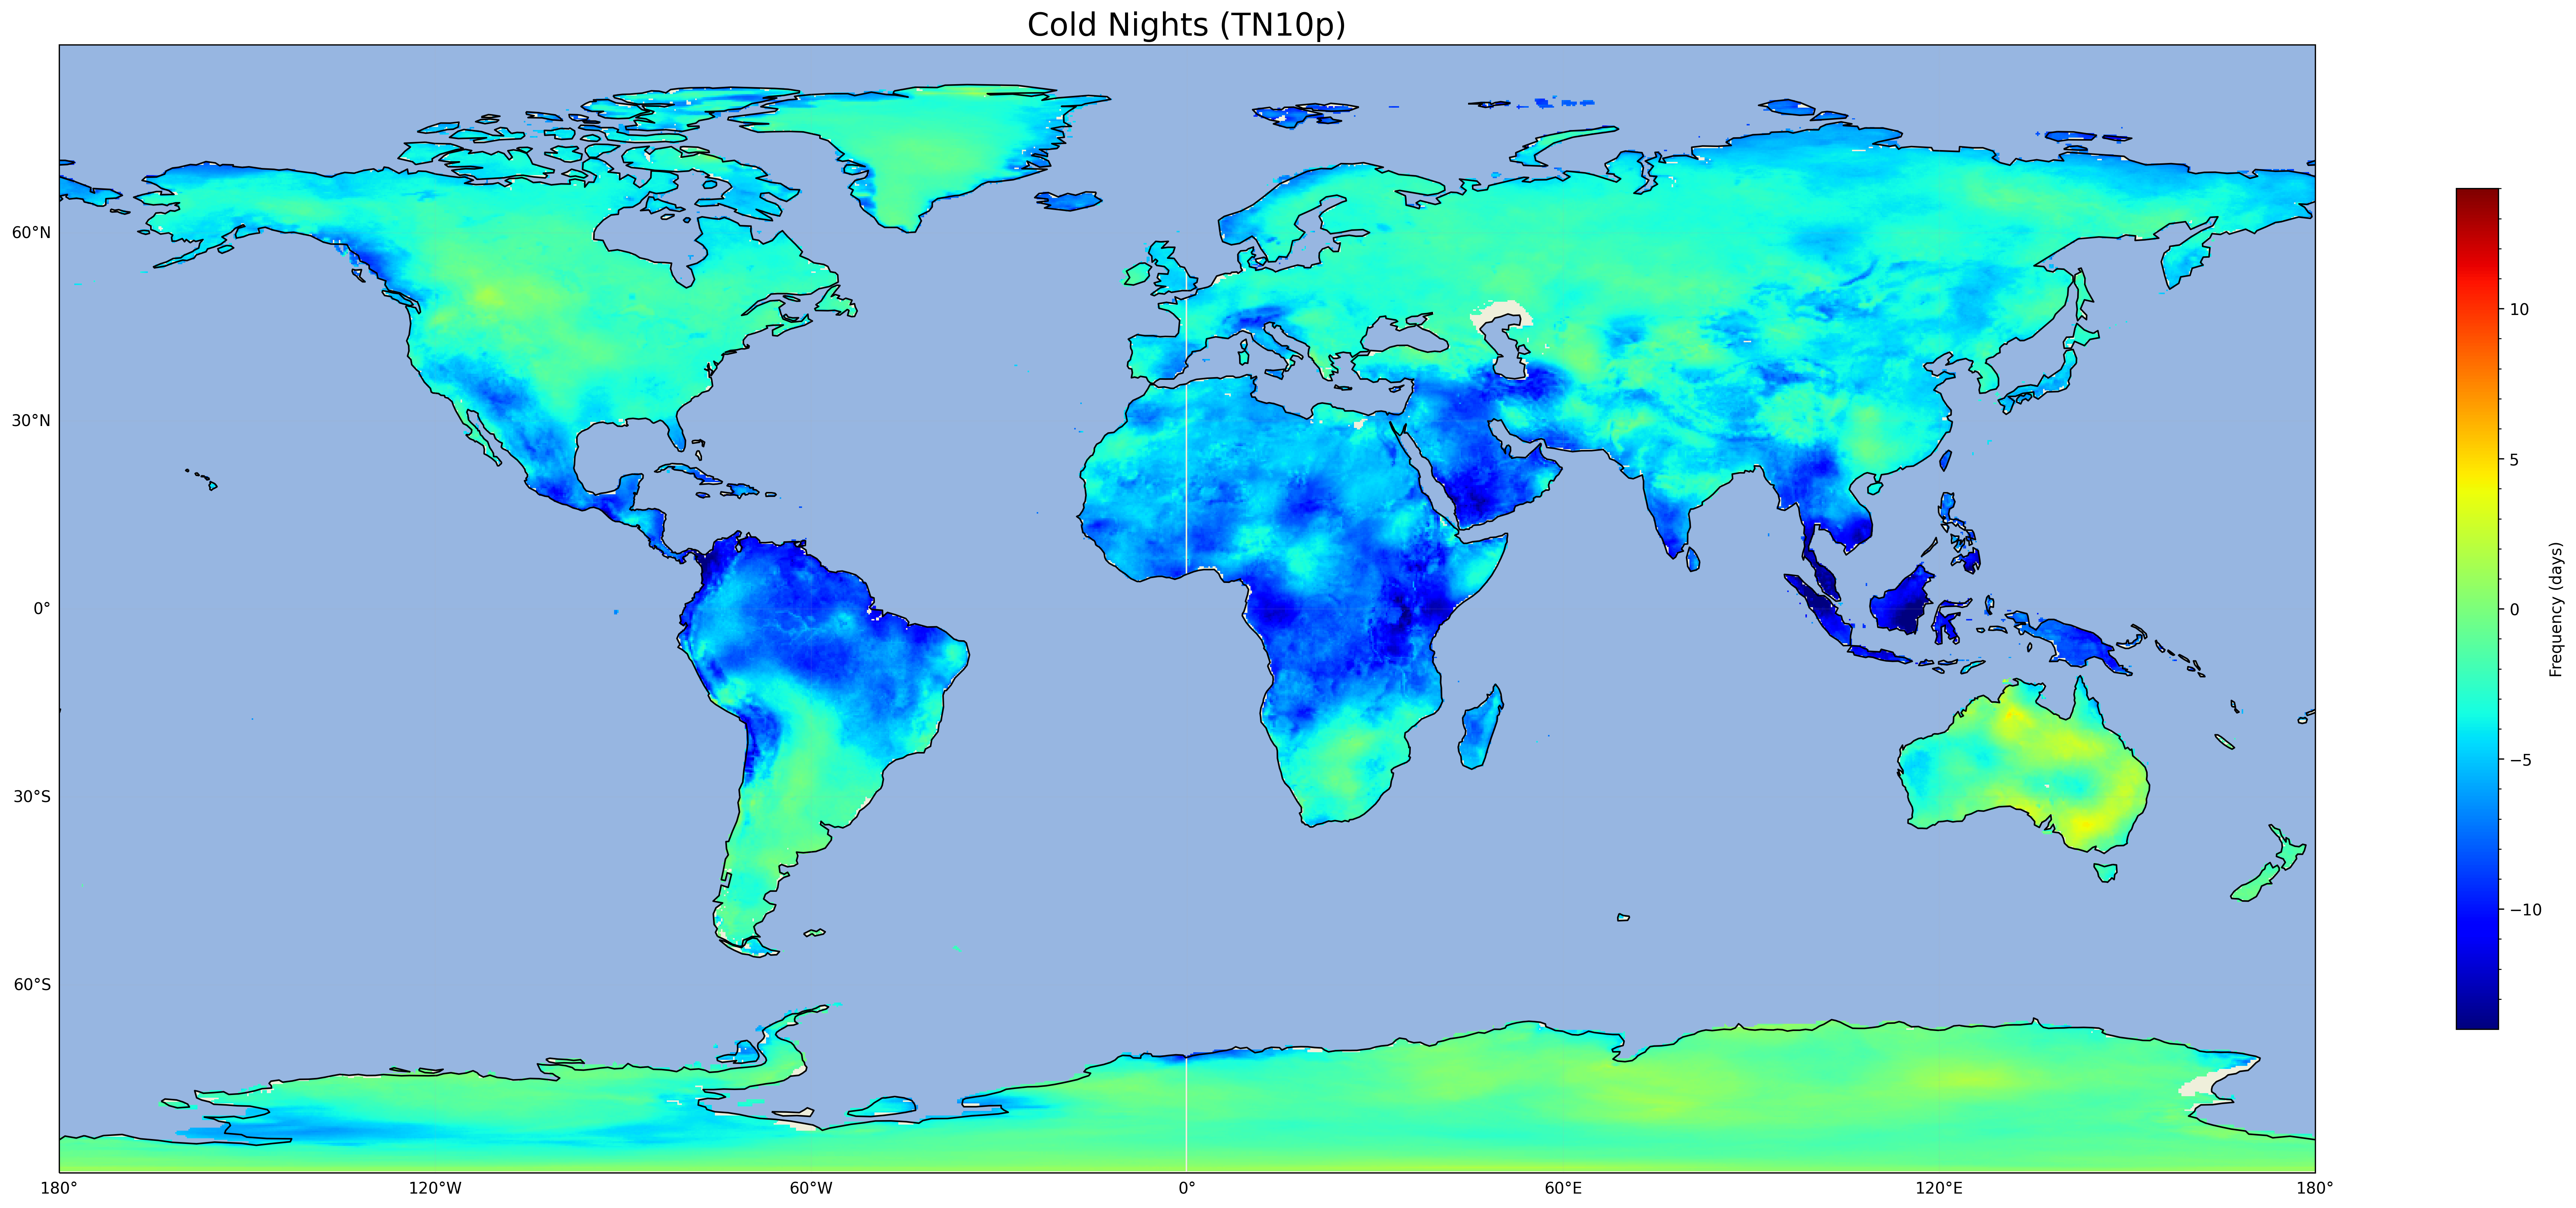
\includegraphics[width=0.80\textwidth]{/home/shiv/Documents/GitHub/EES405/clim_extreme/plots_clim_extreme/cold_nights.png}
%     \caption{Warm days Spatial Plot}
%     \label{fig:rx5_son_spatial}
% \end{figure}

\subsection{Temporal Plot for '5-day precipitation amount (RX5) for SON season'}
In the above time series plot of 5-day precipitation amount anomalies for (SON) months calculated from the \textbf{RX5} climate index, we have added a non-linear trendline with polynomial fit of degree 21 (as used in the paper by )given by the following equation.
\begin{figure}[htb]
    \centering
    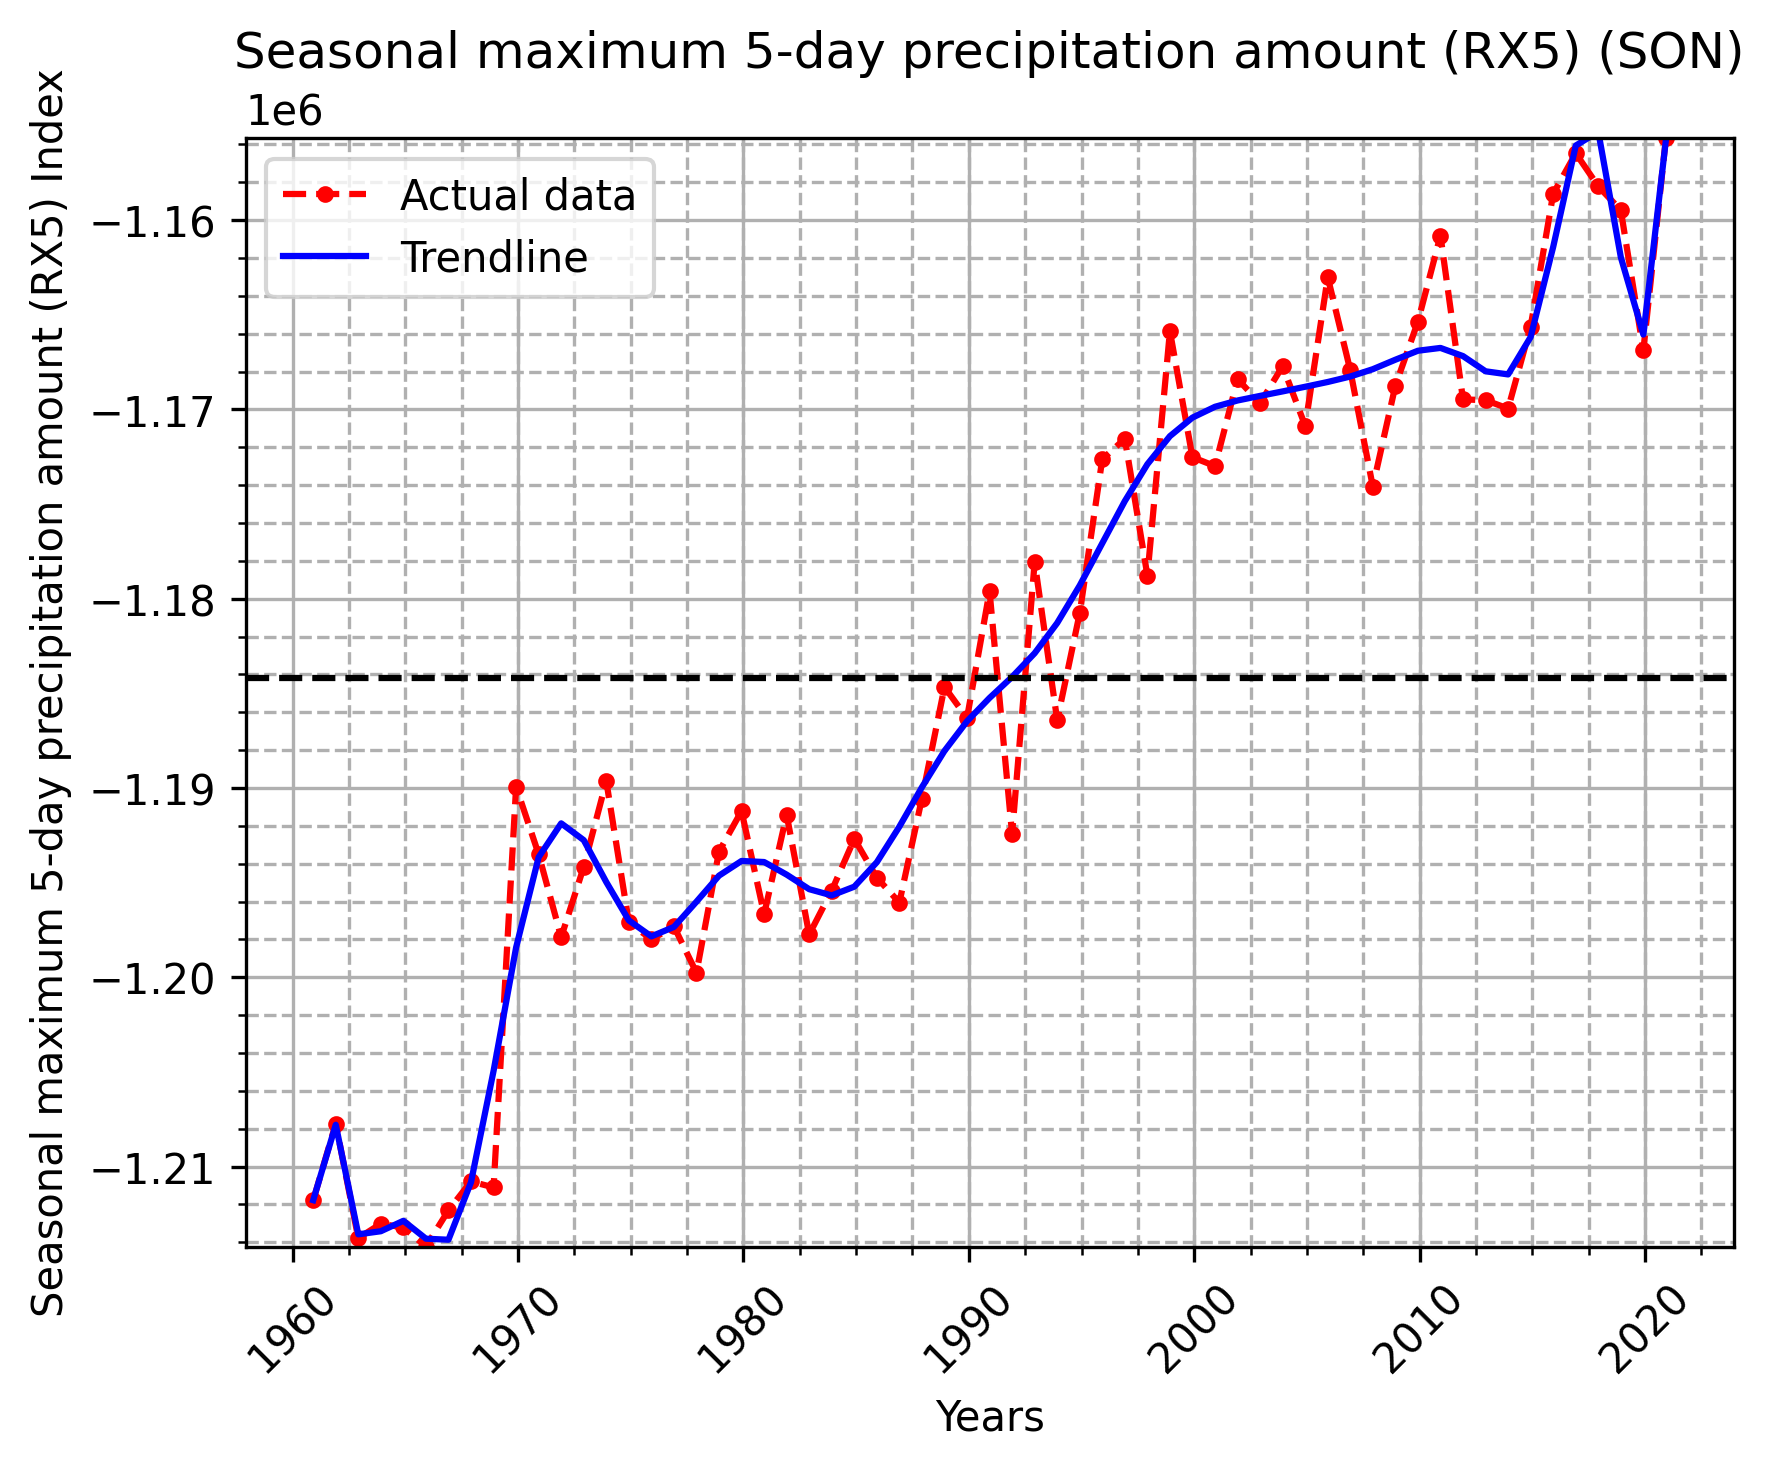
\includegraphics[width=0.75\textwidth]{//home/shiv/Documents/GitHub/EES405/clim_indices/final_plots/rx5_son.png}
    \caption{5-day precipitation amount (RX5) (SON) temporal Plot}
    \label{fig:rx5_son_temporal}
\end{figure}

$ y = -3.42\times10^{3}x^{21}+7.44\times10^{-5}x^{20}-1.88\times10^{-6}x^{19}+3.31\times10^{-10}x^{18}+1.08\times10^{-12}x^{17}-3.97\times10^{-16}x^{16}-1.62\times10^{-19}x^{15}+1.05\times10^{-22}x^{14}-5.80\times10^{-27}x^{13}-8.00\times10^{-30}x^{12}+2.29\times10^{-33}x^{11}-1.20\times10^{-37}x^{10}-6.72\times10^{-41}x^{9}+1.99\times10^{-44}x^{8}-2.95\times10^{-48}x^{7}+2.85\times10^{-52}x^{6}-1.92\times10^{-56}x^{5}+9.12\times10^{-61}x^{4}-3.03\times10^{-65}x^{3}+6.69\times10^{-70}x^{2}-8.87\times10^{-75}x+5.34\times10^{-80}$

The incease in the frequency of 5-day precipitation amount is consistent with the overall warming of the planet due to climate change as seen in the above spatial plot.\\
Overall, the increase in the frequency of 5-day precipitation amount is a consistent and expected result of the overall warming of the planet due to climate change.



\end{document}








